% load lecture note class
\documentclass{easyclass}
\usepackage{float} 
\begin{document}
\begin{titlepage}
    \university{UNIVERSIDAD ADOLFO IBÁÑEZ}
    \courseid{ECO -TS101}
    \title{Lecture Note: Econometr\'\i{}a de Series de Tiempo }
    \author{Marcelo Villena Chamorro PhD.}
    \version{2019 Winter}
    \instructor{Instructor: ~ \textsc{Marcelo Villena Chamorro PhD.}\par}
    \maketitle
\end{titlepage}

\tableofcontents

\chapter{Tópico I.- Introducción a la Econometría de Series de Tiempo}

\section{La naturaleza de los datos de serie de tiempo}

El objetivo principal del an\'alisis de series temporales es desarrollar modelos matem\'aticos que proporcionen descripciones plausibles para los datos de la muestra.
\\
Existen dos enfoques metodol\'ogicos b\'asicos para modelar series de tiempo:

	\begin{itemize}
		\item[(i)] El enfoque del dominio del tiempo (Time domain approach)
		\item[(ii)] El enfoque de dominio de frecuencia (Frequency domain approach)
	\end{itemize}

\begin{frame}

El \textbf{enfoque del dominio del tiempo} generalmente est\'a motivado por la presunci\'on de que la correlaci\'on entre los puntos adyacentes en el tiempo de los datos de una serie, se explica mejor en t\'erminos de una dependencia del valor actual en valores pasados. De esta forma, \'este enfoque se centra en modelar alg\'un valor futuro de una serie temporal como una función param\'etrica de los valores actuales y pasados.
\\
En este escenario, por ejemplo, utilizamos modelos de regresiones lineales sobre el valor actual de una serie temporal, utilizando como variables de lado derecho a sus propios valores pasados y los valores pasados de otras series. El seminal trabajo de Box y Jenkins y sus modelos autoregresivos (ARIMA), se encuentran en esta l\'\i{}nea, ver \cite{BoxJenkins}.

\end{frame}

\begin{frame}

Por otro lado, \textbf{el enfoque de dominio de frecuencia} asume que las caracter\'\i{}sticas principales de inter\'es en el an\'alisis de las series de tiempo se relacionan con variaciones sinusoidales peri\'odicas o sistem\'aticas que se encuentran naturalmente en la mayor\'\i{}a de los datos.
\\
Estas variaciones peri\'odicas a menudo son causadas por fen\'omenos biol\'ogicos, f\'\i{}sicos o ambientales de inter\'es. El estudio de la periodicidad se extiende a la econom\'\i{}a y las ciencias sociales, donde uno puede estar interesado en las periodicidades anuales en series como el desempleo mensual o las tasas mensuales de natalidad.
\\
En el an\'alisis espectral, la partici\'on de los diversos tipos de variaci\'on peri\'odica en una serie temporal se lleva a cabo evaluando separadamente la varianza asociada con cada tipo de periodicidad.

\end{frame}
\pagebreak
%\begin{frame}
\subsection{Ejemplo 1: Cambio climático}Nuestro primer ejemplo de serie de tiempo es la temperatura de la tierra. Observamos una aparente tendencia ascendente en la serie durante la \'ultima parte del siglo XX, la que se ha utilizado como argumento para la hip\'otesis del calentamiento global. N\'otese tambi\'en la tendencia ascendente y bastante pronunciada alrededor de 1970. La cuesti\'on de inter\'es para los defensores del calentamiento global y los oponentes es si la tendencia general es natural, o si por el contrario es causada por el ser humano.

\begin{figure}[H]{}
	\centering
	\textbf{Ejemplo 1: Cambio climático}\par\medskip
	\fcolorbox{green}{blue}{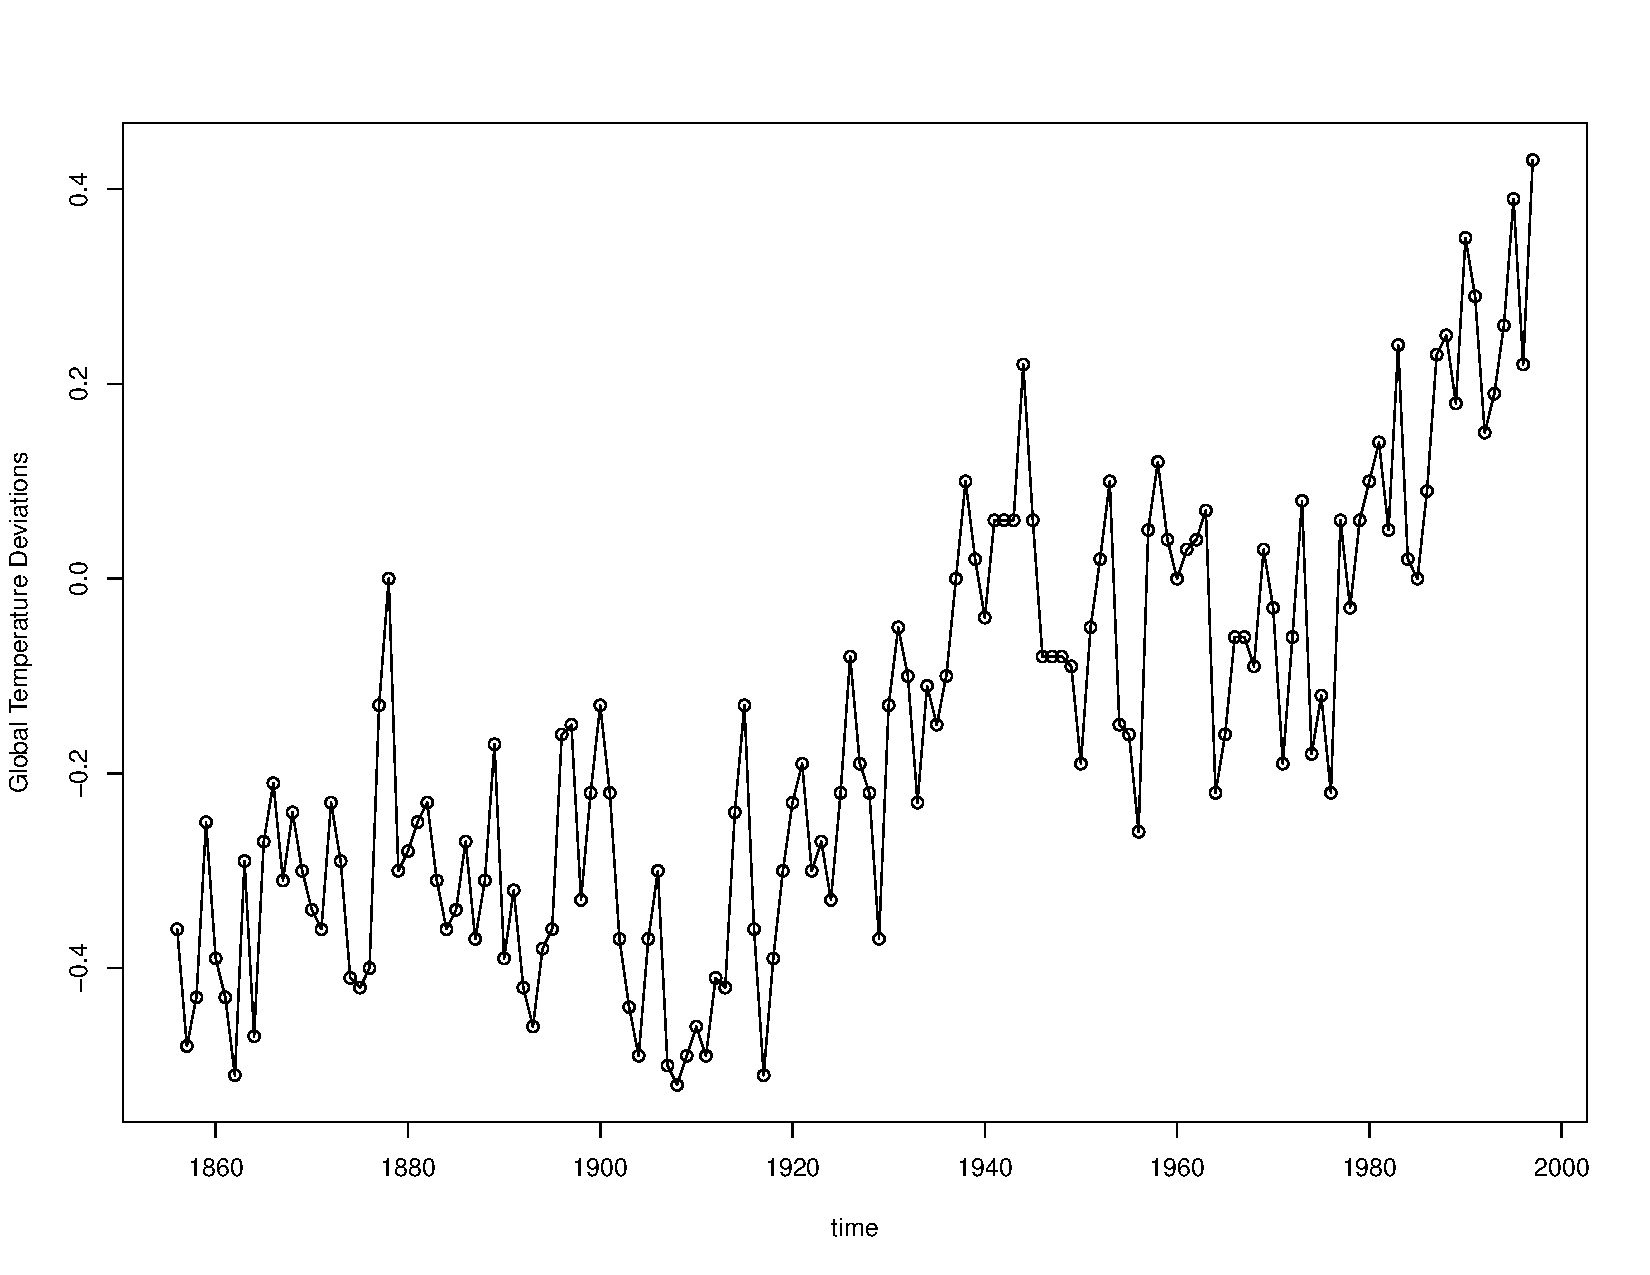
\includegraphics[width=\linewidth]{gtemp.pdf}}
	\caption{Cambio clim\'atico: mediciones de temperatura desde 1860}\label{figura1}
\end{figure}
%\end{frame}

%\centering
\lstset{caption=Código R para ejemplo del cambio climático,framexleftmargin=5mm, frame=shadowbox, rulesepcolor=\color{green}}
\pagebreak
\begin{lstlisting}[title={‘Código R  para ejemplo del cambio climático.’},basicstyle=\ttfamily]{}
# Set the working directory
setwd("/Users/Desktop/Econometrics/Clase 1.- TSE")
# Limpiar_variables
rm(list=ls())

install.packages("tidyverse")
install.packages("dplyr")
install.packages("tseries")

mydata<-read.csv ("gtemp.csv")
plot(mydata, type="o", ylab="Global Temperature Deviations")
\end{lstlisting}

%---------------------Slide 9 --------------------------
%\begin{frame}
\subsection{Ejemplo 2: Series temporales financieras}
%\frametitle{Ejemplo 2: Series temporales financieras}
En finanzas siempre es preferible trabajar con el retorno (returns) de los activos, en vez de usar directamente el precio de los activos. Existen dos maneras de convertir el precio en retornos:
\begin{equation*}
R_t = \frac{p_t - p_{t-1}}{p_{t-1}} *100%
\end{equation*}
\\
\begin{equation*}
R_t = ln\left(\frac{p_t}{p_{t-1}}\right)*100%
\end{equation*}
where, $R_t$ denota el retorno al tiempo $t$, $p_t$ denota el precio del activo al tiempo $t$, y $ln$ denota el logaritmo natural. En esta formulaci\'on ignoramos los dividendos, o asumimos que las series de precios ya han sido ajustadas por ellos.

%\end{frame}
%---------------------Slide 10 --------------------------
%\begin{frame}
%\frametitle{Ejemplo 2: Series temporales financieras}
Los log-returns tienen la deseable propiedad de poder ser interpretados como rendimientos continuamente compuestos. Adem\'as, ellos pueden ser simplemente sumados, de forma de obtener retornos con respecto a per\'\i{}odos m\'as largos:
\begin{center}
	$r_1 = ln \frac{p_1}{p_0} = ln p_1 - ln p_0$\\
	$r_2 = ln \frac{p2}{p_1} = ln p_2 - ln p_1$\\
	$r_3 = ln \frac{p3}{p_2} = ln p_3 - ln p_2$\\
	$r_4 = ln \frac{p4}{p_3} = ln p_4 - ln p_3$\\
	$r_5 = ln \frac{p5}{p_4} = ln p_5 - ln p_4$\\	
	\vspace{5mm}	     			      
	$r_1+r_2+r_3+r_4+r_5=ln p_5 - ln p_0    =  ln \frac{p_5}{p_0}$\\
\end{center}
%\end{frame}
%---------------------------------------------------------
%\begin{frame}
%\frametitle{Ejemplo 2: Series temporales financieras}
\subsubsection{Ejemplo 2: Series temporales financieras}
Como segundo ejemplo calcularemos los retornos de la Bolsa de Nueva York, \'\i{}ndice "S$\&$P 500", extrayendo data diaria desde el a\~no 2000, del sitio: https://finance.yahoo.com/\\

%\only<1|handout:1>{
	%\begin{exampleblock}{C\'odigo en R}
\lstset{caption=Código R precio de la Bolsa de Nueva York,framexleftmargin=5mm, frame=shadowbox, rulesepcolor=\color{green}}
\begin{lstlisting}[title={‘Código R precio de la Bolsa de Nueva York.’},basicstyle=\ttfamily]{}
mydata2<-read.csv("sp.csv")
precio<-mydata2$"Adj.Close"
plot.ts(precio, type="o", ylab="Precio Bolsa de Nueva York")
lnprecio <- log10(precio)
Dlnprecio <- diff(lnprecio,1)
plot.ts(Dlnprecio, type="o", ylab="Retorno Bolsa de Nueva York")
summary (lnprecio)
summary (Dlnprecio)
\end{lstlisting}

%\end{exampleblock}
%}
%\end{frame}
%---------------------------------------------------------
%---------------------Slide 12 --------------------------
%\begin{frame}
%\frametitle{Ejemplo 2: Series temporales financieras}
%\textbf{Indice Bolsa de Nueva York}
%\end{frame}
\begin{figure}[H]{}
\centering
\textbf{Ejemplo 2: Series temporales financieras}\par\medskip
\fcolorbox{green}{blue}{
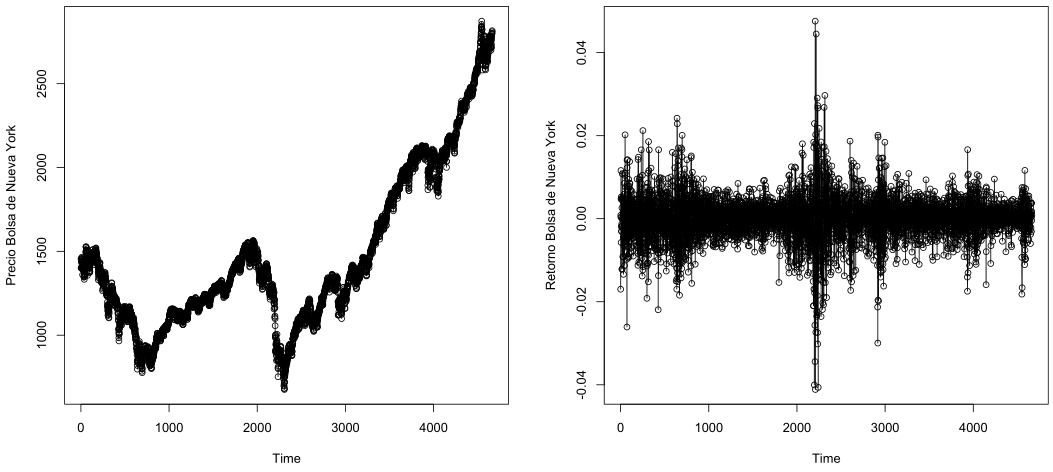
\includegraphics[width=\linewidth]{bolsaNYD12.png}}
\caption{Indice Bolsa de Nueva York. Izquierda: precios reales SP500. Derecha: retornos SP500.}\label{figura2}
\end{figure}

%---------------------------------------------------------
%---------------------Slide 13 --------------------------
%\begin{frame}
%\frametitle{Ejemplo 2: Series temporales financieras}
Los precios al parecer no son normales, aparentemente son log-normales.\\
\begin{figure}[H]
	\centering
	\textbf{Ejemplo 2: Histograma de los Precios}\par\medskip
	\fcolorbox{green}{blue}{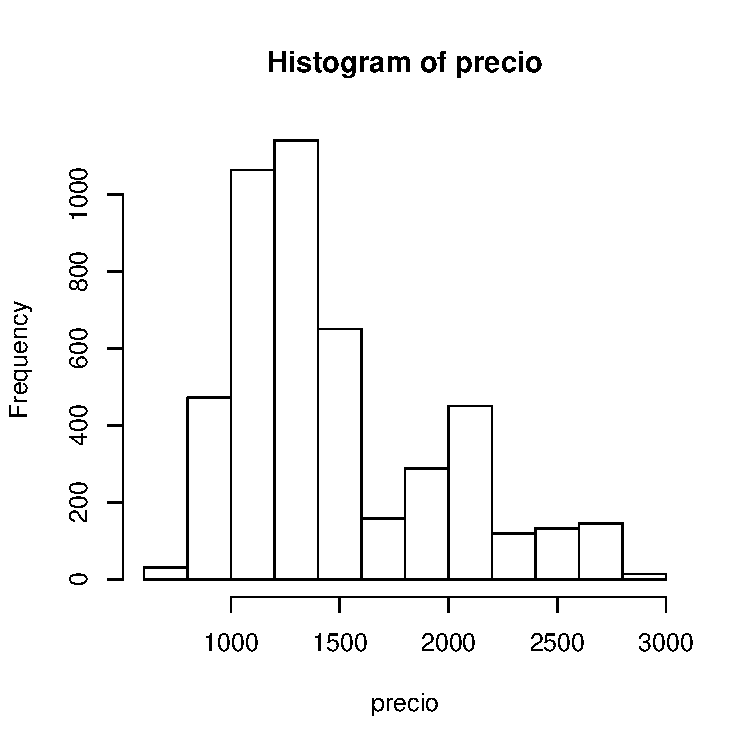
\includegraphics[width=\linewidth]{hist_precio_sp.pdf}}
	\caption{Histograma de los precios de la Bolsa de NY}\label{figura3}
\end{figure}
%\end{frame}

%---------------------------------------------------------
%---------------------Slide 14 --------------------------
%\begin{frame}
%\frametitle{Ejemplo 2: Series temporales financieras}
\pagebreak
Los retornos de los precios si parecen normales~\ref{figura4}, lo cual constituye una propiedad deseable para el an\'alisis estad\'\i{}stico.\\
\begin{figure}[H]
	\centering
	\textbf{Ejemplo 2: Histograma de los Precios}\par\medskip
	\fcolorbox{green}{blue}{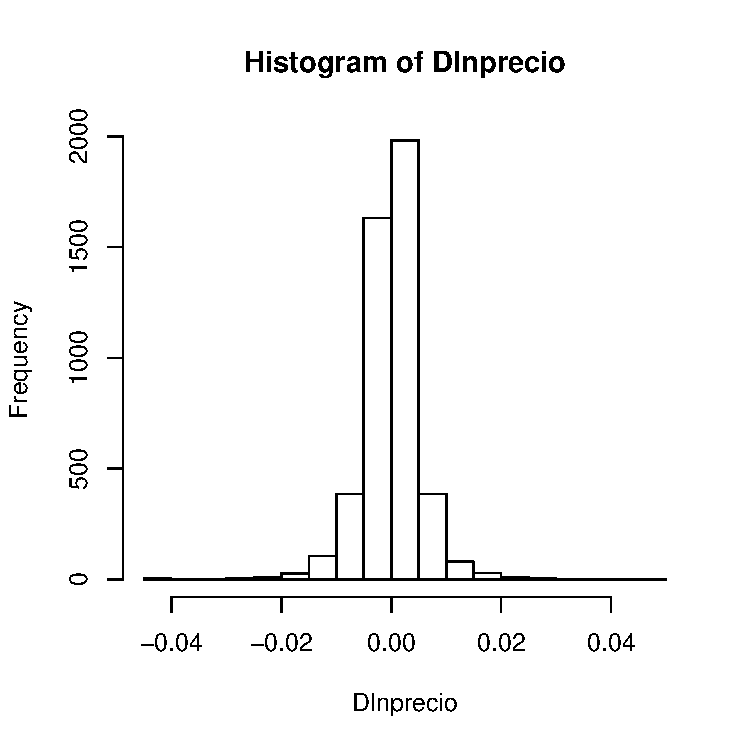
\includegraphics[width=\linewidth]{hist_dlnprecio_sp.pdf}}
	\caption{Histograma de los retornos de la Bolsa de NY}\label{figura4}
\end{figure}
%\end{frame}

%\end{section}
%---------------------------------------------------------
%---------------------Slide 15 --------------------------
%\begin{frame}
%\frametitle{Ejemplo 2: Series temporales financieras}
\begin{figure}[H]
	\centering
	\textbf{Ejemplo 2: Histograma de los Precios}\par\medskip
	\fcolorbox{green}{blue}{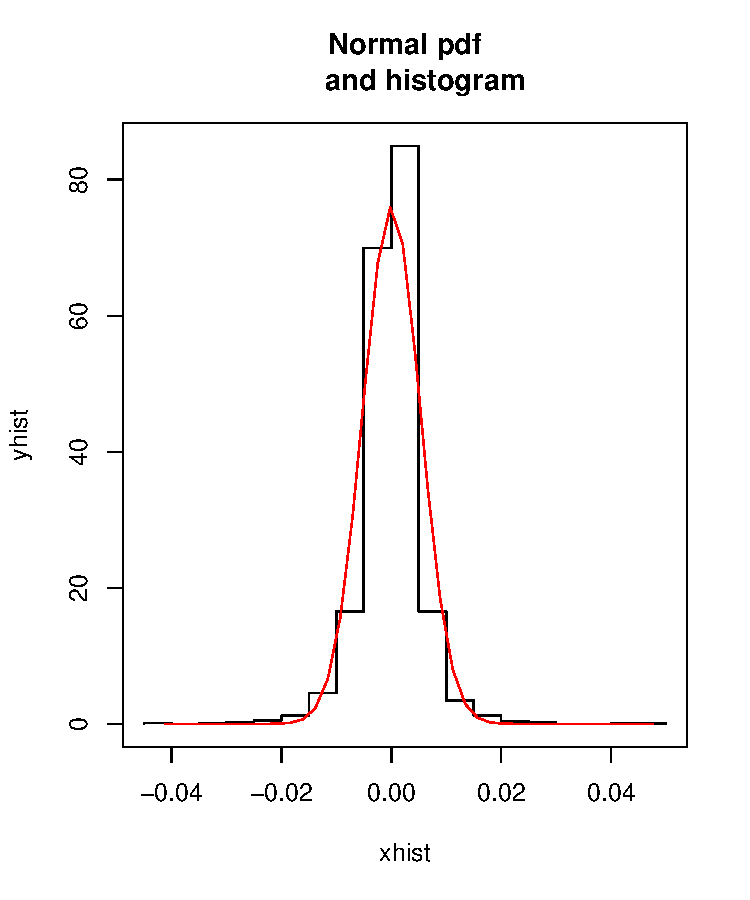
\includegraphics[width=\linewidth]{normal_hist_Dlnprice_sp.pdf}}
	\caption{Linea negra:Histograma de las diferencias de los log-precios de la Bolsa de NY. Linea roja: ajuste de la distribución normal segúun media y desviación estandar de la muestra. Shapiro-Wilk normality test / data:  Dlnprecio / W = 0.90927, p-value $<$ 2.2e-16.}\label{figura5}
\end{figure}
%Shapiro-Wilk normality test
%data:  Dlnprecio
%W = 0.90927, p-value $<$ 2.2e-16.
%\end{frame}

%---------------------------------------------------------
%---------------------Slide 16 --------------------------
%\begin{frame}
%\frametitle{Ejemplo 2: Series temporales financieras}
%
%\only<1|handout:1>{
	%\begin{exampleblock}{C\'odigo en R}
%		h $<-$ hist(Dlnprecio,breaks=15)\\
%		xhist $<-$ c(min(h\$breaks),h\$breaks)\\
%		yhist $<-$ c(0,h\$density,0)\\
%		xfit $<-$ seq(min(Dlnprecio),max(Dlnprecio),length=40)\\
%		yfit $<-$ dnorm(xfit,mean=mean(Dlnprecio),sd=sd(Dlnprecio))\\
%		plot(xhist,yhist,type="s",ylim=c(0,max(yhist,yfit)), main=``Normal pdf and histogram")\\
%		lines(xfit,yfit, col=``red")\\
%		shapiro.test(Dlnprecio)
	%\end{exampleblock}
%}
%\end{frame}
\pagebreak
\lstset{caption = Código R de histograma y ajuste de curva normal,framexleftmargin=5mm, frame=shadowbox, rulesepcolor=\color{green}}
\begin{lstlisting}[title={‘Código R de histograma y ajuste de curva normal’},basicstyle=\ttfamily]{}
h <- hist(Dlnprecio,breaks=15)
xhist <- c(min(h$breaks),h$breaks)
yhist <- c(0,h$density,0)
xfit <- seq(min(Dlnprecio),max(Dlnprecio),length=40)
yfit <- dnorm(xfit,mean=mean(Dlnprecio),sd=sd(Dlnprecio))
plot(xhist,yhist,type="s",ylim=c(0,max(yhist,yfit)), 
	main="Normal pdf and histogram")
lines(xfit,yfit, col="red")
shapiro.test(Dlnprecio)
\end{lstlisting}

%---------------------------------------------------------
%---------------------Slide 17 --------------------------
%\begin{section}{Modelamiento estad\'istico de las series de tiempo}
\section{Modelamiento estad\'istico de las series de tiempo}
%	\begin{frame}
%	\frametitle{Modelos estad\'isticos de series de tiempo}
	Para poder modelar los datos, que aparentemente fluct\'uan de forma aleatoria a lo largo del tiempo, suponemos que una serie temporal se define como una colecci\'on de variables aleatorias. 
	\\
	Por ejemplo, podemos modelar  una serie temporal como una secuencia de variables aleatorias, $x_1, x_2, x_3,...$, donde la variable aleatoria $x_1$ denota el valor tomado por la serie en el primer punto de tiempo, la variable $x_2$  denota el valor para el segundo per\'\i{}odo de tiempo, y as\'\i{} sucesivamente. 
	\\
	En general, una colecci\'on de variables aleatorias,  $\{x_t\}$, indexada por t se conoce como proceso estoc\'astico. En este texto, $t$ ser\'a t\'\i{}picamente discreto y variar\'a sobre los enteros $t = 0, \pm1, \pm2,,.... $, o alg\'un subconjunto de los enteros. Los valores observados en un proceso estoc\'astico se conocen como la realizaci\'on del proceso estoc\'astico.	
%\end{frame}
%---------------------------------------------------------
%---------------------Slide 18 --------------------------
%\begin{frame}
%\frametitle{Ruido blanco - White Noise}
\subsection{Ruido blanco - White Noise}
Una serie de tiempo muy utilizada es aquella representada por una colecci\'on de variables aleatorias no correlacionadas, $\epsilon_t$, con media $0$ y varianza finita $\sigma^2_\epsilon$. Las series temporales generadas a partir de variables no correlacionadas se utilizan por ejemplo para modelar el ruido en aplicaciones de ingenier\'\i{}a, donde se denomina ruido blanco. A veces denotaremos este proceso como $\epsilon_t$$\sim$$\epsilon_n (0, \sigma^2_\epsilon)$. La designaci\'on de "blanco" se origina de la analog\'\i{}a con la luz blanca e indica que todas las posibles oscilaciones peri\'odicas est\'an presentes con la misma fuerza.

%\end{frame}
%---------------------------------------------------------
%---------------------Slide 19 --------------------------
%\begin{frame}
%\frametitle{Ruido blanco - White Noise}

\begin{itemize}
	\item En ocasiones, tambi\'en requeriremos que el ruido sea independiente y tenga una distribuci\'on id\'entica (iid) de variables aleatorias con media 0 y varianza $\sigma^2_\epsilon$. Distinguiremos este caso diciendo ruido blanco independiente, o escribiendo $\epsilon_t$ $\sim$ $iid (0, \sigma^2_\epsilon)$. 
	\item Otra serie de ruido blanco particularmente \'util es el ruido blanco gaussiano, en el que las $w_t$ son variables aleatorias normales independientes, con media $0$ y varianza $\sigma^2_\epsilon$; o m\'as sucintamente, $\epsilon_t \sim iid \hspace{0.1cm}N(0, \sigma^2_\epsilon)$. 
	\item La figura siguiente muestra una colecci\'on de 500 de estas variables aleatorias, con $\sigma^2_\epsilon=1$, trazadas en el orden en que se dibujaron.
\end{itemize}

%\end{frame}
%---------------------------------------------------------
%---------------------Slide 20 --------------------------
%\begin{frame}
%\frametitle{Ruido blanco - White Noise}
%
%\only<1|handout:1>{
%	\begin{exampleblock}{C\'odigo en R}
%		set.seed(154) \\
%		w = rnorm(200,0,1) \\
%		plot.ts(w, ylim=c(-3,3), main="White Noise") \\
%	\end{exampleblock}
%}
%\begin{figure}[t!]
%	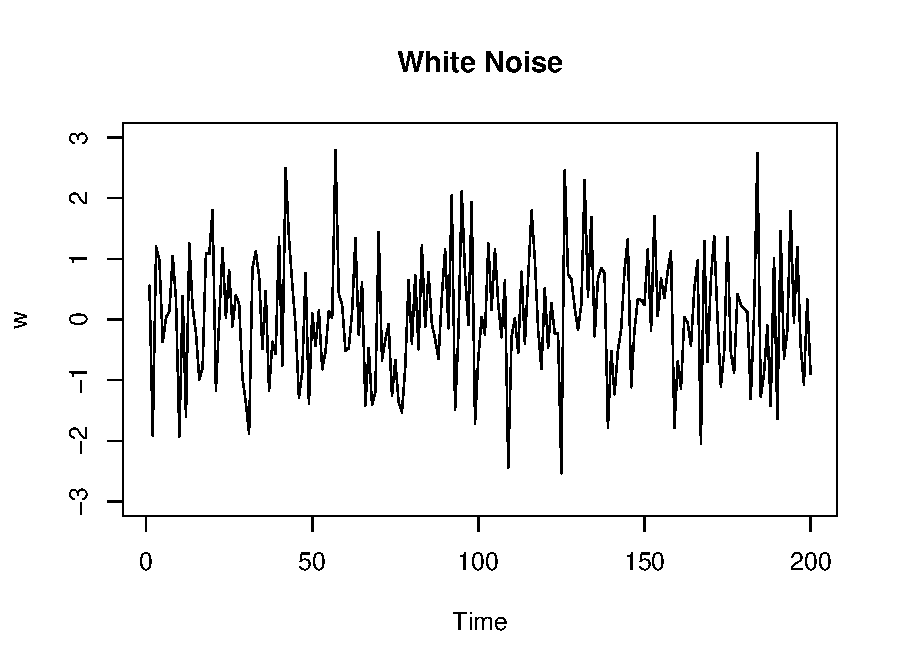
\includegraphics[scale=0.3]{white_noise.pdf}
%\end{figure}
%
%\end{frame}
\lstset{caption = Código R para generar Ruido blanco,framexleftmargin=5mm, frame=shadowbox, rulesepcolor=\color{green}}
\begin{lstlisting}[title={‘Código R para generar Ruido blanco’},basicstyle=\ttfamily]{}
set.seed(154)
w = rnorm(200,0,1)
plot.ts(w, ylim=c(-3,3), main="White Noise")
\end{lstlisting}\label{codigoRuidoBlanco}

\begin{figure}[H]
	\centering
	\textbf{Ruido blanco - White Noise}\par\medskip
	\fcolorbox{green}{blue}{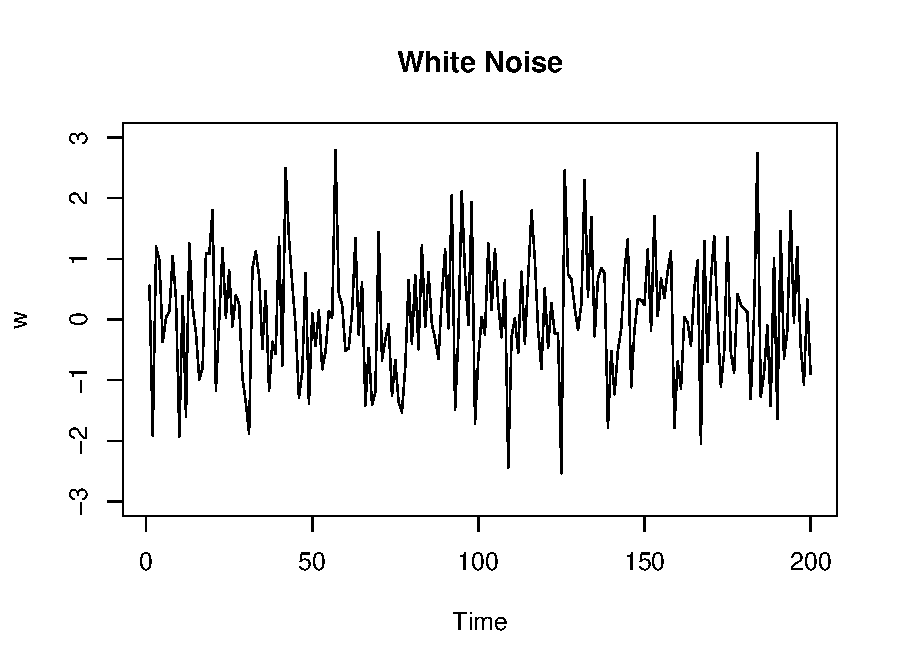
\includegraphics[width=\linewidth]{white_noise.pdf}}
	\caption{Ruido blanco - White Noise}\label{figura6}
\end{figure}

%---------------------------------------------------------
%---------------------Slide 21 --------------------------
%\begin{frame}
%\frametitle{Caminata Aleatoria - Random Walk}
\subsection{Caminata Aleatoria - Random Walk}

Un ejemplo simple para modelar una serie temporal estoc\'astica con tendencia (no estacionaria) es una caminata aleatoria con deriva (Random Walk with drift):

\begin{equation*}
x_t = \delta + x_{t-1} + \epsilon_t 
\end{equation*}

para $t = 1, 2,. . .$, con una condici\'on inicial $x_0 = 0$, y donde $\epsilon_t$ es ruido blanco. La constante $\delta$ se denomina deriva (drift), y cuando $\delta=0$, se llama simplemente una caminata aleatoria. El t\'ermino caminata aleatoria proviene del hecho de que, cuando $\delta=0$, el valor de la serie de tiempo en el tiempo $t$, es el valor de la serie en el tiempo $t - 1$ m\'as un movimiento completamente aleatorio determinado por $\epsilon_t$. 
%\end{frame}

%---------------------------------------------------------
%---------------------Slide 22 --------------------------
%\begin{frame}
%\frametitle{Caminata Aleatoria - Random Walk}

Tenga en cuenta que podemos reescribir la ecuaci\'on anterior como una suma acumulativa de las variables de ruido blanco. Es decir,

\begin{equation*}
x_t = \delta t + \sum_{j=1}^{t} \epsilon_t 
\end{equation*}

%\end{frame}
%---------------------------------------------------------
%---------------------Slide 23 --------------------------
%\begin{frame}
%\frametitle{Caminata Aleatoria - Random Walk}

%\only<1|handout:1>{
%	\begin{exampleblock}{C\'odigo en R}
%		set.seed(154) \\
%		w = rnorm(200,0,1) \\
%		x = cumsum(w) \\
%		wd = w + 0.2 \\
%		xd = cumsum(wd) \\
%		plot.ts(xd, ylim=c(-5,55), main=``random walk") \\
%		lines(x) \\
%		lines(0.2*(1:200), lty=``dashed") \\
%	\end{exampleblock}
%}
%\end{frame}
\lstset{caption = Código R para generar Caminata Aleatoria,framexleftmargin=5mm, frame=shadowbox, rulesepcolor=\color{green}}
\begin{lstlisting}[title={‘Código R para generar Caminata Aleatoria’},basicstyle=\ttfamily]{}
set.seed(154)
w = rnorm(200,0,1)
x = cumsum(w)
wd = w + 0.2
xd = cumsum(wd)
plot.ts(xd, ylim=c(-5,55), main="random walk")
lines(x)
lines(0.2*(1:200), lty="dashed")
\end{lstlisting}\label{codigoCaminataAleatoria}

%---------------------------------------------------------
%---------------------Slide 24 --------------------------
%\begin{frame}
%\frametitle{Caminata Aleatoria - Random Walk}

\begin{figure}[H]
	\centering
	\textbf{Caminata aleatoria}\par\medskip
	\fcolorbox{green}{blue}{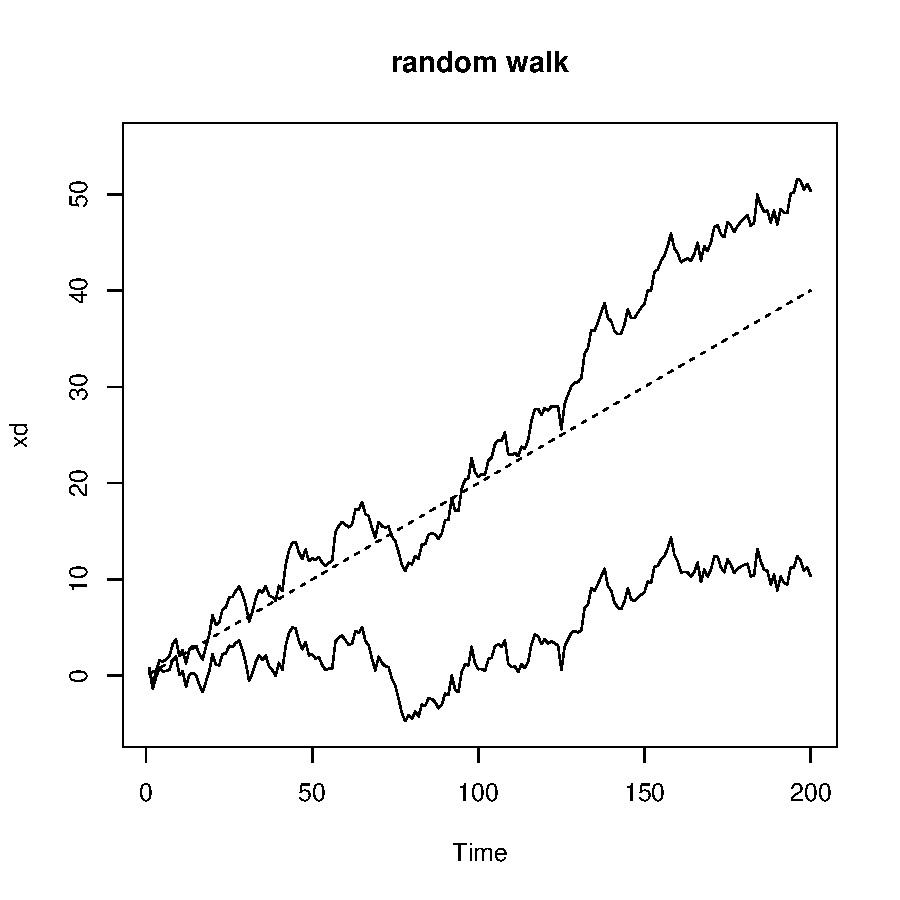
\includegraphics[width=\linewidth]{random_walk.pdf}}
%	\textbf{Random Walk}\par\medskip
%	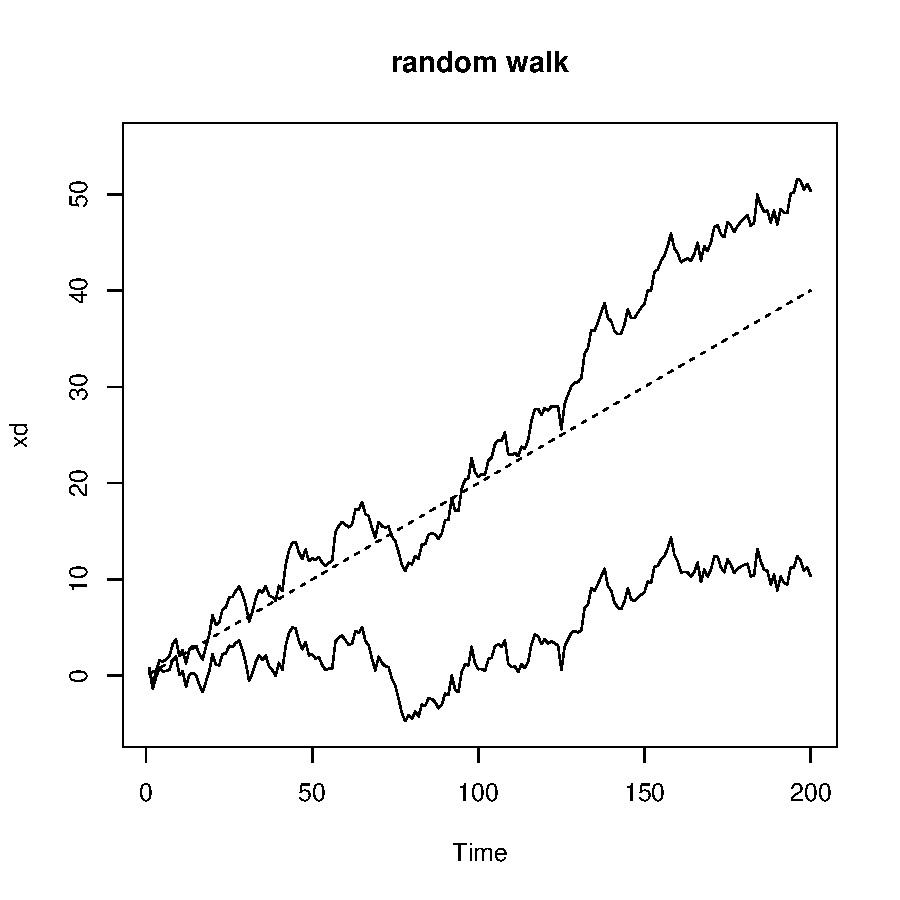
\includegraphics[scale=0.6]{random_walk.pdf}
	\caption{Caminata Aleatoria - Random walk, $\sigma_\epsilon$ = 1, with drift $\delta =0 .2$ (upper jagged line), without drift, $\delta = 0$ (lower jagged line), and a straight line with slope 0.2 (dashed line).}\label{figura7}
\end{figure}

%---------------------------------------------------------
%---------------------Slide 25 --------------------------
%\begin{frame}
%\frametitle{Promedios m\'oviles - Moving Averages}
\pagebreak\subsection{Promedios m\'oviles - Moving Averages}
Podr\'\i{}amos reemplazar la serie de ruido blanco $\epsilon_t$ por un promedio m\'ovil que suavice la serie. Por ejemplo, considere reemplazar $\epsilon_t$ por un promedio de su valor actual y sus vecinos inmediatos en el pasado y futuro. Es decir:

\begin{equation*}
v_t = 1/3 (\epsilon_{t-1} + \epsilon_t + \epsilon_{t+1})
\end{equation*}

Como veremos en el siguiente ejemplo, los promedios m\'oviles producen una versi\'on m\'as suave que la serie original, lo que refleja el hecho de que las oscilaciones m\'as lentas llegan a ser m\'as evidentes, y se eliminan algunas de las oscilaciones m\'as r\'apidas. 

%\end{frame}
%---------------------------------------------------------
%---------------------Slide 26 --------------------------
%\begin{frame}
%\frametitle{Promedios m\'oviles - Moving Averages}

%\only<1|handout:1>{
%	\begin{exampleblock}{C\'odigo en R}
%		w = rnorm(500,0,1) ; v = filter(w, sides=2, rep(1/3,3)) 
%		par(mfrow=c(2,1))\\
%		plot.ts(w, main=``white noise"); plot.ts(v, main=``moving average")\\
%	\end{exampleblock}
%}
\lstset{caption = Código R para generar Promedios móviles,framexleftmargin=5mm, frame=shadowbox, rulesepcolor=\color{green}}
\begin{lstlisting}[title={‘Código R para generar Moving Averages’},basicstyle=\ttfamily]{}
w = rnorm(500,0,1) ; v = filter(w, sides=2, rep(1/3,3))
par(mfrow=c(2,1))
plot.ts(w, main="white noise")
plot.ts(v, main="moving average")
\end{lstlisting}\label{movingAverage}
\begin{figure}[H]
	\centering
	\textbf{Medias móviles}\par\medskip
	\fcolorbox{green}{blue}{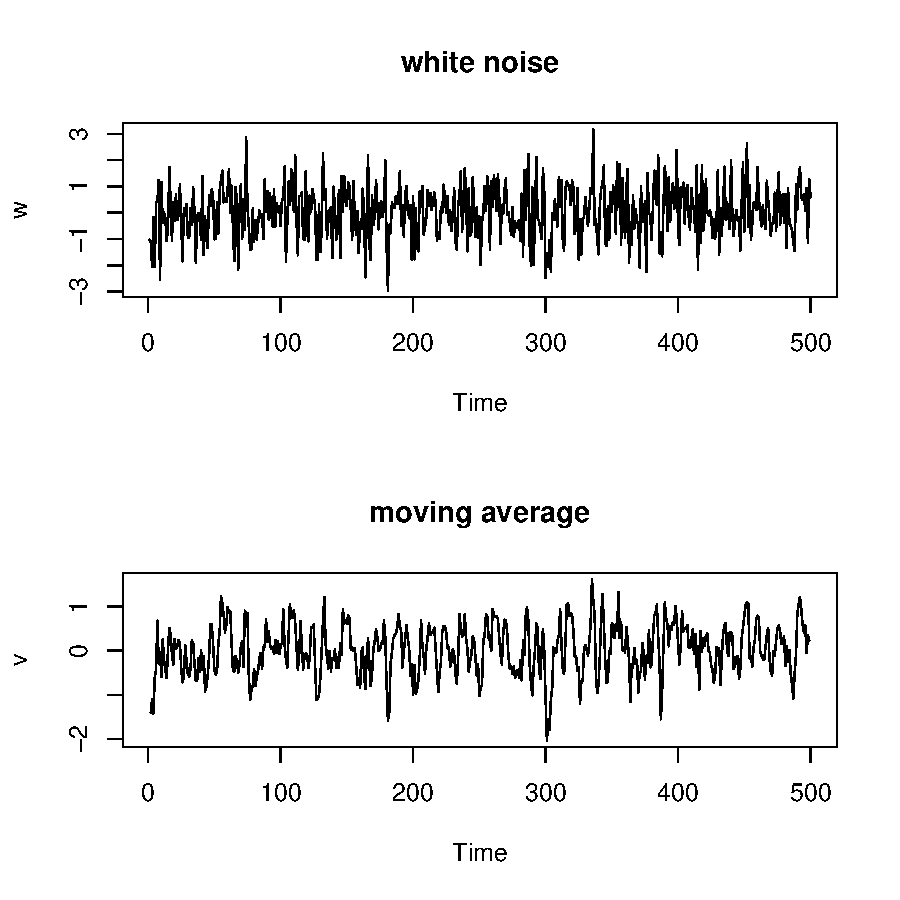
\includegraphics[width=\linewidth]{moving_average.pdf}}
%	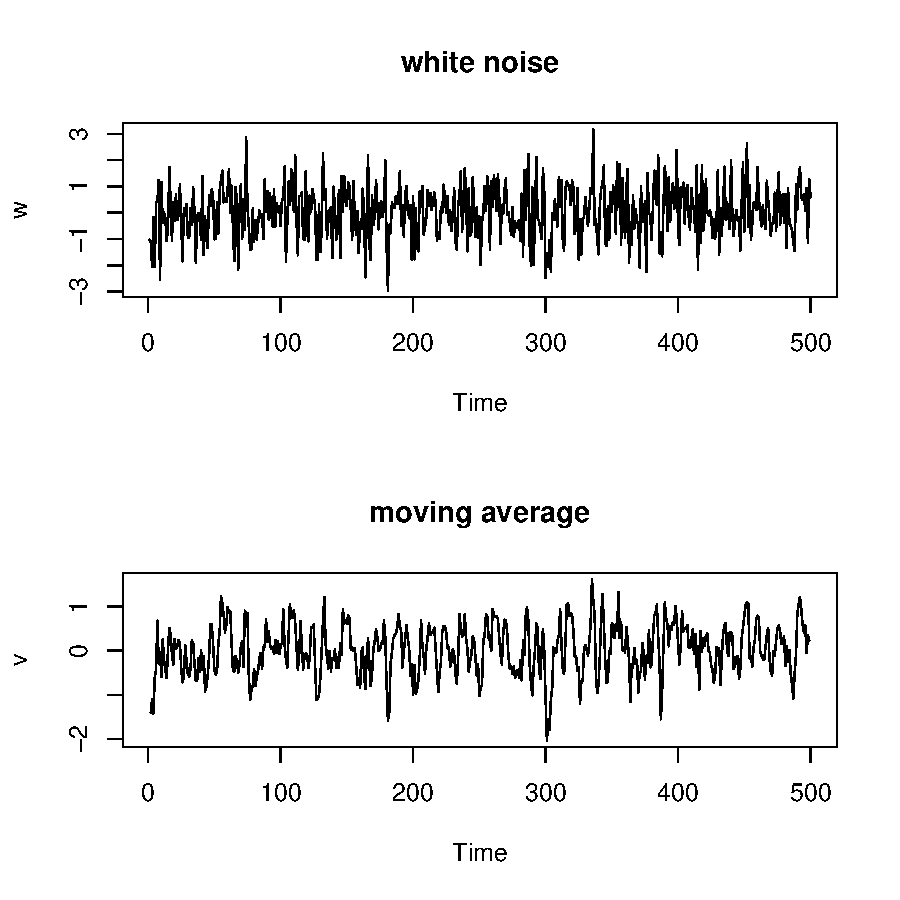
\includegraphics[scale=0.7]{moving_average.pdf}
	\caption{Promedios Móviles - Moving Averages}\label{figura8}
\end{figure}

%\end{frame}



%\end{frame}
%---------------------------------------------------------
%---------------------Slide 27 --------------------------
%\begin{frame}
%\frametitle{Autorregresiones - Autoregressions}
\subsection{Autorregresiones - Autoregressions}
Supongamos nuevamente que consideramos la serie de ruido blanco $w_t$ como entrada, y calculamos la salida usando una ecuaci\'on de segundo orden, es decir:

\begin{equation*}
x_t = x_{t-1} - 0.9 x_{t-2} + \epsilon_t
\end{equation*}

Esta ecuaci\'on representa una regresi\'on o predicci\'on del valor actual $x_t$ de una serie temporal en funci\'on de los dos valores anteriores de la serie, es por esto que utilizamos el nombre de autoregresi\'on.

%\end{frame}

%---------------------------------------------------------
%---------------------Slide 28 --------------------------
%\begin{frame}
%\frametitle{Autorregresiones - Autoregressions}

%\only<1|handout:1>{
%\begin{exampleblock}{C\'odigo en R}
%	w = rnorm(550,0,1) ; x = filter(w, filter=c(1,-.9), method= ``recursive")[-(1:50)]\\
%	plot.ts(x, main= ``autoregression")
%\end{exampleblock}
%}
\lstset{caption = Código R para generar Auto regresiones,framexleftmargin=5mm, frame=shadowbox, rulesepcolor=\color{green}}
\begin{lstlisting}[title={‘Código R para generar Autoregresions’},basicstyle=\ttfamily]{}
w = rnorm(550,0,1) ; 
x = filter(w, filter=c(1,-.9), method="recursive")[-(1:50)]
plot.ts(x, main= "autoregression")
\end{lstlisting}\label{autoregression}
\begin{figure}[H]
	\centering
	\textbf{Autorregresiones}\par\medskip
	\fcolorbox{green}{blue}{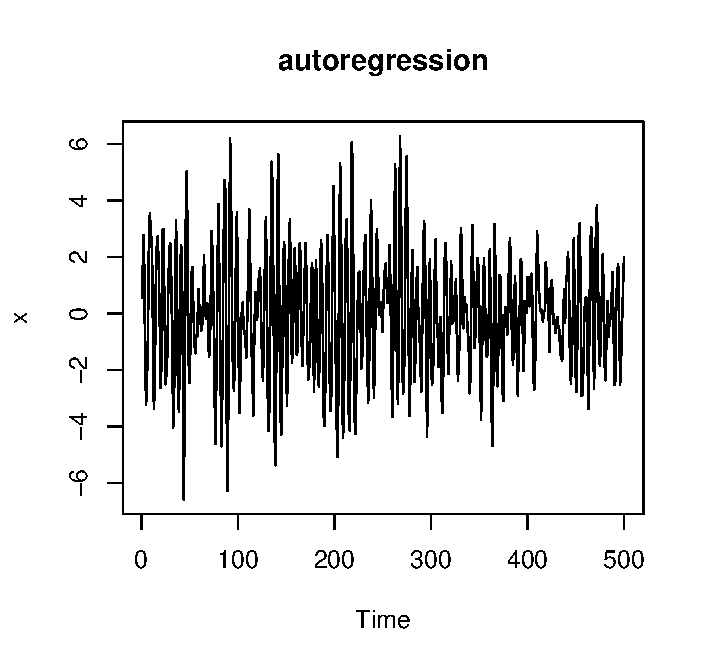
\includegraphics[width=\linewidth]{autoregression.pdf}}
%	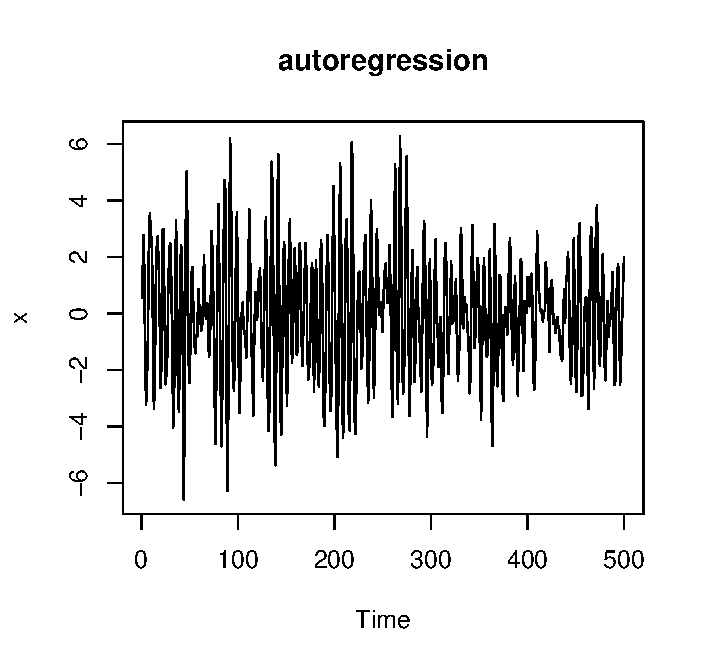
\includegraphics[scale=0.7]{autoregression.pdf}
	\caption{Autorregresiones - Autoregressions}\label{figura9}
\end{figure}

%---------------------------------------------------------
%---------------------Slide 29 --------------------------
\pagebreak\section{Descomposici\'on de las series de tiempo}
%	\begin{frame}
%	\frametitle{Descomposici\'on de las series de tiempo}	
Las series de tiempo usualmente se descomponen en:
	\begin{itemize}
		\item Una tendencia (trend) $T_t$. 
		\item Un componente estacional (seasonal) $S_t $.
		\item Un elemento irregular (irregular) $I_t$.
	\end{itemize}
	\vspace{5mm}
Por ejemplo:
	\begin{center}
		\vspace{3mm}
		$T_t=2+0.1 t$; \\
		\vspace{3mm}
		$S_t = 6.5 cos (\pi/60)$; \\
		\vspace{3mm}
		y $I_t\sim$ $N(\mu=0, \sigma^2=0.5)$. 
	\end{center}
%---------------------------------------------------------
%---------------------Slide 30 --------------------------
%\begin{frame}
%\frametitle{Descomposici\'on de las series de tiempo}
%
%\only<1|handout:1>{
%	\begin{exampleblock}{C\'odigo en R}
%		rm(list=ls())\\
%		$t = 2 + 0.1*1:500$\\
%		$s = 6.5*cos(pi*1:500/90)$\\
%		set.seed(154) \\
%		$i = rnorm(500,0,5)$\\
%		$plot.ts(s+t+i)$\\
%	\end{exampleblock}
%}
%\end{frame}
\lstset{caption = Código R para descomponer serie de tiempo,framexleftmargin=5mm, frame=shadowbox, rulesepcolor=\color{green}}
\begin{lstlisting}[title={‘Código R para descomponer serie de tiempo’},basicstyle=\ttfamily]{}
t = 2 + 0.1 * 1:500
s = 6.5 * cos(pi * 1:500/90)
set.seed(154)
i = rnorm(500, 0, 5)
plot.ts(s + t + i)
\end{lstlisting}\label{descomposicionTS}

%---------------------------------------------------------
%---------------------Slide 31 --------------------------
%\begin{frame}
%\frametitle{Descomposici\'on de las series de tiempo}
\begin{figure}[H]
	\centering
	\textbf{Componentes de uuna Serie de Tiempo}\par\medskip
	\fcolorbox{green}{blue}{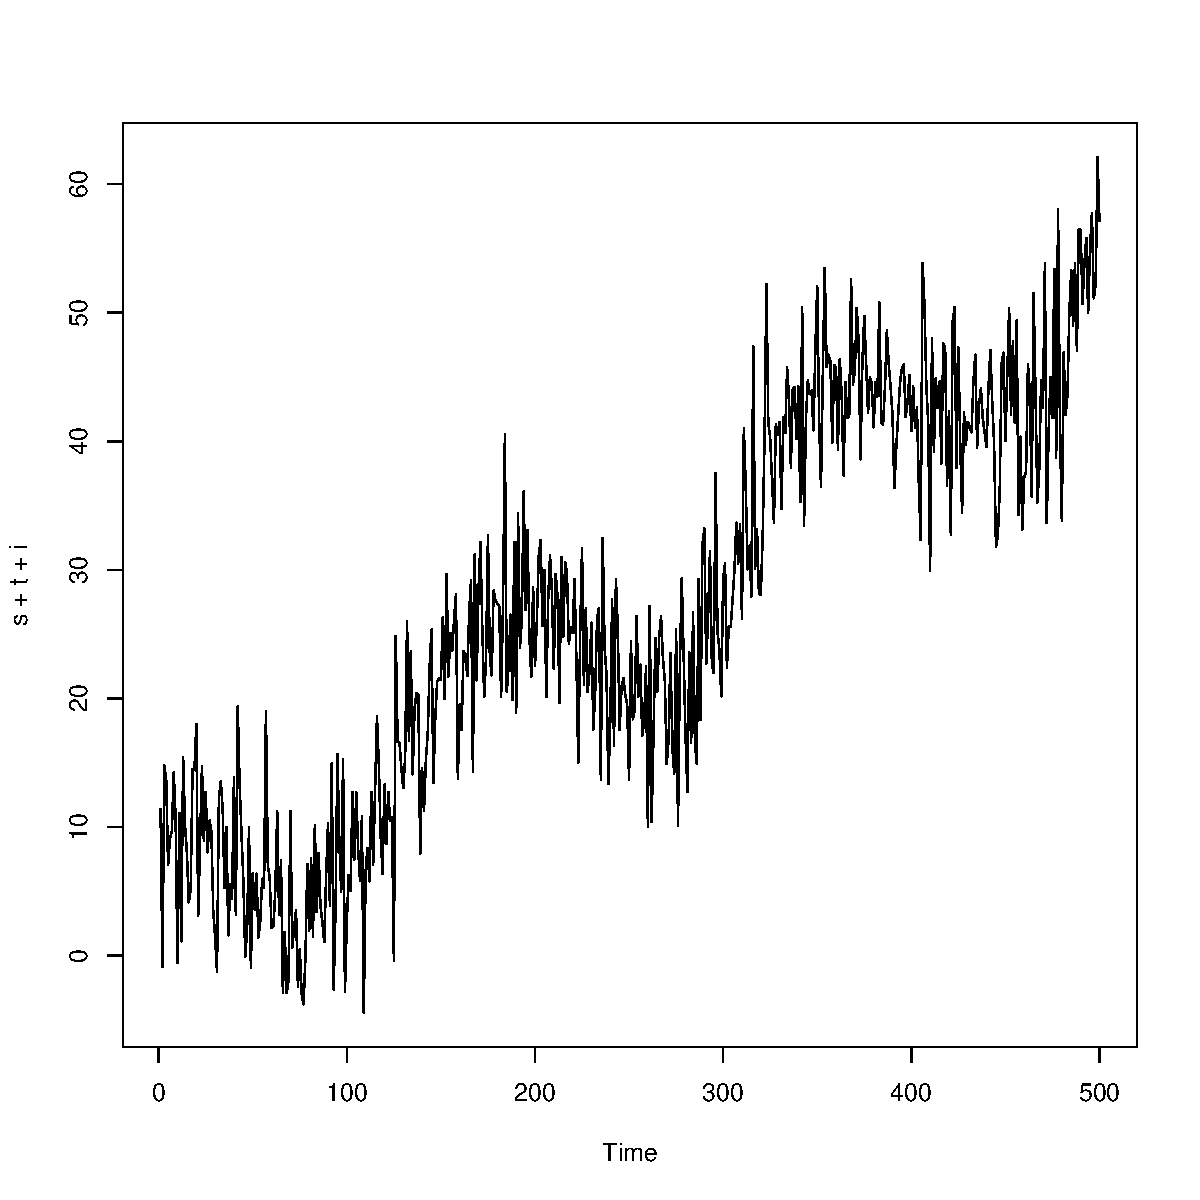
\includegraphics[width=\linewidth]{time_series.pdf}}
%	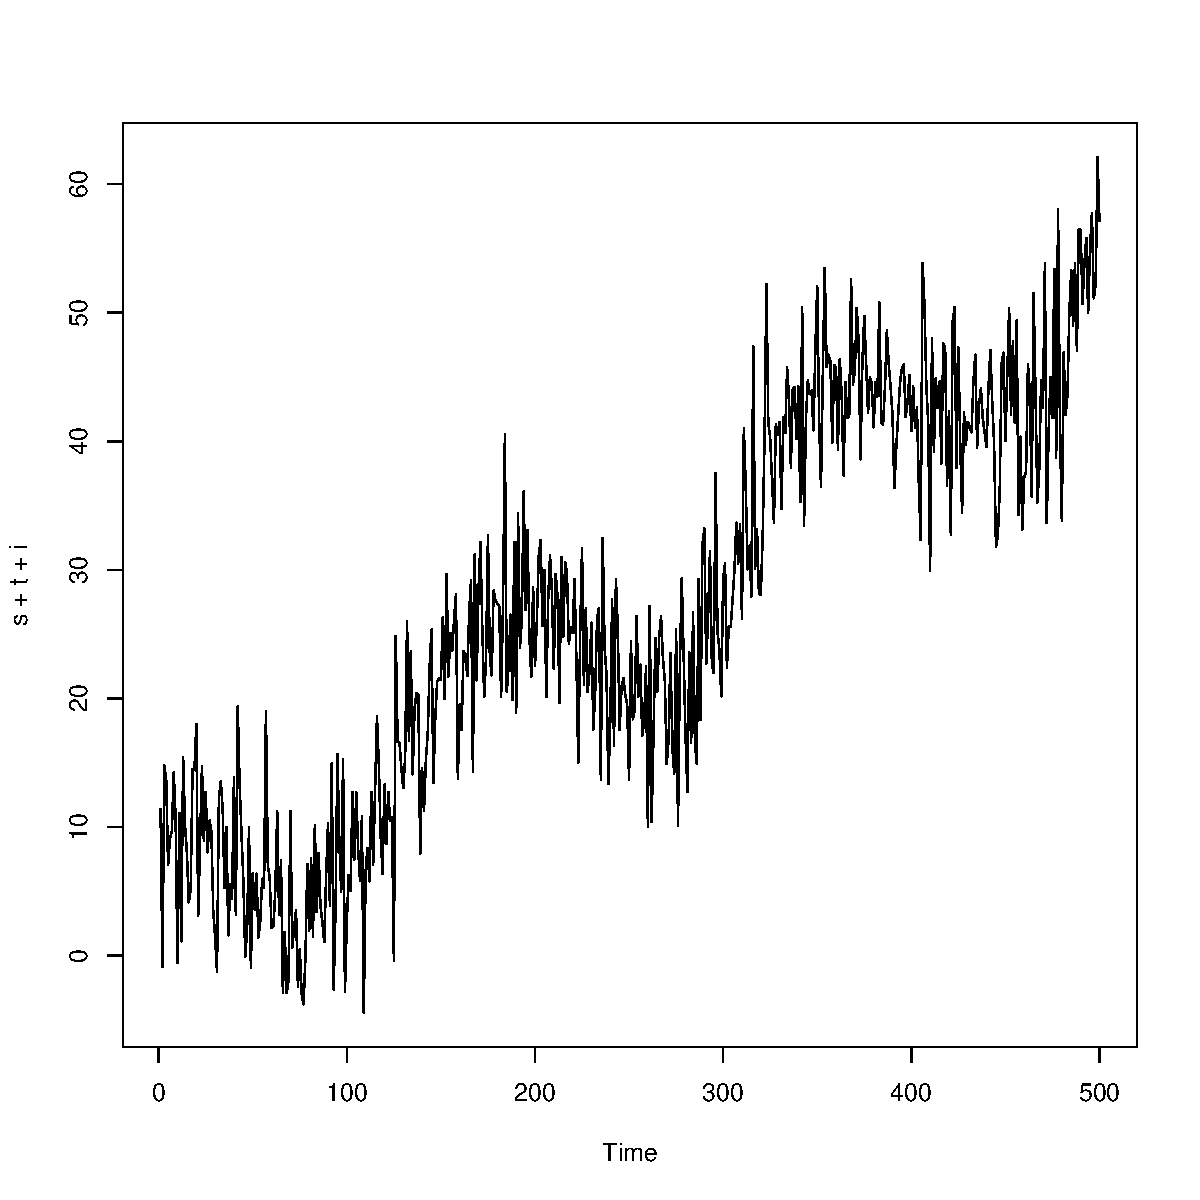
\includegraphics[scale=0.5]{time_series.pdf}
	\caption{Serie de tiempo con sus componentes T, S e I.}\label{figura10}
\end{figure}
%\end{frame}
%---------------------------------------------------------
%---------------------Slide 32 --------------------------
%\begin{frame}
%\frametitle{Descomposici\'on de las series de tiempo}

En general, las series de tiempo pueden contener uno o combinaci\'on de todos los elementos antes se\~nalados, ya sea de manera aditiva o multiplicativa:

\begin{equation*}
x_t = T_t + S_t + I_t
\end{equation*}

\begin{equation*}
x_t = T_t * S_t * I_t
\end{equation*}

\begin{itemize}
\item La primera especificaci\'on se caracteriza por tener cada componente de forma independiente, lo que posibilita descomponer la serie en una suma de los tres factores.
\item  La segunda, por otra parte, surge cuando la tendencia $(T_t)$, estacionalidad $(S_t)$, y irregularidad $(I_t)$ son dependientes entre si.
\end{itemize}

%\end{frame}

%---------------------------------------------------------
%---------------------Slide 33 --------------------------
%\begin{frame}
%\frametitle{Descomposici\'on de las series de tiempo}

En general, la tendencia cambia la media de la serie, mientras que el componente estacional posee un patr\'on que se repite, por ejemplo de manera mensual o trimestral. El componente irregular a pesar de no tener un patr\'on bien definido, puede ser pronosticada, de hecho, los pron\'osticos usan correlaciones con el componente irregular para realizar sus pron\'osticos. En per\'\i{}odos m\'as largos sin embargo, el componente irregular exhibe una tendencia de reversi\'on a cero.\\
El pron\'ostico de series de tiempo pretende entonces predecir cada uno de \'estos componentes de manera individual. Como vimos, el pron\'ostico global de la series de tiempo agrupa de forma aditiva o multiplicativa cada uno de dichos componentes.

%---------------------------------------------------------
%---------------------Slide 34 --------------------------
%\begin{frame}
%\frametitle{Descomposici\'on Tendencia\\
\subsection{Descomposici\'on Tendencia - Filtro Hodrick -Prescott}

\begin{itemize}
	\item En econom\'\i{}a, el filtro Hodrick-Prescott (HP) permite separar para $x_t$  los componentes tendencial y c\'\i{}clico.
	\item Este m\'etodo consiste en obtener una serie suavizada $S_t$ a partir de la original $x_t$, mediante una soluci\'on al problema de optimizaci\'on sugerido en la siguiente ecuaci\'on. Una vez resuelto, permite estimar tanto el ciclo como la tendencia de la serie.
\end{itemize}

\begin{equation*}
min \sum_{t=1}^{n} \left(x_t -S_t\right)^2 + \lambda \sum_{t=2}^{n-1} \left[ \left(S_{t+1}-S_t\right)-\left(S_t-S_{t-1}\right)\right]^2
\end{equation*}

\begin{itemize}
	\item Los valores sugeridos para $\lambda$ dependen de la periodicidad de $x_t$, y son: 14400 (mensual), 1600 (trimestral) y 100 (anual). Por otra parte, una vez obtenido el componente c\'\i{}clico $ \left(x_t -S_t\right)$, a partir del filtro HP, puede ser interpretada como la brecha existente entre su valor real $x_t$ y potencial $S_t$.
\end{itemize}

%---------------------------------------------------------
%---------------------Slide 35 --------------------------
%\begin{frame}
%\frametitle{Descomposici\'on componente estacional\\ 	Transformaciones de Diferencias}
\subsection{Descomposici\'on componente estacional - Transformaciones de Diferencias}

La transformaciones de diferencias se usan para capturar el componente estacional de la serie:

Una primera diferencia es definida como:

\begin{equation*}
\triangle x_t = (x_t - x_{t-1})
\end{equation*}

An\'alogamente, la segunda diferencia es definida como:

\begin{equation*}
\triangle^2x_t = (x_t - x_{t-1})-(x_{t-1} - x_{t-2})
\end{equation*}
Anteriormente vimos que la primera diferencia del logaritmo, se pod\'\i{}a interpretar como el cambio porcentual de la variable, logrando la simetr\'\i{}a del precio de las acciones.

%---------------------------------------------------------

%---------------------Slide 36 --------------------------
%\begin{frame}
%\frametitle{Descomposici\'on componente estacional\\
%	Variables Dummy}
\subsection{Descomposici\'on componente estacional - Variables Dummy}
Una variable dummy, D, es una variable binaria que toma la siguiente forma:

\begin{itemize}
	\item D=1  si la observaci\'on tiene caracter\'\i{}sticas espec\'\i{}ficas.
	\item D=0 si no las tiene.
\end{itemize}

Por ejemplo:

\begin{equation*}
x_t  = \beta_0 + \beta_1 z_t + \beta_2 D + \beta_3 D z_t
\end{equation*}

\begin{equation*}
D=1 => x_t  = (\beta_0 + \beta_2) + (\beta_1 + \beta_3) z_t
\end{equation*}

\begin{equation*}
D=0 => x_t  = \beta_0 + \beta_1 z_t
\end{equation*}

Las variables dummy pueden ser usadas para cambiar la pendiente y/o intercepto en un modelo lineal, lo cual permite capturar la estacionalidad en la serie, por ejemplo con variables dummys por trimestre o temporada.
%---------------------------------------------------------
%---------------------Slide 37 --------------------------
%\begin{section}{Medidas de dependencia}
%	\begin{frame}
%	\frametitle{Medidas de dependencia}
\pagebreak\section{Medidas de dependencia}
	Como vimos anteriormente, una serie de tiempo puede ser vista como una colecci\'on de n variables aleatorias en puntos de tiempo enteros arbitrarios $t_1, t_2,\cdots, t_n$, para cualquier entero positivo se cuenta con una funci\'on de distribuci\'on conjunta, evaluada como la probabilidad que los valores de las series sean conjuntamente menores que n constantes, $c_1, c_2,\cdots, c_n$, i.e.:
	\begin{equation*}
	F(c_1, c_2,\cdots, c_n) =  P(x_{t_1},\le c_1, x_{t_2} 	\le c_2,\cdots x_{t_n} \le c_n)
	\end{equation*}

%\end{frame}
%---------------------------------------------------------
%---------------------Slide 38 --------------------------
%\begin{frame}
%\frametitle{Medidas de dependencia}

Desafortunadamente, la funci\'on de distribuci\'on multinomial no puede usualmente ser escrita f\'acilmente a menos que las variables sean conjuntamente normales, en cual caso la densidad conjunta presenta la forma:
\begin{equation*}
f(\textbf{x}) = (2\pi)^{-2/n}\mid\Gamma\mid^{-1/2} exp \{ -1/2  (\textbf{x} - \mu)' \Gamma^{-1}\ (\textbf{x} - \mu)\}
\end{equation*}

donde $\mid\cdot\mid$ indica determinante y $\Gamma$ la matriz de covarianza.\\
Aunque la funci\'on de distribuci\'on conjunta permite describir la data completamente, su manipulaci\'on es muy compleja, y su despliegue gr\'afico imposible.
%\end{frame}
%---------------------------------------------------------
%---------------------Slide 39 --------------------------
%\begin{frame}
%\frametitle{Medidas de dependencia}

Las funciones de distribuci\'on marginales:
\begin{equation*}
F_t(x) = P\{x_t \le x\}
\end{equation*}

o la correspondiente funci\'on de densidad marginal:\\
\begin{equation*}
f_t(x) = \frac{\partial F_t(x)}{\partial x} 
\end{equation*}
\\
Cuando \'estas existen, proveen informaci\'on valiosa para examinar el comportamiento marginal de la serie.
\\
Si $x_t$ es Gausiana con media $\mu_t$ y varianza $\sigma_t^2$, $x_t$ $\sim$ $N(\mu_t,\sigma_t^2)$, la densidad marginal esta dada por:

\begin{equation*}
f_t(x) = \frac{1}{\sigma_t \sqrt{2 \pi}} exp  ( -  \frac{1}{2 \sigma_t^2}  (\textbf{x} - \mu_t)^2 )
\end{equation*}
%\end{frame}

%---------------------------------------------------------
%---------------------Slide 40 --------------------------
%\begin{frame}
%\frametitle{Medidas de dependencia}

La funci\'on de media, conocida en estad\'\i{}stica como el primer momento central, est\'a definida como:
\vspace{5mm}

%\only<1|handout:1>{
%\begin{block}{Definici\'on: Funci\'on de Media}
%	\begin{equation*}
%	\mu_{xt} = E(x_t)= \int^{+\infty}_{-\infty} x f_t(x)dx
%	\end{equation*}
%\end{block}
%}
%\section{Definition}
\begin{definition}\label{def:def1}
	\textbf{Definici\'on: Funci\'on de Media:}
	\begin{equation*}
	\mu_{xt} = E(x_t)= \int^{+\infty}_{-\infty} x f_t(x)dx
	\end{equation*} 

\end{definition}

Si existe, E denota el operador de valor esperado.

%\end{frame}

%---------------------------------------------------------
%---------------------Slide 41 --------------------------
%\begin{frame}
%\frametitle{Medidas de dependencia}

La funci\'on de autocovarianza, conocida en estad\'\i{}stica como el segundo momento central, est\'a definida como:
\vspace{5mm}

%\only<1|handout:1>{
%\begin{block}{Definici\'on: Funci\'on de Autocovarianza}
%\begin{equation*}
%\gamma_{x}(s,t) = cov(x_s, x_t) = E[(x_s - \mu_s)(x_t - \mu_t)] 
%\end{equation*}
%\end{block}
%}
%\section{Definition}
\begin{definition}\label{def:def2}
	\textbf{Definici\'on: Funci\'on de Autocovarianza:} 
	\begin{equation*}
	\gamma_{x}(s,t) = cov(x_s, x_t) = E[(x_s - \mu_s)(x_t - \mu_t)] 
	\end{equation*}
\end{definition}

En este caso, $\gamma_{x}(s,t) = \gamma_{x}(t,s)$ para todos los puntos de $s$ y $t$. Si $\gamma(s,t)=0$ podemos asegurar que $x_s$ y $x_t$ no est\'an linealmente relacionadas. Por otro lado, si $x_s$ y $x_t$  son adem\'as normales bivariadas podemos asegurar que son independientes.
\\
Por \'ultimo, es claro que si $s = t$, la autocovarianza se reduce a la varianza
%\only<1|handout:1>{
%\begin{block}{Definici\'on: Funci\'on de Varianza}
%\begin{equation*}
%\gamma_{x}(t,t) = E[(x_t - \mu_t)^2] = var(x_t) 
%\end{equation*}
%\end{block}
%}
%\section{Definition}
\begin{definition}\label{def:def3}
	\textbf{Definici\'on: Funci\'on de Varianza:}
	\begin{equation*}
	\gamma_{x}(t,t) = E[(x_t - \mu_t)^2] = var(x_t) 
	\end{equation*} 
\end{definition} 



%\end{frame}

%---------------------------------------------------------
%---------------------Slide 42 --------------------------
%\begin{frame}
%\frametitle{Medidas de dependencia}

La Funci\'on de Autocorrelaci\'on, denotada por ACF (autocorrelation function),  mide la predictibilidad lineal de la serie en el tiempo t. Es decir, predecimos $x_t$, utilizando s\'olo el valor $x_s$. Suponiendo que ambas series tienen varianzas finitas, tenemos la siguiente definici\'on:

\vspace{5mm}

%\only<1|handout:1>{
%\begin{block}{Definici\'on: Funci\'on de Autocorrelaci\'on}
%\begin{equation*}
%\rho(s,t) = \frac{\gamma(s,t)}{ \sqrt{\gamma(s,s) \gamma(t,t)}}
%\end{equation*}
%\end{block}
%}
%\section{Definition}
\begin{definition}\label{def:def4}
	\textbf{Definici\'on: Funci\'on de Autocorrelaci\'on:} 
	\begin{equation*}
	\rho(s,t) = \frac{\gamma(s,t)}{ \sqrt{\gamma(s,s) \gamma(t,t)}}
	\end{equation*}
\end{definition} 

Se puede demostrar f\'acilmente que $-1 \le \rho(s,t) \le 1$. Si podemos predecir $x_t$ perfectamente a partir de $x_s$ a trav\'es de una relaci\'on lineal, $x_t = \beta_0 + \beta_1 x_s$, entonces la correlaci\'on ser\'a $+1$ cuando $\beta_1 > 0$, y $-1$ cuando $\beta_1 < 0$. \\
Por lo tanto, tenemos una medida aproximada de la capacidad de predecir la serie en el tiempo $t$ desde el valor en el tiempo $s$.

%\end{frame}

%---------------------------------------------------------
%---------------------Slide 43 --------------------------
%\begin{frame}
%\frametitle{Medidas de dependencia}

La funci\'on de covarianza cruzada entre dos series, $x_t$ e $y_t$, viene dada por:
\vspace{5mm}

%\only<1|handout:1>{
%\begin{block}{Definici\'on: Funci\'on de Covarianza Cruzada}
%\begin{equation*}
%\gamma_{xy} (s, t) = cov (x_s, y_t) = E [(x_s -\mu_{xs}) (y_t - \mu_{yt})].
%\end{equation*}
%\end{block}
%}
%\section{Definition}
\begin{definition}\label{def:def5}
	\textbf{Definici\'on: Funci\'on de Covarianza Cruzada:}
\begin{equation*}
\gamma_{xy} (s, t) = cov (x_s, y_t) = E [(x_s -\mu_{xs}) (y_t - \mu_{yt})].
\end{equation*}
\end{definition}
La funci\'on de correlaci\'on cruzada (CCF por su sigla en ingl\'es cross-correlation function) est\'a dada por:
\vspace{5mm}

%\only<1|handout:1>{
%\begin{block}{Definici\'on: Funci\'on de Correlaci\'on Cruzada}
%\begin{equation*}
%\rho_{xy} (s, t) = \frac{\gamma_{xy}(s,t)}{ \sqrt{\gamma_x(s,s) \gamma_y(t,t)}}
%\end{equation*}
%\end{block}
%}
%\section{Definition}
\begin{definition}\label{def:def6}
\textbf{Funci\'on de Correlaci\'on Cruzada:}
\begin{equation*}
\rho_{xy} (s, t) = \frac{\gamma_{xy}(s,t)}{ \sqrt{\gamma_x(s,s) \gamma_y(t,t)}}
\end{equation*}

\end{definition} 

%\end{frame}
%---------------------------------------------------------
%---------------------Slide 44 --------------------------
%\begin{frame}
%\frametitle{Medidas de dependencia}

Podemos extender f\'acilmente las formulaciones anteriores al caso de m\'as de dos series, por ejemplo, $x_{t1}, x_{t2},\cdots, x_{tr}$; es decir, series temporales multivariantes con $r$ componentes. Por ejemplo, la extensi\'on de (1.10) para el caso de covarianza cruzada ser\'\i{}a:

\begin{equation*}
\gamma_{xy} (j, k) = cov (x_{sj}, y_{sk}) = E [(x_s -\mu_{xs}) (y_{tj} - \mu_{y_{tk}})].
\end{equation*}

%---------------------------------------------------------
%---------------------Slide 45 --------------------------
%\begin{section}{Estacionaridad}
%	\begin{frame}
%	\frametitle{Estacionaridad}
%	
%	\only<1|handout:1>{
%		\begin{block}{Definici\'on: Estacionaridad estricta}
%			Una serie de tiempo es estrictamente estacionaria (strictly stationary) si el comportamiento probabil\'\i{}stico de cada conjunto de valores $\{x_{t_1}, x_{t_2}, ..., x_{t_k}\}$ es id\'entico al del mismo conjunto desplazado en el tiempo, es decir $\{x_{t_1+h} , x_{t_2+h}, ..., x_{t_k + h}\}$.\\
%		\end{block}
%	}
\section{Estacionaridad}
\begin{definition}\label{def:def7}
	\textbf{Definici\'on: Estacionaridad estricta:}
Una serie de tiempo es estrictamente estacionaria (strictly stationary) si el comportamiento probabil\'\i{}stico de cada conjunto de valores $\{x_{t_1}, x_{t_2}, ..., x_{t_k}\}$ es id\'entico al del mismo conjunto desplazado en el tiempo, es decir $\{x_{t_1+h} , x_{t_2+h}, ..., x_{t_k + h}\}$.\\
\end{definition} 
En otras palabras:
	
	\begin{equation*}
	P(x_{t_1},\le c_1, \cdots x_{t_k} \le c_k) = P(x_{t_1}+h,\le c_1\cdots x_{t_k+h} \le c_k)
	\end{equation*}
	
	para todos los $k = 1,2, ...$, todos los per\'\i{}odos $t_1, t_2, ..., t_k$, todos los n\'umeros $c_1, c_2, ..., c_k$, y todos los desplazamientos de tiempo $h = 0, \pm 1, \pm 2 , ....$
	
%\end{frame}
%---------------------------------------------------------
%---------------------Slide 46 --------------------------
%\begin{frame}
%\frametitle{Estacionaridad}

Si una serie de tiempo es estrictamente estacionaria, entonces todas las funciones de distribuci\'on multivariante para subconjuntos de variables, deben ser iguales con sus contrapartes en el conjunto desplazado. Por ejemplo, cuando $k = 1$:

\begin{equation*}
P \{x_s \le c\} = P \{x_t \le c\}
\end{equation*}

para cualquier punto de tiempo $s$ y $t$. \\

Cuando $k=2$ tenemos:

\begin{equation*}
P \{x_s \le c_1, x_t \le  c_2\} = P \{x_{s+h} \le c_1, x_{t+h} \le  c_2\} 
\end{equation*}

Para cualquier punto de $s$, $t$ y $h$. Si la funci\'on de varianza existe, entonces: $\gamma(s,t)=\gamma(s+h,t+h)$

En este contexto, ?`es un proceso random walk with drift estr\'\i{}ctamente estacionario?\\

%\end{frame}

%\end{section}
%---------------------------------------------------------
%---------------------Slide 47 --------------------------
%\begin{frame}
%\frametitle{Estacionaridad}
%
%\only<1|handout:1>{
%	\begin{block}{Definici\'on: Estacionaridad d\'ebil}
%		Una serie de tiempo $x_t$ d\'ebilmente estacionaria (weakly stationary) es un proceso de varianza finita tal que:
%		\begin{itemize}
%			\item (i) la funci\'on de valor medio, $\mu_t$, es constante y no depende del tiempo $t$, y
%			\item (ii) la funci\'on de autocovarianza, $\gamma(s, t)$, depende de s y t s\'olo a trav\'es de su diferencia $| s - t |$.
%		\end{itemize}
%	\end{block}
%}
\begin{definition}\label{def:def8}
	\textbf{Definici\'on: Estacionaridad d\'ebil:} Una serie de tiempo $x_t$ d\'ebilmente estacionaria (weakly stationary) es un proceso de varianza finita tal que:
			\begin{itemize}
				\item (i) la funci\'on de valor medio, $\mu_t$, es constante y no depende del tiempo $t$, y
				\item (ii) la funci\'on de autocovarianza, $\gamma(s, t)$, depende de s y t s\'olo a trav\'es de su diferencia $| s - t |$.
			\end{itemize}
\end{definition} 

De ahora en adelante, usaremos el t\'ermino estacionario para significar d\'ebilmente estacionario; si un proceso es estacionario en sentido estricto, utilizaremos el t\'ermino estrictamente estacionario.\\
Un caso importante en el que la estacionariedad implica una estacionariedad estricta es si la serie es gaussiana (es decir, todas las distribuciones finitas de la serie son gaussianas). 

%\end{frame}
%---------------------------------------------------------
%---------------------Slide 48 --------------------------
%\begin{section}{Modelos de regresi\'on lineal m\'ultiple en series de tiempo}
%	\begin{frame}
%	\frametitle{Modelos de regresi\'on lineal m\'ultiple en series de tiempo}
\section{Modelos de regresi\'on lineal m\'ultiple en series de tiempo}
	A continuaci\'on introducimos (recordamos) el modelo cl\'asico de regresi\'on lineal.
	\begin{itemize}
		\item Sea $\mathbf{X}$ una matriz de $n\times k$ entradas donde se tienen
		$n$ observaciones para $k$ independientes variables.
		\item Sea $\mathbf{Y}$ un vector de $n$ observaciones de la variable dependiente.
		\item Es posible proponer un modelo de estimaci\'on lineal que relaciona las
		variables $\mathbf{X}$ y la variable $\mathbf{Y}$:
	\end{itemize}
	
	\[
	\begin{bmatrix}Y_{1}\\
	Y_{2}\\
	\vdots\\
	Y_{n}
	\end{bmatrix}=\begin{bmatrix} 1 & X_{11} & X_{21} & \cdots & X_{k1}\\
	1 & X_{12} & X_{22} & \cdots & X_{k2}\\
	\vdots & \vdots & \ddots & \vdots\\
	1 & X_{1n} & X_{2n} & \cdots & X_{kn}
	\end{bmatrix}\begin{bmatrix}\beta_{0}\\
	\beta_{1}\\
	\vdots\\
	\beta_{n}
	\end{bmatrix}+\begin{bmatrix}\epsilon_{1}\\
	\epsilon_{2}\\
	\vdots\\
	\epsilon_{n}
	\end{bmatrix}
	\]
	
%\end{frame}
%---------------------------------------------------------
%---------------------Slide 49 --------------------------
%\begin{frame}
%\frametitle{Modelos de regresi\'on lineal m\'ultiple en series de tiempo}

El modelo tambi\'en puede ser escrito de forma compacta como:

\[
\mathbf{Y}=\mathbf{X}\mathbf{\beta}+\mathbf{\epsilon}
\]

Vemos que este modelo presenta componentes sistem\'aticos (deterministicos) ($\mathbf{X\beta})$ 
y estoc\'asticos ($\epsilon$).\\
Lo que se busca es determinar los coeficientes $\beta_{i}$ que relacionen linealmente a la variables $X_{i}$ e $Y$. 
Para esto utilizamos el m\'etodo de m\'\i{}nimos cuadrados ordinarios (MCO, tambi\'en conocido como OLS por su sigla en ingl\'es: ordinary least square)
El criterio de m\'\i{}nimos cuadrados busca minimizar la suma de los cuadrados
de los residuos ($\sum e_{i}^{2}$).

%\end{frame}
%---------------------------------------------------------

%---------------------Slide 50 --------------------------
%\begin{frame}
%\frametitle{Modelos de regresi\'on lineal m\'ultiple en series de tiempo}

A continuaci\'on revisamos la derivaci\'on del m\'etodo de MCO. Primero, el vector de residuos se puede obtener como:

\[
\mathbf{e}=\mathbf{Y}-\mathbf{X\hat{\beta}}
\]

donde \textbf{$\hat{\beta}$} representa el estimador del vector $\mathbf{\beta}$.

Por lo que la sumatoria del cuadrado de los errores ser\'a:

\[
\mathbf{e'e}=\begin{bmatrix}e_{1} & e_{2} & \ldots & e_{n}\end{bmatrix}\begin{bmatrix}e_{1}\\
e_{2}\\
\vdots\\
e_{n}
\end{bmatrix}=\begin{bmatrix}e_{1}^{2}+e_{2}^{2}+\ldots+e_{n}^{2}\end{bmatrix}
\]

%\end{frame}
%---------------------------------------------------------
%---------------------Slide 51 --------------------------
%\begin{frame}
%\frametitle{Modelos de regresi\'on lineal m\'ultiple en series de tiempo}

Por otro lado, puede escribirse tambi\'en como:

\begin{eqnarray*}
	\mathbf{e'e} & = & \left(\mathbf{Y-X\hat{\beta}}\right)'\left(\mathbf{Y-X\hat{\beta}}\right)\\
	& = & \mathbf{Y'Y}-\mathbf{\hat{\beta}'X'Y}-\mathbf{Y'X\hat{\beta}}+\mathbf{\hat{\beta}'X'X\hat{\beta}}\\
	& = & \mathbf{Y'Y}-\mathbf{2\hat{\beta}'X'Y}+\mathbf{\hat{\beta}'X'X\hat{\beta}}
\end{eqnarray*}

Para minimizar el cuadrado de los residuos recurrimos al c\'alculo diferencial:

\[
\frac{\partial(\mathbf{e'e})}{\partial\mathbf{\hat{\beta}}}=-2\mathbf{X'Y}+2\mathbf{X'X\hat{\beta}}=0
\]

Luego $\mathbf{\hat{\beta}}$ sera un m\'\i{}nimo de \textbf{$\mathbf{e'e}$}
si la segunda derivada es positiva o equivalentemente $\mathbf{X}$
es definida positiva.

%\end{frame}
%---------------------------------------------------------
%---------------------Slide 52 --------------------------
%\begin{frame}
%\frametitle{Modelos de regresi\'on lineal m\'ultiple en series de tiempo}


De la expresi\'on anterior obtenemos:

\[
\mathbf{X'X\hat{\beta}}=\mathbf{X'Y}
\]

Finalmente, multiplicando por $(\mathbf{X'X})^{-1}$ a ambos lados, obtenemos $\hat\beta$:

\[
\mathbf{\hat\beta}=(\mathbf{X'X})^{-1}\mathbf{X'Y}
\]
\\
La facilidad de c\'alculo del MCO ha influido en su popularidad. Los estimadores se obtienen a trav\'es de sencillas operaciones de matrices 

%\end{frame}
%---------------------------------------------------------
%---------------------Slide 53 --------------------------
%\begin{frame}
%\frametitle{Propiedades de los estimadores de MC}
\subsection{Propiedades de los estimadores de MC}
La estimaci\'on de los MCO es la mejor estimaci\'on lineal no sesgada (BLUE, best linear unbiased estimators). La prueba de esta proposici\'on es provista por el teorema Gauss-Markov.

\begin{enumerate}
	\item (i) No sesgado: $E(\hat{\beta}) = \beta$, es decir el valor esperado de el estimador es el verdadero valor de el par\'ametro desconocido.
	\item (ii) Mejor: m\'\i{}nima varianza.
\end{enumerate}

%\end{frame}
%---------------------------------------------------------
%---------------------Slide 54 --------------------------
%\begin{frame}
%\frametitle{Teorema Gauss-Markov}

%\only<1|handout:1>{
%	\begin{block}{Supuestos}
%		\begin{enumerate}
%			\item Existe una relaci\'on lineal entre $\mathbf{X}$ e \textbf{$\mathbf{Y}$}
%			\item No existe multicolinealidad (\textbf{X} es linealmente independiente)
%			\item $E(\mathbf{\epsilon}|\mathbf{X})=0$. Equivalentemente $E(\mathbf{Y})=$\textbf{$\mathbf{X\beta}$}
%			\item $E(\mathbf{\epsilon\epsilon'}|\mathbf{X})=\sigma^{2}\mathbf{I}$.
%			Los errores son homoced\'asticos y no existe autocorrelaci\'on
%			\item \textbf{$\mathbf{X}$} y $\epsilon$ no se encuentran relacionados.
%			$Cov(\mathbf{X\epsilon})=0$ 
%		\end{enumerate}
%	\end{block}
%}

%\section{Teorema Gauss-Markov}
%\subsubsection{Supuestos}
%\begin{enumerate}
%				\item Existe una relaci\'on lineal entre $\mathbf{X}$ e \textbf{$\mathbf{Y}$}
%				\item No existe multicolinealidad (\textbf{X} es linealmente independiente)
%				\item $E(\mathbf{\epsilon}|\mathbf{X})=0$. Equivalentemente $E(\mathbf{Y})=$\textbf{$\mathbf{X\beta}$}
%				\item $E(\mathbf{\epsilon\epsilon'}|\mathbf{X})=\sigma^{2}\mathbf{I}$.
%				Los errores son homoced\'asticos y no existe autocorrelaci\'on
%				\item \textbf{$\mathbf{X}$} y $\epsilon$ no se encuentran relacionados.
%				$Cov(\mathbf{X\epsilon})=0$ 
%\end{enumerate}

%\lstset{caption = Código R para descomponer serie de tiempo,framexleftmargin=5mm, frame=shadowbox, rulesepcolor=\color{green}}
%\begin{lstlisting}[title={‘Código R para descomponer serie de tiempo’},basicstyle=\ttfamily]{}


\subsection{Teorema Gauss-Markov}
\begin{theo}[Supuestos]{theo:theo1}
%This is a theorm. Below are equations.
\begin{enumerate}
	\item Existe una relaci\'on lineal entre $\mathbf{X}$ e \textbf{$\mathbf{Y}$}
	\item No existe multicolinealidad (\textbf{X} es linealmente independiente)
	\item $E(\mathbf{\epsilon}|\mathbf{X})=0$. Equivalentemente $E(\mathbf{Y})=$\textbf{$\mathbf{X\beta}$}
	\item $E(\mathbf{\epsilon\epsilon'}|\mathbf{X})=\sigma^{2}\mathbf{I}$.
	Los errores son homoced\'asticos y no existe autocorrelaci\'on
	\item \textbf{$\mathbf{X}$} y $\epsilon$ no se encuentran relacionados.
	$Cov(\mathbf{X\epsilon})=0$ 
\end{enumerate}%    \psi(\bvec{a}) &= A\cdot \bvec{a} + \bvec{t}.\\
%    R_x &=  \begin{bmatrix} 
%            0 & \cos(\theta) & -\sin(\theta)\\
%            0 & \sin(\theta) & \cos(\theta)\\
%            1 & 0 & 0
%         \end{bmatrix}, 
%    R_y =  \begin{bmatrix} 
%            \cos(\theta) & 0 & -\sin(\theta)\\
%            \sin(\theta) & 0 & \cos(\theta)\\
%            0 & 1 & 0
%         \end{bmatrix}, 
%    R_z =  \begin{bmatrix} 
%            \cos(\theta) & -\sin(\theta) & 0\\
%            \sin(\theta) & \cos(\theta) & 0 \\
%            0 & 0 & 1
%         \end{bmatrix} 
\end{theo}
Usualmente, todos estos supuestos son chequeados en el proceso de pruebas de diagn\'ostico

%\end{frame}
%---------------------------------------------------------
%---------------------Slide 55 --------------------------
%\begin{frame}
%\frametitle {Prueba Teorema}
%\subsection{Prueba Teorema}
%
%MCO es el mejor estimador lineal, insesgado, eficiente y de m\'\i{}nima
%varainza para $\beta$ (BLUE) 
%
%\begin{itemize}
%	\item $\hat{\text{\ensuremath{\beta}}}$ es un estimador insesgado de $\text{\ensuremath{\beta}}$. 
%\end{itemize}
%\begin{eqnarray*}
%	\hat{\mathbf{\beta}} & = & (\mathbf{X'X})^{-1}\mathbf{X'Y}\\
%	& = & (\mathbf{X'X})^{-1}\mathbf{X'}\left(\mathbf{X\beta}+\mathbf{\mathbf{\epsilon}}\right)\\
%	& = & \beta+(\mathbf{X'X})^{-1}\mathbf{X'}\mathbf{\mathbf{\epsilon}}
%\end{eqnarray*}
%
%\begin{eqnarray*}
%	E\left(\hat{\mathbf{\beta}}\right) & = & E\left(\beta+(\mathbf{X'X})^{-1}\mathbf{X'}\mathbf{\mathbf{\epsilon}}\right)\\
%	& = & E\left(\beta\right)+E\left((\mathbf{X'X})^{-1}\mathbf{X'}\mathbf{\mathbf{\epsilon}}\right)\\
%	& = & \beta+(\mathbf{X'X})^{-1}\mathbf{X'}E\mathbf{\left(\mathbf{\epsilon}\right)}\\
%	& = & \beta
%\end{eqnarray*}

\begin{proof}[Prueba Teorema]
	MCO es el mejor estimador lineal, insesgado, eficiente y de m\'\i{}nima
	varainza para $\beta$ (BLUE) 
	\begin{eqnarray*}
		\hat{\mathbf{\beta}} & = & (\mathbf{X'X})^{-1}\mathbf{X'Y}\\
		& = & (\mathbf{X'X})^{-1}\mathbf{X'}\left(\mathbf{X\beta}+\mathbf{\mathbf{\epsilon}}\right)\\
		& = & \beta+(\mathbf{X'X})^{-1}\mathbf{X'}\mathbf{\mathbf{\epsilon}}
	\end{eqnarray*}
	
	\begin{eqnarray*}
		E\left(\hat{\mathbf{\beta}}\right) & = & E\left(\beta+(\mathbf{X'X})^{-1}\mathbf{X'}\mathbf{\mathbf{\epsilon}}\right)\\
		& = & E\left(\beta\right)+E\left((\mathbf{X'X})^{-1}\mathbf{X'}\mathbf{\mathbf{\epsilon}}\right)\\
		& = & \beta+(\mathbf{X'X})^{-1}\mathbf{X'}E\mathbf{\left(\mathbf{\epsilon}\right)}\\
		& = & \beta
	\end{eqnarray*}
\end{proof}
%\end{frame}

%---------------------------------------------------------
%---------------------Slide 56 --------------------------
%\begin{frame}
%\frametitle{Modelos de regresi\'on lineal m\'ultiple en series de tiempo}
\subsection{Modelos de regresi\'on lineal m\'ultiple en series de tiempo}
\begin{itemize}
	\item $\hat{\text{\ensuremath{\beta}}}$ es un estimador lineal de $\text{\ensuremath{\beta}}$. 
\end{itemize}
\begin{eqnarray*}
	\hat{\mathbf{\beta}} & = & (\mathbf{X'X})^{-1}\mathbf{X'Y}\\
	& = & (\mathbf{X'X})^{-1}\mathbf{X'}\left(\mathbf{X\beta}+\mathbf{\mathbf{\epsilon}}\right)\\
	& = & \beta+(\mathbf{X'X})^{-1}\mathbf{X'}\mathbf{\mathbf{\epsilon}}\\
	& = & \beta+A\mathbf{\mathbf{\epsilon}}
\end{eqnarray*}

Probar que se trata de un estimador de m\'\i{}nima varianza.
%\end{frame}
%---------------------------------------------------------
%---------------------Slide 57 --------------------------
%\begin{frame}
%\frametitle{Evaluaci\'on Estad\'\i{}stica de Regresiones Estimadas}
\subsection{Evaluaci\'on Estad\'\i{}stica de Regresiones Estimadas}

\textbf{El coeficiente de determinaci\'on $R^2$} es una medida de buen ajuste, el grado para el cual las variables independientes conjuntamente explican la variaci\'on en la variable dependiente sobre su media. El $R^2$ se incrementa cada vez que el n\'umero de regresores, $k$, se aumenta, relativo al tama\~no de la muestra, n, independientemente de la justificaci\'on te\'orica de incluir variables adicionales. En el l\'\i{}imite, si $n=k+1$, $R^2$ = 1 pero tal regresi\'on tiene cero poder explicativo. \\
\vspace{5mm}
\textbf{El $R^2$ ajustado} toma en cuenta el n\'umero de regresores relativo al tama\~no de la muestra. El $R^2$ ajustado es particularmente \'util para evaluar el ajuste relativo de un conjunto de regresiones estimadas para la misma variable dependiente pero con un n\'umero diferente de variables independientes.  Un criterio mec\'anico de selecci\'on de modelos es maximizar el $R^2$ ajustado.

%\end{frame}
%---------------------------------------------------------
%---------------------Slide 58 --------------------------
%\begin{frame}
%\frametitle{Evaluaci\'on Estad\'\i{}stica de Regresiones Estimadas}

\subsubsection{\textbf{Test t}}

Los tests t, son test de hip\'otesis sobre los par\'ametros estimados, para determinar si ellos son individualmente significativamente diferentes de cero. Hip\'otesis nula: H0: $\beta_j  = 0$.\\
\vspace{5mm}
\textbf{Test estad\'\i{}stico}
\\
\begin{equation*}
\frac{\hat{\beta_j} - \beta_j}{ SE(\hat{\beta_j}) } = \frac{\hat{\beta_j} - 0}{ SE(\hat{\beta_j}) } = \frac{\hat{\beta_j}}{ SE(\hat{\beta_j}) } \sim t(n - k - 1)
\end{equation*}
\vspace{5mm}
$SE(\hat{\beta_j})$= error est\'andar de el par\'ametro estimado
%\end{frame}
%---------------------------------------------------------
%---------------------Slide 59--------------------------
%\begin{frame}
%\frametitle{Regresiones sin sentido y regresiones esp\'urias.}
\subsection{Regresiones sin sentido y regresiones esp\'urias.}

\textbf{Las regresiones sin sentido}, son series de tiempo mutuamente independientes que producen buenos indicadores en la regresi\'on, debido al alto nivel de correlaci\'on serial en cada serie.
\vspace{5mm}
\textbf{Las regresiones esp\'urias} ocurren cuando los datos dependen sobre un tercer factor com\'un, por ejemplo: una tendencia temporal. La relaci\'on esp\'uria da la impresi\'on de que existe un v\'\i{}nculo estad\'\i{}stico entre dos variables, el cual es invalidado cuando se examina objetivamente.

%\end{frame}
%---------------------------------------------------------
%---------------------Slide 60 --------------------------
%\begin{frame}
%\frametitle{Ejemplo 3: Regresiones}
\subsection{Ejemplo 3: Regresiones}
Como un nuevo ejemplo, calculamos el beta de un activo financiero. El beta es una medida de riesgo sistem\'atico, el cual se mide con respecto a la relaci\'on de los retornos del activo, con los del \'\i{}ndice diversificado del mercado, en este caso el \'\i{}ndice S$\&$P ya estudiado. En este caso calculamos el beta de otro \'\i{}ndice, el Russell 2000 (se denota por RUT) que mide el devenir de las empresas con small cap. 

\begin{figure}[H]
	\centering
	\textbf{Regresiones}\par\medskip
	\fcolorbox{green}{blue}{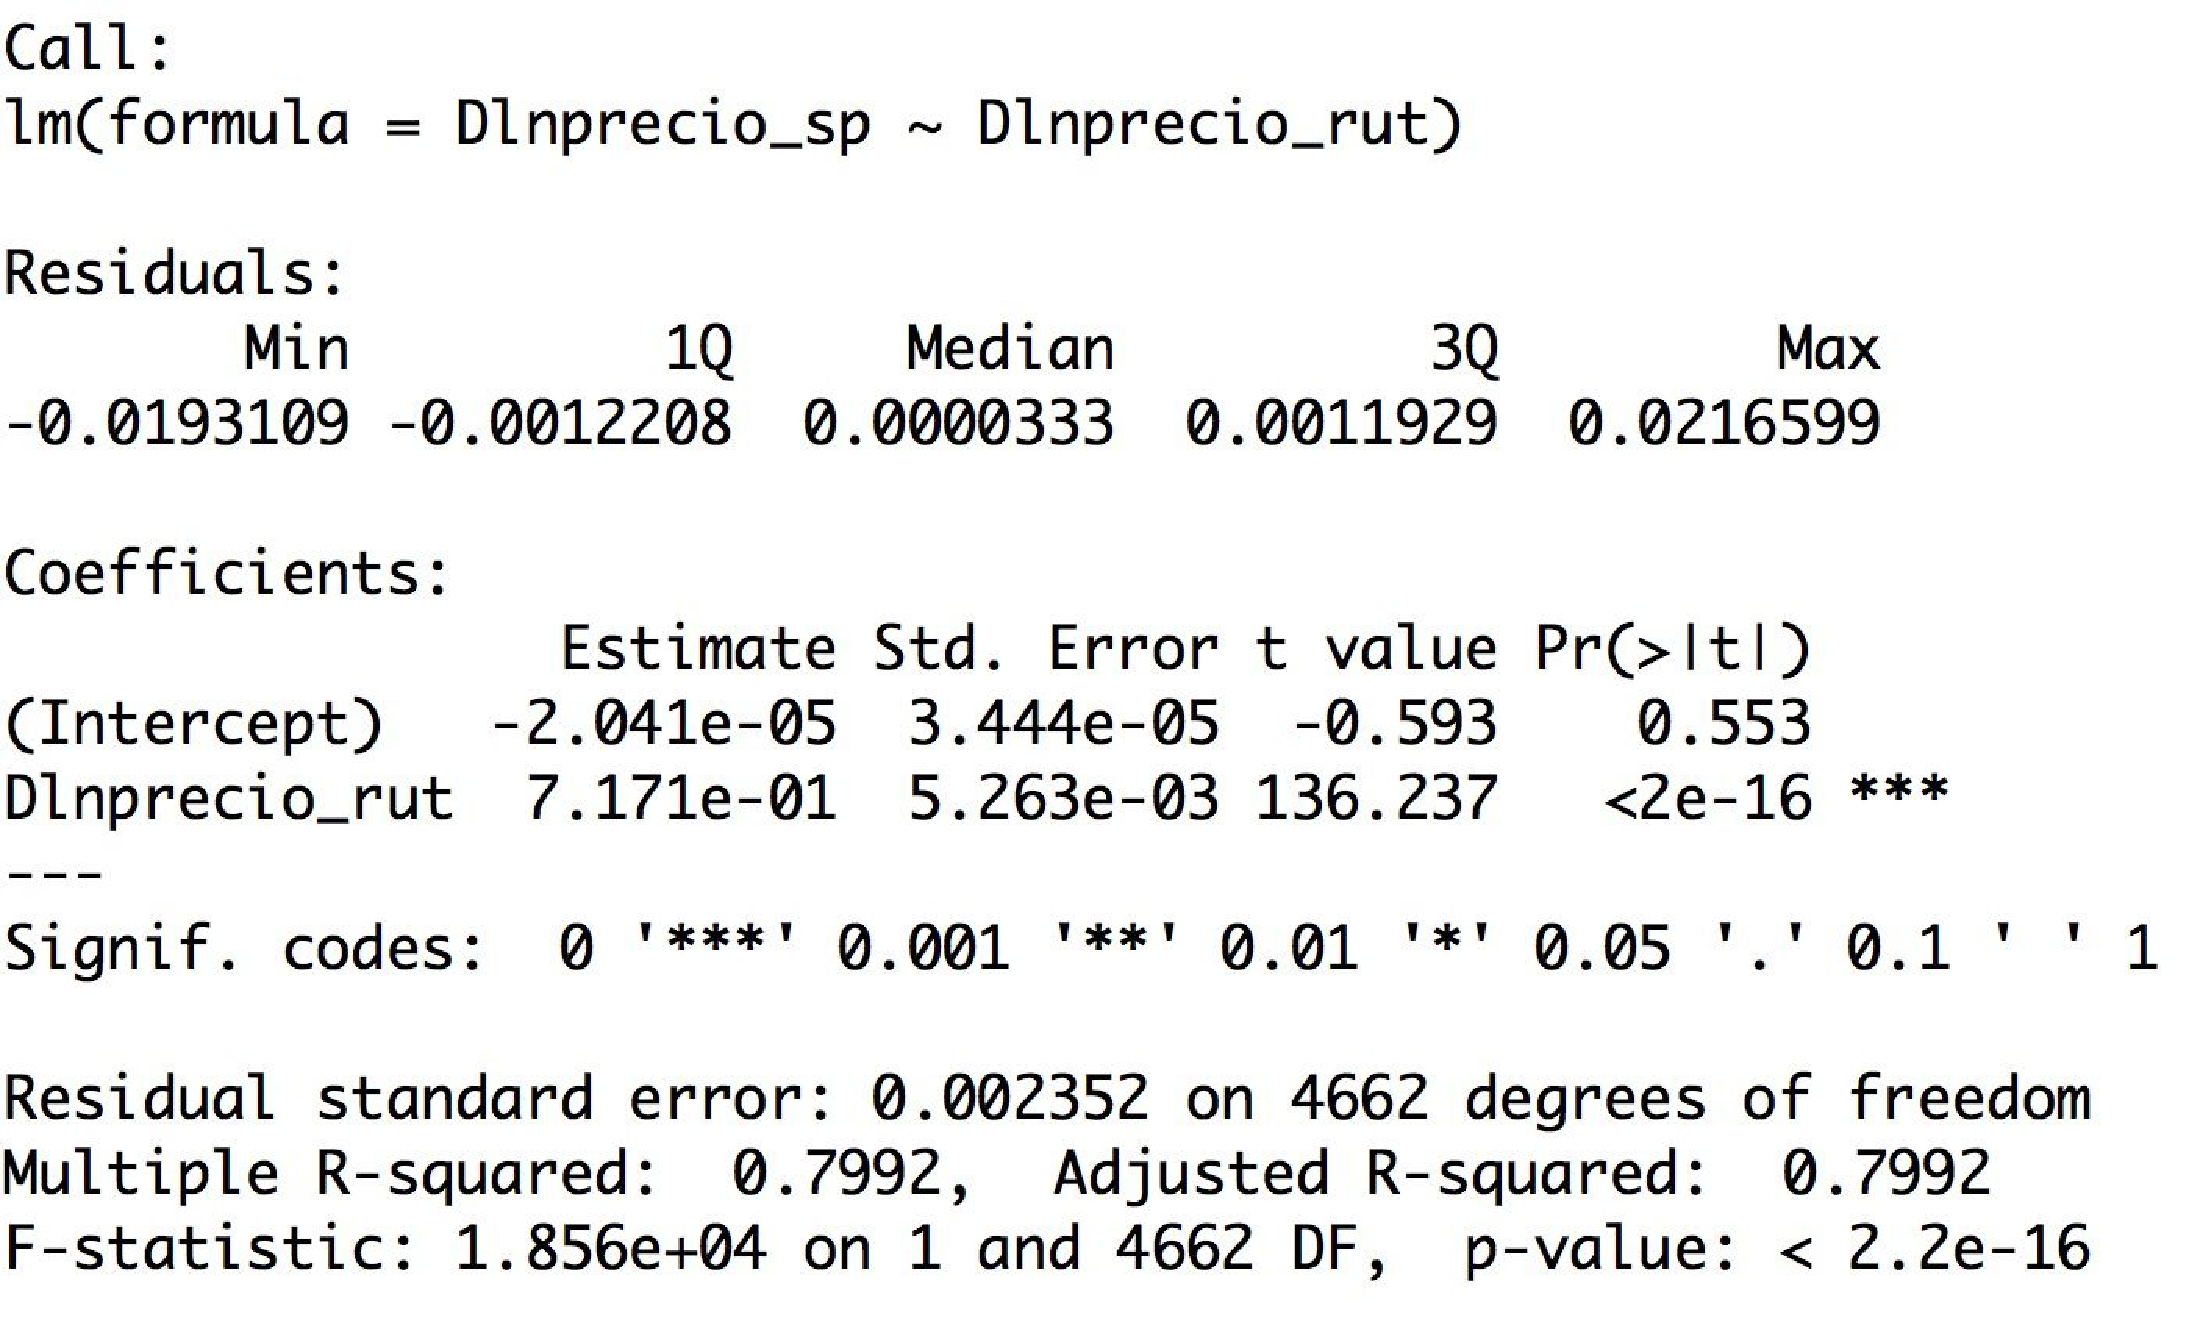
\includegraphics[width=\linewidth]{reg1.pdf}}
%	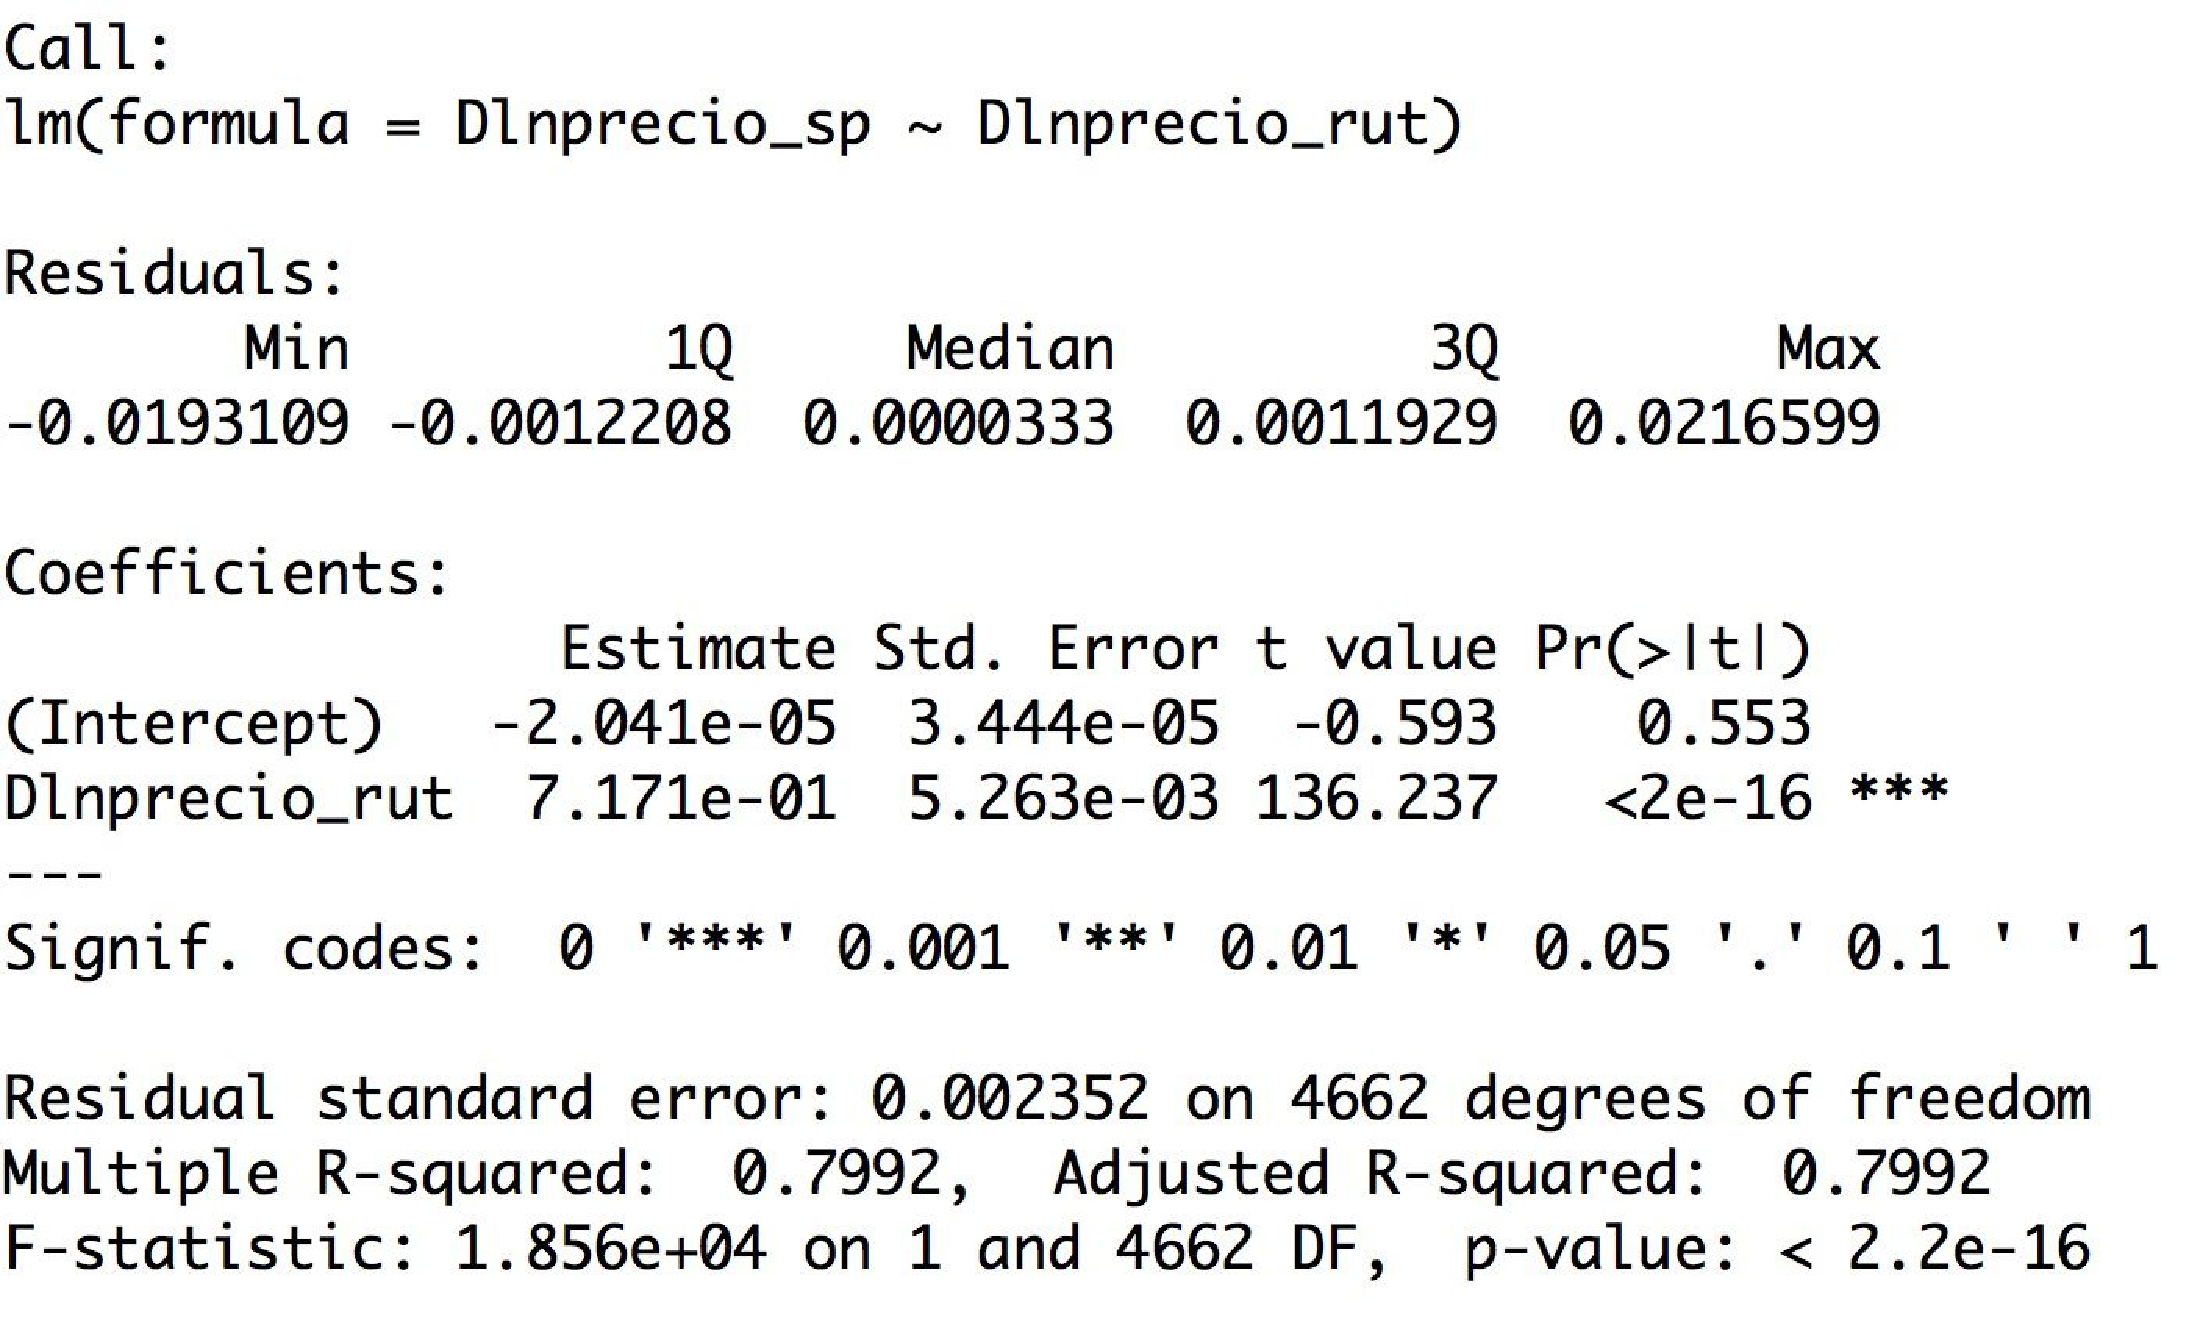
\includegraphics[scale=0.34]{reg1.pdf}
\end{figure}

%\end{frame}
%---------------------------------------------------------

%---------------------Slide 61 --------------------------
%\begin{frame}
%\frametitle{Ejemplo 3: Regresiones}
\lstset{caption = Código R para Regresiones,framexleftmargin=5mm, frame=shadowbox, rulesepcolor=\color{green}}
\begin{lstlisting}[title={‘Código R para Regresiones’},basicstyle=\ttfamily]{}
mydata1 <- read.csv("sp.csv", header=TRUE, 
					stringsAsFactors=FALSE)
precio_sp <- mydata1$"Adj.Close"; 
lnprecio_sp <- log10(precio_sp)
Dlnprecio_sp <- diff(lnprecio_sp ,1)
mydata2 <- read.csv("rut.csv", header= TRUE,
				stringsAsFactors = FALSE)
precio_rut <- mydata2$"Adj.Close" ; 
lnprecio_rut <- log10(precio_rut)
Dlnprecio_rut <- diff(lnprecio_rut ,1)
reg1 <- lm ( Dlnprecio_sp ~ Dlnprecio_rut)
summary(reg1)
\end{lstlisting}\label{ejemplo3Regresiones}
%
%\only<1|handout:1>{
%	\begin{exampleblock}{C\'odigo en R}
%		rm(list=ls())\\
%		mydata $<-$ read.csv (``/Users/marcelovillena/Desktop/sp.csv", header = TRUE, stringsAsFactors = FALSE)\\
%		$precio\_sp$ $<-$ mydata$\$$``Adj.Close" : $lnprecio\_sp$  $<-$ log10($precio\_sp$ ) ; $Dlnprecio\_sp$  $<-$ diff($lnprecio\_sp$ ,1)\\
%		mydata $<-$ read.csv (``/Users/marcelovillena/Desktop/rut.csv", header = TRUE, stringsAsFactors = FALSE)\\
%		$precio\_rut$ $<-$ mydata$\$$``rut" ; lnprecio\_rut  $<-$ log10($precio\_rut$ ) ; $Dlnprecio\_rut$  $<-$ diff($lnprecio\_rut$ ,1)\\
%		reg1 $<-$ lm ( $Dlnprecio\_sp$ $\string ~$ $Dlnprecio\_rut$)\\
%		summary(reg1)
%	\end{exampleblock}
%}
%\end{frame}
%---------------------Slide 62 --------------------------
%\begin{frame}
%\frametitle{Ejemplo 3: Regresioness}

\begin{figure}[H]
	\centering
	\textbf{Russell explicado por SP500}\par\medskip
	\fcolorbox{green}{blue}{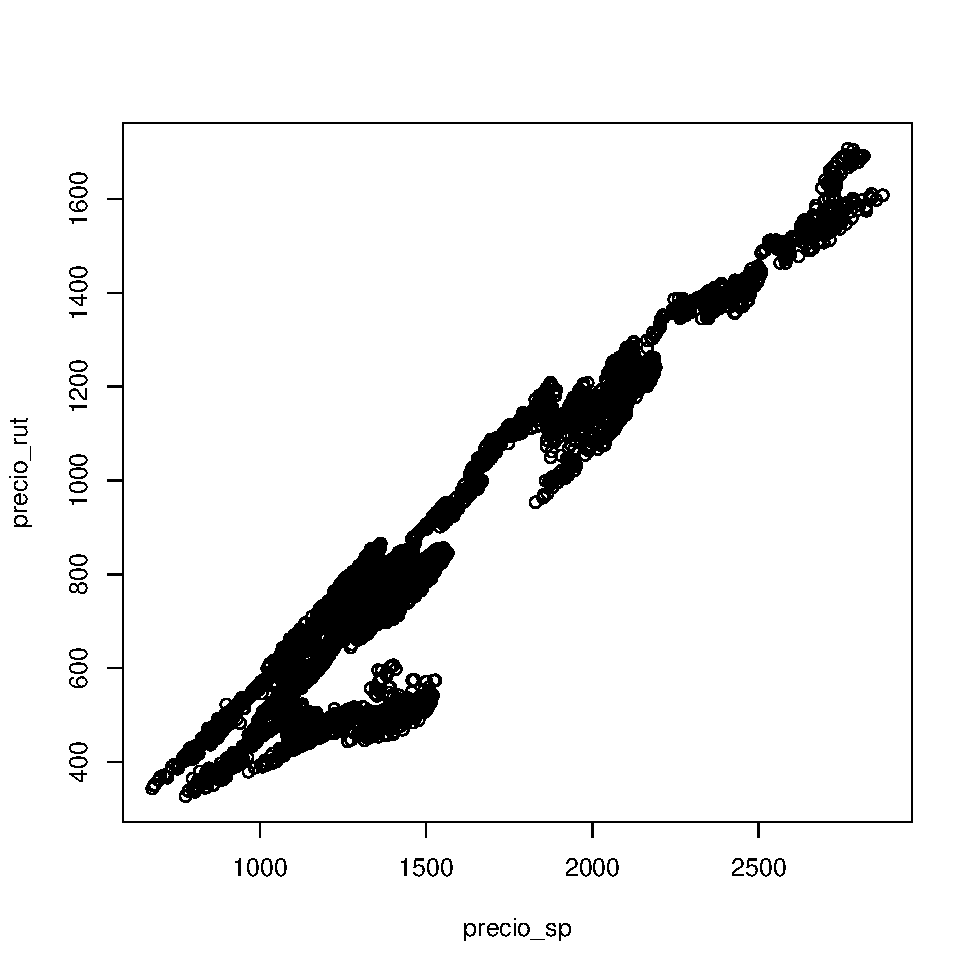
\includegraphics[width=\linewidth]{graph_precios.pdf}}
%	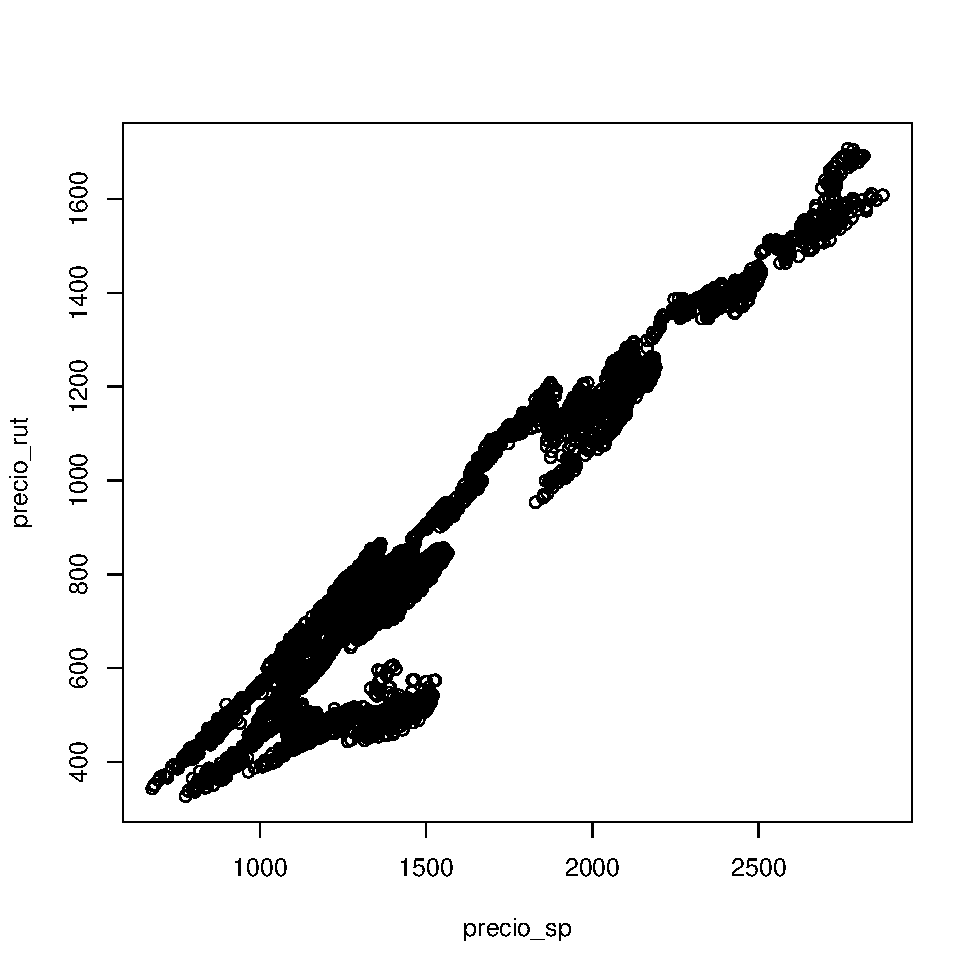
\includegraphics[scale=0.6]{graph_precios.pdf}
	\caption{Regresión de Russell 2000 en función del S\&P500}
\end{figure}

%\end{frame}

%---------------------------------------------------------	
%---------------------Slide 63 --------------------------
%\begin{frame}
%\frametitle{Ejemplo 3: Regresiones}

\pagebreak A partir del siguiente c\'odigo almacenamos los residuos y analizamos los supuestos que exige una buena regresi\'on.
\lstset{caption = Código R para Residuos,framexleftmargin=5mm, frame=shadowbox, rulesepcolor=\color{green}}
\begin{lstlisting}[title={‘Código R para Residuos de regresión’},basicstyle=\ttfamily]{}
residuos <- rstandard(reg1)
valores.ajustados <- fitted(reg1)
plot(valores.ajustados, residuos)
qqnorm(residuos)
qqline(residuos)
\end{lstlisting}\label{ejemplo3ResiduosRegresion}
%\only<1|handout:1>{
%	\begin{exampleblock}{C\'odigo en R}
%		residuos $<-$ rstandard(reg1)\\
%		valores.ajustados $<-$ fitted(reg1)\\
%		plot(valores.ajustados, residuos)\\
%		qqnorm(residuos)\\
%		qqline(residuos)\\
%	\end{exampleblock}
%}
%\end{frame}
%---------------------Slide 54 --------------------------
%\begin{frame}
%\frametitle{Ejemplo 3: Regresiones}



\begin{figure}[H]
	\centering
	\textbf{Homocedasticidad}\par\medskip
	\fcolorbox{green}{blue}{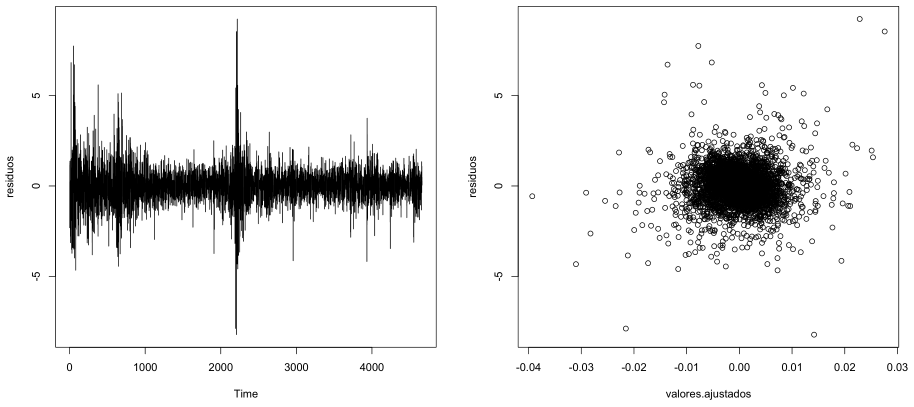
\includegraphics[width=\linewidth]{homocedasticidadD64.png}}
%	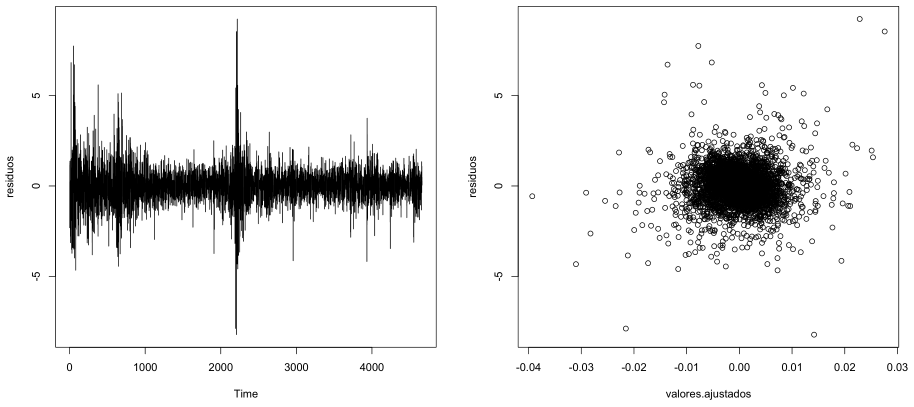
\includegraphics[scale=0.5]{homocedasticidadD64.png}

	\caption[Homocedasticidad]{Izquierda: Derecha}\label{fig11}
\end{figure}

%\end{frame}
%---------------------------------------------------------
%---------------------Slide 65 --------------------------
%\begin{frame}
%\frametitle{Ejemplo 3: Regresiones}



\begin{figure}[H]
	\centering
	\textbf{Normalidad de los residuos}\par\medskip
	\fcolorbox{green}{blue}{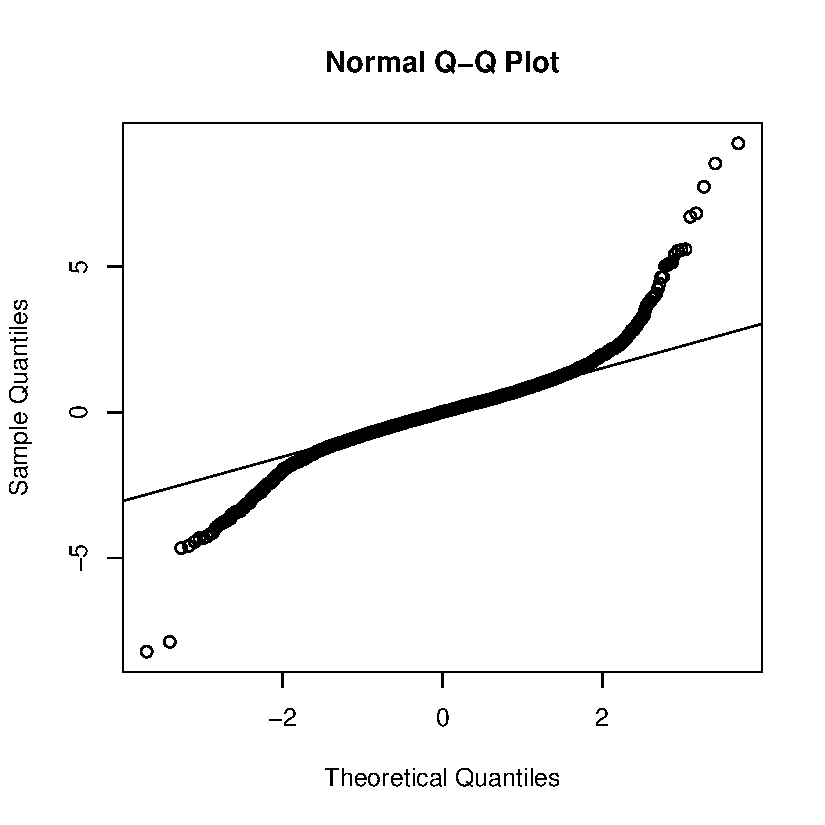
\includegraphics[width=\linewidth]{qqplot_reg1.pdf}}
	\caption{Grafico QQ-Plot de los residuos. La linea punteada indica el comportamiento de una distribución normal, mientras los puntos alejados de ella en los extremos dan cuenta de como se alejan los residuos del comportamiento normal.}
\end{figure}\label{fig12}

%\end{frame}
%\end{section}















%\section{Table}
%
%\begin{table}[htp]
%    \centering
%    \begin{tabular}{r|l|p{10cm}}
%        Right &  Left  &  Longlonglonglonglonglonglonglong longlonglonglonglonglonglonglonglonglonglonglonglong longlonglonglonglonglong \\
%        Right &  Left  &  Longlonglonglonglonglonglong
%        longlonglonglonglonglonglonglong
%        longlonglonglong
%        longlonglonglonglonglonglonglong 
%    \end{tabular}
%    \caption{This is a caption}
%    \label{tab:trans-sym}
%\end{table}
%
%\section{List}
%This is a List:
%\begin{itemize}
%    \item \textbf{Bullet 1}: Bullet 1 is bullet 1.
%    \item \textbf{Bullet 2}: Bullet 2 is bullet 2.
%\end{itemize}
%
%\section{Definition}
%\begin{definition}\label{def:def117}
%\textbf{DEFINITION NAME}: This is a definition.
%\end{definition} 
%
%% avoid bad break
%\vspace{5cm} 
%
%\section{Theorem}
%\begin{theo}[THEOREM NAME]{theo:theo1}
%This is a theorm. Below are equations.
%\begin{align}\label{eq:multi-equations}
%    \psi(\bvec{a}) &= A\cdot \bvec{a} + \bvec{t}.\\
%    R_x &=  \begin{bmatrix} 
%            0 & \cos(\theta) & -\sin(\theta)\\
%            0 & \sin(\theta) & \cos(\theta)\\
%            1 & 0 & 0
%         \end{bmatrix}, 
%    R_y =  \begin{bmatrix} 
%            \cos(\theta) & 0 & -\sin(\theta)\\
%            \sin(\theta) & 0 & \cos(\theta)\\
%            0 & 1 & 0
%         \end{bmatrix}, 
%    R_z =  \begin{bmatrix} 
%            \cos(\theta) & -\sin(\theta) & 0\\
%            \sin(\theta) & \cos(\theta) & 0 \\
%            0 & 0 & 1
%         \end{bmatrix} 
%\end{align}
%\end{theo}
%
%\begin{lem}[LEMMA NAME]{lem:leml}
%This is a lemma
%\end{lem}
%
%\begin{prf}[LEMMA NAME]{prf:leml}
%This is a proof.
%\end{prf}
%
%\section{Tikz Pictures}
%\begin{figure}[htp]
%    \centering
%        \begin{tikzpicture}[scale=0.6]
%            \draw[->] (0,-1)--(0,1.5)node[above] {$s$};
%            \draw[->] (-0.8,0.6) to[bend right] (0.8,0.6);
%            \draw[->] (0.9, 0.8)--(0.9, 1.2) node[right] {$\omega$};
%            \filldraw[dashed] (0,-0.2)--(0.9, -0.3) circle (1pt) node [right] {$q$};
%            \draw[->] (0.8, -0.9)--(1.2, -0.8) node[right] {$v$};
%        \end{tikzpicture}
%    \caption{This is a caption. }
%    \label{fig:rotation}
%\end{figure}

\curinstructor{Marcelo Villena Chamorro PhD.}
\chapter{Tópico II.- Univariate Time Series Models}

\section{Ejemplo de repaso clase anterior-Detrending global temperature}

Como vimos en la clase anterior, la evoluci\'on de la temperatura global manifestaba una tendencia lineal, por lo que podemos asumir que esta puede ser escrita como:
\begin{equation*} 
x_t =\mu_{t} + y_t
\end{equation*}
Veremos dos maneras de descomponer la serie, \textquotedblleft filtrando\textquotedblright \ la tendencia.

%---------------------------------------------------------
%---------------------Slide 4 --------------------------
%\begin{frame}
%\frametitle{Ejemplo de repaso clase anterior\newline
%	Detrending global temperature}

%\only<1|handout:1>{
%	\begin{exampleblock}{C\'odigo en R}
%		rm(list=ls())\\
%		mydata$<-$read.csv (``gtemp.csv")\\
%		gtemp$<-$mydata$\$$``gtem"\\
%		plot(gtemp, type=``o", ylab= ``Global Temperature Deviations'')\\
%		t$<-$1:142\\
%		summary(reg $<-$ lm(gtemp $\string ~$ t))\\
%		plot(gtemp, type=``o", ylab=``Global Temperature Deviations'')\\
%		abline(reg)\\
%	\end{exampleblock}
%}
\lstset{caption=Ejemplo 1 Sacando la tendencia de la serie temperatura global,framexleftmargin=5mm, frame=shadowbox, rulesepcolor=\color{green}}
\begin{lstlisting}[title={‘Código R: ejemplo 1 Obtención de la componente \textquotedblleft tendencia\textquotedblright de la serie temperatura global(gtemp).’},basicstyle=\ttfamily]{}
rm(list=ls())
mydata<-read.csv ("gtemp.csv")
gtemp<-mydata$"gtem"
plot(gtemp, type="o", ylab="Global Temperature Deviations")
t<-1:142
summary(reg <- lm(gtemp ~ t))
plot(gtemp, type="o", ylab="Global Temperature Deviations")
abline(reg)
\end{lstlisting}
%\end{frame}

%---------------------------------------------------------
%---------------------Slide 5--------------------------
%\begin{frame}
%\frametitle{Ejemplo de repaso clase anterior\newline

\begin{figure}[H]
	\centering
	\textbf{Ejemplo 1: Detrending global temperature}\par\medskip
	\fcolorbox{green}{blue}{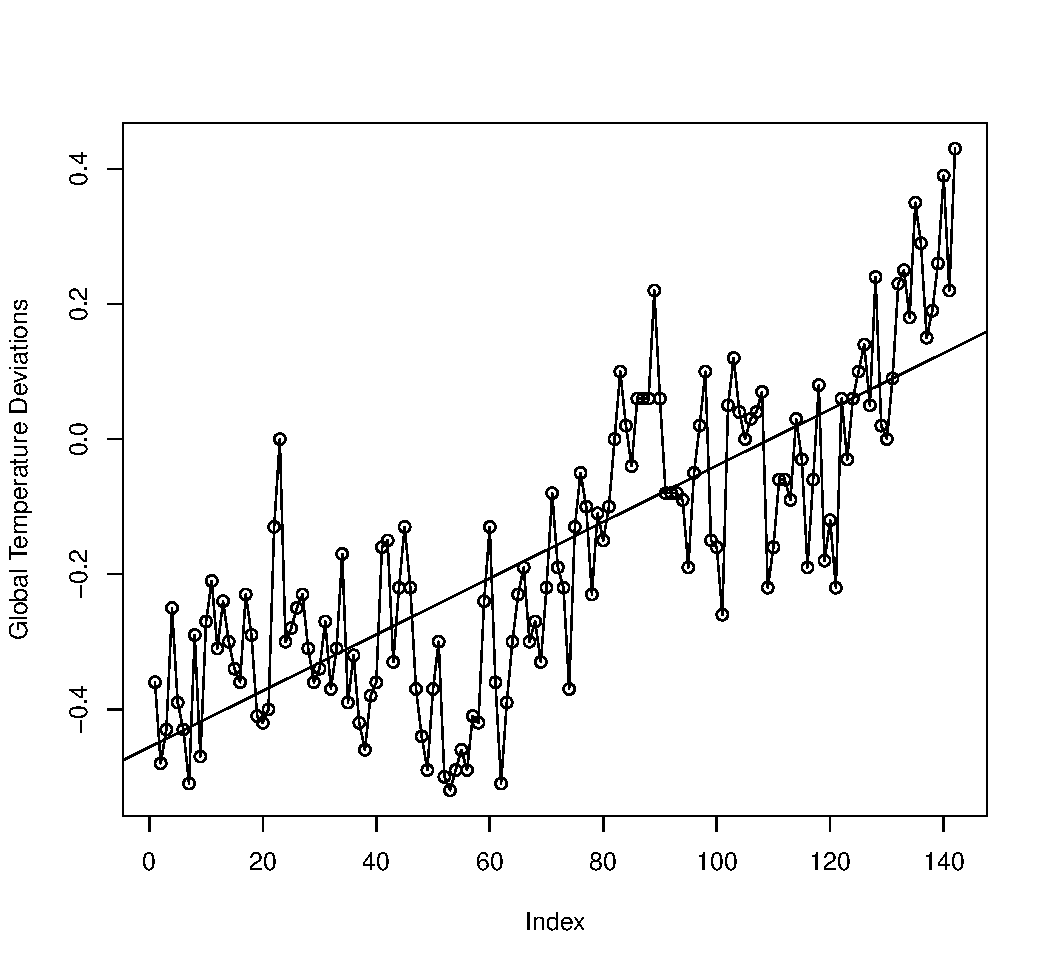
\includegraphics[width=\linewidth,scale=0.5]{gtemp_graph.pdf}}
	\caption{La figura muestra en línea punteada la tendencia de la serie de tiempo.}\label{fig1}
\end{figure}

%\end{frame}
%---------------------------------------------------------
%---------------------Slide 6--------------------------
%\begin{frame}
%\frametitle{Ejemplo de repaso clase anterior\newline
%	Detrending global temperature}

\begin{figure}[H]
	\centering
	\textbf{Detrending global temperature}\par\medskip
	\fcolorbox{green}{blue}{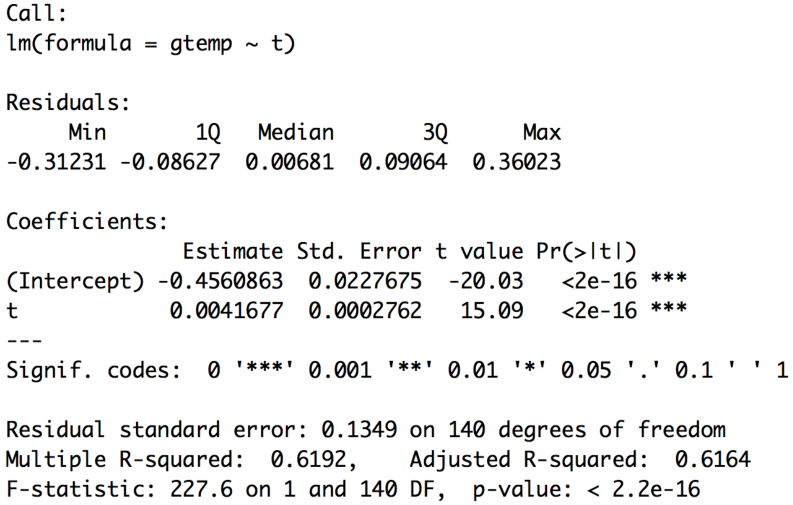
\includegraphics[width=\linewidth,scale=0.5]{reg_ej1.png}}
	\caption{Parametría de la regresión de temperatura en el tiempo.}\label{fig2}
\end{figure}

%\end{frame}
%---------------------------------------------------------
%---------------------Slide 7 --------------------------
%\begin{frame}
%\frametitle{Ejemplo de repaso clase anterior\newline
%	Detrending global temperature}

%\only<1|handout:1>{
%	\begin{exampleblock}{C\'odigo en R}
%		reg1= lm(gtemp$\string ~$ time(gtemp), na.action=NULL) \\
%		par(mfrow=c(2,1))\\
%		plot(resid(reg1), type=``o", main=``detrended")\\
%		plot(diff(gtemp), type=``o", main=``first difference")\\
%	\end{exampleblock}
%}
\lstset{caption=Ejemplo 1 Detrending global temperature,framexleftmargin=5mm, frame=shadowbox, rulesepcolor=\color{green}}
\begin{lstlisting}[title={‘Código R: ejemplo 1 Regresando gtemp sobre tiempo.’},basicstyle=\ttfamily]{}
reg1= lm(gtemp~time(gtemp), na.action=NULL) 
par(mfrow=c(2,1))
plot(resid(reg1), type="o", main="detrended")
plot(diff(gtemp), type="o", main="first difference")
\end{lstlisting}
%\end{frame}
%=================================
%---------------------Slide 8--------------------------
%\begin{frame}
%\frametitle{Ejemplo de repaso clase anterior\newline
%	Detrending global temperature}

\begin{figure}[H]
	\centering
	\textbf{Ejemplo 1: Detrending global temperature}\par\medskip
	\fcolorbox{green}{blue}{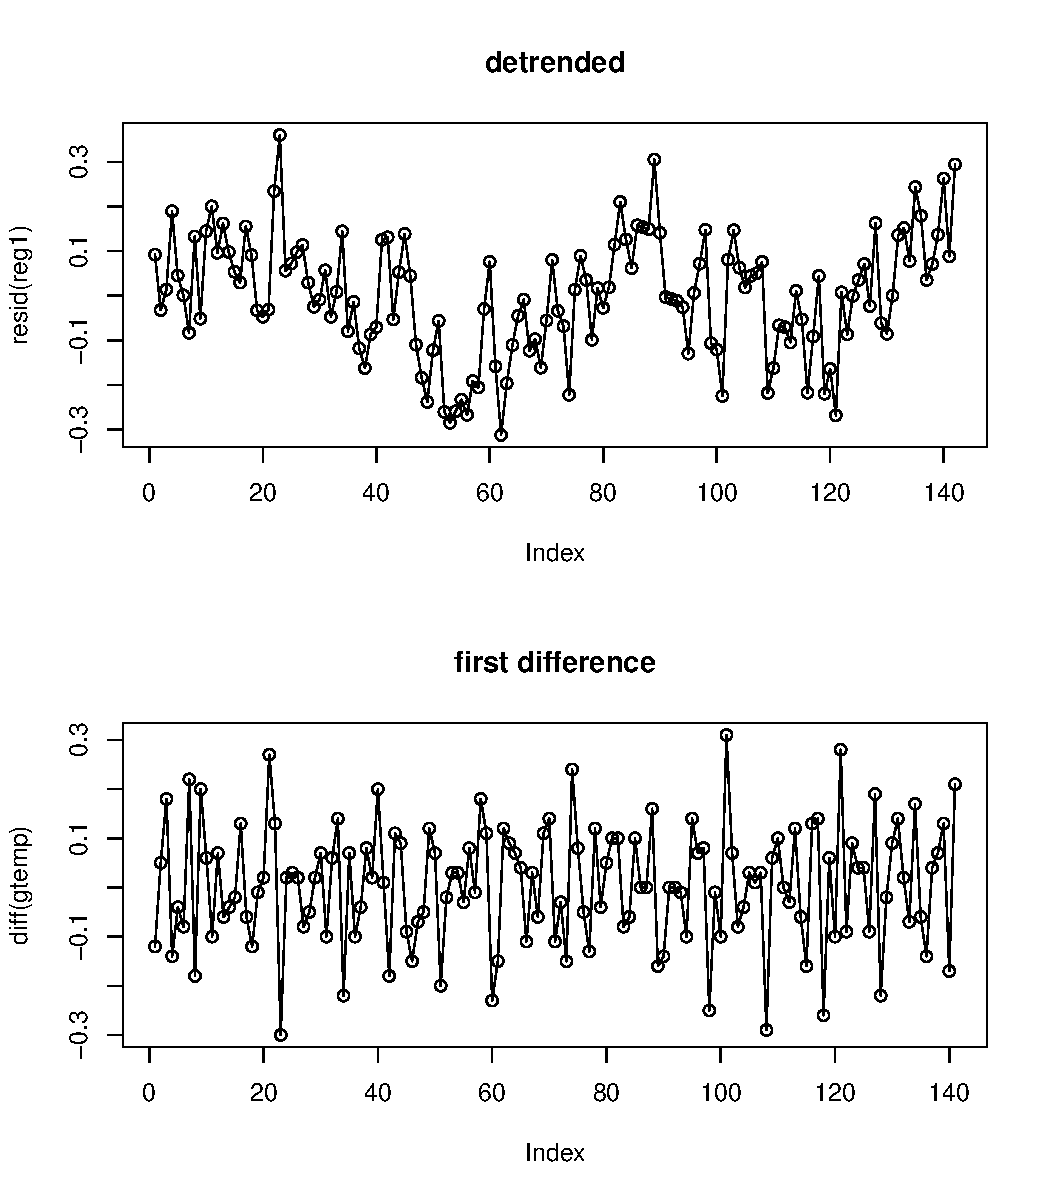
\includegraphics[width=\linewidth,scale=0.5]{detrended.pdf}}
	\caption{Arriba: residuos de la regresión. Abajo:primeras diferencias de la serie original}\label{fig3}
\end{figure}

%\begin{figure}[p]
%	\centering
%	\textbf{Detrending global temperature}\par\medskip
%	\fcolorbox{red}{yellow}{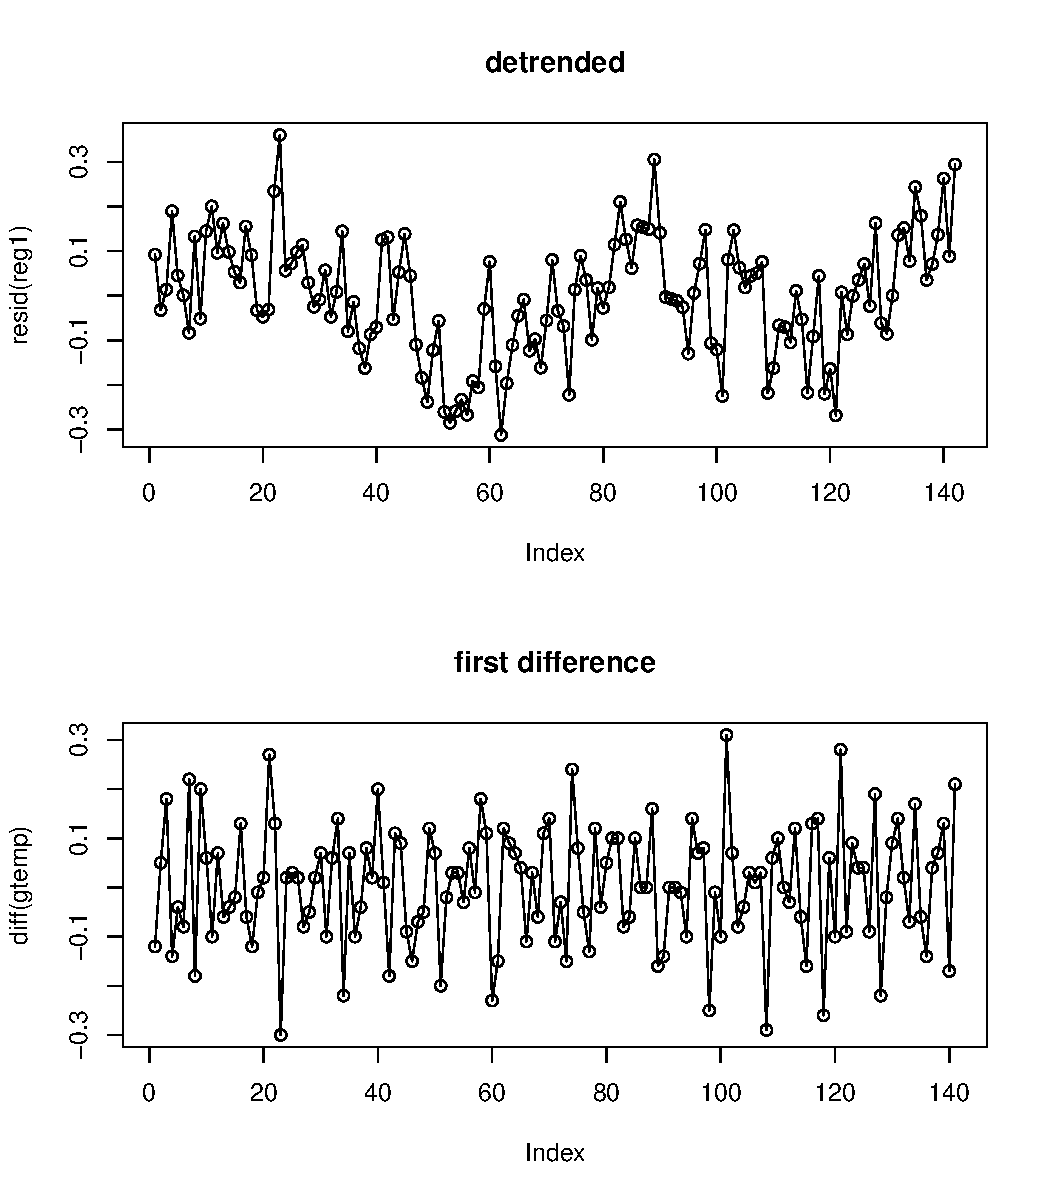
\includegraphics[width=\linewidth,scale=0.5]{detrended.pdf}}
%	\caption{Arriba: residuos de la regresión. Abajo:primeras diferencias de la serie original}\label{fig3.2}
%\end{figure}

%\end{frame}

%---------------------------------------------------------
%---------------------Slide 9 --------------------------
%\begin{frame}
%\frametitle{Ejemplo de repaso clase anterior\newline
%Detrending global temperature}

%\only<1|handout:1>{
%\begin{exampleblock}{C\'odigo en R}
%	par(mfrow=c(3,1)) \\
%	acf(gtemp, 48, main=``gtemp")\\
%	acf(resid(reg), 48, main=``detrended")\\
%	acf(diff(gtemp), 48, main=``first difference")\\
%\end{exampleblock}
%}
\lstset{caption=Ejemplo 1 Detrending global temperature,framexleftmargin=5mm, frame=shadowbox, rulesepcolor=\color{green}}
\begin{lstlisting}[title={‘Código R: ejemplo 1 Correlogramas de series.’},basicstyle=\ttfamily]{}
par(mfrow=c(3,1)) # plot ACFs
acf(gtemp, 48, main="gtemp")
acf(resid(reg), 48, main="detrended")
acf(diff(gtemp), 48, main="first difference")
\end{lstlisting}

%\end{frame}
%---------------------------------------------------------
%---------------------Slide 10--------------------------
%\begin{frame}
%\frametitle{Ejemplo de repaso clase anterior\newline
%Detrending global temperature}

\begin{figure}[H]
	\centering
	\textbf{Ejemplo 1: Autocorrelograma}\par\medskip
	\fcolorbox{green}{blue}{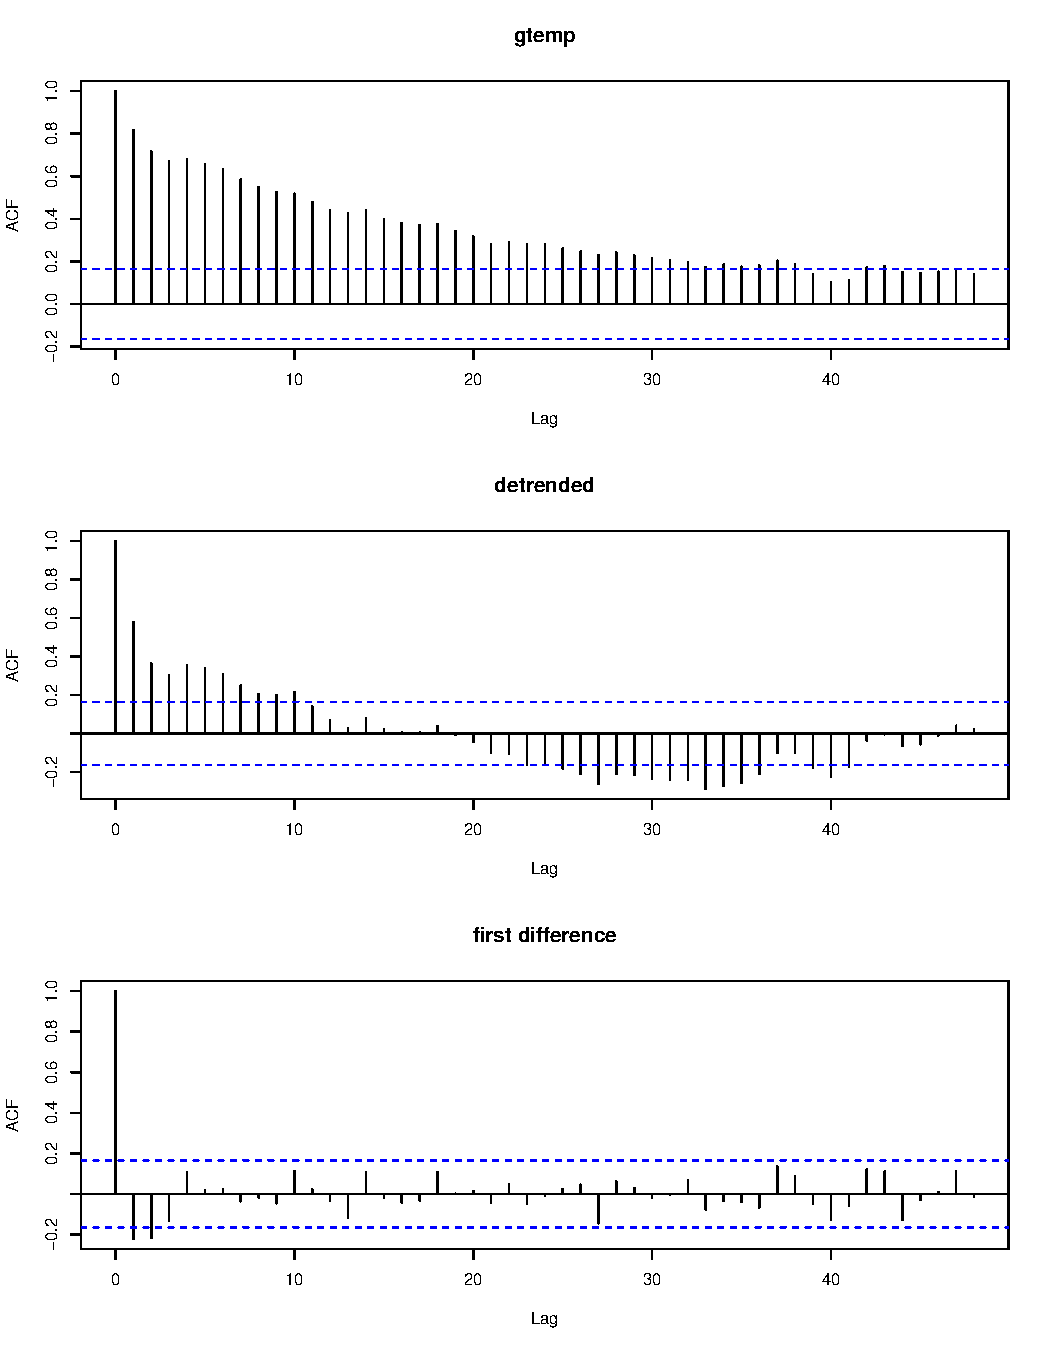
\includegraphics[width=\linewidth,scale=0.5]{acf_example1.pdf}}
	\caption{Autocorrelogramas para diferentes retardos(lags): Arriba:serie original. Medio: residuos de la regresión. Abajo: primera diferencia de la serie original}\label{fig4}
\end{figure}

%\end{frame}
%---------------------------------------------------------
%---------------------Slide 11--------------------------
%\begin{frame}
%\frametitle{Sobre la descomposici\'on de una serie}
\pagebreak\section{Sobre la descomposici\'on de una serie}

En los gr\'aficos podemos apreciar que la primera diferencia de la serie produce resultados diferentes a la eliminaci\'on de la tendencia mediante la regresi\'on de la tendencia.\\
En el caso de los gr\'aficos ACF, el proceso diferenciado muestra una autocorrelaci\'on mi\'{\i}nima, lo que puede implicar que la serie de temperatura global es similar una caminata aleatoria con deriva.\\
Es interesante notar que si la serie es una caminata aleatoria con deriva, la media de la serie diferenciada, que es una estimaci\'on de la deriva, es aproximadamente $,0066$, pero con un gran error est\'andar:\\
%\only<1|handout:1>{
%	\begin{exampleblock}{C\'odigo en R}
%		mean (diff (gtemp))\\
%		sd (diff (gtemp)) / sqrt (longitud (diff (gtemp)))
%	\end{exampleblock}
%}
\lstset{caption=Ejemplo 1 Detrending global temperature,framexleftmargin=5mm, frame=shadowbox, rulesepcolor=\color{green}}
\begin{lstlisting}[title={‘Código R: ejemplo 1: sobre la descomposición de una serie - media y error estandar’},basicstyle=\ttfamily]{}
mean (diff(gtemp)) #media
sd (diff (gtemp)) / sqrt (length(diff (gtemp))) #error estandar
\end{lstlisting}
%\end{frame}
%---------------------------------------------------------
%---------------------Slide 12--------------------------

%\begin{frame}
%\frametitle{Sobre la descomposici\'on de una serie}

Una ventaja de diferenciar sobre la estimaci\'on de una tendencia,  para eliminar las tendencias, es que no se estiman par\'ametros en la operaci\'on de diferenciaci\'on. Una desventaja, sin embargo, es que la diferenciaci\'on no arroja una estimaci\'on del proceso estacionario $y_t$.\\
%\vspace{5mm}	 
De esta forma, si una estimaci\'on de $y_t$ es esencial, entonces la estimación de una tendencia puede ser la forma más apropiada para eliminar las tendencias de la serie. Si el objetivo es forzar los datos a la estacionaridad, entonces la diferenciaci\'on puede ser m\'as apropiada. La diferenciaci\'on tambi\'en es una herramienta viable si la tendencia es fija.\\
%\vspace{3mm}	
En EE.UU. el procedimiento oficial de descomposici\'on y ajuste estacional se llama:\\
%\vspace{3mm}	
\textbf{X-13-ARIMA (http://www.census.gov/srd/www/x13as/)}

%\end{frame}

%---------------------------------------------------------
%---------------------Slide 13--------------------------

%\begin{section}{Procesos no estacionarios, integrados y el test de ra\'{\i}z unitaria}
\pagebreak\section{Procesos no estacionarios, integrados y el test de ra\'{\i}z unitaria}
%\begin{frame}
%\frametitle{Procesos no estacionarios, integrados y el test de ra\'{\i}z unitaria}

Recordemos que si una serie de tiempo es estacionaria, su media, su varianza y su autocovarianza (en diferentes rezagos) permanecen iguales sin importar el momento del tiempo en el cual se midan; es decir, son \textbf{invariantes respecto al tiempo}.
\par
Por otro lado, hemos visto que la estacionaridad es una caracter\'{\i}stica deseable, por ejemplo, en t\'erminos de la normalidad de las variables. Sin embargo, en la pr\'actica nos encontramos con:
\par
%\only<1->{
\begin{itemize}
	\item[(i)] Procesos No-estacionarios: Cuando un proceso estoc\'astico de series de tiempo es dependiente del tiempo.
	\item[(ii)] Procesos Integrados: un proceso no-estacionario, el cual puede ser transformado a proceso estacionario diferenciando.
\end{itemize}
%}

%\end{frame}

%---------------------------------------------------------
%---------------------Slide 14--------------------------
%\begin{frame}
%\frametitle{Procesos Integrados}
\subsection{Procesos Integrados}

Con respecto a los Procesos Integrados, partimos definiendo:
%\only<1->{
	\begin{itemize}
		\item La secuencia $\{x_t\}$ es integrada de orden $d$, $I(d)$, si esta requiere ser diferenciada $d$ veces para llegar a ser estacionaria.
		\item Todos los \textbf{Procesos Integrados son no-estacionarios}, pero no todos los procesos no-estacionarios son integrados.
		\item Si la secuencia $\{x_t\}$  tiene una ra\'{\i}z unitaria, entonces, es un proceso integrado, y de aqu\'{\i} no-estacionario.
	\end{itemize}
%}
%
%\end{frame}

%---------------------------------------------------------
%---------------------Slide 15--------------------------
%\begin{frame}
%\frametitle{Consecuencias de los Procesos Integrados (Ra\'{\i}z Unitaria)}
\subsection{Consecuencias de los Procesos Integrados (Ra\'{\i}z Unitaria)}
%\only<1->{
\begin{itemize}
	\item Es importante se\~nalar que los test estad\'{\i}sticos est\'andares no son apropiados cuando los MCO (OLS) son aplicados a procesos integrados, ver por ejemplo \cite{granger1974spurious}.
	\item Si la secuencia $\{x_t\}$ es un proceso de ra\'{\i}z unitaria, entonces, cualquier shock tiene un efecto permanente (que no decae). De aqu\'{\i}, la serie de tiempo es modelada apropiadamente suponiendo una tendencia estoc\'astica. La serie de tiempo entonces puede ser definida como estacionaria diferenciable, y se le deber\'a sacar la tendencia diferenciando. 
	\item En este contexto, \textbf{los t\'erminos no-estacionariedad, caminata aleatoria, ra\'{\i}z unitaria y tendencia estoc\'astica se consideran sin\'onimos}. 
\end{itemize}
%}
%
%\end{frame}

%---------------------------------------------------------
%---------------------Slide 16--------------------------
%\begin{frame}
%\frametitle{Test de Ra\'{\i}z Unitaria}
\subsection{Test de Ra\'{\i}z Unitaria}
Considere el siguiente proceso autoregresivo:

\begin{equation} \label{AR1}
x_t =\alpha_1 x_{t-1} + \epsilon_t
\end{equation}

Si $\alpha_1=1$, la secuencia $x_t$ es una ra\'{\i}z unitaria.

El test est\'andar para probar esta hip\'otesis, consiste en restar $x_{t-1}$ a la ecuaci\'on anterior de forma que:

\begin{equation}
\triangle x_t =\gamma x_{t-1} + \epsilon_t
\end{equation}

donde $\gamma=\alpha_1-1$, y $\triangle x_t = x_t - x_{t-1}$. En este contexto, probar la hip\'otesis que la ecuaci\'on (1) tiene una ra\'{\i}z unitaria, $\alpha_1 = 1$, es equivalente a probar la hip\'otesis de $\gamma=0$ en ecuaci\'on (2). 
Este es b\'asicamente el enfoque de Dickey-Fuller (DF) para ra\'{\i}ces unitarias, ver por ejemplo \cite{dickey1981likelihood}. Adicionalmente existe el test aumentado de Dickey-Fuller (ADF), y muchos otros tests que se basan el l\'ogicas similares, y que utilizaremos durante el curso.

%\end{frame}

%---------------------------------------------------------
%---------------------Slide 17 --------------------------
%\begin{frame}
%\frametitle{Ejemplo de Test de Ra\'{\i}z Unitaria - Dickey-Fuller}
\subsubsection{Ejemplo de Test de Ra\'{\i}z Unitaria - Dickey-Fuller}
%\only<1|handout:1>{
%\begin{exampleblock}{C\'odigo en R}
%install.packages(``tseries")\\
%library(tseries)\\
%adf.test(gtemp)\\
%adf.test(resid(reg1))\\
%adf.test(diff(gtemp))\\
%\end{exampleblock}
%}
\lstset{caption=Ejemplo ,framexleftmargin=5mm, frame=shadowbox, rulesepcolor=\color{green}}
\begin{lstlisting}[title={‘Código R: Ejemplo Test de Raíz Unitaria - Dickey-Fuller ’},basicstyle=\ttfamily]{}
library(tseries)
adf.test(gtemp)
adf.test(resid(reg1))
adf.test(diff(gtemp))
\end{lstlisting}
%\end{frame}
%---------------------------------------------------------
%---------------------Slide 18 --------------------------
%\begin{frame}
%\frametitle{Ejemplo de Test de Ra\'{\i}z Unitaria - Dickey-Fuller}
%\begin{mdframed}[style=MyFrame]
%Augmented Dickey-Fuller Test\\
%data:  gtemp\\
%Dickey-Fuller = -2.0624, Lag order = 5, p-value =
%0.5505\\
%alternative hypothesis: stationary\\
%\vspace{5mm}	    
%Augmented Dickey-Fuller Test\\
%data:  resid(reg1)\\
%Dickey-Fuller = -2.0624, Lag order = 5, p-value =
%0.5505\\
%alternative hypothesis: stationary\\
%\vspace{5mm}	    
%Augmented Dickey-Fuller Test\\
%data:  diff(gtemp)\\
%Dickey-Fuller = -6.8179, Lag order = 5, p-value = 0.01\\
%alternative hypothesis: stationary\\
%\end{mdframed}

\begin{figure}[H]
	\centering
	\textbf{Ejemplo: Resultados de Test de Raíz Unitaria - Dickey-Fuller}\par\medskip
	\fcolorbox{green}{blue}{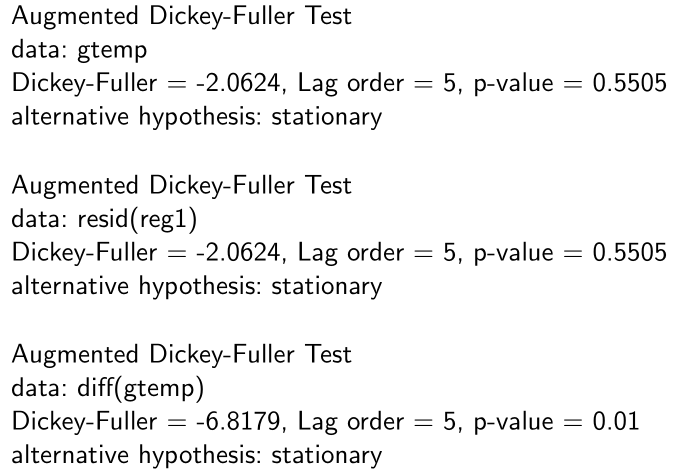
\includegraphics[width=\linewidth,scale=0.5]{adf_ejRaizUnitaria.png}}
	\caption{Test de raíz unitaria Dickey-Füller para diferentes series: Arriba:serie original (gtemp). Medio: residuos de la regresión(resid(reg1)). Abajo: primera diferencia de la serie original (diff(gtemp))}\label{fig5}
\end{figure}
%\end{frame}
%
%\end{section}
%---------------------------------------------------------
%---------------------Slide 19--------------------------
%\begin{section}{Modelos ARIMA: modelando el corto plazo}
%\begin{frame}
%\frametitle{Modelos ARIMA: modelando el corto plazo}
\pagebreak\section{Modelos ARIMA: modelando el corto plazo}

En el a\~no 1970, la metodolog\'{\i}a propuesta por George Box y Gwilym Jenkins, \cite{BoxJenkins} , dos ingenieros con formaci\'on estad\'{\i}stica sistematizan modelos estad\'{\i}sticos para el an\'alisis de series temporales univariantes, teniendo en cuenta para esto la dependencia existente entre los datos. \\
As\'{\i}, cada observaci\'on es modelada en funci\'on de los valores anteriores, la variable tiempo, por tanto, juega un papel fundamental. 

%\end{frame}

%---------------------------------------------------------
%---------------------Slide 20--------------------------
%\begin{frame}
%\frametitle{Modelos ARIMA: modelando el corto plazo}


Los modelos de predicci\'on de Box-Jenkins pertenecen a la familia de modelos alg\'ebraicos lineales, que consideran que una serie temporal real constituye una probable realizaci\'on de un determinado proceso estoc\'astico.\\
\vspace{4mm}	
Estos modelos se conocen con el nombre gen\'erico de ARIMA (Auto-regresive Integrated Moving Average), el cual deriva de sus tres componentes Autoregresivo (AR), Integrado (I) de Medias M\'oviles (MA). Modelar una serie temporal supone identificar un modelo ARIMA adecuado que se ajuste a la serie objeto de estudio, debe contener los m\'{\i}nimos elementos necesarios para describir el fen\'omeno y ser \'util para realizar previsiones.

%\end{frame}
%---------------------------------------------------------
%---------------------Slide 21--------------------------
%\begin{frame}
%\frametitle{Sobre el operador de retroceso - backshift operator}
\subsection{Sobre el operador de retroceso - backshift operator}
\begin{mdframed}[style=MyFrame]
\begin{definition}\label{def}
	\textbf{Definici\'on: operador de retroceso (backshift operator):}
		\begin{equation}
		B x_t = x_{t-1} 
		\end{equation}
		\begin{equation}
		B^2 x_t =  B(B x_t) = B x_{t-1} = x_{t-2}
		\end{equation}
		As\'{\i}:
		\begin{equation}
		B^k x_t = x_{t-k} 
		\end{equation} 
\end{definition}
\end{mdframed}

%\only<1|handout:1>{
%	\begin{block}{Definici\'on: operador de retroceso (backshift operator) }
%		Definimos el operador de retroceso (backshift operator) como:
%		
%		\begin{equation}
%		B x_t = x_{t-1} 
%		\end{equation}
%		\begin{equation}
%		B^2 x_t =  B(B x_t) = B x_{t-1} = x_{t-2}
%		\end{equation}
%		As\'{\i}:
%		\begin{equation}
%		B^k x_t = x_{t-k} 
%		\end{equation}
%	\end{block}
%}

De esta forma tenemos que la primera diferencia se puede definir en t\'erminos de lags, en otras palabras del operador de retroceso:
\begin{equation}
\triangle x_t = x_t - x_{t-1}= (1 - B) x_t 
\end{equation}
En general:
\begin{equation}
\triangle^d x_t = (1 - B)^d x_t 
\end{equation}

%\end{frame}
%---------------------------------------------------------
%---------------------Slide 22--------------------------
%\begin{frame}
%\frametitle{Modelos ARIMA: modelando el corto plazo}
\begin{mdframed}[style=MyFrame]
\begin{definition}\label{def2}
	\textbf{Definici\'on:  $AR (p)$:}
	Un modelo autorregresivo de orden p, frecuentemente abreviado como $AR(p)$, tiene la forma:
	\begin{equation}
	x_t = \phi_1 x_{t-1} +  \phi_2 x_{t-2} + \dots{} +  \phi_p x_{t-p} + \epsilon_t
	\label{ar}
	\end{equation}
	donde $x_t$ es una serie estacionaria, y  $\phi_1$,  $\phi_2$,  \dots{} , $\phi_p$ son constantes. 
	Si la media de $x_t$ es $\mu$, entonces podemos reemplazar $x_t-\mu$ en $\eqref{ar}$
	\begin{equation}
	x_t-\mu = \phi_1 (x_{t-1}-\mu) +  \phi_2 (x_{t-2}-\mu) + \dots{} +  \phi_p (x_{t-p}-\mu) + \epsilon_t
	\end{equation}
	\begin{equation}
	x_t = \alpha + \phi_1 x_{t-1} +  \phi_2 x_{t-2} + \dots{} +  \phi_p x_{t-p} + \epsilon_t
	\end{equation}
	donde $\alpha = \mu(1-\phi_1-\phi_2\dots{}\phi_p)$\\
	Usando los operadores de retroceso $AR(p)$ queda como:
	\begin{equation}
	(1- \phi_1 B + \phi_2 B^2 - \dots{}  - \phi_p B^p )
	\end{equation}
	o incluso m\'as concisamente
	\begin{equation}
	\phi (B) x_t = \epsilon_t
	\end{equation}	
\end{definition}
\end{mdframed}

%\only<1|handout:1>{
%\begin{block}{Definici\'on: $AR (p)$}
%	Un modelo autorregresivo de orden p, frecuentemente abreviado como $AR(p)$, tiene la forma:
%	\begin{equation}
%	x_t = \phi_1 x_{t-1} +  \phi_2 x_{t-2} + \dots{} +  \phi_p x_{t-p} + \epsilon_t
%	\label{ar}
%	\end{equation}
%	donde $x_t$ es una serie estacionaria, y  $\phi_1$,  $\phi_2$,  \dots{} , $\phi_p$ son constantes. 
%	Si la media de $x_t$ es $\mu$, entonces podemos reemplazar $x_t-\mu$ en $\eqref{ar}$
%	\begin{equation}
%	x_t-\mu = \phi_1 (x_{t-1}-\mu) +  \phi_2 (x_{t-2}-\mu) + \dots{} +  \phi_p (x_{t-p}-\mu) + \epsilon_t
%	\end{equation}
%	\begin{equation}
%	x_t = \alpha + \phi_1 x_{t-1} +  \phi_2 x_{t-2} + \dots{} +  \phi_p x_{t-p} + \epsilon_t
%	\end{equation}
%	donde $\alpha = \mu(1-\phi_1-\phi_2\dots{}\phi_p)$\\
%	Usando los operadores de retroceso $AR(p)$ queda como:
%	\begin{equation}
%	(1- \phi_1 B + \phi_2 B^2 - \dots{}  - \phi_p B^p )
%	\end{equation}
%	o incluso m\'as concisamente
%	\begin{equation}
%	\phi (B) x_t = \epsilon_t
%	\end{equation}
%\end{block}
%}

%\end{frame}

%---------------------------------------------------------
%---------------------Slide 23--------------------------
%\begin{frame}
%\frametitle{Ejemplo Proceso Autoregresivo de Orden 1: AR(1)}
\subsection{Ejemplo Proceso Autoregresivo de Orden 1: AR(1)}

En un procesos AR(1) la variable $x_t$ queda \'unicamente por su valor pasado $x_{t-1}$:
\begin{equation}
x_t = \phi x_{t-1} + \epsilon_t
\end{equation}

donde como sabemos $\epsilon_t$ es un proceso de ruido blanco con media cero y varianza constante $\sigma^2$, y $\phi$ es un par\'ametro. Para verificar que el modelo AR(1) es estacionario debemos probar que es:\\
\vspace{4mm}	
\textbf{(1) Estacionario en media}
\begin{equation}
E(x_t) = E(\phi x_{t-1} + \epsilon_t)=\phi E(x_{t-1} )
\end{equation}
Para que el proceso sea estacionario, la media debe ser constante y finita en el tiempo, lo que implica:
\begin{equation}
E(x_t) = \phi E(x_{t} )
E(x_t) = \frac{0}{1-\phi}=0
\end{equation}
\\
Por lo tanto, para que el proceso sea estacionario el par\'ametro $\phi \ne 0$.

%\end{frame}

%---------------------------------------------------------
%---------------------Slide 24--------------------------
%\begin{frame}
%\frametitle{Ejemplo Proceso Autoregresivo de Orden 1: AR(1)}

\textbf{(2) Estacionario en covarianza}

Para verificar que el modelo AR(1) sea estacionario, la varianza debe ser constante y finita en el tiempo:

\begin{equation}
\gamma = E(x_t-E(x_t))^2 = E(\phi x_{t-1} + \epsilon_t - 0)^2 = \phi^2 var(x_{t-1}) + \sigma^2
\end{equation}

Asumiendo que el proceso es estacionario:
\begin{equation}
E(x_t)^2 = var(x_{t-1}) = var(x_{t}) = \gamma
\end{equation}
De aqu\'{\i} tenemos que:

\begin{equation}
\gamma  = \phi^2 \gamma + \sigma^2
\end{equation}

Por lo que:
\begin{equation}
\gamma  = \frac{\sigma^2}{1-\phi^2}
\end{equation}\\
Para que un proceso sea estacionario, varianza constante y finita, es necesario que $|\phi|< 1$.
%\end{frame}

%---------------------------------------------------------
%---------------------Slide 25--------------------------
%\begin{frame}
%\frametitle{Ejemplo Proceso Autoregresivo de Orden 1: AR(1)}

Si se cumple que $|\phi|< 1$, entonces podemos representar el modelo AR(1) como un proceso lineal dado por:

\begin{equation}
x_t = \sum_{j=0}^{\infty} \phi^j \epsilon_{t-j}
\label{causal}
\end{equation}

La ecuaci\'on $\eqref{causal}$ se llama \textbf{soluci\'on estacionaria causal del modelo}. El t\'ermino causal se refiere al hecho de que $x_t$ no depende del futuro. De hecho, por simple sustituci\'on,\\
\begin{equation}
\underbrace{\sum_{j=0}^{\infty} \phi^j\epsilon_{t-j}}_{x_t} = \underbrace{\phi\left(\sum_{k=0}^{\infty} \phi^k\epsilon_{t-1-k}\right)}_{x_{t-1}}+\epsilon_t
\end{equation}

%\end{frame}

%---------------------------------------------------------
%---------------------Slide 26 --------------------------
%\begin{frame}
%\frametitle{Simulaci\'on modelo AR(1) }
\subsection{Simulaci\'on modelo AR(1)}

%\only<1|handout:1>{
%	\begin{exampleblock}{C\'odigo en R}
%		par(mar=c(1,1,1,1))\\
%		par(mfrow=c(2,1))\\
%		plot(arima.sim(list(order=c(1,0,0), ar=.9), n=100), ylab=``x",\\
%		main=(expression(AR(1)~~~phi==+.9)))\\
%		plot(arima.sim(list(order=c(1,0,0), ar=-.9), n=100), ylab=``x",\\
%		main=(expression(AR(1)~~~phi==-.9)))\\
%	\end{exampleblock}
%}
\lstset{caption=Ejemplo ,framexleftmargin=5mm, frame=shadowbox, rulesepcolor=\color{green}}
\begin{lstlisting}[title={‘Código R: Simulaci\'on modelo AR(1) ’},basicstyle=\ttfamily]{}
par(mar=c(1,1,1,1))
par(mfrow=c(2,1))
plot(arima.sim(list(order=c(1,0,0), ar=.9), n=100), ylab="x",
main=(expression(AR(1)~~~phi==+.9)))

plot(arima.sim(list(order=c(1,0,0), ar=-.9), n=100), ylab="x",
main=(expression(AR(1)~~~phi==-.9)))
\end{lstlisting}
%\end{frame}
%---------------------------------------------------------
%---------------------Slide 27 --------------------------
%\begin{frame}
%\frametitle{Simulaci\'on modelo AR(1) }

\begin{figure}[H]
	\centering
	\textbf{Simulación AR(1)}\par\medskip
	\fcolorbox{green}{blue}{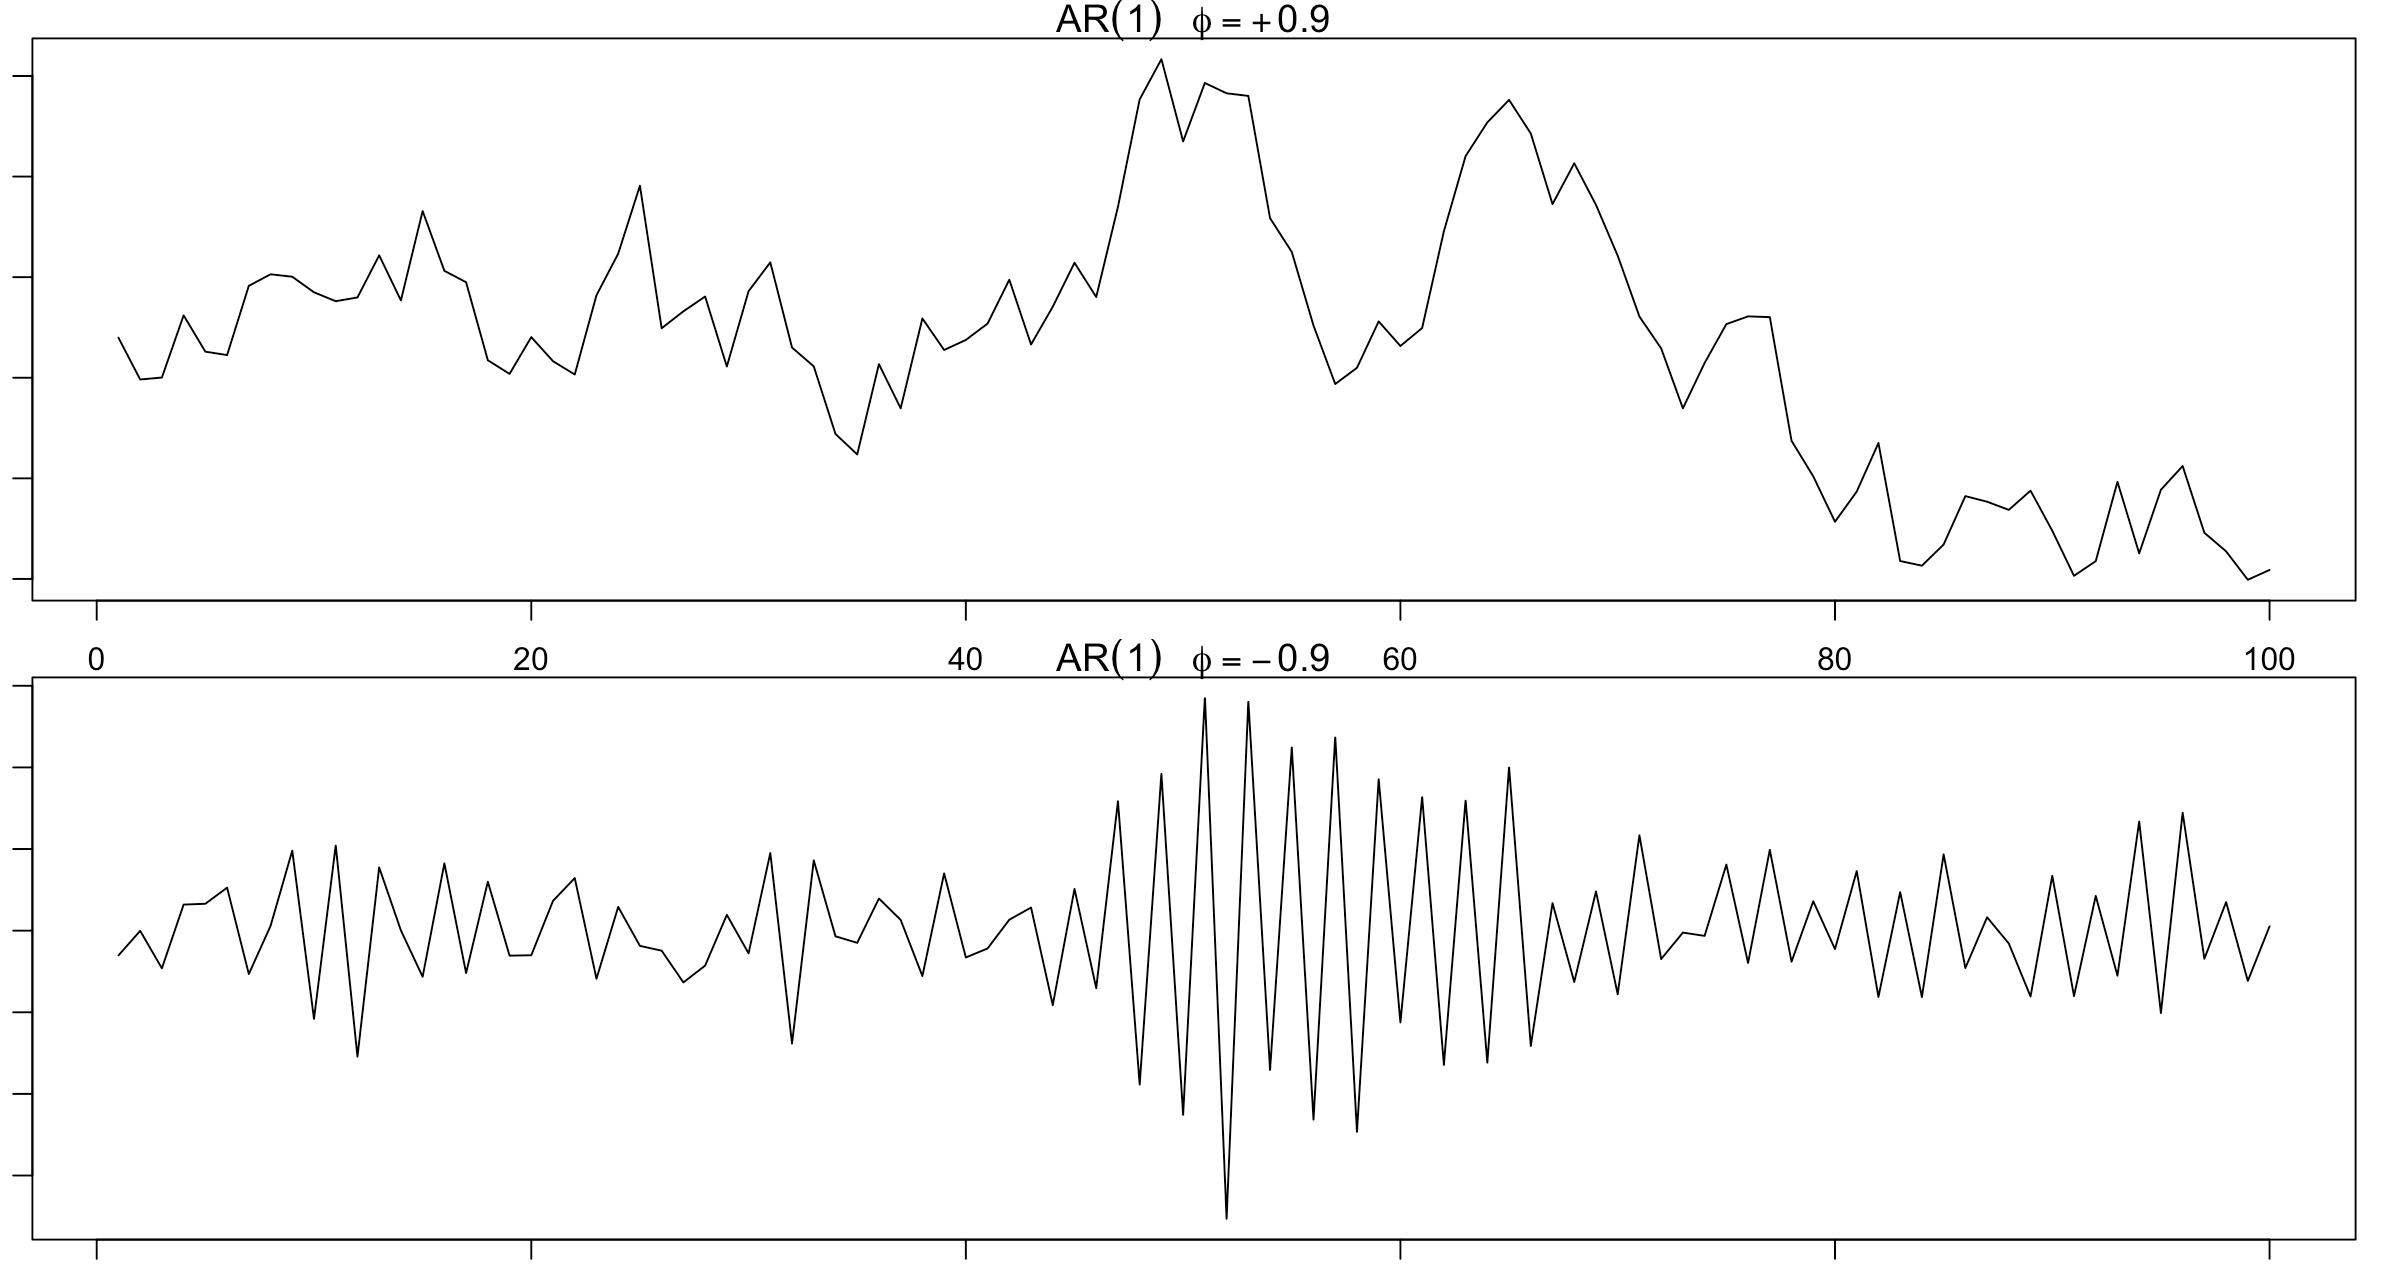
\includegraphics[width=\linewidth]{ar.png}}
	\caption{Simulaciones procesos AR(1): Arriba:$\phi=+0.9$.  Abajo: $\phi=-0.9$}\label{fig6}
\end{figure}

%\end{frame}

%---------------------------------------------------------
%---------------------Slide 28--------------------------
%\begin{frame}
%\frametitle{Identificaci\'on modelo AR(1) }
\subsection{Identificaci\'on modelo AR(1)}

Para el caso de un proceso del tipo AR, el correlograma, representaci\'on gr\'afica de la funci\'on de autocorrelaci\'on, tendr\'a un
comportamiento amortiguado hacia cero con todos los valores positivos, en caso de que $\theta > 0$, o bien alternando el signo, comenzando con negativo, si  $\theta < 0$.

\begin{figure}[H]
	\centering
	\textbf{Proceso Autoregresivo: AR(1)}\par\medskip
	\fcolorbox{green}{blue}{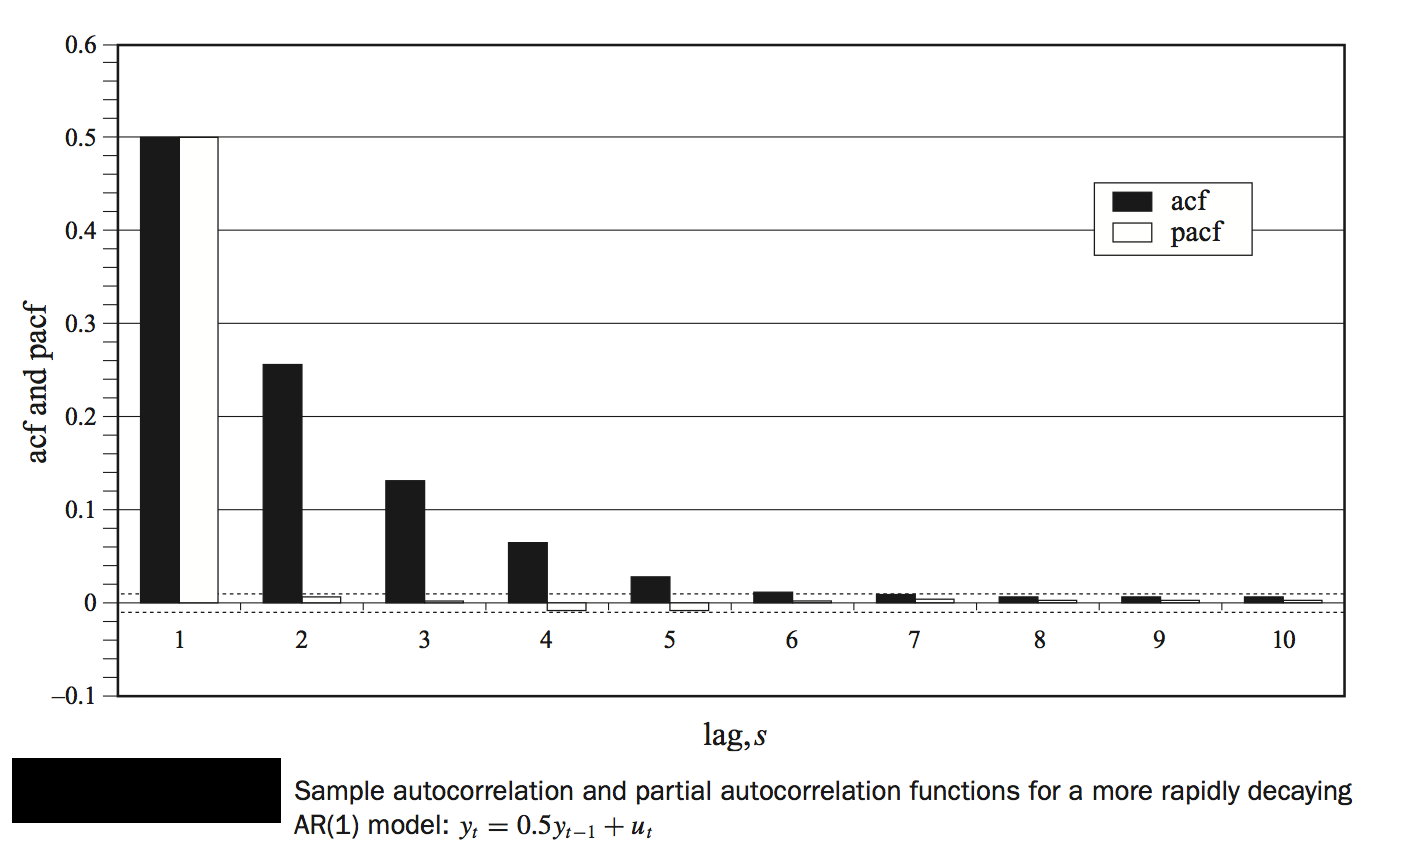
\includegraphics[width=\linewidth]{ar1corr.png}}
	\caption{Autocorrelogramas para autocorrelación(acf) y autocorrelación parcial(pacf)}\label{fig7}
\end{figure}


%\end{frame}
%---------------------------------------------------------
%---------------------Slide 29--------------------------
%\begin{frame}
%\frametitle{Identificaci\'on modelo AR(1) }

\begin{figure}[H]
		\centering
		\textbf{Proceso Autoregresivo: AR(1)}\par\medskip
		\fcolorbox{green}{blue}{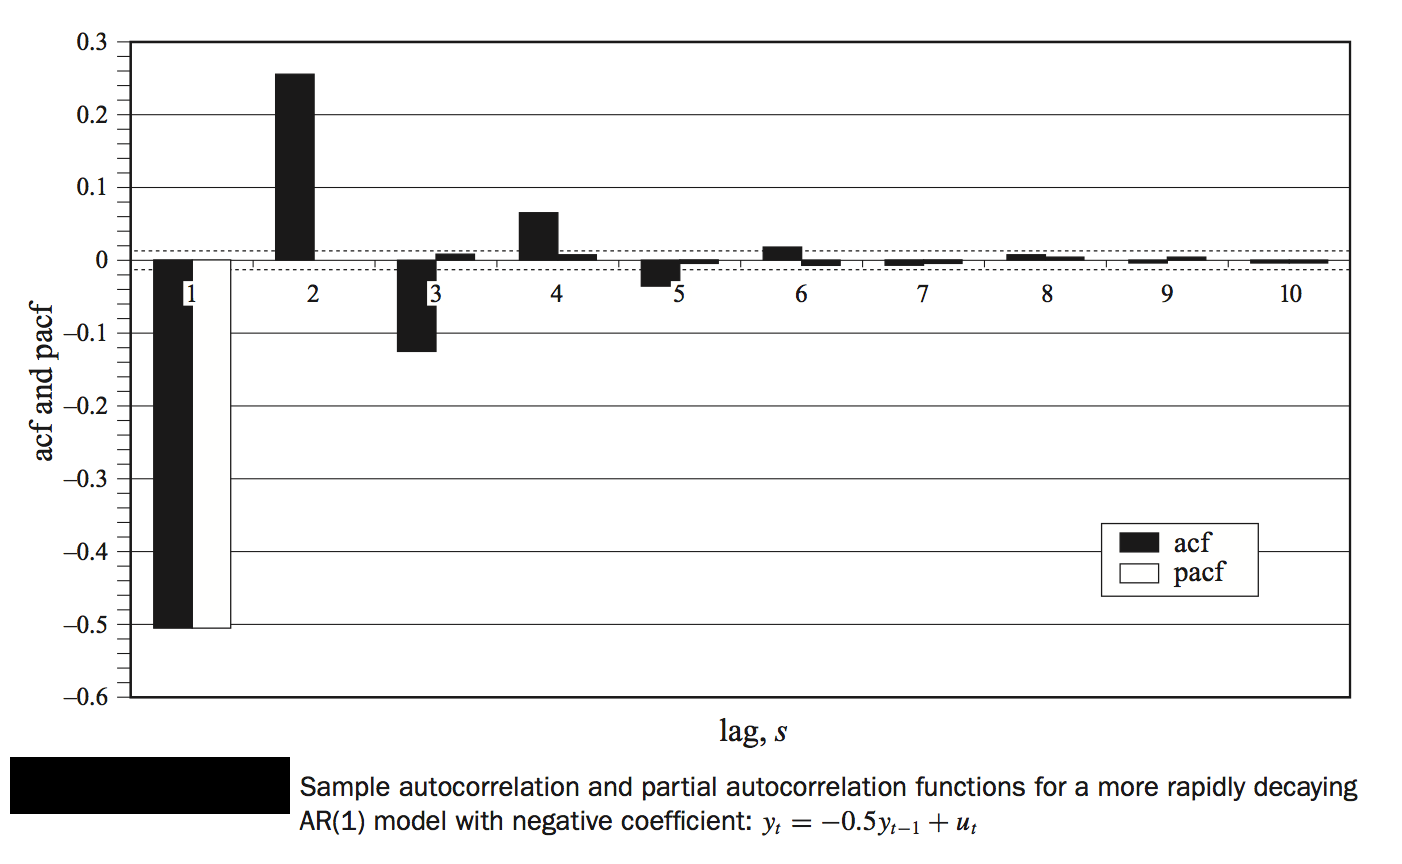
\includegraphics[width=\linewidth]{ar1corrb.png}}
		\caption{Autocorrelogramas para autocorrelación(acf) y autocorrelación parcial(pacf)}\label{fig8}

\end{figure}

%\end{frame}
%---------------------------------------------------------
%---------------------Slide 30--------------------------
%\begin{frame}
%\frametitle{Modelos ARIMA: modelando el corto plazo}

%\textbf{Media M\'ovil - MA (q)}
\pagebreak
\subsection{Media M\'ovil - MA (q)}

Como una alternativa a la representaci\'on autorregresiva en la que se supone que el $x_t$ en el lado izquierdo de la ecuaci\'on se combina linealmente, el modelo de promedio m\'ovil de orden q, abreviado como $MA (q)$, asume que el ruido blanco $\epsilon_t$ usualmente a la mano derecha de la ecuaci\'on, se combinan linealmente para modelar los datos observados.
%\end{frame}

%---------------------------------------------------------
%---------------------Slide 31--------------------------
%\begin{frame}
%\frametitle{Modelos ARIMA: modelando el corto plazo}
%
%\only<1|handout:1>{
%	\begin{block}{Definici\'on: Media M\'ovil - $MA (q)$}
%		
%		\begin{equation}
%		x_t = \epsilon_t + \theta_1 \epsilon_{t-1} +  \theta_2 \epsilon_{t-2} + \dots{} +  \theta_q \epsilon_{t-q} 
%		\end{equation}
%		
%		donde hay $q$ rezagos de la media m\'ovil $\epsilon_t$ y $\theta_1$  + $ \theta_2$ + $\dots{}$ + $ \theta_q$ son par\'ametros. \\
%		\vspace{4mm}	
%		Aunque no es necesario, suponemos que $\epsilon_t$ es una serie de ruido blanco.
%		
%	\end{block}
%}

\begin{mdframed}[style=MyFrame]
	\begin{definition}\label{def5}
		\textbf{Definici\'on:  Media M\'ovil - $MA (q)$:}
		\begin{equation}
				x_t = \epsilon_t + \theta_1 \epsilon_{t-1} +  \theta_2 \epsilon_{t-2} + \dots{} +  \theta_q \epsilon_{t-q} 
				\end{equation}
				
				donde hay $q$ rezagos de la media m\'ovil $\epsilon_t$ y $\theta_1$  + $ \theta_2$ + $\dots{}$ + $ \theta_q$ son par\'ametros. \\
				\vspace{4mm}	
				Aunque no es necesario, suponemos que $\epsilon_t$ es una serie de ruido blanco.
	\end{definition}
\end{mdframed}
%\end{frame}


%---------------------------------------------------------
%---------------------Slide 32--------------------------
%\begin{frame}
%\frametitle{Modelos ARIMA: modelando el corto plazo}

%\only<1|handout:1>{
%\begin{block}{Definici\'on: Media M\'ovil - $MA (q)$}
%	
%%	Tambi\'en podemos escribir el proceso $MA (q)$ en la forma equivalente:
%%	
%%	\begin{equation}
%%	x_t = \theta_t (B) \epsilon_{t} 
%%	\end{equation}
%%	
%%	donde  $\theta_t$ es el operador de promedio m\'ovil definido como:
%%	
%%	\begin{equation}
%%	\theta (B) = 1 + \theta_1B + \theta_2B^2 + \dots{} + \theta_q B^q
%%	\end{equation}
%%	\\
%%	\vspace{4mm}	
%%	A diferencia del proceso autorregresivo, el proceso de promedio m\'ovil es estacionario para cualquier valor de los par\'ametros $\theta_1$ + $\theta_2$ +$ \dots{}$ + $\theta_q$.
%	
%	
%\end{block}
%}
\pagebreak
\begin{mdframed}[style=MyFrame]
	\begin{definition}\label{def6}
		\textbf{Definici\'on:  Media M\'ovil - $MA (q)$:}
			Tambi\'en podemos escribir el proceso $MA (q)$ en la forma equivalente:
		
		\begin{equation}
		x_t = \theta_t (B) \epsilon_{t} 
		\end{equation}
		
		donde  $\theta_t$ es el operador de promedio m\'ovil definido como:
		
		\begin{equation}
		\theta (B) = 1 + \theta_1B + \theta_2B^2 + \dots{} + \theta_q B^q
		\end{equation}
		\\
		\vspace{4mm}	
		A diferencia del proceso autorregresivo, el proceso de promedio m\'ovil es estacionario para cualquier valor de los par\'ametros $\theta_1$ + $\theta_2$ +$ \dots{}$ + $\theta_q$.
		
	\end{definition}
\end{mdframed}
%\end{frame}


%---------------------------------------------------------
%---------------------Slide 33--------------------------
%\begin{frame}
%\frametitle{Modelos ARIMA: modelando el corto plazo}

%\textbf{Interpretaci\'on del model de media m\'ovil - MA (q)}
\subsubsection[1]{Interpretaci\'on del model de media m\'ovil - MA (q)}

As\'{\i} como un modelo autorregresivo es intuitivamente sencillo de comprender, la formulaci\'on de un modelo de medias m\'oviles resulta frecuentemente no intuitivo. ?`Qu\'e significa que una variable aleatoria se explique en funci\'on de los errores cometidos en per\'{\i}odos anteriores?, ?`De d\'onde vienen esos errores?, ?`Cu\'al es la justificaci\'on de un modelo de este tipo?.
En realidad, un modelo de medias m\'oviles puede obtenerse a partir de un modelo autorregresivo a partir de la realizaci\'on de sucesivas sustituciones.

%\end{frame}

%---------------------------------------------------------
%---------------------Slide 34--------------------------
%\begin{frame}
%\frametitle{Modelos ARIMA: modelando el corto plazo}

%\textbf{Interpretaci\'on del model de media m\'ovil - MA (q)}
\subsubsection[2]{Interpretaci\'on del model de media m\'ovil - MA (q)}
Supongamos un modelo $AR(1)$, sin t\'ermino independiente:

\begin{equation}
x_t =  \phi x_{t-1} + \epsilon_t
\end{equation}

si consideramos $t-1$ en lugar de $t$ el modelo ser\'{\i}a en este caso:

\begin{equation}
x_{t-1} =  \phi x_{t-2} + \epsilon_{t-1}
\end{equation}

sustituyendo:

\begin{equation}
x_t =  \phi^2 x_{t-2} + \phi \epsilon_{t-1} + \epsilon_t
\end{equation}

%\end{frame}

%---------------------------------------------------------
%---------------------Slide 35--------------------------
%\begin{frame}
%\frametitle{Modelos ARIMA: modelando el corto plazo}
%
%\textbf{Interpretaci\'on del model de media m\'ovil - MA (q)}

si ahora sustituimos $x_{t-2}$ por su expresi\'on autorregresiva y as\'{\i} sucesivamente llegamos a un modelo del tipo:

\begin{equation}
x_t = \epsilon_t + \theta \epsilon_{t-1} +  \theta^2 \epsilon_{t-2} + \dots{} +  \theta^q \epsilon_{t-q} 
\end{equation}

que es la expresi\'on, sin t\'ermino independiente, de un modelo de medias m\'oviles como el planteado anteriormente. En realidad, de forma estricta, el paso de un modelo a otro deber\'{\i}a realizarse al contrario, de un MA a un AR, utilizando el teorema general de descomposici\'on de Wold.

%\end{frame}

%---------------------------------------------------------
%---------------------Slide 36 --------------------------
%\begin{frame}
%\frametitle{Simulaci\'on modelo MA(1) }

%\only<1|handout:1>{
%\begin{exampleblock}{C\'odigo en R}
%par(mfrow = c(2,1))\\
%plot(arima.sim(list(order=c(0,0,1), ma=.5), n=100), ylab=``x",\\
%main=(expression(MA(1)~~~theta==+.5)))\\
%plot(arima.sim(list(order=c(0,0,1), ma=-.5), n=100), ylab=``x",\\
%main=(expression(MA(1)~~~theta==-.5)))\\
%\end{exampleblock}
%}
\lstset{caption=Ejemplo Simulaci\'on modelo MA(1) ,framexleftmargin=5mm, frame=shadowbox, rulesepcolor=\color{green}}
\begin{lstlisting}[title={‘Código R: ejemplo Simulaci\'on modelo MA(1) ’},basicstyle=\ttfamily]{}
par(mfrow = c(2,1))
plot(arima.sim(list(order=c(0,0,1), ma=.5), n=100), ylab="x",
main=(expression(MA(1), theta==+.5)))
plot(arima.sim(list(order=c(0,0,1), ma=-.5), n=100), ylab="x",
main=(expression(MA(1), theta==-.5)))
\end{lstlisting}
%\end{frame}
%---------------------------------------------------------
%---------------------Slide 37--------------------------
%\begin{frame}
%\frametitle{Simulaci\'on modelo MA(1) }

\begin{figure}[H]
	\centering
	\textbf{Ejemplo 1: Simulaci\'on modelo MA(1)}\par\medskip
	\fcolorbox{green}{blue}{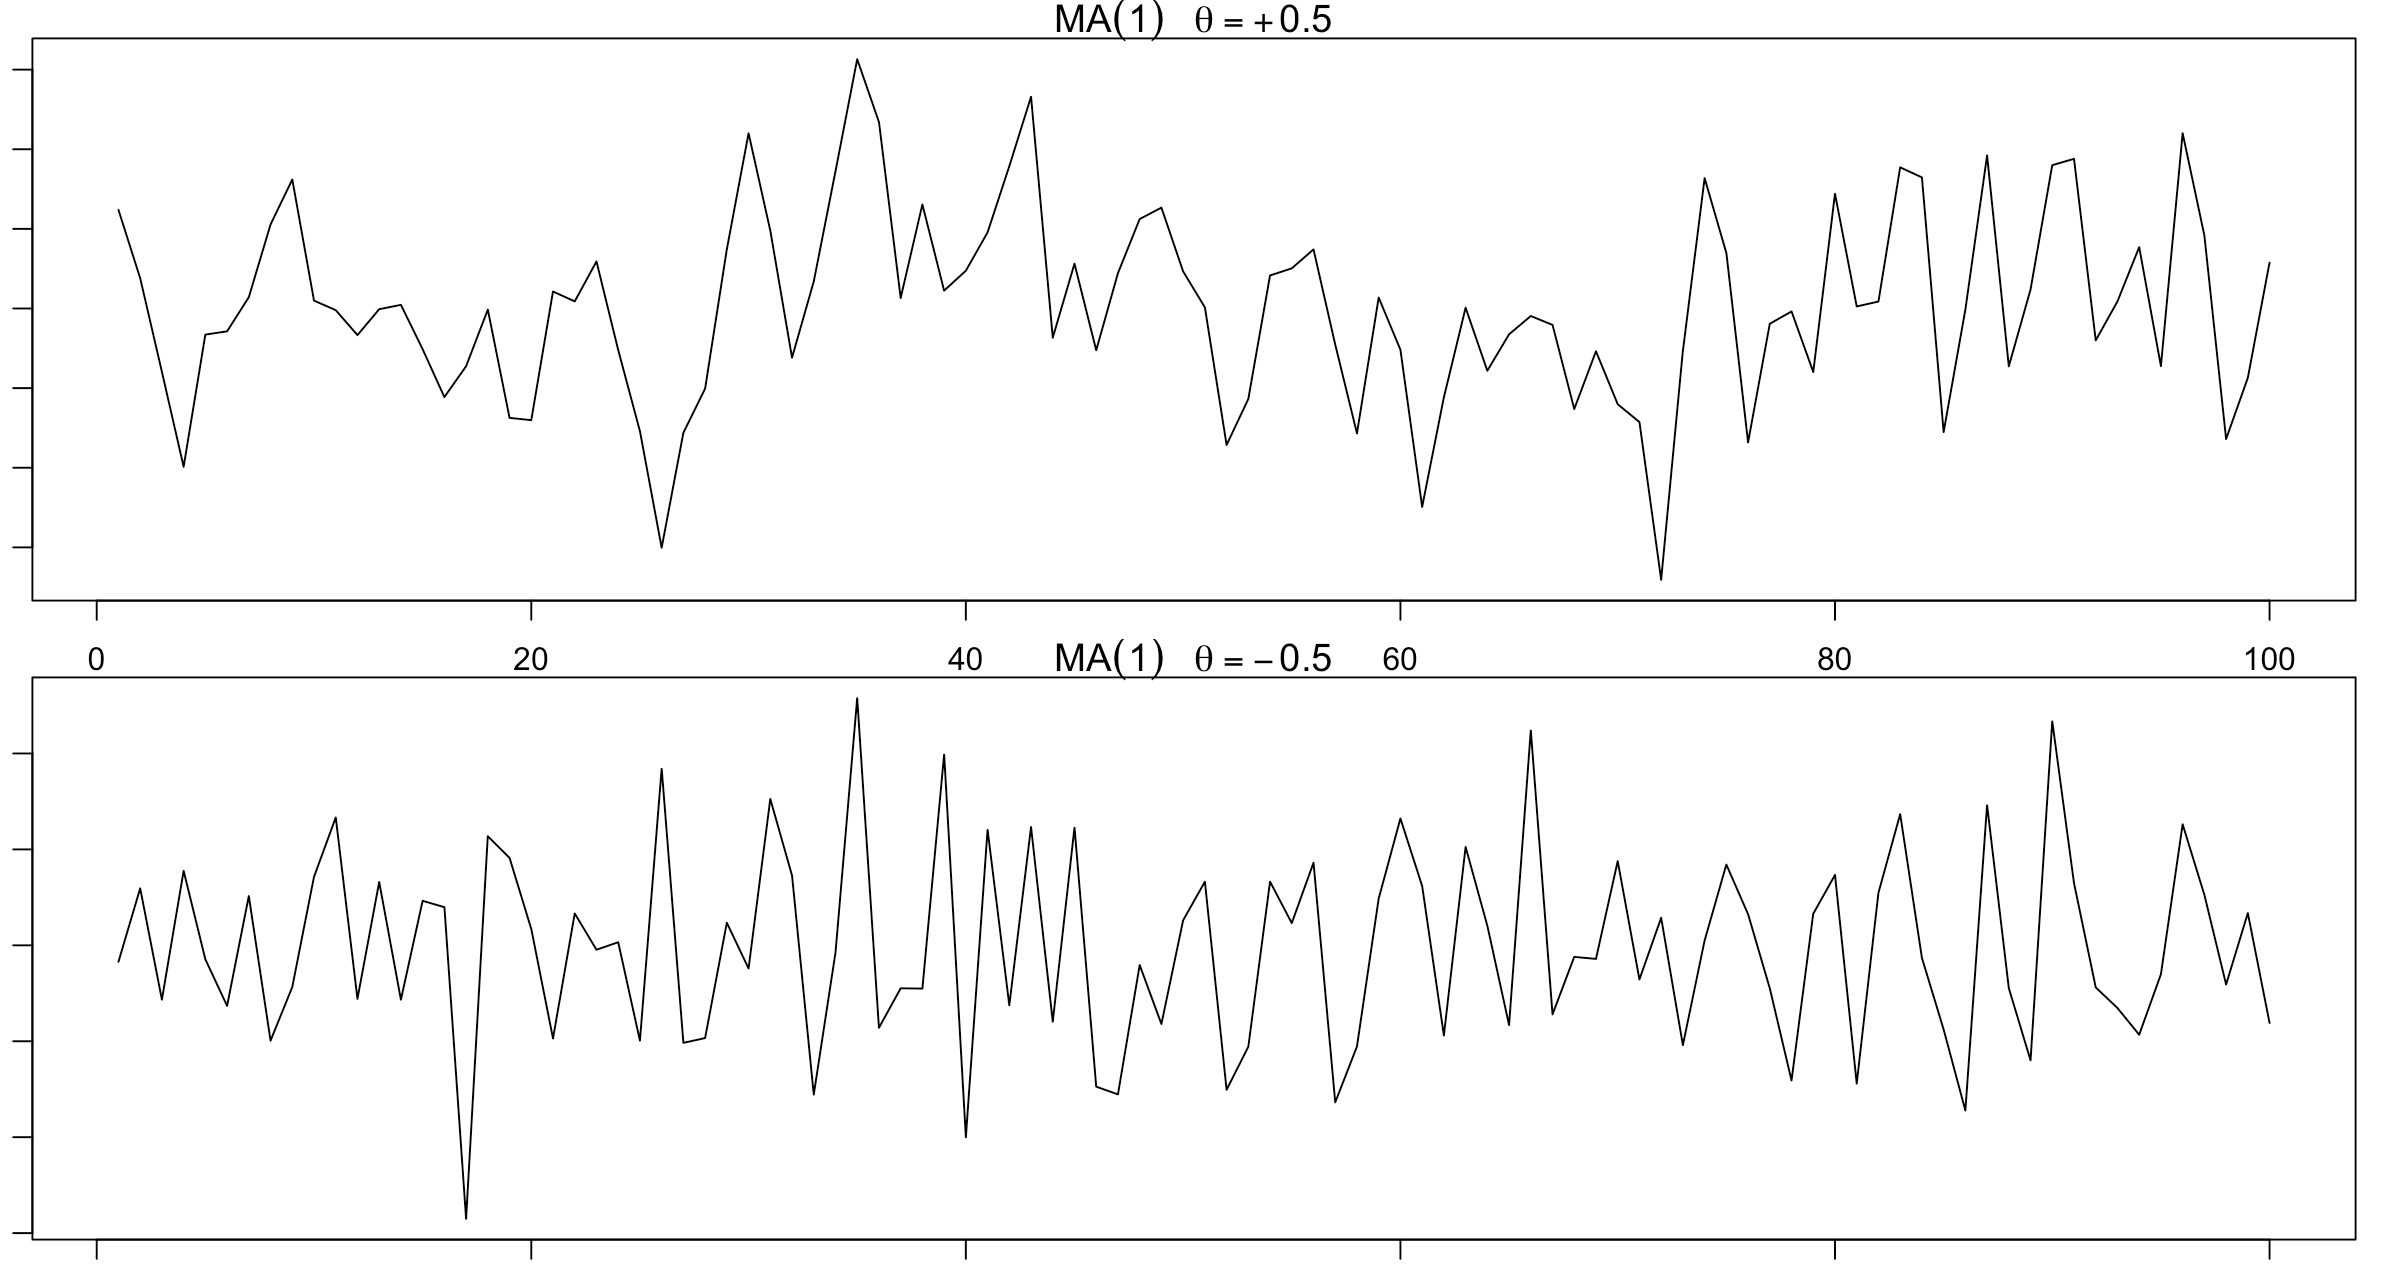
\includegraphics[width=\linewidth]{ma.png}}
	\caption{Procesos de medias móviles. Arriba: parámetro $\theta=+0.5$. Abajo: parámetro $\theta=-0.5$}\label{fig9}
\end{figure}

%\end{frame}

%---------------------------------------------------------
%---------------------Slide 38--------------------------
%\begin{frame}
%\frametitle{Identificaci\'on modelo MA }
\pagebreak
\subsubsection{Identificaci\'on modelo MA }
Para la identificaci\'on de todos los componentes del modelo MA, tal como vimos para el modelo AR, se utiliza la funci\'on de autocorrelaci\'on (AFC) y la funci\'on de autocorrelaci\'on parcial (PAFC), y as\'{\i} se procede a la identificaci\'on de los componentes, en base a los gr\'aficos de los distintos modelos te\'oricos.

\begin{figure}[H]
	\centering
	\textbf{Autocorrelograma de proceso de media móvil MA(1), $\theta=+0.5$}\par\medskip
	\fcolorbox{green}{blue}{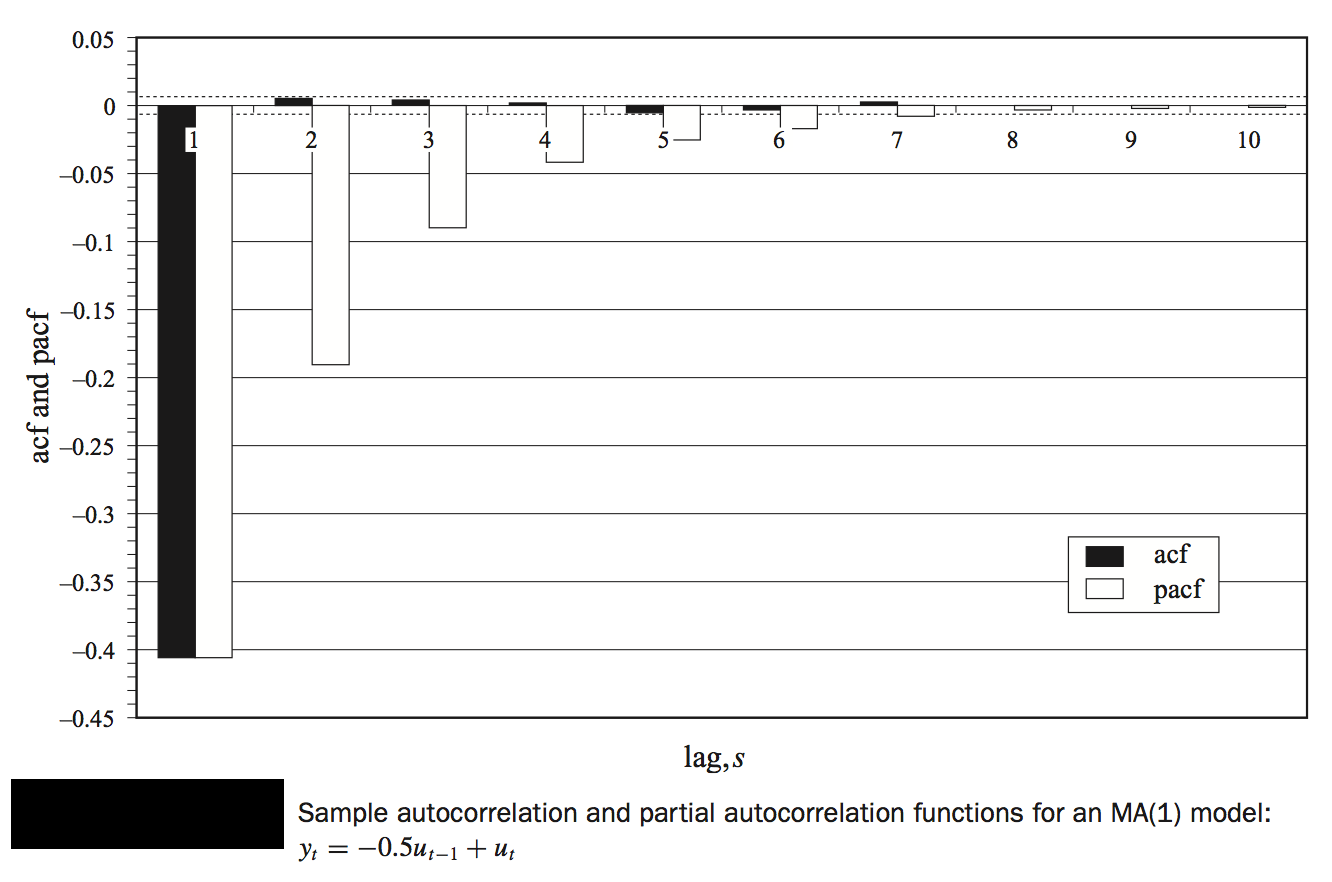
\includegraphics[scale=0.3]{idMA1.png}}
	\caption{Autocorrelogramas para diferentes retardos de proceso de media móvil con $\theta=+0.5$(lags). ACF(barras negras), PACF(barras blancas).}\label{fig10}
\end{figure}


%\end{frame}
%---------------------------------------------------------
%---------------------Slide 39--------------------------
%\begin{frame}
%\frametitle{Identificaci\'on modelo ARMA }
\subsection{Identificaci\'on modelo ARMA}


\begin{figure}[H]
	\centering
	\textbf{Autocorrelograma de proceso de media móvil MA(1), $\theta=-0.5$ }\par\medskip
	\fcolorbox{green}{blue}{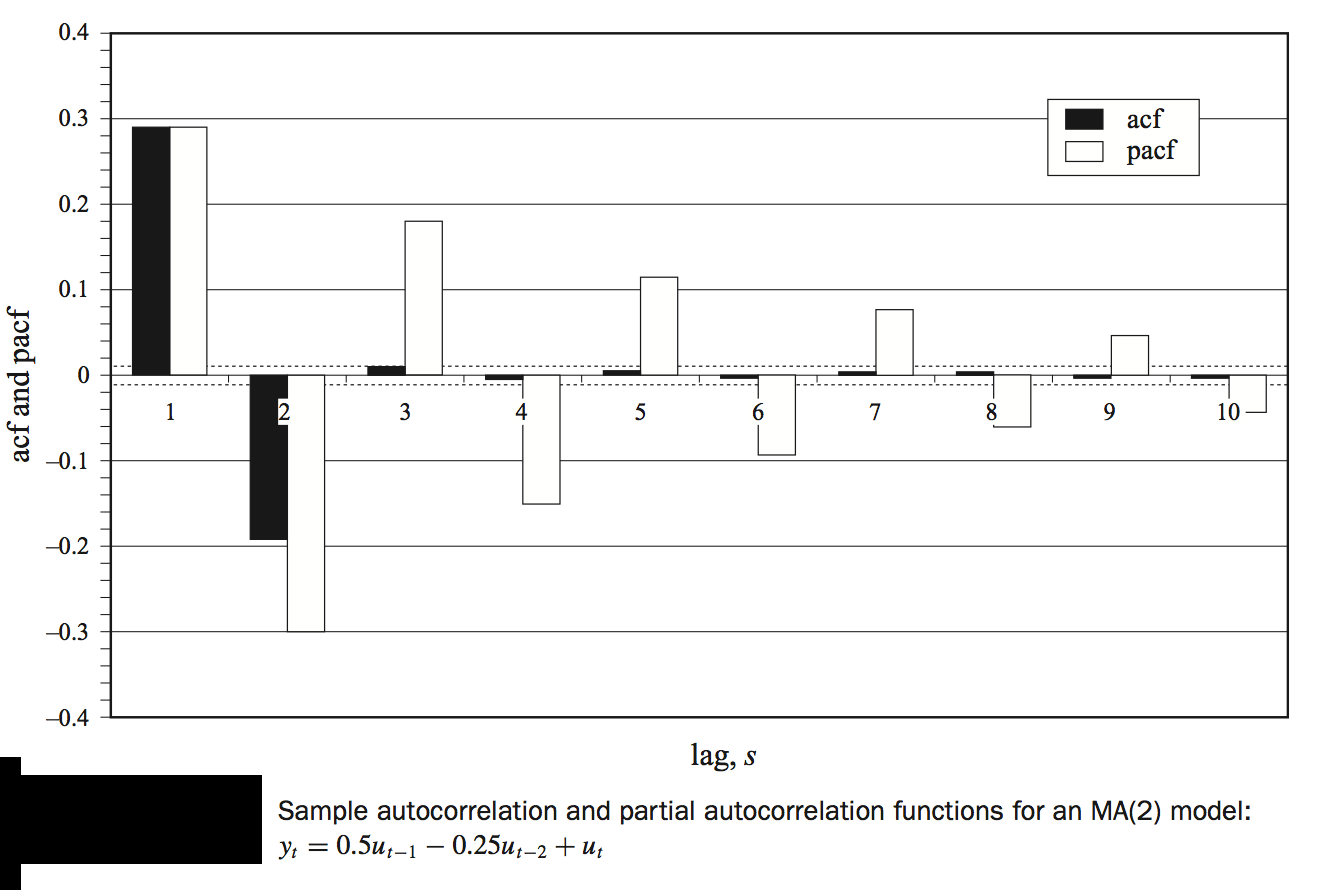
\includegraphics[width=\linewidth]{idMA2.png}}
	\caption{Autocorrelogramas para diferentes retardos de proceso de media móvil con $\theta=-0.5$(lags). ACF(barras negras), PACF(barras blancas).}\label{fig13}
\end{figure}


%\end{frame}
%---------------------------------------------------------
%---------------------Slide 40--------------------------
%\begin{frame}
%\frametitle{Modelos ARIMA: modelando el corto plazo}

%\only<1|handout:1>{
%\begin{block}{Definici\'on: Modelo ARMA - $ARMA (r,q)$}
%
%Una serie de tiempo $\{x_t, t = 0, \pm1, \pm2 , \dots{} \}$ es un proceso ARMA(p, q), si es estacionario y	
%\begin{equation}
%x_t =  \phi_1 x_{t-1} +  \phi_2 x_{t-2} + \dots{} +  \phi_p x_{t-p} + \epsilon_t + \theta_1 \epsilon_{t-1} +  \theta_2 \epsilon_{t-2} + \dots{} +  \theta_q \epsilon_{t-q} 
%\end{equation}
%
%Los par\'ametros p y q se llaman \'ordenes autoregresivas y promedios m\'oviles, respectivamente. \\
%\vspace{4mm}	
%Si $x_t$ tiene una media distinta de cero $\mu$, establecemos que $\alpha = \mu (1-\theta_1, \dots{} -\theta_q)$ y podemos re-escribimos el modelo como:
%
%\begin{equation}
%x_t = \alpha + \phi_1 x_{t-1} + \dots{} + \phi_p x_{t-p} + w_t +\theta_1  \epsilon_{t-1} + \dots{} + \theta_q  \epsilon_{t-q} .
%\end{equation}
%
%\end{block}
%}
\pagebreak
\begin{mdframed}[style=MyFrame]
	\begin{definition}\label{def7}
		\textbf{Definici\'on:  $Modelo ARMA - ARMA (r,q)$:}\\
Una serie de tiempo $\{x_t, t = 0, \pm1, \pm2 , \dots{} \}$ es un proceso ARMA(p, q), si es estacionario y	
\begin{equation}
x_t =  \phi_1 x_{t-1} +  \phi_2 x_{t-2} + \dots{} +  \phi_p x_{t-p} + \epsilon_t + \theta_1 \epsilon_{t-1} +  \theta_2 \epsilon_{t-2} + \dots{} +  \theta_q \epsilon_{t-q} 
\end{equation}

Los par\'ametros p y q se llaman \'ordenes autoregresivas y promedios m\'oviles, respectivamente. \\
\vspace{4mm}	
Si $x_t$ tiene una media distinta de cero $\mu$, establecemos que $\alpha = \mu (1-\theta_1, \dots{} -\theta_q)$ y podemos re-escribimos el modelo como:

\begin{equation}
x_t = \alpha + \phi_1 x_{t-1} + \dots{} + \phi_p x_{t-p} + w_t +\theta_1  \epsilon_{t-1} + \dots{} + \theta_q  \epsilon_{t-q} .
\end{equation}		
	\end{definition}
\end{mdframed}
%\end{frame}
%---------------------------------------------------------
%---------------------Slide 41 --------------------------
%\begin{frame}
%\frametitle{Modelos ARIMA: modelando el corto plazo}

%\textbf{Invertibilidad}
\subsection{Invertibilidad}
Una serie temporal es invertible si los errores se pueden invertir en una representaci\'on de observaciones pasadas. As\'{\i} por ejemplo, como ya vimos, el modelo AR es siempre invertible.
En el caso del modelo ARMA, las ra\'{\i}ces de las siguientes ecuaciones deben ser analizadas para garantizar invertibilidad.

\begin{equation}
\phi (z) = 1 + \phi_1 z + \phi_2 z^2 + \dots{} + \phi_p z^p
\end{equation}

\begin{equation}
\theta(z) =  1 + \theta_1 z + \theta_2 z^2 + \dots{} + \theta_q z^q
\end{equation}

En particular el modelo ARMA ser\'a invertible si y solo si $\theta(z) \ne 0$ para $|z| \le 1$
En general, los valores propios son la soluci\'on del $det (A - \lambda I)$ = 0, vemos que este es casi el polinomio caracter\'{\i}stico de las ecuaciones que definimos arriba. Por lo tanto, vemos que los valores propios de A son el inverso de las ra\'{\i}ces del polinomio caracter\'{\i}stico, y esa convergencia de la iteraci\'on hacia atr\'as ocurre cuando las ra\'{\i}ces del polinomio caracter\'{\i}stico se encuentran fuera del c\'{\i}rculo unitario.

%\end{frame}
%---------------------------------------------------------
%---------------------Slide 42 --------------------------
%\begin{frame}
%\frametitle{Modelos ARIMA: modelando el corto plazo}

%\textbf{Estacionaridad e Invertibilidad}
\subsection{Estacionaridad e Invertibilidad}
Wold demostr\'o que todos los procesos estoc\'asticos estacionarios de covarianza podr\'{\i}an descomponerse como la suma de
procesos determin\'{\i}sticos y linealmente indeterministas los cuales no estaban correlacionados con todos los rezagos; es decir,
si $y_t$ es la covarianza estacionaria, entonces:

\begin{equation}
y_t = x_t + z_t
\end{equation}

donde $x_t$ es un proceso determinista estacionario en covarianza y $z_t$ es linealmente indeterminista,
con $Cov (x_t, z_s) = 0$ para todas los $t$ y $s$. Este resultado proporciona una base te\'orica para la propuesta de Box y Jenkins  para modelar procesos estacionarios de covarianza escalar (desestacionalizados) como son los procesos ARMA.
%\end{frame}
%---------------------------------------------------------
%---------------------Slide 43--------------------------
%\begin{frame}
%\frametitle{Modelos ARIMA: modelando el corto plazo}

%\textbf{Modelos ARMA (p,q)}
\subsection{Modelos ARMA (p,q)}

Como se indic\'o anteriormente, cuando $q$ = 0, el modelo se denomina modelo autoregresivo de orden $p$, $AR (p)$, y cuando $p$ = 0, el modelo se denomina modelo de promedio m\'ovil de orden $q$, $MA (q)$. \\
Es \'util escribir los modelos ARIMA usando el operador AR y el operador MA descritos anteriormente. En particular, el modelo $ARMA (p, q) $ puede escribirse entonces en forma concisa como:

\begin{equation}
\phi (B) x_t = \theta (B) \epsilon_t.
\end{equation}
%\textbf{Modelos ARIMA (p, i, q)}
\subsection{Modelos ARIMA (p, i, q)}
El modelo ARMA gana su I y se convierte en ARIMA cuando debe ser integrado para lograr estacionaridad. El \'{\i}ndice $I$ ser\'a entonces el numero de veces que debe ser diferenciado.
%\end{frame}

%---------------------------------------------------------
%---------------------Slide 44--------------------------
%\begin{frame}
%\frametitle{Identificaci\'on modelo ARMA }
\subsection{Identificaci\'on modelo ARMA}

Para la identificaci\'on de todos los componentes del modelo ARMA se utiliza la funci\'on de autocorrelaci\'on (AFC) y la funci\'on de autocorrelaci\'on parcial (PAFC), y as\'{\i} se procede a la identificaci\'on de los componentes estacional y no estacional por separado, en base a los gr\'aficos de los distintos modelos te\'oricos.

\begin{figure}[H]
	\centering
	\textbf{Proceso autoregresivo de media móvil de orden (1,1): ARMA(1,1)}\par\medskip
	\fcolorbox{green}{blue}{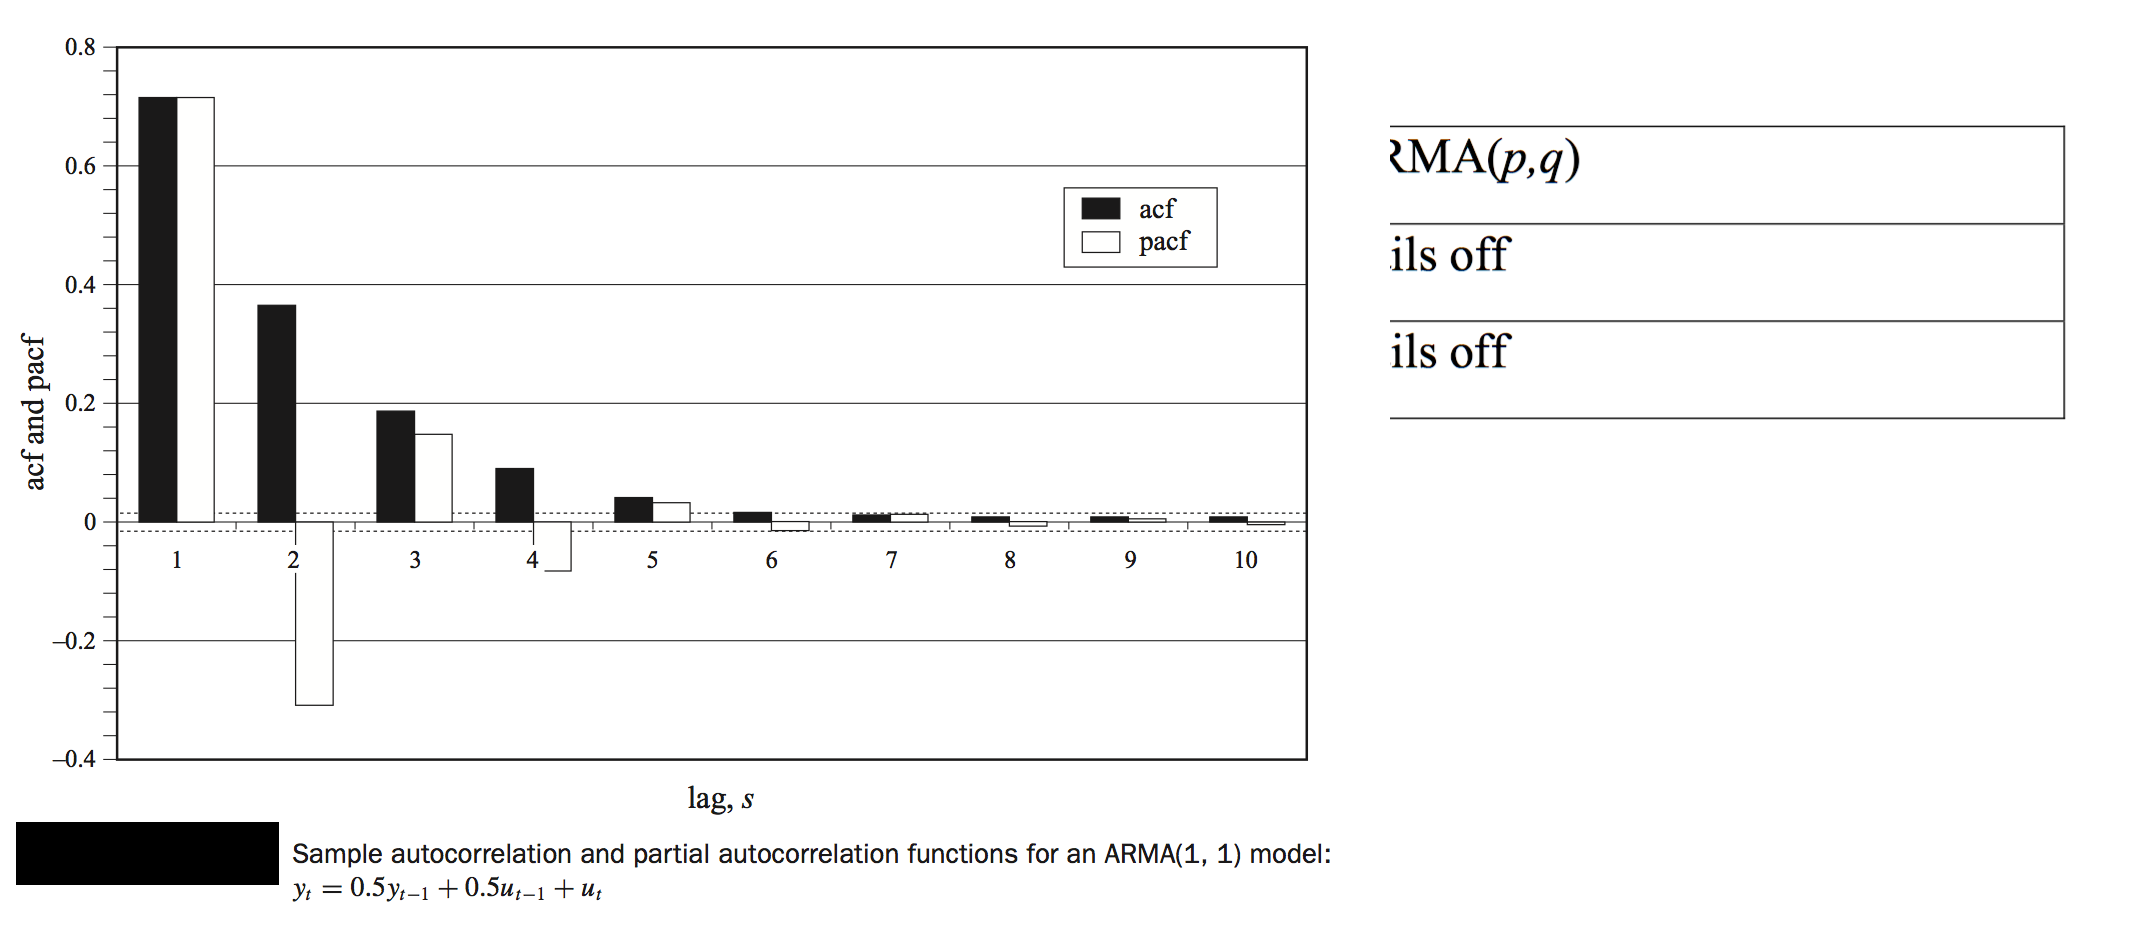
\includegraphics[width=\linewidth]{idARMA.png}}
	\caption{Autocorrelogramas para diferentes retardos(lags) para un proceso ARMA(1,1)}\label{fig16}
\end{figure}

%\end{frame}
%---------------------------------------------------------
%---------------------Slide 45--------------------------
%\begin{frame}
%\frametitle{Identificaci\'on modelo ARMA }

En resumen tendremos:

\begin{figure}[H]
	\centering
	\textbf{En resumen tendremos:}\par\medskip
	\fcolorbox{green}{blue}{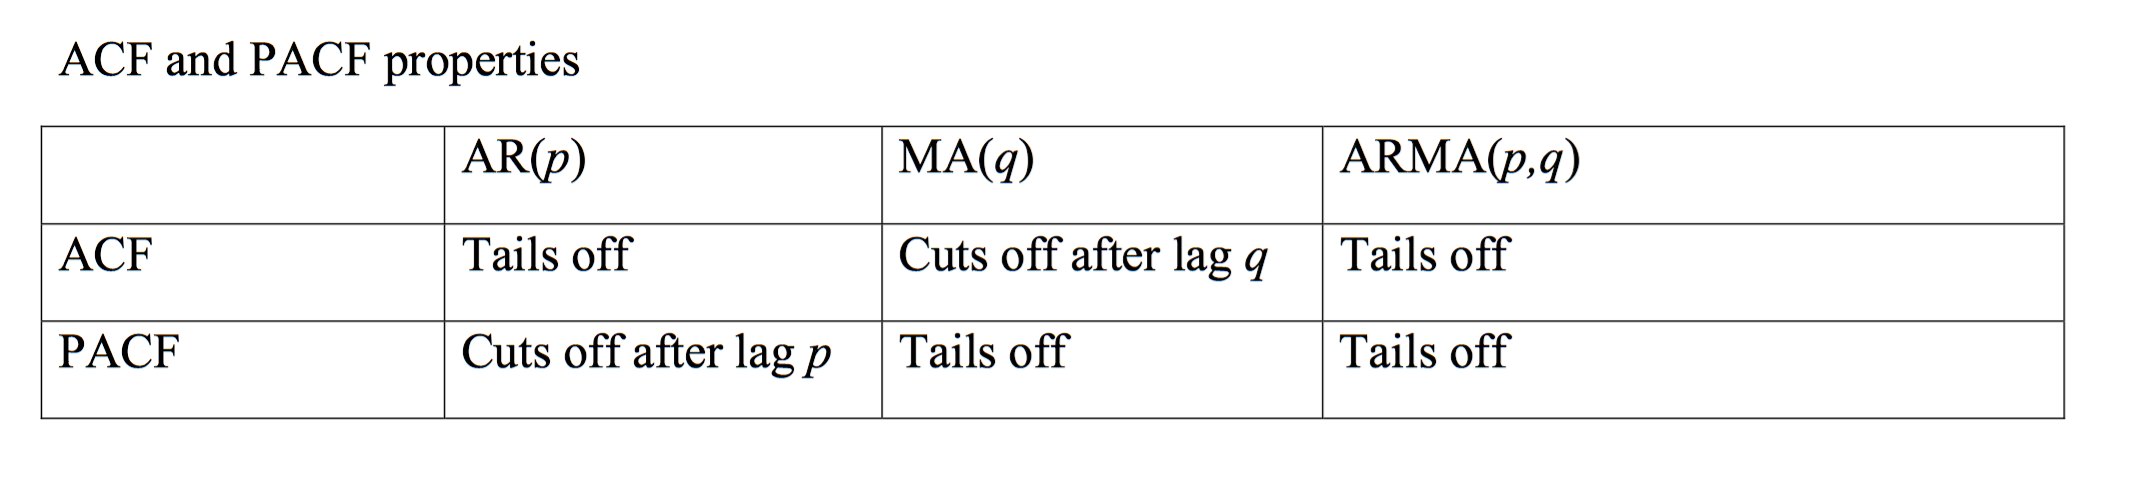
\includegraphics[width=\linewidth]{resumenARMA.png}}
	\caption{Tabla resumen de los modelos AR(p),MA(q) y ARMA(p,q), con sus respectivos resultados esperados para las funciones de autocorrelación(ACF) y autocorrelación parcial(PACF)}\label{fig14}
\end{figure}

%\end{frame}
%---------------------------------------------------------
%---------------------Slide 46--------------------------
%\begin{frame}
%\frametitle{Modelos SARIMA (p,q)}
\subsection{Modelos SARIMA (p,q)}

Los modelos ARIMA tambi\'en son capaces de modelar una amplia gama de datos estacionales. Los llamados  modelos SARIMA, Seasonal ARIMA models, se obtienen al incluir t\'erminos estacionales adicionales en los modelos ARIMA que hemos visto hasta ahora, de la siguiente manera:

\begin{equation}
ARIMA (p,d,q)(P,D,Q)m
\end{equation}

donde m = n\'umero de per\'{\i}odos por temporada. \\
Usamos la notaci\'on en may\'usculas para las partes estacionales del modelo y la notaci\'on en min\'usculas para las partes no estacionales del modelo.\\
La parte estacional del modelo consiste en t\'erminos que son muy similares a los componentes no estacionales del modelo, pero implican retrocesos del per\'{\i}odo estacional. \\

%\end{frame}
%\end{section}
%---------------------------------------------------------
%---------------------Slide 47--------------------------
%\begin{section}{Evaluaci\'on estad\'{\i}stica de un Modelo ARIMA}
%\begin{frame}
%\frametitle{Evaluaci\'on estad\'{\i}stica de un Modelo ARIMA}
\subsubsection[evaluación]{Evaluaci\'on estad\'{\i}stica de un Modelo ARIMA}
Se debe evaluar:
%\only<1->{
\begin{itemize}
\item[A] \textbf{Significancia estad\'{\i}stica de los par\'ametros} 
Los coeficientes obtenidos en la estimaci\'on que no sean significativamente distintos de cero, a un nivel de significancia del $5\%$, no son necesarios, por lo que deben eliminarse.
\item[B] \textbf{Estacionariedad e invertibilidad del modelo estimado.} Para valores de los coeficientes estimados pr\'oximos a la frontera de la no-estacionariedad, es conveniente llevar a cabo un test de ra\'{\i}ces unitarias.
\item[C] \textbf{Estabilidad del modelo estimado.} Aunque los par\'ametros sean significativos, el modelo puede ser rechazado si existe una fuerte correlaci\'on entre los par\'ametros del modelo. Esto ocurre cuando el coeficiente de correlaci\'on tiene un valor absoluto superior a 0,7, entonces es conveniente probar con modelos alternativos.
\end{itemize}
%} 

%\end{frame}

%---------------------------------------------------------
%---------------------Slide 48--------------------------
%\begin{frame}
%\frametitle{Sobre la Selecci\'on de Modelos}
\subsection{Sobre la Selecci\'on de Modelos}

Puede ocurrir que varios modelos describan satisfactoriamente la serie temporal, por lo que sea necesario seleccionar el modelo m\'as adecuado. Este proceso de selecci\'on puede ser sencillo o un poco m\'as complejo, por lo que es necesario recurrir a criterios de selecci\'on de modelos.\\
%\par
Los criterios m\'as comunes en la selecci\'on de modelos son el AIC (Akaike Information Criterion) y el BIC (Bayesian Information Criterion) que es una extensi\'on bayesiana del primero. 

%\end{frame}

%---------------------------------------------------------
%---------------------Slide 49 --------------------------
%\begin{frame}
%\frametitle{Criterios de Informaci\'on}
\subsubsection{Criterios de Informaci\'on}

%\only<1|handout:1>{
%\begin{block}{Definici\'on: Akaike Information Criterion}
%\begin{equation*}
%AIC = log \hat{\sigma_k^2} + \frac{n+2k}{n} 
%\end{equation*}
%\end{block}
%}
\begin{mdframed}[style=MyFrame]
	\begin{definition}\label{def8}
		\textbf{Definici\'on: Akaike Information Criterion}
		\begin{equation*}
		AIC = log \hat{\sigma_k^2} + \frac{n+2k}{n} 
		\end{equation*}
	\end{definition}
\end{mdframed}
\vspace{4mm}	
Donde $\hat{\sigma_k^2} = \frac{SSE_k}{n}$, donde $k$ es el n\'umero de par\'ametros del modelo, $n$ el tama\~no de la muestra, y $SSE_k$ equivale a la suma de los residuos al cuadrado bajo el modelo $k$ ($SSE_k=\sum_{t=1}^{n}(x_t-\bar{x})^2$).\\
%\par
%\vspace{4mm}	
El valor de $k$ que produce el m\'{\i}nimo AIC representa el mejor modelo. La idea es que minimizar $\hat{\sigma_k^2}$ representa un objetivo razonable, excepto que disminuye mon\'otonamente a medida que $k$ aumenta. Por lo tanto, debemos penalizar la varianza del error por un t\'ermino proporcional al n\'umero de par\'ametros.

%\end{frame}
%---------------------------------------------------------
%---------------------Slide 50 --------------------------
%\begin{frame}
%\frametitle{Criterios de Informaci\'on}
%
%\only<1|handout:1>{
%	\begin{block}{Definici\'on: Bias Corrected}
%		\begin{equation*}
%		AICc = log \hat{\sigma_k^2} + \frac{n+k}{n-k-2} 
%		\end{equation*}
%	\end{block}
%}
\begin{mdframed}[style=MyFrame]
	\begin{definition}\label{def15}
		\textbf{Definici\'on:  Bias Corrected}
		\begin{equation*}
				AICc = log \hat{\sigma_k^2} + \frac{n+k}{n-k-2} 
		\end{equation*}
	\end{definition}
\end{mdframed}

%\only<1|handout:1>{
%	\begin{block}{Definici\'on: Bayesian Information Criterion - BIC}
%		\begin{equation*}
%		AICc = log \hat{\sigma_k^2} + \frac{k log n}{n} 
%		\end{equation*}
%	\end{block}
%}
\begin{mdframed}[style=MyFrame]
	\begin{definition}\label{def16}
		\textbf{Definici\'on:  Bayesian Information Criterion - BIC}
		\begin{equation*}
		AICc = log \hat{\sigma_k^2} + \frac{k log n}{n} 
		\end{equation*}		
	\end{definition}
\end{mdframed}
BIC tambi\'en se conoce como el \textbf{Schwarz Information Criterion (SIC)}. Varios estudios de simulaci\'on han verificado que BIC es adecuado para obtener el orden correcto en muestras grandes, mientras que AICc tiende a ser superior en muestras m\'as peque\~nas donde el n\'umero relativo de par\'ametros es grande.

%\end{frame}

%---------------------------------------------------------
%---------------------Slide 51--------------------------
%\begin{frame}
%\frametitle{Sobre la Selecci\'on de Modelos}

\pagebreak En \'ultimo t\'ermino un modelo es mejor que otro si su predicci\'on es mejor. Por otro lado, diremos que \textbf{una predicci\'on, es mejor que otra, cuando comete un menor error extra-muestral.}\\
%\par
As\'{\i}, la precisi\'on de los m\'etodos utilizados para pronosticar se pueden medir por ejemplo a trav\'es de la funci\'on de p\'erdida: \textbf{Error cuadr\'atico medio - Mean Square Error (MSE)}, con el fin de comprender qu\'e modelo proporciona un mejor pron\'ostico extra-muestral sobre otro. Esto es:

\begin{equation}
\textbf{MSE}=\frac{1}{T} \sum_{t=1}^T (x_t-\hat{x}_t)^2
\label{MSE}
\end{equation}

donde $x_t$ corresponde al valor real de la serie en el tiempo $t$ y $\hat{x}_{t}$ corresponde al valor pronosticado por el modelo propuesto en el mismo instante.

%\end{frame}

%---------------------------------------------------------
%---------------------Slide 52--------------------------
%\begin{frame}
%\frametitle{Sobre la Selecci\'on de Modelos}

Otros criterios de selecci\'on de modelos que consideran el error extra-muestral son: 
\begin{itemize}
	\item i) el \textbf{Error Absoluto Medio (EAM) - mean absolute deviation (MAD)},
	\begin{equation}
	\textbf{MAD}=\frac{1}{T} \sum_{t=1}^T |x_t-\hat{x}_t|
	\label{MAD}
	\end{equation} y 
	\item ii) \textbf{Error Absoluto Porcentual Medio (EAPM) - mean absolute percentage error (MAPE)}
	\begin{equation}
	\textbf{MAPE}=\frac{1}{T} \sum_{t=1}^T \left| 1 - \frac{x_t}{\hat{x}_t}\right|
	\label{MAPE}
	\end{equation}
	 
\end{itemize}

%\begin{equation}
%\textbf{MAD}=\frac{1}{T} \sum_{t=1}^T |x_t-\hat{x}_t|
%\label{MAD}
%\end{equation}

%\begin{equation}
%\textbf{MAPE}=\frac{1}{T} \sum_{t=1}^T \left| 1 - \frac{x_t}{\hat{x}_t}\right|
%\label{MAPE}
%\end{equation}
%\end{frame}

%---------------------------------------------------------
%---------------------Slide 53 --------------------------
%\begin{frame}
%\frametitle{Ejemplo IPC en Chile}
\subsection{Ejemplo IPC en Chile}
Considerando data mensual del IPC desde enero del 2013 a la fecha en Chile, obtenida de la p\'agina del Banco Central, intetnaremos predecir el IPC (serie original).
%\only<1|handout:1>{
%\begin{exampleblock}{C\'odigo en R}
%rm(list=ls())\\
%data$<-$read.csv (``ipc.csv")\\
%ipc $<-$ ts(data[,2],start = c(2013,1), end=c(2018, 6), frequency = 12)\\
%plot.ts(ipc, xlab='Years', ylab = ``Indice de Precios al Comsumidor')\\
%
%\end{exampleblock}
%}
\lstset{caption=Ejemplo IPC en Chile ,framexleftmargin=5mm, frame=shadowbox, rulesepcolor=\color{green}}
\begin{lstlisting}[title={‘Código R: Ejemplo IPC en Chile’},basicstyle=\ttfamily]{}
rm(list=ls())
data<-read.csv ("ipc.csv")
ipc <- ts(data[,2],start = c(2013,1), end=c(2018, 6),
		frequency = 12)
plot.ts(ipc,xlab='Years',ylab='Indice de Precios al Comsumidor')
\end{lstlisting}
%\end{frame}
%---------------------------------------------------------
%---------------------Slide 54--------------------------
%\begin{frame}
%\frametitle{Ejemplo IPC en Chile}

\begin{figure}[H]
	\centering
	\textbf{Ejemplo IPC en Chile.}\par\medskip
	\fcolorbox{green}{blue}{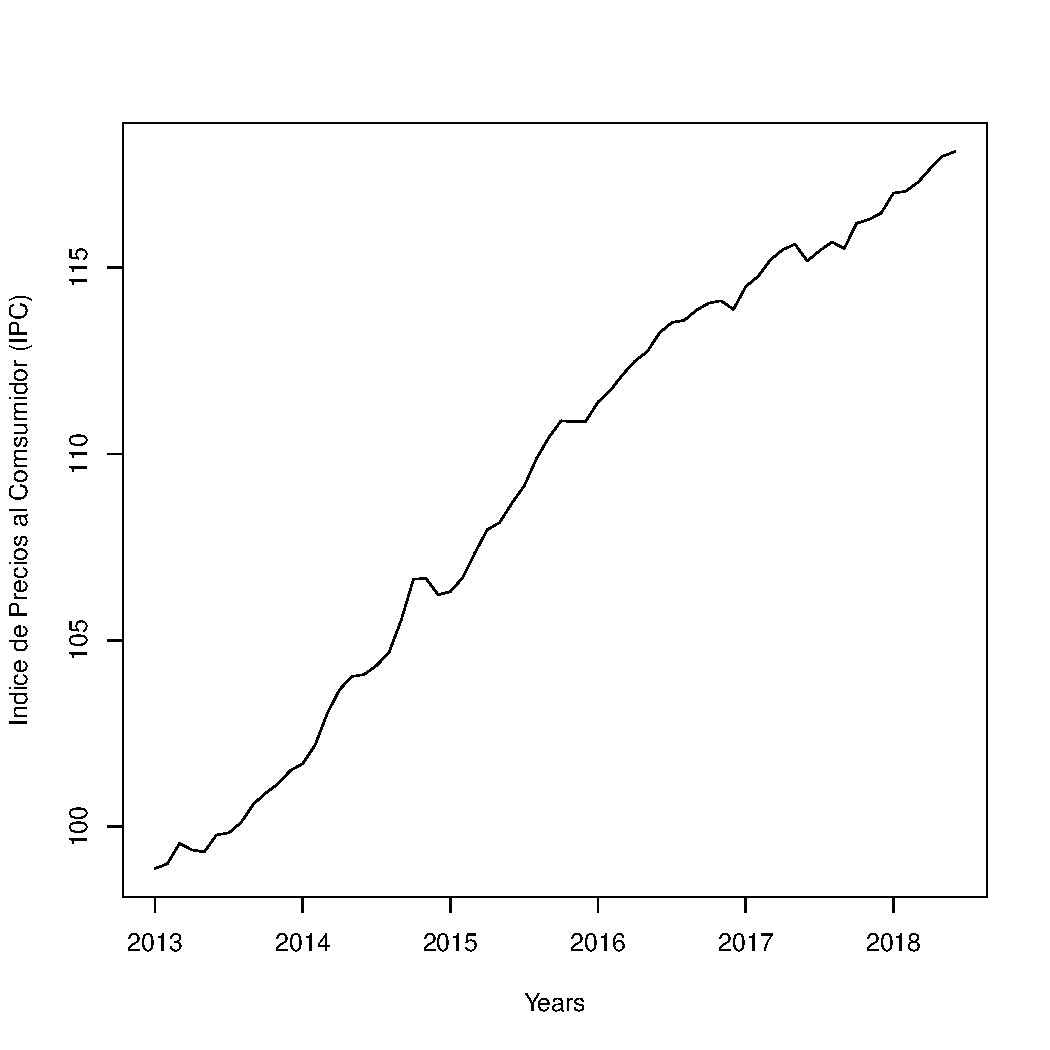
\includegraphics[width=\linewidth]{ipc.pdf}}
	\caption{Serie de tiempo del índice de precios al consumidor (IPC) en Chile.}\label{fig18}
\end{figure}

%\end{frame}

%---------------------------------------------------------
%---------------------Slide 55 --------------------------
%\begin{frame}
%\frametitle{Ejemplo IPC en Chile}
\pagebreak
\subsubsection{Encontrando el orden del modelo. Tendencia, estacionaridad, autocorrelaci\'on.}
%\only<1|handout:1>{
%\begin{exampleblock}{C\'odigo en R}
%
%$\#$ Descomposici\'on\\
%fit $<-$ stl(ipc, s.window=``period")\\
%plot(fit)\\
%
%$\#$ Test de ra\'{\i}z unitaria\\
%adf.test(ipc)\\
%adf.test(diff(ipc))\\
%
%$\#$ Funci\'on de autocorrelaci\'on (AFC) y autocorrelaci\'on parcial (PAFC)\\
%acf(diff(ipc),lag=36,lwd=3)\\
%pacf(diff(ipc),lag=36,lwd=3)\\
%\end{exampleblock}
%}
\lstset{caption=Ejemplo ,framexleftmargin=5mm, frame=shadowbox, rulesepcolor=\color{green}}
\begin{lstlisting}[title={‘Código R: Tendencia, estacionaridad, autocorrelación. ’},basicstyle=\ttfamily]{}
#Descomposicion
fit <- stl(ipc, s.window="period")
plot(fit)
library("tseries")
#TestRaizUnitaria
adf.test(ipc)
adf.test(diff(ipc))
#FuncionAutocorrelacion_yAutocorrelacionParcial
acf(diff(ipc),lag=36,lwd=3)
pacf(diff(ipc),lag=36,lwd=3)
\end{lstlisting}

%\end{frame}
%---------------------------------------------------------
%---------------------Slide 56--------------------------
%\begin{frame}
%\frametitle{Ejemplo IPC en Chile}

%\textbf{Descomposici\'on\ de la serie}\\
\subsection{Descomposici\'on\ de la serie}

\begin{figure}[H]
	\centering
	\textbf{Ejemplo IPC: Descomposición de la serie de IPC}\par\medskip
	\fcolorbox{green}{blue}{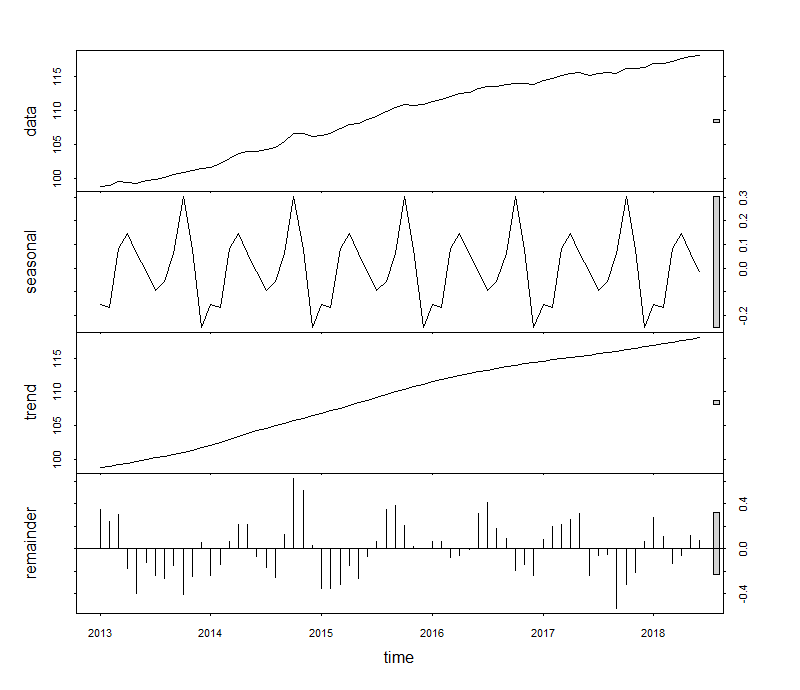
\includegraphics[width=\linewidth]{ipcdecomp.png}}
	\caption{Diferentes componentes de la serie: data: serie original de IPC; seasonal: componente estacional; trend: tendencia de la serie; remainder: componentes irregulares.}\label{fig20}
\end{figure}

%\end{frame}

%---------------------------------------------------------
%---------------------Slide 57--------------------------
%\begin{frame}
%\frametitle{Ejemplo IPC en Chile}

%\textbf{Test de ra\'{\i}z unitaria}\\
%\vspace{4mm}	
%Augmented Dickey-Fuller Test\\
%data:  ipc\\
%Dickey-Fuller = -0.11148, Lag order = 4, p-value =0.99\\
%alternative hypothesis: stationary\\
%\vspace{4mm}	
%Augmented Dickey-Fuller Test\\
%data:  diff(ipc)\\
%Dickey-Fuller = -5.8024, Lag order = 3, p-value = 0.01\\
%alternative hypothesis: stationary\\
\begin{figure}[H]
	\centering
	\textbf{Test de ra\'{\i}z unitaria}\par\medskip
	\fcolorbox{green}{blue}{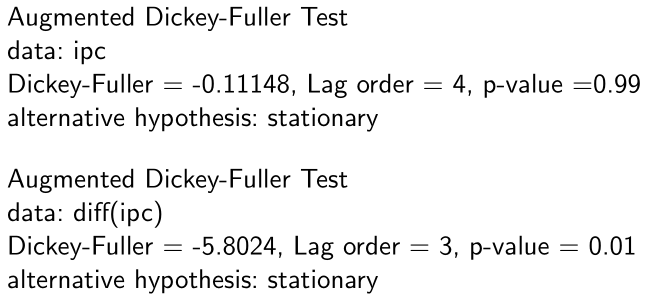
\includegraphics[width=\linewidth]{testRaizUnitIPCChile.png}}
	\caption{Test de Augmented Dickey-Füller sobre data original(ipc) y sobre primera diferencia de la data de ipc(diff(ipc))}\label{fig21}
\end{figure}
%\end{frame}

%---------------------------------------------------------
%---------------------Slide 58--------------------------
%\begin{frame}
%\frametitle{Ejemplo IPC en Chile}
%
%\textbf{Funci\'on de autocorrelaci\'on (AFC) y autocorrelaci\'on parcial (PAFC)}\\
\begin{figure}[H]
	\centering
	\textbf{Funci\'on de autocorrelaci\'on (AFC) y autocorrelaci\'on parcial (PAFC)}\par\medskip
	\fcolorbox{green}{blue}{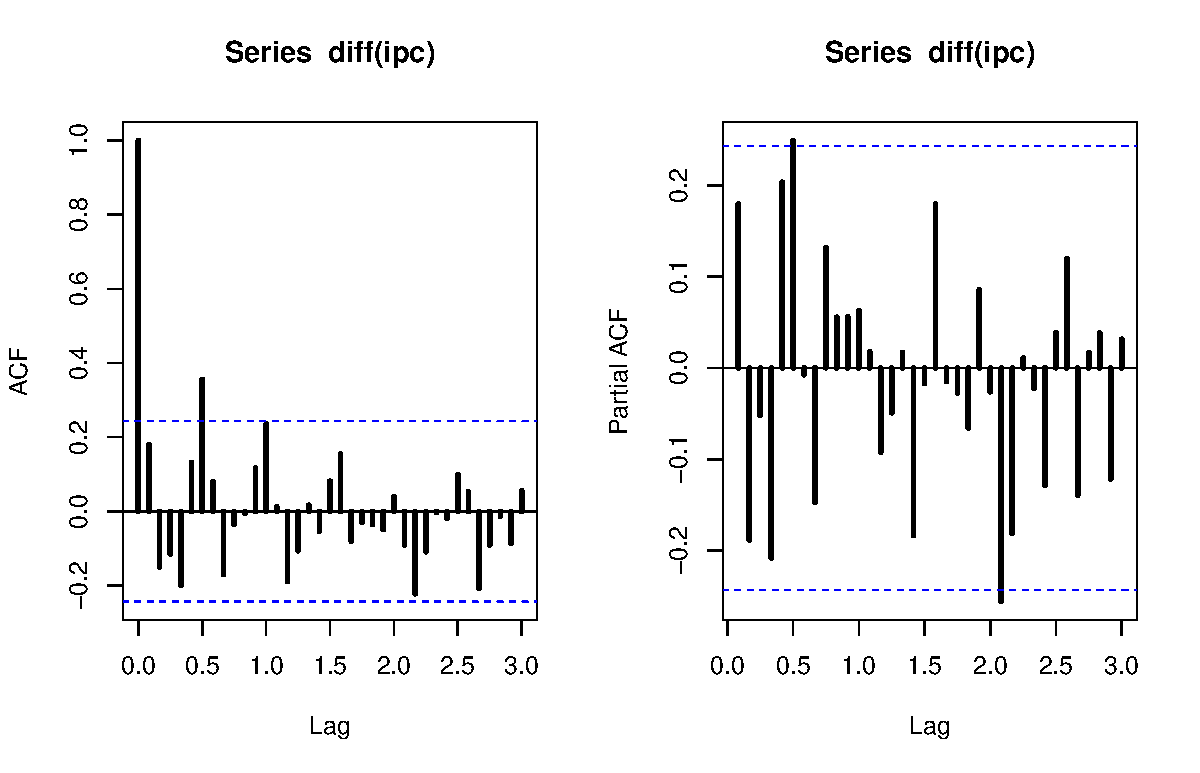
\includegraphics[width=\linewidth]{acfpacdiffipc.pdf}}
	\caption{Izquierda: autocorrelacion de serie de ipc diferenciada. Derecha: autocorrelación parcial de serie de IPC diferenciada.}\label{fig22}
\end{figure}

%\end{frame}

%---------------------------------------------------------
%---------------------Slide 59--------------------------
%\begin{frame}
%\frametitle{Ejemplo IPC en Chile}

%\textbf{Pron\'ostico.}\\
%\vspace{4mm}	
%\only<1|handout:1>{
%\begin{exampleblock}{C\'odigo en R}
%
%train.series =ipc $\left [ 1:44 \right ]$\\
%test.series = ipc $\left [ 45:62 \right ]$\\
%arima.model=arima(train.series, order=c(0,1,1))\\
%forecast=predict(arima.model, length(test.series)\\
%
%mse $<-$sum((forecast$\$$pred-test.series)$\wedge2$)/length(test.series)\\
%mad $<-$ sum(abs(forecast$\$$pred-test.series))/length(test.series)\\
%mape $<-$ sum(abs( 1 - forecast$\$$pred/test.series))/length(test.series)\\
%
%fit $<-$ auto.arima(ipc)\\
%summary(fit)\\
%plot(fit)\\
%mape $<-$ sum(abs(1 - test.series/f$[[``mean"]])$)/length(test.series)\\
%accuracy(fit)\\
%\end{exampleblock}
%}
\lstset{caption=Ejemplo ,framexleftmargin=5mm, frame=shadowbox, rulesepcolor=\color{green}}
\begin{lstlisting}[title={‘Código R: REVISAR: Diapo 59(125)’},basicstyle=\ttfamily]{}
train_series=ipc[1:44]
test_series=ipc[45:62]
arimaModel=arima(train_series, order=c(0,1,1))
forecast=predict(arimaModel, length(test_series))
mse <- sum((forecast$pred-test_series)^2)/length(test_series)
mad <- sum(abs(forecast$pred-test_series))/length(test_series)
mape <- sum(abs(1-test_series/forecast$pred))/length(test_series)
fit <- auto.arima(ipc)
summary(fit)
plot(fit)

mape <- 100*sum(abs(1-test_series/f[["mean"]]))/length(test_series)
accuracy(fit)
\end{lstlisting}

%\end{frame}

%---------------------------------------------------------
%---------------------Slide 60--------------------------
%\begin{frame}
%\frametitle{Ejemplo IPC en Chile}
%\textbf{output ARIMA (0, 1, 1) }\\
%\vspace{4mm}	
%Call:\\
%arima(x = train.series, order = c(0, 1, 1))\\
%
%Coefficients:\\
%\hspace{3em}ma1\\
%\hspace{2.5em}$0.8205$\\
%s.e.\hspace{1em}$ 0.0906$\\
%
%$\sigma^2$ estimated as $0.1029:  log likelihood = -12.68,  aic = 29.37$\\
%\vspace{4mm}
%\textbf{forecast ARIMA (0, 1, 1) }\\
%mse
%[1] 69.80031
%\end{frame}
\begin{figure}[H]
	\centering
	\textbf{Resultado-Parámetros ajuste de modelo ARIMA(0,1,1) y Error de Forecast(MSE)}\par\medskip
	\fcolorbox{green}{blue}{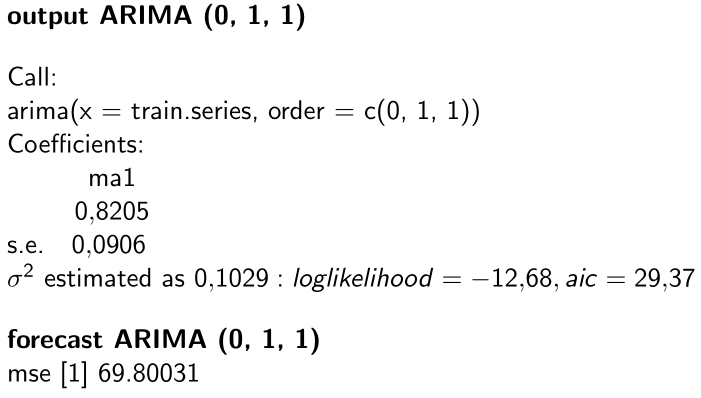
\includegraphics[width=\linewidth]{resultadoArimaD60.png}}
	\caption{Resultados del ajuste del modelo ARIMA(0,1,1) y su error de pronóstico}\label{fig24}
\end{figure}
%---------------------------------------------------------
%---------------------Slide 61--------------------------
%\begin{frame}
%\frametitle{Ejemplo IPC en Chile}
%\textbf{Pron\'ostico - output ARIMA (0, 1, 1) }\\
%\vspace{4mm}	
%$\$$pred\\
%Time Series:\\
%Start = 45 \\
%End = 54 \\
%Frequency = 1 \\
%$\left [ 1 \right ]$ $113.6141$ $113.6253$ $113.6292$ $113.6307$ $113.6311$ $113.6313$\\
%$\left [ 7 \right ]$ $113.6314$ $113.6314$ $113.6314$ $113.6314$\\
%
%$\$$se\\
%Time Series:\\
%Start = 45 \\
%End = 54 \\
%Frequency = 1 \\
%$\left [ 1 \right ]$ $0.3128668$ $0.6841962$ $0.9882296$ $1.2406559$ $1.4565974$\\
%$\left [ 6 \right ]$ $1.6465783$ $1.8174943$ $1.9738906$ $2.1188485$ $2.2545301$\\
%
%\end{frame}
\begin{figure}[H]
	\centering
	\textbf{Pronósticos de modelo ARIMA(0,1,1)}\par\medskip
	\fcolorbox{green}{blue}{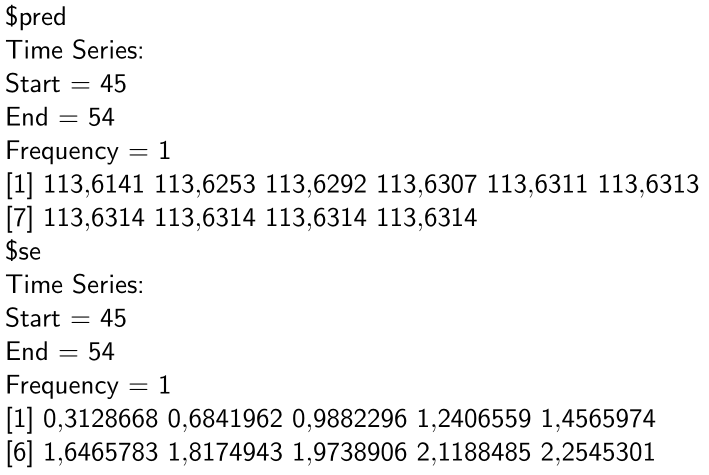
\includegraphics[width=\linewidth]{pronosticoD61.png}}
	\caption{Pronóstico ARIMA(0,1,1)}\label{fig25}
\end{figure}
%---------------------------------------------------------
%---------------------Slide 62--------------------------
%\begin{frame}
%\frametitle{Ejemplo IPC en Chile}
%\textbf{output auto.arima}\\
%
%Series: ipc \\
%ARIMA(0,1,1)(0,0,1)[12] with drift \\
%\vspace{2mm}	
%Coefficients:\\
%\hspace{5em}ma1\hspace{3em}sma1\hspace{3em}drift\\
%\hspace{5em}$0.2329$\hspace{2em}$0.2483$\hspace{2em}$0.2909$\\
%s.e.\hspace{3.5em}$0.1443$\hspace{2em}$0.1396$\hspace{2em}$0.0500$\\
%\vspace{2mm}	
%$\sigma^2$ estimated as $0.07771:  log likelihood=-8.01$\\
%$AIC=24.02$  $ ICc=24.69$  $BIC=32.72$\\
%\vspace{2mm}	
%Training set error measures:\\
%\hspace{7em}ME\hspace{2em}RMSE\hspace{3em}MAE\hspace{2em}MPE\\
%Training set $0.00467571$ $0.2701877$ $0.2012356$ $0.005434612$\\
%\hspace{7em}MAPE\hspace{2em}MASE\hspace{2em}ACF1\\
%Training set $0.185618$ $0.05414794$ $-0.03368001$\\
\begin{figure}[H]
	\centering
	\textbf{Pronósticos de modelo AutoARIMA}\par\medskip
	\fcolorbox{green}{blue}{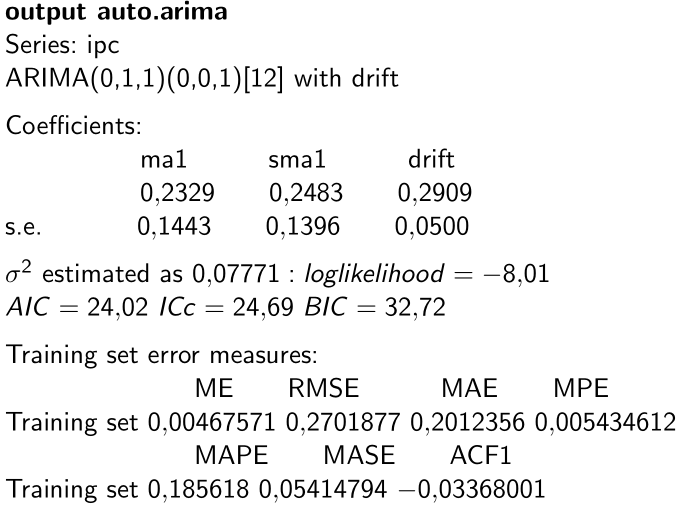
\includegraphics[width=\linewidth]{pronosticoAutoarimaD62.png}}
	\caption{Pronóstico auto ARIMA}\label{fig26}
\end{figure}

%\end{frame}

%---------------------------------------------------------
%---------------------Slide 63--------------------------
%\begin{frame}
%\frametitle{Ejemplo IPC en Chile}
%\textbf{Inverse MA roots  - auto.arima}\\
\vspace{4mm}	
\begin{figure}[H]
	\centering
	\textbf{Inverse MA roots - auto.arima}\par\medskip
	\fcolorbox{green}{blue}{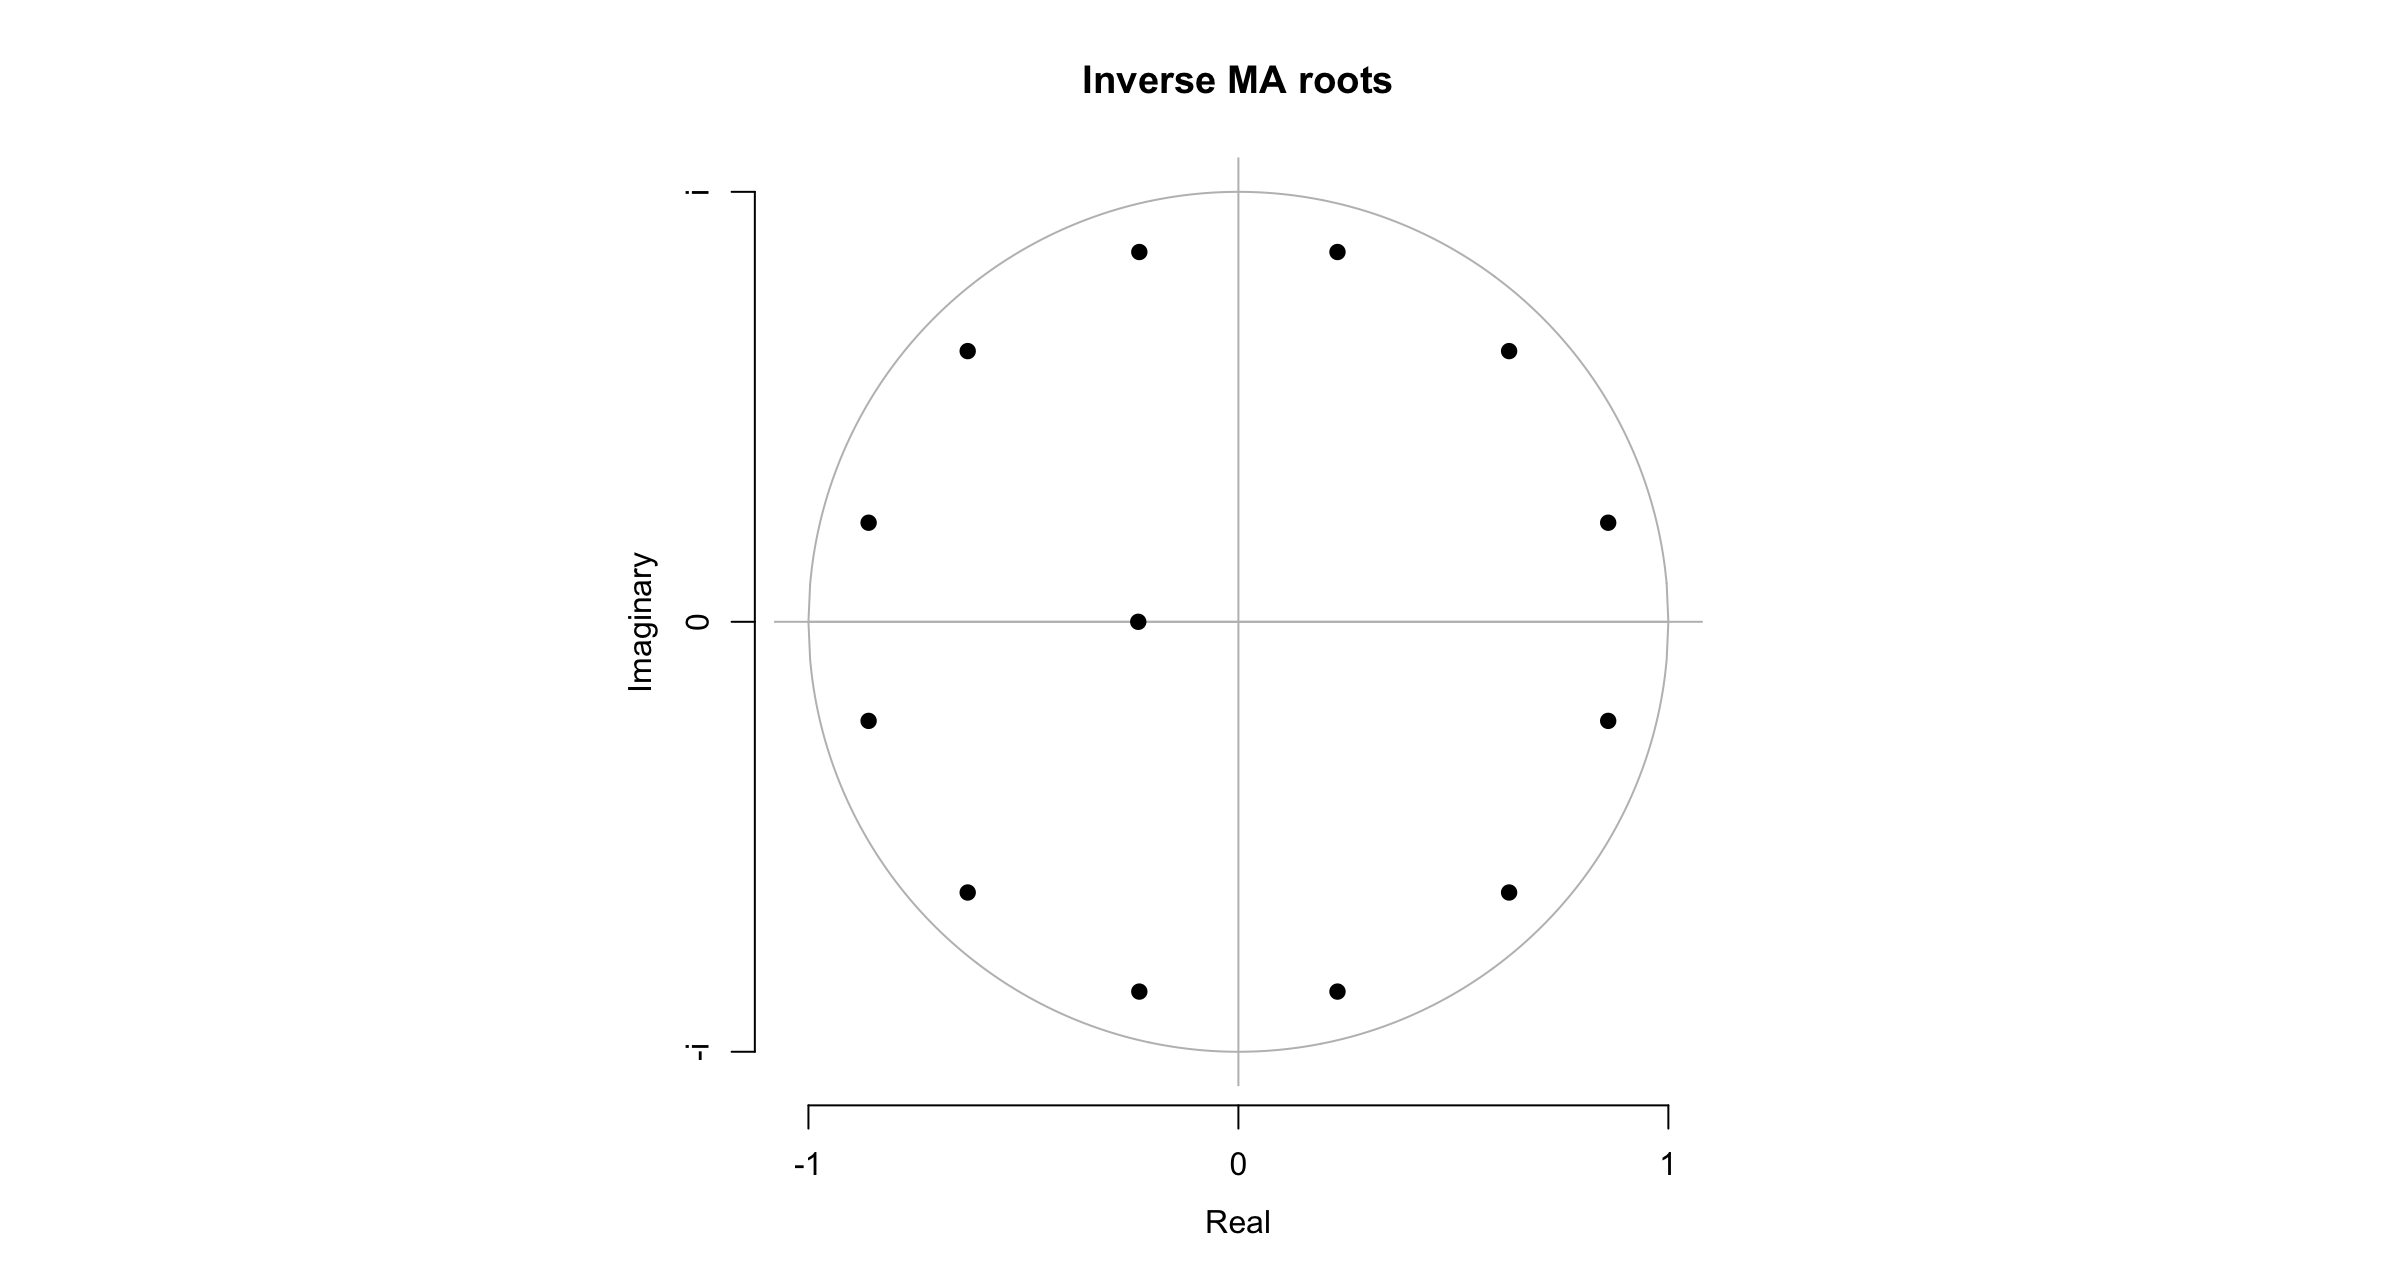
\includegraphics[width=\linewidth]{maroots.png}}
	\caption{Soluciones de ecuación característica - Representación de circulo unitario}\label{fig}
\end{figure}

%\end{frame}

%---------------------------------------------------------
%---------------------Slide 64--------------------------
%\begin{frame}
%\frametitle{Ejemplo IPC en Chile}
%\textbf{Pron\'ostico auto.arima}\\
\vspace{4mm}	
\begin{figure}[H]
	\centering
	\textbf{Forecasts from ARIMA(0,1,1)(0,0,1)[12] with drift}\par\medskip
	\fcolorbox{green}{blue}{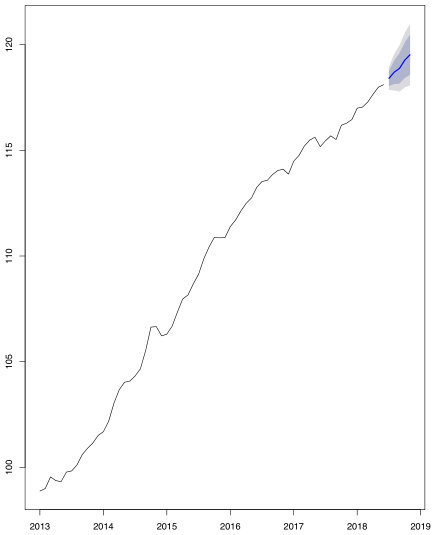
\includegraphics[width=\linewidth]{forecastipc.png}}
	\caption{Ejemplo IPC en Chile: Forecast de modelo auto.arima}\label{fig27}
\end{figure}

%\end{frame}
%\end{section}
%---------------------------------------------------------
%---------------------Slide 65--------------------------
%\begin{section}{Metodolog\'{\i}a de Estimaci\'on de un Modelo ARIMA}
%\begin{frame}
\pagebreak\section{Metodolog\'{\i}a de Estimaci\'on de un Modelo ARIMA}
%\frametitle{Etapas de Estimaci\'on de un Modelo ARIMA}
\subsection{Etapas de Estimaci\'on de un Modelo ARIMA}

%\only<1->{
\begin{itemize}
\item[1] \textbf{Recolecci\'on de datos}: Es recomendable disponer de a lo menos 50 datos, y en el caso de series mensuales, es conveniente trabajar con entre seis y diez a\~nos de datos.
\item[2] \textbf{Representaci\'on gr\'afica de la serie}: Resulta de gran utilidad disponer de diversos gr\'aficos de la serie y sus transfromaciones para decidir sobre la estacionariedad de la misma.
\item[3] \textbf{Transformaci\'on de la serie}: La transformaci\'on de la serie es muchas veces necesaria en caso de encontrarnos con no-estacionaridad.
\item[4] \textbf{Eliminaci\'on de la tendencia}: Al comprobarse gr\'aficamente la existencia de una tendencia, esta debe ser eliminada usando como vimos primeras diferencias, e incluso dos diferencias para una tendencia no lineal.
\item[5] \textbf{Identificaci\'on del modelo}: Se debe determinar el tipo de modelo m\'as adecuado, es decir, el orden de los procesos autorregresivos y de medias m\'oviles de las componentes regular y estacional. Se suelen seleccionar varios modelos alternativos, estimarlos, y contrastarlos, antes de modelar definitivamente la serie.
\item[6] \textbf{Estimaci\'on de los coeficientes del modelo}: A partir del modelo elegido se procede a la estimaci\'on de sus par\'ametros.
\item[7] \textbf{Contraste de validez conjunta del modelo}: Se utilizan los diversos criterios y procedimientos vistos anteriormente para valorar el modelo o modelos seleccionados: test de significancia de par\'ametros, criterios de informaci\'on, covarianzas entre estimadores, coeficiente de correlaci\'on, $R^2$, i.e. suma de cuadrados de errores, etc.
\item[8] \textbf{An\'alisis detallado de los errores}: Los errores extra-muestrales del modelo son determinantes para una valoraci\'on final del modelo. Las diferencias entre valores reales y estimados por el modelo son determinantes para una evaluaci\'on final del modelo.
\item[9] \textbf{Selecci\'on del modelo}: Analizando los resultados de las fases anteriores se decidir\'a sobre el modelo adoptado. Si ninguno de los modelos estudiados nos proporciona resultados suficientemente satisfactorios se vuelve a la etapa 3, revisando todas las decisiones adoptadas.
\item[10] \textbf{Predicci\'on}: Se tomar\'a el modelo v\'alido como f\'ormula inicial de predicci\'on. Ser\'a necesario comparar las predicciones con los valores ya conocidos y, posteriormente, analizar los errores extramuestrales.
\end{itemize}
%}
%
%
%\end{frame}


%---------------------------------------------------------
%---------------------Slide 66--------------------------
%\begin{frame}
%\frametitle{Etapas de Estimaci\'on de un Modelo ARIMA}
%
%\only<1->{
%\begin{itemize}
%\item[5] \textbf{Identificaci\'on del modelo}: Se debe determinar el tipo de modelo m\'as adecuado, es decir, el orden de los procesos autorregresivos y de medias m\'oviles de las componentes regular y estacional. Se suelen seleccionar varios modelos alternativos, estimarlos, y contrastarlos, antes de modelar definitivamente la serie.
%\item[6] \textbf{Estimaci\'on de los coeficientes del modelo}: A partir del modelo elegido se procede a la estimaci\'on de sus par\'ametros.
%\item[7] \textbf{Contraste de validez conjunta del modelo}: Se utilizan los diversos criterios y procedimientos vistos anteriormente para valorar el modelo o modelos seleccionados: test de significancia de par\'ametros, criterios de informaci\'on, covarianzas entre estimadores, coeficiente de correlaci\'on, $R^2$, i.e. suma de cuadrados de errores, etc.
%\end{itemize}
%}

%\end{frame}

%---------------------------------------------------------
%---------------------Slide 67--------------------------
%\begin{frame}
%\frametitle{Etapas de Estimaci\'on de un Modelo ARIMA}
%
%\only<1->{
%\begin{itemize}
%\item[8] \textbf{An\'alisis detallado de los errores}: Los errores extra-muestrales del modelo son determinantes para una valoraci\'on final del modelo. Las diferencias entre valores reales y estimados por el modelo son determinantes para una evaluaci\'on final del modelo.
%\item[9] \textbf{Selecci\'on del modelo}: Analizando los resultados de las fases anteriores se decidir\'a sobre el modelo adoptado. Si ninguno de los modelos estudiados nos proporciona resultados suficientemente satisfactorios se vuelve a la etapa 3, revisando todas las decisiones adoptadas.
%\item[10] \textbf{Predicci\'on}: Se tomar\'a el modelo v\'alido como f\'ormula inicial de predicci\'on. Ser\'a necesario comparar las predicciones con los valores ya conocidos y, posteriormente, analizar los errores extramuestrales.
%\end{itemize}
%}
%
%\end{frame}

%---------------------------------------------------------
%---------------------Slide 68--------------------------
%\begin{frame}
%\frametitle{Resumen de los pasos de Box-Jenkins}
\pagebreak\section{Resumen de los pasos de Box-Jenkins}

\begin{figure}[H]
	\centering
	\textbf{Resumen de los pasos de Box-Jenkins}\par\medskip
	\fcolorbox{green}{blue}{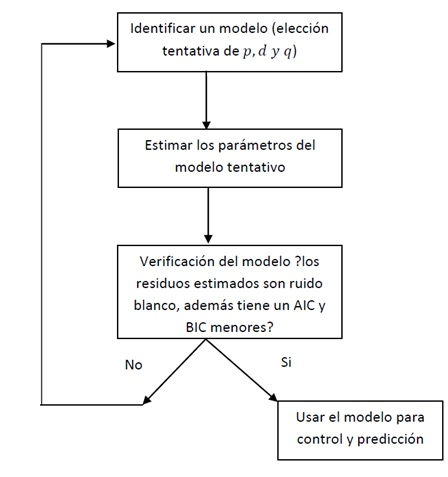
\includegraphics[width=\linewidth]{box_jenkins.png}}
	\caption{Metodología de Box-Jenkins}\label{fig30}
\end{figure}

%\end{frame}
%
%\end{section}

%---------------------------------------------------------
%---------------------Slide 69--------------------------

%\begin{section}{Tarea 2}
%\begin{frame}
%\frametitle{Tarea 2}
\pagebreak\section{Tarea 2}
\begin{mdframed}[style=MyFrame]
Calibrar y evaluar los siguientes modelos para el precio de un commodity (0 activo en \'ultimo caso) a su eleci\'on:\\
\textbf{1.} Camino aleatorio sin drift.,\\
\textbf{2.} Camino aleatorio con drift.\\
\textbf{3.} Promedio de los \'ultimos 5 a\~nos.\\ 
\textbf{4.} Promedio de los \'ultimos 10 a\~nos.\\
\textbf{5.} ARIMA(1,1,0).\\
\textbf{6.} ARIMA(0,1,1).,\\ 
\textbf{7.} ARIMA(1,1,1).,\\ 
\textbf{8.} AR(1).,\\ 
\textbf{9.} AR(2).,\\
\textbf{10.} AR(3).\\
\textbf{11.} $\alpha$ constante, $\psi$ = 1 y $\delta$ sigue un camino aleatorio.\\
\textbf{12.} $\psi$=1,$\delta$=0 y ?sigue un camino aleatorio.\\
\textbf{13.} $\alpha$ constante, $\delta$ y $\psi$ siguen caminos aleatorios con innovaciones independientes.\\
\textbf{14.} $\delta$ = 0, $\alpha$ y $\psi$ siguen caminos aleatorios con innovaciones independientes.\\ 
\textbf{15.} $\alpha$ constante, $\delta$ = 0 y $\psi$ sigue un camino aleatorio.\\
\textbf{16.} $\alpha$, $\delta$ y $\psi$ siguen caminos aleatorios con innovaciones independientes.\\
\textbf{17.} $\alpha$ constante, $\delta$ = 0 y $\psi$ sigue un AR(1).\\
\textbf{18.} $\alpha$ y $\delta$ constantes, $\psi$ sigue un AR(1).\\
\vspace{4mm}	
Basarse en paper anexo.
\end{mdframed}
%\end{frame}
%\end{section}






\curinstructor{Marcelo Villena Chamorro PhD.}
\chapter{Tópico III.- Vector Autoregressive Models}

%---------------------Slide 3--------------------------
%\begin{section}{Introducci\'on}
%	\begin{frame}
%		\frametitle{Vector Autoregressive Models}
\section{Vector Autoregressive Models}
\subsection{Introducci\'on}
		Desde la cr\'{\i}tica de Sims \cite{sims1980macroeconomics} a principios de los años ochenta del siglo pasado, el an\'alisis multivariado de datos, en el contexto de los modelos autorregresivos vectoriales (en adelante, VAR por su sigla en ingl\'es  \textbf{Vector Autoregressive Models}) se ha transformado en un instrumento est\'andar en econometr\'{\i}a. \\
		Debido a que las pruebas estad\'{\i}sticas se utilizan con frecuencia para determinar interdependencias y relaciones din\'amicas entre variables, esta metodolog\'{\i}a pronto se enriqueci\'o al incorporar información antes no considerada.\\	
%	\end{frame}
	%---------------------------------------------------------
	%---------------------Slide 4--------------------------
%	\begin{frame}
%		\frametitle{Vector Autoregressive Models}	
		Los modelos VAR explican las variables end\'ogenas \'unicamente por su propia historia, adem\'as de los regresores determin\'{\i}sticos. En contraste, los modelos VAR estructurales (en adelante, SVAR, por Structural VAR) permiten el modelado expl\'{\i}cito de la interdependencia contempor\'anea entre las variables del lado izquierdo. Por lo tanto, este tipo de modelos intenta eludir las deficiencias de los modelos VAR.\\
%	\end{frame}
	%---------------------------------------------------------
	%---------------------Slide 5--------------------------
%	\begin{frame}
%		\frametitle{Vector Autoregressive Models}
		Un VAR es un sistema de dos o m\'as series de tiempo que se modela considerando rezagos de las variables y la interacción din\'amica que pudiera existir entre ellas. Consiste fundamentalmente de dos dimensiones, el n\'umero de variables (g) y el n\'umero de rezagos (k). El caso más simple es un VAR bivariado:
		
		\begin{equation*}
		y_{1t} = \beta_{10} + \beta_{11} y_{1t-1} + \dots{} +  \beta_{1k} y_{1t-k} + \alpha_{11} y_{2t-1} + \dots{} +  \alpha_{1k} y_{2t-k} + \mu_1t
		\end{equation*}
		\begin{equation*}
		y_{2t} = \beta_{20} + \beta_{21} y_{2t-1} + \dots{} +  \beta_{2k} y_{2t-k} + \alpha_{21} y_{1t-1} + \dots{} +  \alpha_{2k} y_{1t-k} + \mu_2t
		\end{equation*}
		
		donde $u_{it}$ es un t\'ermino de error con $E(u_{it})=0$, $i =1,2$; $E(u_{1t} u_{2t})=0$. El supuesto de independencia de los errores puede relajarse como veremos m\'as adelante.
		
		El an\'alisis podr\'{\i}a extenderse por ejemplo a un modelo VAR (g), donde tenemos g variables y g ecuaciones.
		
%	\end{frame}
%\end{section}
%---------------------------------------------------------
%---------------------Slide 6--------------------------
%\begin{section}{Notaci\'on y Conceptos}
%	\begin{frame}
%		\frametitle{Vector Autoregressive Models}
\pagebreak\subsection{Notaci\'on y Conceptos}
		Una caracter\'{\i}stica importante de los modelos VAR es la sencillez de su notaci\'on. Por ejemplo, considere el caso de arriba, donde k = 1. Podemos escribir este modelo como:
		\begin{equation*}
		y_{1t} = \beta_{10} + \beta_{11} y_{1t-1} + \alpha_{11} y_{2t-1} + \mu_1t
		\end{equation*}
		\begin{equation*}
		y_{2t} = \beta_{20} + \beta_{21} y_{2t-1} + \alpha_{21} y_{1t-1} + \mu_2t
		\end{equation*}
		
		\'o
		
		\begin{gather}
		\begin{pmatrix} y_{1t} \\ y_{2t} \end{pmatrix}
		=
		\begin{pmatrix} \beta_{10} \\ \beta_{20} \end{pmatrix}
		+
		\begin{pmatrix} \beta_{11} & \alpha_{11} \\ \alpha_{21} & \beta{21} \end{pmatrix}
		\begin{pmatrix} y_{1t-1} \\ y_{2t-1} \end{pmatrix}
		+
		\begin{pmatrix} \mu_{1t} \\ \mu_{2t} \end{pmatrix}
		\end{gather}
		
		o incluso de forma m\'as compacta como
		
		\begin{gather}
		\begin{matrix} y_{t} =       \\ g x 1 \end{matrix}
		\begin{matrix} \beta_{0} +\\ g x 1 \end{matrix}
		\begin{matrix} \beta_{1}   \\ g x g \end{matrix}
		\begin{matrix} y_{t-1} +    \\ g x 1 \end{matrix}
		\begin{matrix} \mu_{1t}    \\ g x 1 \end{matrix}
		\end{gather}
		
%	\end{frame}
	%---------------------------------------------------------
	%---------------------Slide 7--------------------------
%	\begin{frame}
%		\frametitle{Vector Autoregressive Models}
		Este modelo se puede extender al caso en que hay $k$ retardos de cada variable en cada ecuaci\'on:
		
		\begin{gather}
		\begin{matrix} y_{t} =       \\ g x 1 \end{matrix}
		\begin{matrix} \beta_{0} +\\ g x 1 \end{matrix}
		\begin{matrix} \beta_{1}   \\ g x g \end{matrix}
		\begin{matrix} y_{t-1} +    \\ g x 1 \end{matrix}
		\begin{matrix} \beta_{2}   \\ g x g \end{matrix}
		\begin{matrix} y_{t-2} +    \\ g x 1 \end{matrix}
		\begin{matrix} \dots{}    \\  \end{matrix}
		\begin{matrix} \beta_{k}   \\ g x g \end{matrix}
		\begin{matrix} y_{t-k} +    \\ g x 1 \end{matrix}
		\begin{matrix} \mu_{1t}    \\ g x 1 \end{matrix}
		\end{gather}
		
		Tambi\'en podemos extender este al caso en que el modelo incluye t\'erminos de primera diferencia y relaciones de cointegraci\'on (un VECM que veremos m\'as adelante).
		
%	\end{frame}
%\end{section}
%---------------------------------------------------------
%---------------------Slide 8--------------------------
%\begin{section}{VAR versus Modelos Estructurales}
%	\begin{frame}
%		\frametitle{Vector Autoregressive Models}
\subsection{VAR versus Modelos Estructurales}
		
		\textbf{Vector Autoregressive Models Compared with Structural Equations Models}\\
		
		\textbf{Ventajas del modelo VAR:}
%		\only<1->{
			\begin{itemize}
				\item No es necesario especificar qu\'e variables son end\'ogenas o ex\'ogenas - todas son end\'ogenas.
				\item Permite que el valor de una variable dependa de algo m\'as que sus propios rezagos o combinaciones de t\'erminos de ruido blanco, por lo que son m\'as generales que nuestro ya conocido modelo ARIMA.
				\item Siempre que no tengamos t\'erminos contempor\'aneos sobre el lado derecho de las ecuaciones, podremos utilizar OLS por separado en cada ecuaci\'on 
				\item Los pron\'osticos son a menudo mejores que los modelos ``estructurales tradicionales".
			\end{itemize}
%		}
		
%	\end{frame}
	%---------------------------------------------------------
	%---------------------Slide 9--------------------------
%	\begin{frame}
%		\frametitle{Vector Autoregressive Models}
		
%		\textbf{Vector Autoregressive Models Compared with Structural Equations Models}\\
		
		\textbf{Problemas con el VAR:}
%		\only<1->{
			\begin{itemize}
				\item Los modelos VAR son ate\'oricos (al igual que los modelos ARIMA).
				\item ?`C\'omo se decide la longitud del rezago apropiado?
				\item Son tantos parámetros! Si tenemos g ecuaciones para las g variables y tenemos k rezagos de cada una de las variables en cada ecuaci\'on, tenemos que estimar (g+ kg2) parámetros. Por ejemplo si g = 3, y k = 3, tendremos 30 par\'ametros!!!
				\item ?`Tenemos que asegurar que todos los componentes del modelo VAR sean estacionarios?
				\item ?`C\'omo interpretar los coeficientes?
			\end{itemize}
%		}
		
%	\end{frame}
%\end{section}
%---------------------------------------------------------
%---------------------Slide 10--------------------------
%\begin{section}{La elecci\'on de la longitud del rezago \'optimo para un VAR}
%	\begin{frame}
%		\frametitle{Vector Autoregressive Models}
\subsection{La elecci\'on de la longitud del rezago \'optimo para un VAR}
		
		Existen dos enfoques posibles:\begin{itemize}
			\item i) restricciones de ecuaciones cruzadas,
			\item ii) los criterios de informaci\'on
		\end{itemize}
		
		\textbf{Restricciones de ecuaciones cruzadas}\\
		En el esp\'{\i}ritu de un modelado VAR (sin restricciones), cada ecuaci\'on debe tener la misma longitud de rezago\\
		Supongamos que un VAR bivariado(8) se estim\'o utilizando datos trimestrales con 8 rezagos para las dos variables en cada ecuaci\'on, y queremos examinar la restricci\'on de que los coeficientes de los rezagos 5 a 8 son conjuntamente cero. Esto se puede hacer utilizando una prueba de raz\'on de verosimilitud.\\
		
%	\end{frame}
	%---------------------------------------------------------
%---------------------Slide 11--------------------------
%\begin{frame}
%	\frametitle{Vector Autoregressive Models}
%	\textbf{La elecci\'on de la longitud del rezago \'optimo para un VAR}
	Denotamos la matriz de varianza-covarianza de los residuales (dada por $\hat{\mu}\hat{\mu}' /T$), como $\hat{\sum}$. La prueba de raz\'on de verosimilitud de esta hip\'otesis conjunta está dada por:
	
	\begin{equation*}
	LR = T\left [ log |\hat{\sum_r}| - log |\hat{\sum_u}| \right ]
	\end{equation*}
	
	donde $\hat{\sum_r}$ es la matriz de varianza-covarianza de los residuos para el modelo restringido (con 4 rezagos), $\hat{\sum_u}$ es la matriz de varianza-covarianza de los residuos para el modelo VAR sin restricciones (con 8 rezagos), y T es el tama\~no de la muestra.\\
	El estad\'{\i}stico de prueba se distribuye asint\'oticamente como una $\chi^2$ con grados de libertad igual al n\'umero total de restricciones. 
	
%\end{frame}
%---------------------------------------------------------
%---------------------Slide 12--------------------------
%\begin{frame}
%	\frametitle{Vector Autoregressive Models}
%	\textbf{La elecci\'on de la longitud del rezago \'optimo para un VAR}
	
	En el caso del VAR anterior, estamos restringiendo 4 rezagos de dos variables en cada una de las dos ecuaciones, un total de 4 * 2 * 2 = 16 restricciones.\\
	En el caso general en el que tenemos un VAR con p ecuaciones, y queremos imponer la restricci\'on de que los \'ultimos q rezagos tienen coeficientes cero,  habría un total de p2q restricciones.\\
	\textit{Desventajas: La realizaci\'on de la prueba LR es complicada y requiere una supuesto de normalidad de las perturbaciones.}
	
%\end{frame}
%---------------------------------------------------------
%---------------------Slide 13--------------------------
%\begin{frame}
%	\frametitle{Vector Autoregressive Models}
	
	\textbf{Criterios de informaci\'on para la Selecci\'on de Lags del VAR}
	
	Se requieren versiones multivariadas de los criterios de informaci\'on. Estos pueden definirse como:\\
	Akaike information criterion
	\begin{equation*}
	MAIC = ln |\sum| + 2k'/T 
	\end{equation*}
	Bayesian or Schwarz criterion
	\begin{equation*}
	MSBIC = ln |\sum| + k'/T ln(T) 
	\end{equation*}
	
	\begin{equation*}
	MHQIC = ln |\sum| + 2k/T ln(ln(T))
	\end{equation*}
	
	donde toda la notaci\'on se mantiene y $k'$ es el n\'umero total de regresores en todas las ecuaciones, que ser\'a igual a g2k + g para las g ecuaciones, cada una con k retardos para las g variables, m\'as un t\'ermino constante en cada ecuaci\'on. Los valores de los criterios de informaci\'on se construyen para 0, 1, $\dots{}$ retardos (hasta alg\'un m\'aximo pre-especificado de $\bar{k}$).
	
%\end{frame}
%---------------------------------------------------------
%---------------------Slide 14--------------------------
%\begin{frame}
%	\frametitle{Vector Autoregressive Models}
%	\textbf{Ejemplo Modelo VAR}
\textbf{Ejemplo Modelo VAR}
	\cite{lutkepohl2004applied} utilizaron las siguientes series: productividad laboral (prod) definida como la diferencia logar\'{i}tmica entre el PIB y el empleo, el logaritmo del empleo (e), la tasa de desempleo (U) y los salarios reales (rw), definidos como el logaritmo del \'{i}ndice del salario real. Los datos provienen de la base de datos de la OCDE y abarcan desde el primer trimestre de 1980 hasta el cuarto trimestre de 2004.
	
%	\only<1|handout:1>{
%		\begin{exampleblock}{C\'odigo en R}
%			
%			rm(list=ls())\\
%			install.packages(``vars")\\
%			library(``vars")\\
%			data(``Canada")\\
%			summary(Canada)\\
%			plot(Canada, nc = 2, xlab = ``")\\
%			adf2 $<-$ summary(ur.df(Canada[, ``prod"], type = ``drift", lags = 1))
%			
%		\end{exampleblock}
%	}
\lstset{caption=Ejemplo Modelo VAR: \textquotedblleft Canadian labor market\textquotedblright,framexleftmargin=5mm, frame=shadowbox, rulesepcolor=\color{green}}
\begin{lstlisting}[title={‘Código R: ejemplo Modelo VAR},basicstyle=\ttfamily]{}\label{ejemploModeloVAR}
rm(list=ls())
install.packages(vars)
library(vars)
data("Canada")
summary(Canada)
plot(Canada, nc = 2, xlab = "")
adf2 <- summary(ur.df(Canada[, "prod"],type="drift",lags=1))
\end{lstlisting}
	
%\end{frame}

%---------------------------------------------------------
%---------------------Slide 15--------------------------
%\begin{frame}
%	\frametitle{Vector Autoregressive Models}
%	\textbf{Ejemplo Modelo VAR}
	
	
	\begin{figure}[H]
		\centering
		\textbf{Ejemplo Modelo VAR: Gráficos de las series de tiempo de cada variable}\par\medskip
		\fcolorbox{green}{blue}{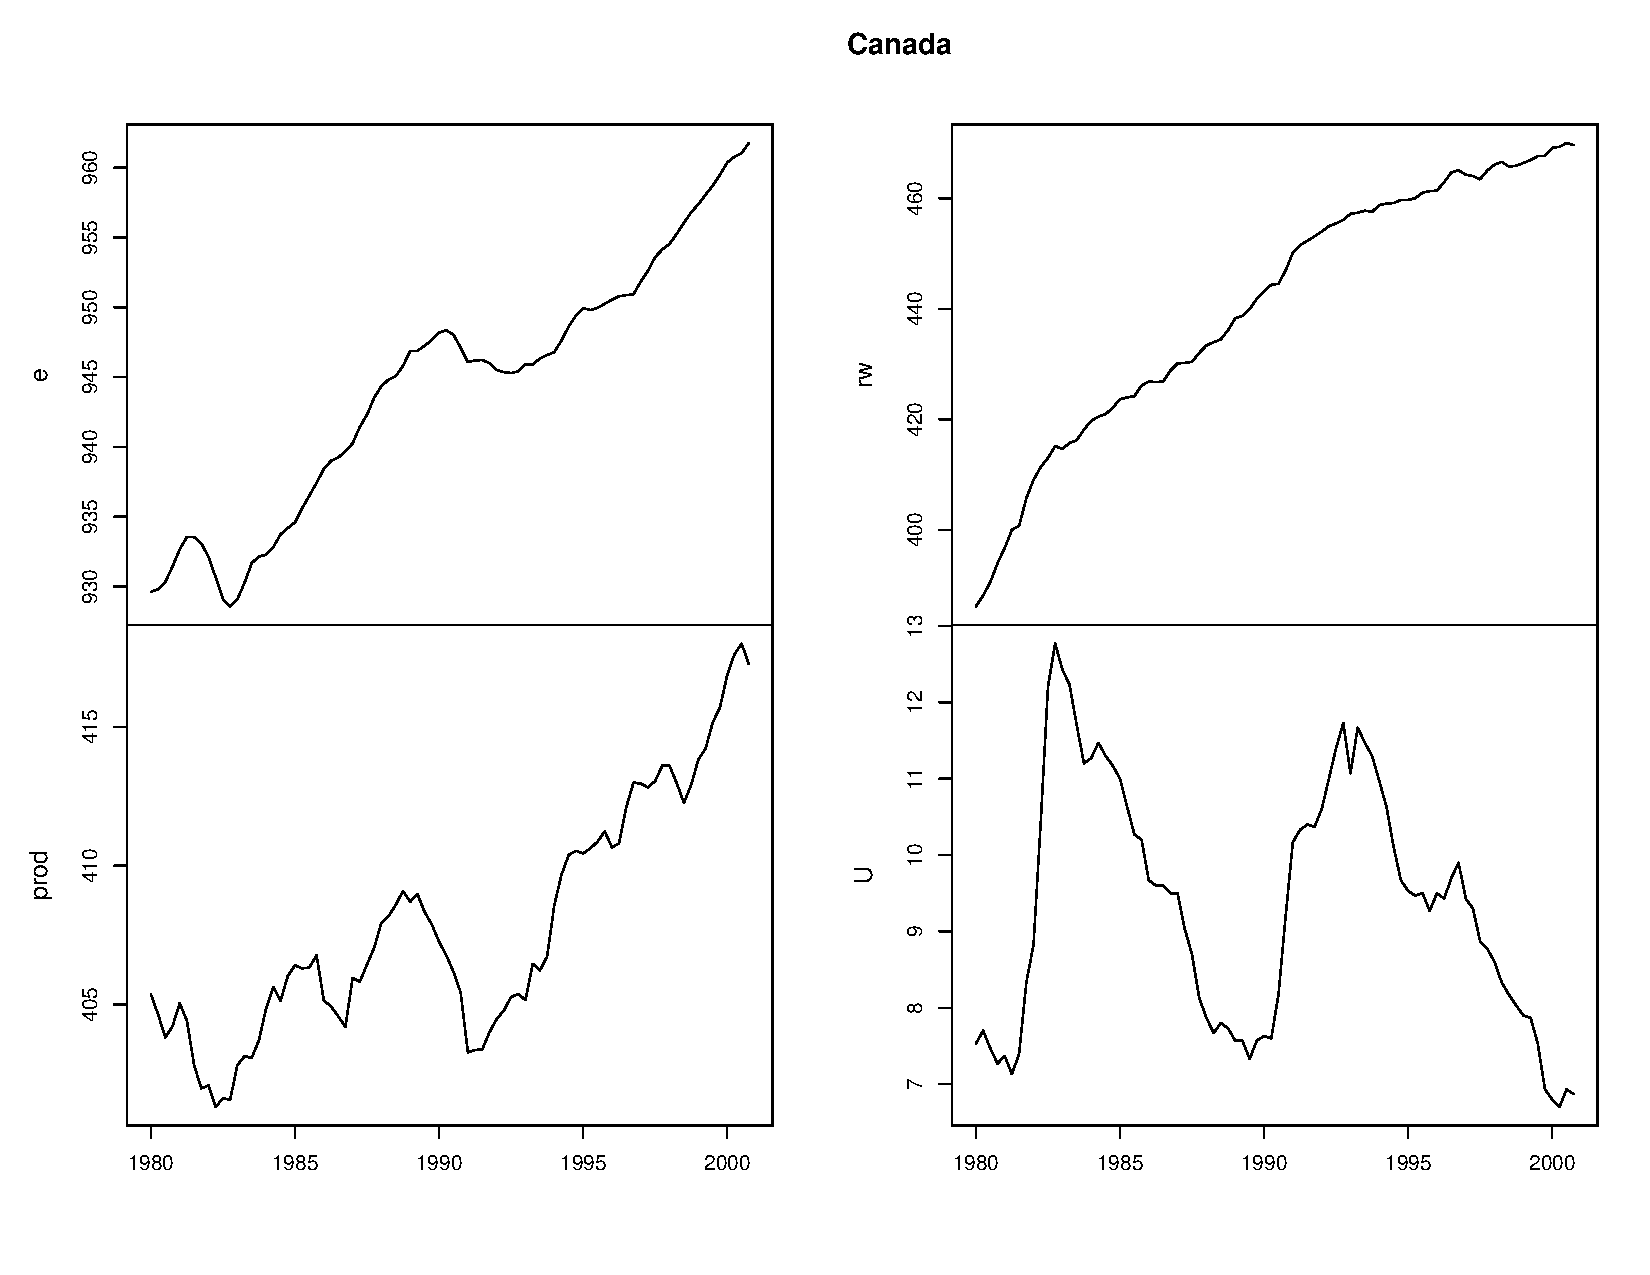
\includegraphics[width=\linewidth,scale=0.5]{canada.pdf}}
		\caption{e: logaritmo del empleo, prod: productividad definida como la log diferencia entre GDP y empleo,rw: salarios reales , U: tasa de desempleo.}\label{figd15}
%		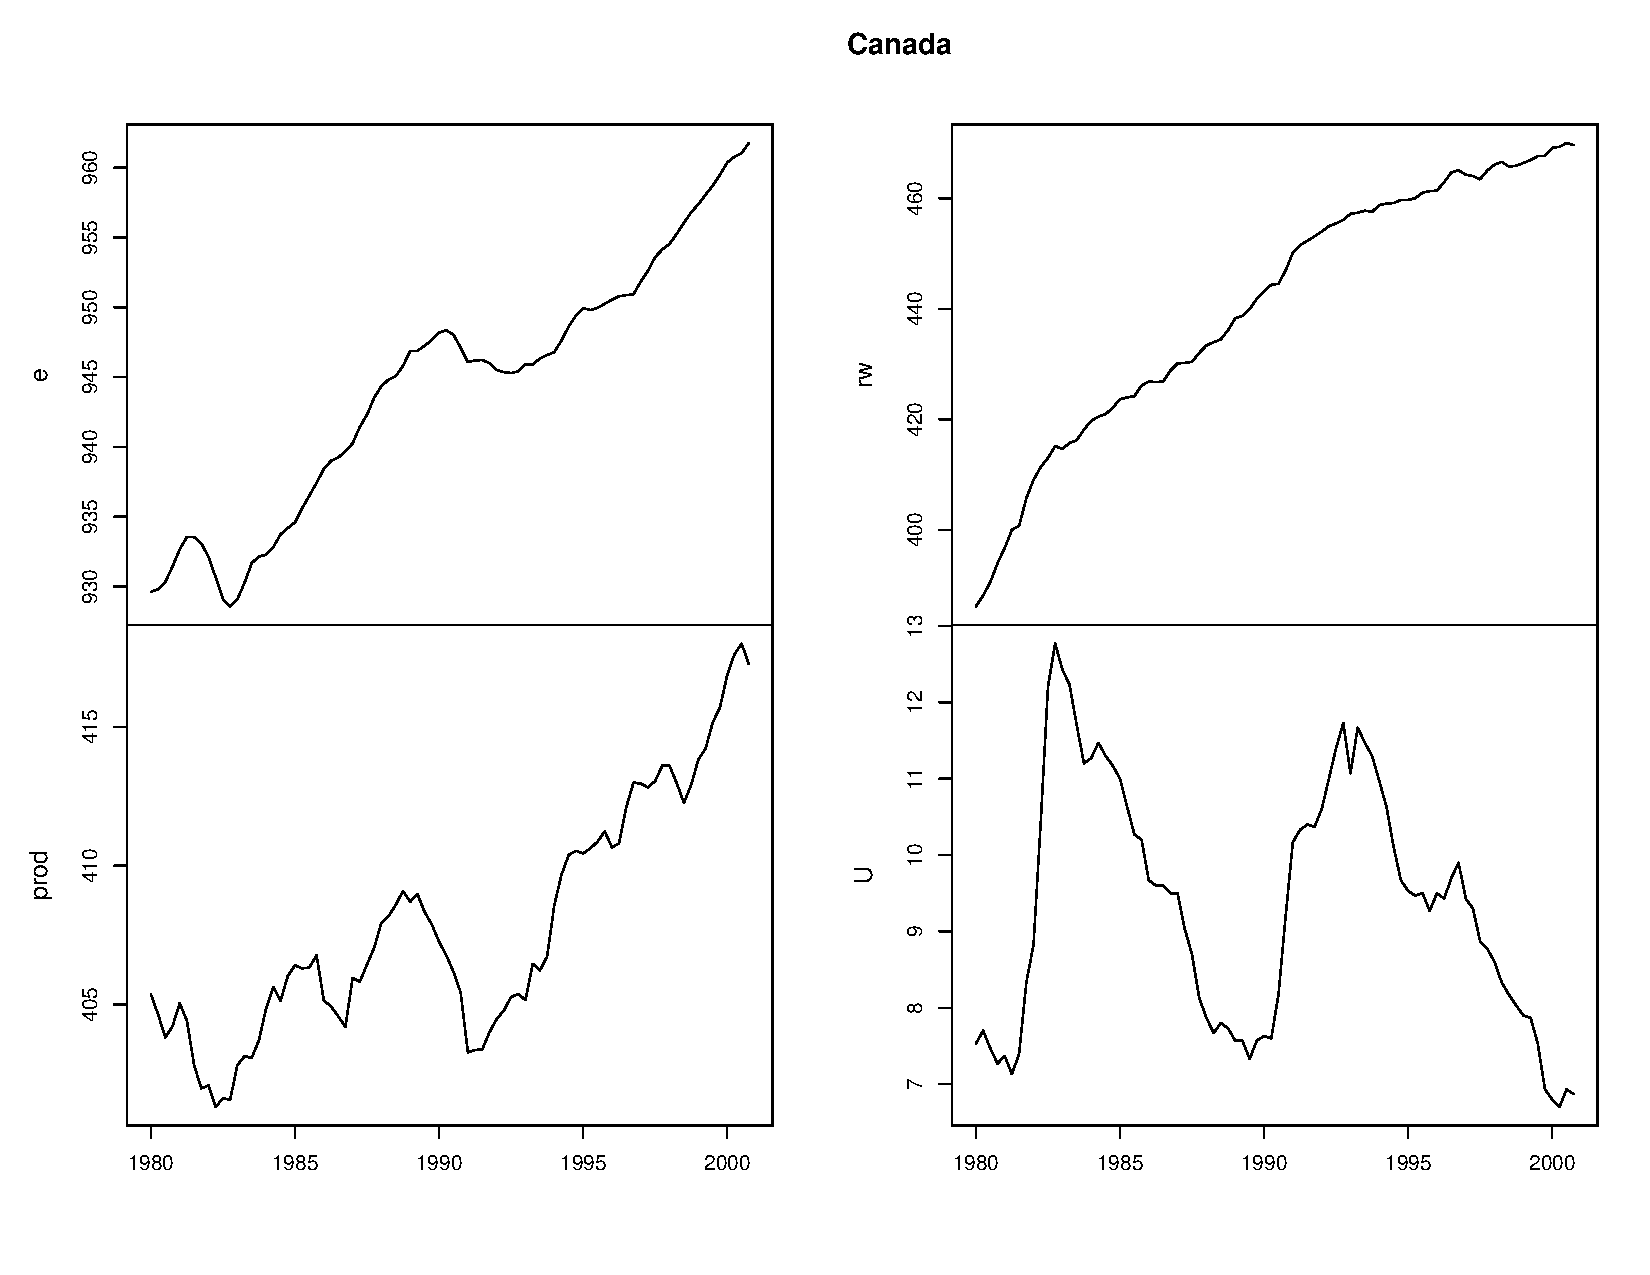
\includegraphics[scale=0.35]{canada.pdf}
	\end{figure}
	
%\end{frame}
%---------------------------------------------------------
%---------------------Slide 16--------------------------
%\begin{frame}
%	\frametitle{Vector Autoregressive Models}
%	\textbf{Ejemplo Modelo VAR}
	
	
	\begin{figure}[H]
		\centering
		\textbf{Modelo VAR: resumen de variables}\par\medskip
		\fcolorbox{green}{blue}{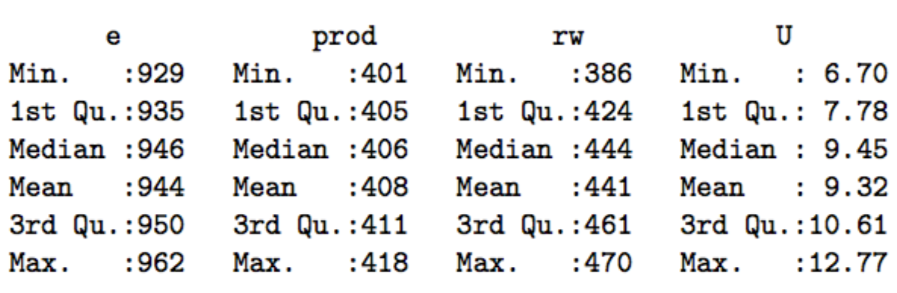
\includegraphics[width=\linewidth,scale=0.5]{summ.png}}
		\caption{Estadística resumen para variables del modelo VAR.}\label{figd16}
%		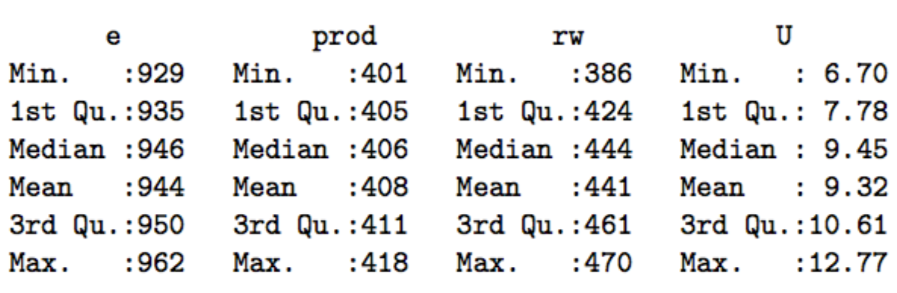
\includegraphics[scale=0.5]{summ.pdf}
	\end{figure}
	
%\end{frame}

%---------------------------------------------------------
%---------------------Slide 17--------------------------
%\begin{frame}
%	\frametitle{Vector Autoregressive Models}
%	\textbf{Ejemplo Modelo VAR}
	\begin{figure}[H]
		\centering
		\textbf{Ejemplo VAR: Augmented DF Test Unit Root Test}\par\medskip
		\fcolorbox{green}{blue}{\includegraphics[scale=0.5]{df.png}}
		\caption{Test de Dickey-Füller Aumentado para evaluar la presencia de raiz unitaria en la serie  \textquotedblleft prod \textquotedblright. El modelo es considerado con \textquotedblleft drift \textquotedblright y un rezago(lags=1).}\label{figd17}
%		\includegraphics[scale=0.32]{df.pdf}
	\end{figure}
	
%\end{frame}

%---------------------------------------------------------
%---------------------Slide 18--------------------------
%\begin{frame}
%	\frametitle{Vector Autoregressive Models}
%	\textbf{Ejemplo Modelo VAR}
%	
%	\only<1|handout:1>{
%		\begin{exampleblock}{C\'odigo en R}
%			
%			VARselect(Canada, lag.max = 8, type = ``both")\\
%			Canada $<-$ Canada[, c(``prod", ``e", ``U", ``rw")]\\
%			p1ct $<-$ VAR(Canada, p = 1, type = ``both")\\
%			p1ct\\
%			\\
%			summary(p1ct, equation = ``e")\\
%			plot(p1ct, names = ``e")\\
%			\\
%			ser11 $<-$ serial.test(p1ct, lags.pt = 16, type = ``PT.asymptotic")\\
%			ser11$serial\\
%			\\
%			norm1 $<-$ normality.test(p1ct)\\
%			norm1$\$$jb.mul\\
%			\\
%			prd $<-$ predict(plct, n.ahead = 10, ci = 0.95, dumvar = NULL)\\
%			print(prd)\\
%			plot(prd, ``single")
%			
%		\end{exampleblock}
%	}
%	
%\end{frame}
\pagebreak
\lstset{caption=Ejemplo Modelo VAR2,framexleftmargin=5mm, frame=shadowbox, rulesepcolor=\color{green}}
\begin{lstlisting}[title={‘Código R: ejemplo Modelo VAR Mercado laboral canadiense},basicstyle=\ttfamily]{}
VARselect(Canada,lag.max = 8,type = "both")
Canada<Canada[, c("prod", "e", "U", "rw")]

p1ct<-VAR(Canada, p = 1, type = "both")
p1ct
summary(p1ct, equation = "e")
plot(p1ct, names = "e")

ser11<-serial.test(p1ct, lags.pt = 16, type = "PT.asymptotic")
ser11$serial
norm1<-normality.test(p1ct)
norm1$jb.mul
prd<-predict(p1ct, n.ahead = 10, ci = 0.95, dumvar = NULL)
print(prd)
plot(prd, "single")

\end{lstlisting}

%---------------------------------------------------------
%---------------------Slide 19--------------------------
%\begin{frame}
%	\frametitle{Vector Autoregressive Models}
%	\textbf{Ejemplo Modelo VAR - instrucci\'on VARselect}
	
	\begin{figure}[H]
		\centering
		\textbf{Ejemplo Modelo VAR: selección de modelos: instrucci\'on VARselect}\par\medskip
		\fcolorbox{green}{blue}{\includegraphics[scale=0.4]{selection.png}}
		\caption{Cada uno de los modelos contiene mediciones de AIC, HQ, SC y FPE}\label{fig34}
%		\includegraphics[scale=0.4]{selection.pdf}
	\end{figure}
	
%\end{frame}

%---------------------------------------------------------

%---------------------Slide 20--------------------------
%\begin{frame}
%	\frametitle{Vector Autoregressive Models}
%	\textbf{Ejemplo Modelo VAR - instrucci\'on VAR}
	
	\begin{figure}[H]
		\centering
		\textbf{Ejemplo Modelo VAR: instrucción VAR}\par\medskip
		\fcolorbox{green}{blue}{\includegraphics[width=\linewidth,scale=0.5]{var1.png}}
		\caption{Coeficientes de la ecuación pea variable \textquotedblleft prod \textquotedblright.}\label{fig35}
%		\includegraphics[scale=0.4]{var1.pdf}
	\end{figure}
	
		\begin{figure}[H]
		\centering
		\textbf{Ejemplo Modelo VAR: instrucción VAR}\par\medskip
		\fcolorbox{green}{blue}{\includegraphics[width=\linewidth,scale=0.4]{var2.png}}
		\caption{Coeficientes de la ecuación pea variable \textquotedblleft rw \textquotedblright.}\label{fig36}
		%		\includegraphics[scale=0.4]{var1.pdf}
	\end{figure}
		\begin{figure}[H]
		\centering
		\textbf{Ejemplo Modelo VAR: instrucción VAR}\par\medskip
		\fcolorbox{green}{blue}{\includegraphics[width=\linewidth,scale=0.4]{var3.png}}
		\caption{Coeficientes de la ecuación pea variable \textquotedblleft U \textquotedblright.}\label{fig37}
		%		\includegraphics[scale=0.4]{var1.pdf}
	\end{figure}
		\begin{figure}[H]
		\centering
		\textbf{Ejemplo Modelo VAR: instrucción VAR}\par\medskip
		\fcolorbox{green}{blue}{\includegraphics[width=\linewidth,scale=0.4]{var4.png}}
		\caption{Coeficientes de la ecuación para variable \textquotedblleft e \textquotedblright.}\label{fig38}
		%		\includegraphics[scale=0.4]{var1.pdf}
	\end{figure}
%	
%%\end{frame}
%%---------------------------------------------------------
%%---------------------Slide 21--------------------------
%\begin{frame}
%	\frametitle{Vector Autoregressive Models}
%	\textbf{Ejemplo Modelo VAR - instrucci\'on VAR}
%	
%	\begin{figure}[t!]
%		\includegraphics[scale=0.4]{var2.pdf}
%	\end{figure}
%	
%\end{frame}
%%---------------------------------------------------------
%%---------------------Slide 22--------------------------
%\begin{frame}
%	\frametitle{Vector Autoregressive Models}
%	\textbf{Ejemplo Modelo VAR - instrucci\'on VAR}
%	
%	\begin{figure}[t!]
%		\includegraphics[scale=0.4]{var3.pdf}
%	\end{figure}
%	
%\end{frame}
%---------------------------------------------------------
%---------------------Slide 23--------------------------
%\begin{frame}
%	\frametitle{Vector Autoregressive Models}
%	\textbf{Ejemplo Modelo VAR - instrucci\'on VAR para e}
	
	\begin{figure}[H]\label{figd23}
		\centering
		\textbf{Ejemplo Modelo VAR - instrucci\'on VAR para e}\par\medskip
		\fcolorbox{green}{blue}{\includegraphics[width=\linewidth,scale=0.4]{var-e1.png}}
%		\caption{}
%		\includegraphics[scale=0.45]{var-e1.png}
	\end{figure}
	
%\end{frame}
%---------------------------------------------------------
%---------------------Slide 24--------------------------
%\begin{frame}
%	\frametitle{Vector Autoregressive Models}
%	\textbf{Ejemplo Modelo VAR - instrucci\'on VAR para e}
	
	\begin{figure}[H]
		\centering
		\textbf{Ejemplo Modelo VAR - instrucci\'on VAR para e}\par\medskip
		\fcolorbox{green}{blue}{\includegraphics[width=\linewidth,scale=0.5]{var-e2.png}}
		\caption{Evaluación de los parámetros en la ecuación del VAR para variable \textquotedblleft e\textquotedblright.}\label{figd24}
%		\includegraphics[scale=0.35]{var-e2.png}
	\end{figure}
	
%\end{frame}
%---------------------------------------------------------
%---------------------Slide 25--------------------------
%\begin{frame}
%	\frametitle{Vector Autoregressive Models}
%	\textbf{Ejemplo Modelo VAR - instrucci\'on VAR para e}
	
\begin{figure}[H]
		\centering
		\textbf{Ejemplo Modelo VAR - instrucci\'on VAR para e}\par\medskip
		\fcolorbox{green}{blue}{\includegraphics[width=\linewidth,scale=0.5]{var_fig.pdf}}
		\caption{Diagrama del ajuste de residuos para ecuación  \textquotedblleft e \textquotedblright.}\label{fig52}
%		\includegraphics[scale=0.35]{var_fig.pdf}
\end{figure}
	
%\end{frame}
%---------------------------------------------------------
%---------------------Slide 26--------------------------
%\begin{frame}
%	\frametitle{Vector Autoregressive Models}
%	\textbf{Ejemplo Modelo VAR - instrucci\'on VAR para e}
	
	\begin{figure}[H]\label{figd26}
		\centering
		\textbf{Ejemplo Modelo VAR - instrucci\'on VAR para e}\par\medskip
		\fcolorbox{green}{blue}{\includegraphics[width=\linewidth,scale=0.5]{var-e3.png}}
%		\caption{Colocar nota explicativa de figura}
%		\includegraphics[scale=0.45]{var-e3.png}
	\end{figure}
	
%\end{frame}
%---------------------------------------------------------
%---------------------Slide 27--------------------------
%\begin{frame}
%	\frametitle{Vector Autoregressive Models}
%	\textbf{Ejemplo Modelo VAR - instrucci\'on VAR para e}
	
	\begin{figure}[H]
		\centering
		\textbf{Ejemplo Modelo VAR - instrucci\'on VAR para e}\par\medskip
		\fcolorbox{green}{blue}{\includegraphics[width=\linewidth,scale=0.5]{var-e4.png}}
		\caption{Matriz de covarianza y de correlación de modelo VAR}\label{fig44}
%		\includegraphics[scale=0.45]{var-e4.png}
	\end{figure}
	
%\end{frame}
%\end{section}
%---------------------------------------------------------
%---------------------Slide 28--------------------------
%\begin{frame}
%\frametitle{Vector Autoregressive Models}
%\textbf{Ejemplo Modelo VAR - instrucci\'on VAR para e}

\begin{figure}[H]
	\centering
	\textbf{Ejemplo Modelo VAR - instrucci\'on VAR para \textquotedblleft e\textquotedblright}\par\medskip
	\fcolorbox{green}{blue}{\includegraphics[scale=0.6]{forecastVAR.pdf}}
	\caption{Pronosticos de modelo VAR.}\label{fig45}
%	\includegraphics[scale=0.25]{forecastVAR.pdf}
\end{figure}

%\end{frame}
%---------------------------------------------------------
%---------------------Slide 29--------------------------
%\begin{section}{Forma Primitiva versus Forma Estándar de VARs}
%\begin{frame}
%	\frametitle{Vector Autoregressive Models}
\pagebreak\subsection{Forma Primitiva versus Forma Estándar de VARs}	
	\textbf{?`Incluye el modelo VAR t\'erminos contempor\'aneos?}
	Hasta el momento, hemos asumido que el modelo VAR es de la forma:\\
	\begin{equation*}
	y_{1t} = \beta_{10} + \beta_{11} y_{1t-1} + \alpha_{11} y_{2t-1} + \mu_1t
	\end{equation*}
	\begin{equation*}
	y_{2t} = \beta_{20} + \beta_{21} y_{2t-1} + \alpha_{21} y_{1t-1} + \mu_2t
	\end{equation*}
	Pero, ?`qu\'e pasa si las ecuaciones ten\'{i}an un t\'ermino retroalimentaci\'on contempor\'aneo?\\
	\begin{equation*}
	y_{1t} = \beta_{10} + \beta_{11} y_{1t-1} + \alpha_{11} y_{2t-1} + \alpha_{12} y_{2t} + \mu_1t
	\end{equation*}
	\begin{equation*}
	y_{2t} = \beta_{20} + \beta_{21} y_{2t-1} + \alpha_{21} y_{1t-1} + \alpha_{22} y_{1t} + \mu_2t
	\end{equation*}

%\end{frame}
%---------------------------------------------------------
%---------------------Slide 30--------------------------
%\begin{frame}
%	\frametitle{Vector Autoregressive Models}	
	Podemos escribir esto como:\\
	\begin{gather*}
	\begin{pmatrix} y_{1t} \\ y_{2t} \end{pmatrix}
	=
	\begin{pmatrix} \beta_{10} \\ \beta_{20} \end{pmatrix}
	+
	\begin{pmatrix} \beta_{11} & \alpha_{11} \\ \alpha_{21} & \beta_{21} \end{pmatrix}
	\begin{pmatrix} y_{1t-1} \\ y_{2t-1} \end{pmatrix}
	+
	\begin{pmatrix} \alpha_{12} & 0 \\ 0 & \alpha_{22} \end{pmatrix}
	\begin{pmatrix} y_{1t-1} \\ y_{2t-1} \end{pmatrix}
	+
	\begin{pmatrix} \mu_{1t} \\ \mu_{2t} \end{pmatrix}
	\end{gather*}
	Este VAR est\'a en su forma primitiva….
	
%\end{frame}
%---------------------------------------------------------
%---------------------Slide 31--------------------------
%\begin{frame}
%	\frametitle{Vector Autoregressive Models}
%	
	\textbf{Forma Primitiva versus Forma Estándar de VARs}
	
	Podemos tomar los t\'erminos contempor\'aneos del LHS (lado izquierdo) y escribir:
	\begin{gather*}
	\begin{pmatrix} 1 & -\alpha_{12} \\ -\alpha_{22} & 1 \end{pmatrix}
	\begin{pmatrix} y_{1t} \\ y_{2t} \end{pmatrix}
	=
	\begin{pmatrix} \beta_{10} \\ \beta_{20} \end{pmatrix}
	+
	\begin{pmatrix} \beta_{11} & \alpha_{11} \\ \alpha_{21} & \beta_{21} \end{pmatrix}
	\begin{pmatrix} y_{1t-1} \\ y_{2t-1} \end{pmatrix}
	+
	\begin{pmatrix} \mu_{1t} \\ \mu_{2t} \end{pmatrix}
	\end{gather*}
	
	\'o
	\begin{equation*}
	By_{t} = \beta_{0} + \beta_{1} y_{t-1} + \mu_t
	\end{equation*}
	
	Podemos entonces multiplicar ambos lados por $B^-1$ y obtener:
	\begin{equation*}
	y_{t} = B^-1\beta_{0} + B^-1\beta_{1} y_{t-1} + B^-1\mu_t
	\end{equation*}
	\'o
	\begin{equation*}
	y_{t} = A_{0} + A_{1} y_{t-1} + e_t
	\end{equation*}
	Esto se conoce como un VAR en su Forma Est\'andar, y se puede estimar por MCO.
	
%\end{frame}
%\end{section}
%%---------------------------------------------------------
%%---------------------Slide 32--------------------------
%\begin{section}{Estabilidad de los procesos VAR}
%\begin{frame}
%	\frametitle{Vector Autoregressive Models}
\pagebreak\subsection{Estabilidad de los procesos VAR}
	
%	\textbf{Estabilidad de los procesos VAR}
	
	Una caracter\'{i}stica importante de un proceso VAR (p) es su estabilidad. Esto significa que genera series de tiempo estacionarias con medias, varianzas y covarianzas  invariantes en el tiempo, dados suficientes valores iniciales. Uno puede verificar esto evaluando el polinomio caracter\'{i}stico:
	\begin{equation}
		det(I_K - A_{1z} - \dots{} - A_{p}z^p)=0.
	\end{equation}
	Para $|z|\le1$.\\
	Si la soluci\'on de la ecuaci\'on anterior tiene una ra\'{i}z para z = 1, entonces algunas o todas las variables en el proceso VAR (p) son integradas de la orden uno, es decir, I (1).\\
	
%\end{frame}
%%---------------------------------------------------------
%%---------------------Slide 33--------------------------
%\begin{frame}
%	\frametitle{Vector Autoregressive Models}
	
%	\textbf{Estabilidad de los procesos VAR}
	
	En la pr\'actica, la estabilidad de un proceso emp\'{i}rico de VAR (p) puede analizarse considerando la forma complementaria y calculando los valores propios de la matriz de coeficientes. Un proceso VAR (p) puede escribirse como un proceso VAR (1):
	\begin{equation*}
	\xi_t=A\xi_{t-1}+\nu_t
	\end{equation*}
	
	\begin{gather*}
	\xi_t=\begin{bmatrix} y_{t} \\ \vdots{} \\ y_{t-p+1} \end{bmatrix}
	,
	A=\begin{bmatrix} A_{1} & A_{2} & \dots{} & A_{p-1} & A_{p} \\
	I & 0 & \dots{} & 0 & 0 \\
	0 & I & \dots{} & 0 & 0 \\
	\vdots{} & \vdots{} & \ddots{} & \vdots{} & \vdots{} \\
	0 & 0 & \dots{} & I & 0 
	\end{bmatrix}
	,
	\nu_t=\begin{pmatrix} \mu_{t} \\ 0 \\ \vdots{} \\ 0 \end{pmatrix}
	\end{gather*}
	
	Las dimensiones de los vectores $\xi_t$ y $\nu_t$ son (KP × 1) y la dimensión de la matriz A es (Kp × Kp). Nuevamente, si los m\'odulos de los autovalores de A son menores que uno, entonces el proceso VAR (p) es estable.
	
%\end{frame}
%%---------------------------------------------------------
%%---------------------Slide 34--------------------------
%\begin{frame}
%	\frametitle{Vector Autoregressive Models}
	
%	\textbf{Estabilidad de los procesos VAR}
	
	Una muestra dada de las variables end\'ogenas $y_1,\dots{}, y_T$, y suficientes valores de muestra previa $y_{-p + 1},\dots{}, y_0$, los coeficientes de un proceso VAR (p) pueden estimarse eficientemente mediante m\'{i}nimos cuadrados aplicados por separado a cada una de las ecuaciones.\\
	
	Una vez que se ha estimado un modelo VAR (p), la avenida est\'a abierta para su posterior an\'alisis. Un investigador podr\'{i}a / deber\'{i}a estar interesado en las pruebas de diagn\'ostico, como las pruebas de ausencia de autocorrelaci\'on, heterocedasticidad o no normalidad en el t\'ermino de error.\\
	\'El podr\'{i}a estar m\'as interesado en la inferencia causal, el pron\'ostico y / o el diagn\'ostico del comportamiento din\'amico del modelo emp\'{i}rico, es decir, las funciones de respuesta al impulso (en adelante, IRF, por su sigla en ingl\'es \textbf{impulse response functions} y pronosticar la descomposición de la varianza del error (en lo sucesivo: FEVD, por su sigla en ingl\'es \textbf{forecast error variance decomposition }). \\
	
%\end{frame}
%%-------------------de-------------------------------------
%%---------------------Slide 35--------------------------
%\begin{frame}
%	\frametitle{Vector Autoregressive Models}
	Los dos \'ultimos se basan en la descomposici\'on media m\'ovil de Wold para procesos estables de VAR (p) que se define como:.
	\begin{equation*}
	y_t = \Phi_0u_t + \Phi_1u_{t-1} + \Phi_2u_{t-2} + \dots{}
	\end{equation*}
	
	con $\Phi_0 = I_K$ y $\Phi_s$ se pueden calcular recursivamente según: 
	\begin{equation*}
	\Phi_s = \sum_{j=1}^{s}\Phi_{s-j}A_j 
	\end{equation*}
	para $s = 1,2, \dots{}$ donde $A_j = 0$ para $j > p$.\\
	
%\end{frame}
%---------------------------------------------------------
%---------------------Slide 36--------------------------
%\begin{frame}
%	\frametitle{Vector Autoregressive Models}
	
	Finalmente, las predicciones para horizontes $h \le 1$ de un proceso emp\'{i}rico VAR (p) pueden generarse recursivamente seg\'un:
	\begin{equation*}
	y_{T + h | T} = A_1y_{T + h-1 | T} + \dots{} + A_py_{T + h-p | T} 
	\end{equation*}
	donde $y_{T + j | T} = y_{T + j}$ para $j \le 0$. 
%\end{frame}
%%---------------------------------------------------------
%%---------------------Slide 37--------------------------
%\begin{frame}
%	\frametitle{Vector Autoregressive Models}
	La matriz de covarianza de error de pron\'ostico es dado como:\\
	\footnotesize
	\begin{gather*}
	Cov\begin{bmatrix} y_{T + 1} - y_{T + 1 | T} \\ \vdots{} \\ y_{T + h} - y_{T + h | T} \end{bmatrix}
	=
	\begin{bmatrix} I & 0 & \dots{} & 0 \\
	\Phi_1 & I & \dots{}  & 0 \\
	\vdots{} & \vdots{} & \ddots{} &  0 \\
	\Phi_{h-1} & \Phi_{h-2} & \dots{} & I 
	\end{bmatrix}
	(\sum_u \otimes I_h)
	\begin{bmatrix} I & 0 & \dots{} & 0 \\
	\Phi_1 & I & \dots{}  & 0 \\
	\vdots{} & \vdots{} & \ddots{} &  0 \\
	\Phi_{h-1} & \Phi_{h-2} & \dots{} & I 
	\end{bmatrix}^T
	\end{gather*}
	
	y las matrices $\Phi_i$ son las matrices de coeficientes emp\'{i}ricos de la representaci\'on de media m\'ovil de Wold de un proceso VAR (p) estable como se muestra arriba. El operador $\otimes$ es el producto Kronecker.
	
%\end{frame}
%\end{section}
%%---------------------------------------------------------
%%---------------------Slide 38--------------------------
%\begin{section}{Las respuestas de impulso y descomposiciones de la varianza}
%\begin{frame}
%	\frametitle{Vector Autoregressive Models}
\subsection{Las respuestas de impulso y descomposiciones de la varianza}
	
	\textbf{Ejemplo Impulse Responses - funci\'on de respuesta al impulso}\\
	Los modelos VAR son a menudo dif\'{i}ciles de interpretar. Soluciones a este problema, como vimos, son la construcci\'on de funciones de respuestas a impulso y las descomposiciones de la varianza.
	
	Las funciones de respuesta al impulso muestran la capacidad de respuesta de las variables dependientes en el VAR a shocks al t\'ermino de error. Una unidad de shock se aplica a cada variable y sus efectos son almacenados.
	
%\end{frame}
%---------------------Slide 39--------------------------
%\begin{frame}
%	\frametitle{Vector Autoregressive Models}
	
%	\textbf{Ejemplo Impulse Responses - funci\'on de respuesta al impulso}\\
	
	Considere, por ejemplo, un VAR(1) bivariante sencillo:
	
	\begin{equation*}
	y_{1t} = \beta_{10} + \beta_{11} y_{1t-1} + \alpha_{11} y_{2t-1} + \mu_{1t}
	\end{equation*}
	\begin{equation*}
	y_{2t} = \beta_{20} + \beta_{21} y_{2t-1} + \alpha_{21} y_{1t-1} + \mu_{2t}
	\end{equation*}
Inicialmente, en $t=1$ suponemos un shock en el término de error $\mu_{11}$ de la primera ecuación. Este impacto tiene un efecto directo en $y_{11}$, de exactamente la misma cantidad.
Considerando que $y_{21}$ todavía no se efectúa, y suponiendo que $\mu_{21}=0$ con $t=1, \dots T$. En el segundo período (t=2), el impacto original todavía tiene un efecto sobre el valor rezagado de $y_{1}$. El efecto en $y_{12}$, es $\beta_{11}\mu_{11}$, y el efecto en $y_{22}$ es $\beta_{21}\mu_{11}$. En el tercer período, el efecto sobre $y_{13}$, no es solo $\beta_{11}(\beta_{11}\mu_{11})$, sino también $\beta{12}(\beta{21}\mu{11})$. En consecuencia, el efecto sobre $y_{23}$ es $\beta_{21}(\beta_{21}\mu_{11})+\beta{22}(\beta_{21}\mu_{11})$.

%En el tercer per\'{i}odo, el efecto sobre $y_{13}$, 􏰞no es solo 􏰁􏰁$\beta_{11}(\beta_{11}\mu_{11})$􏰁􏰁, sino también 􏰁􏰁$\beta_{12}(\beta_{21}\mu_{11})$􏰁􏰆􏰗􏰆􏰁􏰁􏰘. En consecuencia, el efecto sobre $y_{23}$ 􏰞 es 􏰁􏰁$\beta_{21}(\beta_{21}\mu_{11})+\beta_{22}(\beta_{21}\mu_{11})$􏰁􏰁􏰆􏰁􏰗􏰆􏰁􏰁􏰁􏰘􏰆􏰆􏰗􏰆􏰆􏰗􏰆􏰁􏰁. 	
%\end{frame}
%---------------------------------------------------------
%\begin{frame}
%	\frametitle{Vector Autoregressive Models}
	
%\textbf{Ejemplo Impulse Responses - funci\'on de respuesta al impulso}\\
Por lo tanto, es posible resumir el efecto de un shock no recurrente en una variable, con todas las variables a lo largo del tiempo. Uno podr\'{i}a resumir el resultado anterior en:
\begin{equation}
y_t = \sum_{k=0}^{\infty}  C_k \mu_{t-k}
\end{equation}
%	donde como vimos, $C􏰝_0= I$ (Vector-Moving-Average Process) y donde $C􏰟_k$ son el peso de las existencias anteriores.
donde como vimos, $C_{0}=I$ (Vector-Moving-Average Process) y donde $C_{k}$ son el peso de las existencias anteriores. 	
%\end{frame}

%---------------------------------------------------------
%---------------------Slide 41--------------------------
%\begin{frame}
%	\frametitle{Vector Autoregressive Models}
	
	\textbf{Ejemplo Orthogonal Impulse Responses}\\
	
	En el modelo anterior de respuesta al impulso, asumimos que los t\'erminos de error de la ecuaci\'on diferente no est\'an correlacionados. Sin embargo, esta suposici\'on es bastante poco plausible. Un choque hipot\'etico en una sola ecuaci\'on no responde a un proceso de ajuste realista. Para controlar la correlaci\'on entre los t\'erminos de error, tenemos que usar las secuencias de respuesta de impulso ortogonal. La idea es modificar la construcci\'on media m\'ovil original de forma que los residuos no est\'en correlacionados, es decir, los residuos deben ser ortogonales entre si. Por lo tanto, podemos escribir:
	\begin{equation}
	y_{t}=\sum_{k=1}^{\infty} \hat{C_{k}}\nu_{t-k}
	\end{equation}
%	\begin{equation*}
%	y_t = \sum_{k=1}^{\infty}  \hat{C_k} \nu_{t-k}
%	\end{equation*}
%	donde $\hat{C_k}=C_k G$ donde $G$ es una matriz de transformaci\'on con la propiedad $G􏰁Ω􏰤G􏰥􏰄􏰁 􏰃 I$(Descomposici\'on de Cholesky).
donde $\hat{C_{k}}=C_{k} G$, donde $G$ es una matriz de transformación con la propiedad $GGI$(Descomposición de Cholesky)
%\end{frame}
%---------------------------------------------------------
%---------------------Slide 42--------------------------
%\begin{frame}
%	\frametitle{Vector Autoregressive Models}
	
%	\textbf{Ejemplo Orthogonal Impulse Responses}\\
%	Los t\'erminos de error del sistema modificado son $\nu_{t-k}=G􏰄􏰁^-1\mu_{t-k}$􏰂􏰄􏰟. La matriz de varianza-covarianza de $\mu_{t-k}$ es diagonal, de acuerdo con las propiedades de $G$. Sin embargo, la matriz $G$ no est\'a claramente definida por la descomposici\'on de Cholesky ($\hat{\Omega} =􏰃 G^-1􏰄􏰁G'^-1$􏰥􏰄􏰁, donde $\hat{\Omega}$􏰤 es la matriz original de varianza-covarianza). Adem\'as, tenemos que especificar el orden de las variables. El orden elegido supone la relaci\'on causal entre las variables. Los resultados de la respuesta al impulso pueden depender mucho del orden de las variables, especialmente cuando est\'an altamente correlacionadas.
Los términos del error del sistea modificado son $\nu_{t-k}=G^{-1}\mu_{t-k}$. La matriz de varianza-covarianza de $\mu_{t-k}$ es diagonal, de acuerdo con las propiedades de $G$. Sin embargo, la $G$ no est\'a claramente definida por la descomposici\'on de Cholesky ($\hat{\Omega}=G^{-1}G'^{-1}$), donde $\hat{\Omega}$ es la matriz original de varianza-covarianza). Adem\'as, tenemos que especificar el orden de las variables. El orden elegido supone la relaci\'on causal entre las variables. Los resultados de la respuesta al impulso pueden depender mucho del orden de las variables, especialmente cuando est\'an altamente correlacionadas. 
%\end{frame}
%---------------------------------------------------------
%---------------------Slide 43--------------------------
%\begin{frame}
%	\frametitle{Vector Autoregressive Models}
	
%	\textbf{Descomposiciones de varianza}\\
\textbf{Descomposiciones de varianza}\\
	Las \textquotedblleft Descomposiciones de Varianza\textquotedblright permiten tambi\'en examinar la din\'amica de los modelos VARs. Estas entregan la proporci\'on de los movimientos en las variables dependientes que se deben a sus \textquotedblleft propios \textquotedblright shocks, versus a los shock de otras variables.\\
	
	La descomposici\'on de la varianza da informaci\'on acerca de la importancia relativa de cada shock en las variables en el VAR.
	
	
%\end{frame}
%---------------------------------------------------------
%---------------------Slide 44--------------------------
%\begin{frame}
%	\frametitle{Vector Autoregressive Models}
	
%	\textbf{La funci\'on de respuesta al impulso y descomposiciones de la varianza: El orden de las variables}
\subsection{La funci\'on de respuesta al impulso y descomposiciones de la varianza: El orden de las variables}
	Sin embargo, para el c\'alculo de las respuestas al impulso y descomposiciones de la varianza, el ordenamiento de las variables es importante.\\
	La raz\'on principal de esto es que, asumimos que los t\'erminos de error del modelo VAR eran estad\'{i}sticamente independientes uno de otro.\\
	Sin embargo, en general, esto no es cierto. Los t\'erminos de error estar\'an siempre correlacionados en cierto grado.\\
	El ajuste din\'amico de la dependencia rec\'{i}proca no es inmediatamente considerable. La prueba de respuesta al impulso muestra los efectos de un shock ex\'ogeno en todo el proceso a lo largo del tiempo. Por lo tanto, uno puede detectar las relaciones din\'amicas a lo largo del tiempo.\\
	
%\end{frame}
%---------------------------------------------------------
%---------------------Slide 45--------------------------
%\begin{frame}
%	\frametitle{Vector Autoregressive Models}
%	
%	\textbf{La funci\'on de respuesta al impulso y descomposiciones de la varianza: El orden de las variables}
	Por lo tanto, la noci\'on de examinar el efecto de las innovaciones por separado tiene poco significado, ya que tienen un componente com\'un.\\
	Lo que se hace es ``ortogonalizar" las innovaciones.\\
	Inicialmente, observe el ajuste de las variables end\'ogenas a lo largo del tiempo, despu\'es de un shock hipot\'etico en t. Este ajuste se compara con el proceso de series temporales sin una descarga, es decir, el proceso real. Las secuencias de respuesta al impulso grafican la diferencia entre estas dos rutas de tiempo.\\
	En el VAR bivariante, este problema se puede abordar mediante la asignaci\'on de todo el efecto de la componente com\'un a la primera de las dos variables en el VAR.\\
	En el caso general donde hay m\'as variables, la situación es m\'as compleja, pero la interpretaci\'on es la misma.
	
%\end{frame}
%\end{section}
%---------------------------------------------------------
%---------------------Slide 46--------------------------
%\begin{frame}
%\frametitle{Vector Autoregressive Models}
%\textbf{Ejemplo Modelo VAR}
%\only<1|handout:1>{
%	\begin{exampleblock}{C\'odigo en R}
%		
%		var.irf $<-$ irf(p1ct, response = ``U", n.ahead = 10, boot = TRUE)\\
%		plot(var.irf)\\
%		\\
%		var.irf1 $<-$ irf(p1ct, impulse = ``e", response = ``U", n.ahead = 10, boot = TRUE)\\
%		plot(var.irf1)\\
%		
%		fevd.U $<-$ fevd(p1ct, n.ahead = 48)$\$$U\\
%		summary(fevd.U)\\
%		
%	\end{exampleblock}
%}
%
%\end{frame}
%\pagebreak
\textbf{Ejemplo Modelo VAR:}\lstset{caption=Ejemplo Modelo VAR,framexleftmargin=5mm, frame=shadowbox, rulesepcolor=\color{green}}
\begin{lstlisting}[title={‘Código R: ejemplo Modelo VAR},basicstyle=\ttfamily]{}
var.irf <-irf(p1ct, response = "U", n.ahead = 10, boot = TRUE)
plot(var.irf)
var.irf1 <- irf(p1ct, impulse = "e", response = "U", n.ahead = 10, boot= TRUE)
plot(var.irf1)
fevd.U <- fevd(p1ct, n.ahead = 48)$U
summary(fevd.U)
\end{lstlisting}
%---------------------------------------------------------
%---------------------Slide 47--------------------------
%\begin{frame}
%\frametitle{Vector Autoregressive Models}
%\textbf{Ejemplo Modelo VAR - irf }
\begin{figure}[H]
	\centering
	\textbf{Ejemplo Modelo VAR - irf }\par\medskip
	\fcolorbox{green}{blue}{\includegraphics[scale=0.4]{irf_var.png}}
	\caption{}\label{figd47}
%	\includegraphics[scale=0.28]{irf_var.pdf}
\end{figure}
%\end{frame}
%---------------------------------------------------------
%---------------------Slide 48--------------------------
%\begin{frame}
%\frametitle{Vector Autoregressive Models}
%\textbf{Ejemplo Modelo VAR - fevd}
\begin{figure}[H]
	\centering
	\textbf{Ejemplo Modelo VAR - fevd}\par\medskip
	\fcolorbox{green}{blue}{\includegraphics[scale=0.4]{fevd_var.png}}
	\caption{}\label{figd48}
%	\includegraphics[scale=0.28]{fevd_var.pdf}
\end{figure}
%\end{frame}
%---------------------------------------------------------
%---------------------Slide 49--------------------------
%\begin{section}{Significancia de un Block y Test de Causalidad}
%\begin{frame}
%	\frametitle{Vector Autoregressive Models}
\subsection{Significancia de un Block y Test de Causalidad}
	
%	\textbf{Significancia de un Block y Test de Causalidad}
	
	Es probable que, cuando un modelo VAR incluye muchos rezagos de las variables, sea dif\'{i}cil ver qu\'e conjuntos de variables tienen efectos significativos sobre cada variable dependiente y cu\'ales no. Por ejemplo, considere la siguiente VAR(3) bivariado:
	\scriptsize
	\begin{gather*}
	\begin{pmatrix} y_{1t} \\ y_{2t} \end{pmatrix}
	\begin{pmatrix} \alpha_{10} \\ \alpha_{20} \end{pmatrix}
	+
	\begin{pmatrix} \beta_{11} & \beta_{12} \\ \beta_{21} & \beta{22} \end{pmatrix}
	\begin{pmatrix} y_{1t-1} \\ y_{2t-1} \end{pmatrix}
	+
	\begin{pmatrix} \gamma_{11} & \gamma_{12} \\ \gamma_{21} & \gamma{22} \end{pmatrix}
	\begin{pmatrix} y_{1t-2} \\ y_{2t-2} \end{pmatrix}
	+
	\begin{pmatrix} \delta_{11} & \delta_{12} \\ \delta_{21} & \delta{22} \end{pmatrix}
	\begin{pmatrix} y_{1t-3} \\ y_{2t-3} \end{pmatrix}
	+
	\begin{pmatrix} \mu_{1t} \\ \mu_{2t} \end{pmatrix}
	\end{gather*}
	
	
	Este VAR puede ser escrito para expresar las ecuaciones individuales como:
	\footnotesize
	\begin{equation*}
	y_{1t} = \alpha_{10} + \beta_{11} y_{1t-1} + \beta_{12} y_{2t-1} + \gamma_{11} y_{1t-2} + \gamma_{12} y_{2t-2} + \delta_{11} y_{1t-3} + \delta_{12} y_{2t-3} + \mu_1t
	\end{equation*}
	\begin{equation*}
	y_{2t} = \alpha_{20} + \beta_{21} y_{1t-1} + \beta_{22} y_{2t-1} + \gamma_{21} y_{1t-2} +\gamma_{22} y_{2t-2} + \delta_{21} y_{1t-3} + \delta_{22} y_{2t-3} + \mu_2t
	\end{equation*}
	
%\end{frame}
%---------------------------------------------------------
%---------------------Slide 50--------------------------
%\begin{frame}
%	\frametitle{Vector Autoregressive Models}
%	\textbf{Significancia de un Block y Test de Causalidad}\\
	
	Podr\'{i}amos estar interesados en probar las siguientes hip\'otesis, y sus restricciones impl\'{i}citas en las matrices de par\'ametros:\\
	\begin{figure}[H]
		\fcolorbox{green}{blue}{\includegraphics[width=\linewidth]{causality.png}}
	\end{figure}
	
	Cada una de estas cuatro hip\'otesis conjuntas pueden ser probadas usando un test F, ya que cada conjunto de restricciones s\'olo contiene los par\'ametros extra\'{i}dos de una ecuaci\'on.\\
	
	Estas pruebas tambi\'en pueden ser llamadas Pruebas de Causalidad de Granger.\\
	
%\end{frame}
%---------------------------------------------------------
%---------------------Slide 51--------------------------
%\begin{frame}
%	\frametitle{Vector Autoregressive Models}
%	
%	\textbf{Significancia de un Block y Test de Causalidad}\\
	Las \textbf{pruebas de causalidad de Granger} tratan de responder a preguntas como ?`Los cambios en $y_1$ causan cambios en $y_2$?.\\
	\textbf{Si $y_1$ causa $y_2$, rezagos de $y_1$ deber\'{i}an ser significativos en la ecuaci\'on $y_2$. Si este es el caso, se dice que $y_1$ ``Granger-causa" $y_2$. ($y_1$ ``Granger-causes” $y_2$)}\\
	
	\textbf{Si $y_2$ causa $y_1$, retardos de $y_2$ deben ser significativos en la ecuaci\'on de $y_1$.}\\
	
	Si ambos conjuntos de rezagos son importantes, existe una ``relaci\'on de causalidad bidireccional".\\
	
%\end{frame}
%\end{section}
%---------------------------------------------------------
%---------------------Slide 52--------------------------
%\begin{frame}
%\frametitle{Vector Autoregressive Models}
%\textbf{Ejemplo Modelo VAR - Test de Causalidad de Granger}

%\only<1|handout:1>{
%	\begin{exampleblock}{C\'odigo en R}
%		
%		var.cg $<-$ VAR(Canada, p = 2, type = ``const") \\
%		causality(var.cg, cause = ``e")\\
%		grangertest(prod $\string ~$ e, order=4)\\
%		\vspace{3mm}	
%		for (i in 1:4)\\
%		\{\\
%		cat("LAG =", i)\\
%		print(causality(VAR(mydata, p = i, type = ``const"), cause = ``e")$Granger)\\
%		\}\\
%		
%	\end{exampleblock}
%}
\lstset{caption=framexleftmargin=5mm, frame=shadowbox, rulesepcolor=\color{green}}
\begin{lstlisting}[title={‘Código R: Ejemplo Modelo VAR - Test de Causalidad de Granger},basicstyle=\ttfamily]{}
var.cg <-VAR(Canada, p = 2, type = "const")
causality(var.cg, cause = "e")
grangertest(prod~e,order=4,data=Canada)
for (i in 1:4){
cat("LAG =", i)
print(causality(VAR(Canada, p = i, type = "const"), cause ="e")$Granger)
}
\end{lstlisting}
%\end{frame}

%---------------------------------------------------------
%---------------------Slide 53-------------------------
%\begin{frame}
%\frametitle{Vector Autoregressive Models}
%\textbf{Ejemplo Modelo VAR - Test de Causalidad de Granger}

\begin{figure}[H]
		\centering
		\textbf{Test de granger sobre la variable \textquotedblleft prod \textquotedblright}\par\medskip
		\fcolorbox{green}{blue}{\includegraphics[scale=0.5]{granger.png}}
		\caption{Resultados de test de causalidad de Granger: Ho: \textquotedblleft e\textquotedblright no es Granger-Causa de \textquotedblleft prod\textquotedblright, es decir los rezagos de \textquotedblleft e\textquotedblright no son significativos en la ecuación de \textquotedblleft prod\textquotedblright}\label{figd53}
%	\includegraphics[scale=0.4]{granger.png}
\end{figure}

%\end{frame}

%---------------------------------------------------------
%---------------------Slide 54--------------------------
%\begin{frame}
%\frametitle{Vector Autoregressive Models}
%
%\textbf{Resumen}
\subsection{Resumen}

%\only<1->{
	\begin{itemize}
		\item Hasta ahora hab\'{i}amos estudiado modelos univariados.
		\item Ventajas del modelo VAR: a) es relativamente f\'acil de especificar y de estimar, b) las variables pueden ser no-estacionarias, c) los errores pueden estar correlacionados contempor\'aneamente.
		\item Desventajas del modelo VAR: muchos p\'arametros.
		\item Así, en este t\'opico ampliamos nuestro entendimiento de la relaci\'on entre series de tiempo, permitiendo la posibilidad que exista retroalimentación a partir de shocks idiosincr\'aticos. 
		\item Esta din\'amica puede ser capturada por medio de un modelo de vector autorregresivo (VAR), que es fundamentalmente una generalizaci\'on del an\'alisis de procesos autorregresivos, en el cual, en lugar de considerar una sola variable, se considera un vector de variables.
	\end{itemize}
%}

%\end{frame}
%---------------------------------------------------------
%---------------------Slide 55--------------------------

%\begin{section}{Tarea 3}
%\begin{frame}
%	\frametitle{Tarea 3}

%	Calibrar un modelo del tipo VAR, y desarrollar las siguientes actividades:
%	
%	i) Encontrar la ra\'{i}z unitaria de cada variable.
%	ii) Seleccionar los lags \'optimos del modelo.
%	iii) Calibrar el modelo e interpretar sus resutados.
%	iv) Analizar los residuos y la estabilidad de su modelo.
%	v) Realizar un análisis de impulso y descomposici\'{i}n de varianza.
%	vi) Realizar pron\'ostico extra-muestral usando ventanas m\'oviles.
%	vii) Comparar los errores de su modelo, con el mejor modelo univariado que pueda desarrollar (recuerde tarea 2).
%	
%	\vspace{4mm}	
%	Basarse en paper anexo.
	
\pagebreak
\section{Tarea 3}

\begin{mdframed}[style=MyFrame]
	Calibrar un modelo del tipo VAR, y desarrollar las siguientes actividades:\\
		\textbf{1.} Encontrar la ra\'{i}z unitaria de cada variable.\\
		\textbf{2.} Seleccionar los lags \'optimos del modelo.\\
		\textbf{3.} Calibrar el modelo e interpretar sus resutados.\\
		\textbf{4.} Analizar los residuos y la estabilidad de su modelo.\\
		\textbf{5.} Realizar un análisis de impulso y descomposici\'{i}n de varianza.\\
		\textbf{6.} Realizar pron\'ostico extra-muestral usando ventanas m\'oviles.\\
		\textbf{7.} Comparar los errores de su modelo, con el mejor modelo univariado que pueda desarrollar (recuerde tarea 2).\\
	\vspace{4mm}	
	Basarse en paper anexo.
\end{mdframed}
%\end{frame}
%\end{section}
%---------------------------------------------------------

\curinstructor{Marcelo Villena Chamorro PhD.}
\chapter{Tópico IV.- Cointegration Analysis}
%------------Slides------------------------------------
%---------------------Slide 3--------------------------
%\begin{section}{Introducci\'on}
%	\begin{frame}
%		\frametitle{Cointegraci\'on}
%		\textbf{Introducci\'on}
\section{Cointegraci\'on}
\subsection{Introducción}
	
		Si dos o más series temporales no estacionarias siguen un camino común (o  de equilibrio) a largo plazo, podemos hablar de cointegraci\'on. La prueba cl\'asica de cointegraci\'on se reduce a determinar si una combinaci\'on lineal de la serie es estacionaria o no. Si, por ejemplo, dos series temporales est\'an cointegradas por un factor com\'un (vector de cointegraci\'on), no es posible utilizar un enfoque VAR est\'andar. Tenemos que dar cuenta de esta relaci\'on y utilizar un modelo de correcci\'on de errores para obtener resultados correctos.

%	\end{frame}
%\end{section}


%---------------------------------------------------------
%---------------------Slide 4--------------------------
%\begin{section}{Cointegraci\'on}
%	\begin{frame}
%		\frametitle{Cointegraci\'on}

		Suponga que $Y_t = I(1)$ y $X_t=I(1)$. Entonces $Y_t$ y $X_t$ est\'an cointegradas, $CI(1,1)$, si existe un $\beta$, tal que $Y_t - \beta X_t = \epsilon_t = I(0)$. Esto implica que hay una relaci\'on de largo plazo entre $Y_t$ y $X_t$,  es decir ellas no se ``separan” a trav\'es del tiempo. De aqu\'\i{} la relaci\'on, $Yt= \beta X_t + \epsilon_t$, tiene sentido.\\
		\vspace{4mm}	
		Si $Y_t$ y $X_t$ no est\'an cointegradas, es decir, $\epsilon_t$ tambi\'en es $I(1)$, entonces, $Y_t$ y $X_t$ se separar\'an cada vez más a trav\'es del tiempo, y por lo tanto no existir\'a una relaci\'on de largo plazo entre dichas variables. Cualquier regresi\'on de $Y_t$ sobre $X_t$ es ``Espuria”.
		
		
%	\end{frame}
%	
%	%---------------------------------------------------------
%	%---------------------Slide 5--------------------------
%	\begin{frame}
%		\frametitle{Cointegraci\'on}
		
		En general, si $Y_t$ y $X_t$ son ambas $I(d)$, entonces $Y_t$ y $X_t$ son $CI(d,b)$ si $Yt - \beta X_t = \epsilon_t  = I(d-b), b>0.$\\
		\vspace{4mm}	
		Si si $Y_t$ y $X_t$ est\'an cointegradas, esto significa que es posible modelar la relaci\'on de largo plazo entre $Y_t$ y $X_t$. Esta es una estrategia de modelamiento alternativa a eliminar la tendencia a trav\'es de diferenciaci\'on. El procedimiento de eliminar la tendencia en general, pierde informaci\'on. \\
		\vspace{4mm}	
		Por lo tanto, es posible aplicar un procedimiento de \textquotedblleft Cointegraci\'on de temporada\textquotedblright m\'as que tratar de eliminar el efecto de temporada diferenciando.\\
		
%	\end{frame}
%\end{section}

%---------------------------------------------------------
%---------------------Slide 6--------------------------
%\begin{section}{Test de Cointegraci\'on de Engle-Granger}
%	\begin{frame}
%		\frametitle{Test de Cointegraci\'on de Engle-Granger, ver \cite{engle1987co}}
\subsection{Test de Cointegraci\'on de Engle-Granger}
		Estimar le regresi\'on cointegrada, $Y_t = \beta X_t + \epsilon_t = I(0)$ usando MCO para obtener los residuos $e_t$. Aplicar el test de Dickey-Fuller (DF) y/o el test de Dickey-Fuller Aumentado (ADF) para examinar si los residuos tienen ra\'{i}ces unitarias, ver\cite{engle1987co}. \\
		
		\vspace{4mm}	
		
		Si la hip\'otesis de ra\'{i}ces unitarias no es rechazada, esto implica que $\epsilon_t$ es $I(1)$, lo cual implica que $Y_t$ y $X_t$ NO est\'an cointegradas. Es importante notar que los valores cr\'{i}ticos para los test DF y ADF no son validos para ser usados para Cointegraci\'on. Engle y Granger han calculado los valores cr\'{i}ticos apropiados.
		
%	\end{frame}
%\end{section}

%---------------------------------------------------------
%---------------------Slide 7--------------------------
%\begin{section}{Modelo de Correcci\'on de Errores}
%	\begin{frame}
%		\frametitle{Modelo de Correcci\'on de Errores}
\subsection{Modelo de Correcci\'on de Errores}
		Si $Y_t$ y $X_t$ est\'an cointegradas, entonces hay una relaci\'on de largo plazo entre estas series y la din\'amica de corto plazo de esta relaci\'on puede ser descrita por el modelo de correcci\'on de errores (ECM).\\
		
		\vspace{4mm}	
		Relación de largo plazo:\\
		
		\begin{equation}
		Y_t = \beta X_t  + \epsilon_t 
		\end{equation}
		
%	\end{frame}
	%---------------------------------------------------------
	%---------------------Slide 8--------------------------
%	\begin{frame}
%		\frametitle{El Modelo de Correcci\'on de Errores}
		
		El modelo de correcci\'on de errores, es decir la din\'amica de corto plazo viene dada por:\\
		
		\begin{equation}
		\triangle Y_t = \alpha \triangle X_t + \phi [Y_{t-1} - \beta X_{t-1} ] + \epsilon_t 
		\end{equation}
		
		donde $\epsilon t$ = white noise, es decir $I(0)$.\\
		\vspace{4mm}	
		
		Interpretaci\'on: el cambio actual en $Y_t$ consiste de dos componentes:\\
		
%		\only<1->{
			\begin{itemize}
				\item[(i)] $\alpha \triangle X_t$: la respuesta de corto plazo a los cambios actuales en $X_t$, y
				\item[(ii)] $\phi [Y_{t-1} - \beta X_{t-1} ]$: la correcci\'on parcial de la desviaci\'on previa de $Y_t$ de su nivel deseado de largo plazo.
			\end{itemize}
%		}
		
%	\end{frame}
	
	%---------------------------------------------------------
	%---------------------Slide 9--------------------------
%	\begin{frame}
%		\frametitle{Procedimiento de Estimaci\'on}
		\subsubsection{Procedimiento de Estimaci\'on}
		El procedimiento de dos pasos de Engle-Granger\\
		
%		\only<1->{
			\begin{itemize}
				\item[(i)] Estimar la regresi\'on de Cointegraci\'n para obtener una estimaci\'on del par\'ametro de largo plazo, y entonces,
				\item[(ii)] Usar los residuos para estimar el modelo de correcci\'on de errores.
			\end{itemize}
%		}
		
%	\end{frame}
	%---------------------------------------------------------
	%---------------------Slide 10--------------------------
%	\begin{frame}
%		\frametitle{Cointegration in practice}
\textbf{Cointegration in practice}
		\textbf{Ejemplo Modelo IPSA - CU - S$\&$P}
		
		Analizaremos la relaci\'on de largo plazo entre la bolsa chilena, el IPSA, la bolsa americana, el $S\&P$ 500, y el precio del cobre, cu. En particular probaremos la hip\'otesis de contegraci\'on. Primero presentamos el test de estacionaridad para las tres variables.
		
%		\only<1|handout:1>{
%			\begin{exampleblock}{C\'odigo en R}
				
%				library(tseries) $\#$ df, adf\\
%				library(dynlm) $\#$ time series regression\\
%				
%				mydata$<-$read.csv (``cointegration.csv")\\
%				ipsa$<-$ts(mydata$\$$IPSA,frequency=12, start = c(2010,1))\\
%				cu$<-$ts(mydata$\$$CU,frequency=12, start = c(2010,1))\\
%				sp$<-$ts(mydata$\$$s.p,frequency=12, start = c(2010,1))\\
%				summary(mydata)\\
%				\\
%				adf.test(diff(ipsa)); adf.test(diff(sp)); adf.test(diff(cu))\\
				
%			\end{exampleblock}
%		}
%		
%	\end{frame}
\lstset{caption= framexleftmargin=5mm, frame=shadowbox, rulesepcolor=\color{green}}
\begin{lstlisting}[title={‘Código R: Ejemplo Modelo IPSA - CU - S$\&$P},basicstyle=\ttfamily]{}\label{ejemploModeloIPSA}
library(tseries)# df, adf
library(dynlm)	
mydata<-read.csv("cointegration.csv")
ipsa <- ts(mydata$IPSA,frequency=12, start = c(2010,3))
cu <- ts(mydata$CU,frequency=12, start = c(2010,3))
sp <- ts(mydata$s.p,frequency=12, start = c(2010,3))
summary(mydata)
adf.test(diff(ipsa));
adf.test(diff(sp)); 
adf.test(diff(cu))
\end{lstlisting}
	%---------------------------------------------------------
%---------------------Slide 11--------------------------
%%\begin{frame}
%%	\frametitle{Cointegration in practice}
%%	\textbf{Ejemplo Modelo IPSA - CU - S$\&$P}
%	
	\begin{figure}[H]
		\centering
		\textbf{\textbf{Ejemplo Modelo IPSA - CU - S$\&$P}}\par\medskip
		\fcolorbox{green}{blue}{\includegraphics[width=\linewidth,scale=0.5]{adf.png}}
%		\caption{}\label{figd11}
%		\includegraphics[scale=0.5]{}
	\end{figure}
%	
%%\end{frame}

%%---------------------------------------------------------
%%---------------------Slide 12--------------------------
%%\begin{frame}
%%	\frametitle{Cointegration in practice}
%%	\textbf{Ejemplo Modelo IPSA - CU - S$\&$P}
%	
	Ahora ejecutamos el modelo de cointegraci\'on de dos etapas Engle-Granger. Primero buscamos una relaci\'on de largo plazo de las variables, y encontramos que la relaci\'on IPSA y CU es la m\'as fuerte. \\
%	\only<1|handout:1>{
%		\begin{exampleblock}{C\'odigo en R}
%			
%			ipsa.reg1 $<-$ dynlm(ipsa $\string ~$ cu + sp)\\
%			summary(ipsa.reg1)\\
%			ipsa.reg2 $<-$ dynlm(ipsa $\string ~$ L(cu, 1:3))\\
%			summary(ipsa.reg2)\\
%			ipsa.reg3 $<-$ dynlm(ipsa $\string ~$ cu)\\
%			summary(ipsa.reg3)\\
%			residuos $<-$ ipsa.reg3[[``residuals"]]\\
%			plot(residuos); adf.test(residuos); qqnorm(residuos); qqline(residuos)\\
%		\end{exampleblock}
%	}
%	
%\end{frame}
\lstset{caption=Ejemplo Modelo VAR,framexleftmargin=5mm, frame=shadowbox, rulesepcolor=\color{green}}
\begin{lstlisting}[title={‘Código R: },basicstyle=\ttfamily]{}
ipsa.reg1 <- dynlm(ipsa ~ cu + sp)
summary(ipsa.reg1)
ipsa.reg2 <- dynlm(ipsa ~ L(cu, 1:3)) 
summary(ipsa.reg2)
ipsa.reg3 <- dynlm(ipsa ~ cu)
summary(ipsa.reg3)
residuos <- ipsa.reg3[["residuals"]] 
plot(residuos);
\end{lstlisting}
%%---------------------------------------------------------
%%---------------------Slide 13--------------------------
%%\begin{frame}
%%	\frametitle{Cointegration in practice}
%%	\textbf{Ejemplo Modelo IPSA - CU - S$\&$P}
%	
	\begin{figure}[H]
		\centering
		\textbf{Ejemplo Modelo IPSA - CU - SP}\par\medskip
		\fcolorbox{green}{blue}{\includegraphics[width=\linewidth,scale=0.5]{ipsa_cu_sp.png}}
%		\caption{}\label{figd13}
%		\includegraphics[scale=0.4]{ipsa_cu_sp.png}
	\end{figure}
%	
%%\end{frame}
%
%%---------------------------------------------------------
%%---------------------Slide 14--------------------------
%%\begin{frame}
%%	\frametitle{Cointegration in practice}
%%	\textbf{Ejemplo Modelo IPSA - CU - S$\&$P}
%	
	\begin{figure}[H]
		\centering
		\textbf{Ejemplo Modelo IPSA - CU}\par\medskip
		\fcolorbox{green}{blue}{\includegraphics[width=\linewidth,scale=0.5]{ipsa_cu.png}}
%		\caption{}\label{figd14}
%		\includegraphics[scale=0.4]{ipsa_cu.png}
	\end{figure}
%%\end{frame}
%
%%---------------------------------------------------------
%%---------------------Slide 15--------------------------
%%\begin{frame}
%%	\frametitle{Cointegration in practice}
%%	\textbf{Ejemplo Modelo IPSA - CU - S$\&$P}
%%	
%	\begin{figure}[H]
%		\includegraphics[scale=0.3]{adf_residuos.png}
%	\end{figure}
%	\begin{figure}[H]
%		\includegraphics[scale=0.2]{qqres.pdf}
%	\end{figure}
%\end{frame}

\begin{figure}
	\centering
	\begin{subfigure}[b]{0.8\textwidth}
		\fcolorbox{green}{blue}{\includegraphics[width=1\linewidth]{adf_residuos.png}}
		\caption{}
		\label{fig:Ng1} 
	\end{subfigure}
	
	\begin{subfigure}[b]{0.8\textwidth}
		\fcolorbox{green}{blue}{	\includegraphics[width=1\linewidth]{ipsa_cu.png}}
		\caption{}
		\label{fig:Ng2}
	\end{subfigure}
	
	\caption[Ejemplo Modelo IPSA - CU - SP]{(a) Test de Dickey-Füller aumentado. (b) Grafica Q-Q sobre los residuos.}
\end{figure}
%%\end{document}
%
%%---------------------------------------------------------
%%---------------------Slide 16--------------------------
%%\begin{frame}
%%	\frametitle{Cointegration in practice}
%	\textbf{Ejemplo Modelo IPSA - CU - SP}
%	\vspace{4mm}	
\pagebreak
\textbf{El ECM usando una regresi\'on din\'amica}\\
%	\vspace{4mm}	
%	
%%	\only<1|handout:1>{
%%		\begin{exampleblock}{C\'odigo en R}
%%			ipsa.reg4 $<-$ dynlm(diff(ipsa) $\string ~$ diff(cu) + lag(residuos))\\
%%			summary(ipsa.reg4)\\
%%		\end{exampleblock}
%%	}
%%	
%%\end{frame}
\lstset{caption=framexleftmargin=5mm, frame=shadowbox, rulesepcolor=\color{green}}
\begin{lstlisting}[title={‘Código R: Modelo de corrección de errores(ECM) con regresión dinámica},basicstyle=\ttfamily]{}
ipsa_reg4 <- dynlm(diff(ipsa) ~ diff(cu) + lag(residuos))
summary(ipsa_reg4)
\end{lstlisting}
%%---------------------------------------------------------
%%---------------------Slide 17--------------------------
%%\begin{frame}
%%	\frametitle{Cointegration in practice}
%%	\textbf{Ejemplo Modelo IPSA - CU - S$\&$P}
%	
	\begin{figure}[H]
		\centering
		\textbf{Modelo ECM para el IPSA, en función de CU y de los residuos}\par\medskip
		\fcolorbox{green}{blue}{\includegraphics[width=\linewidth,scale=0.5]{ecm_ipsa_cu.png}}
%		\caption{}\label{figd171}
%		\includegraphics[scale=0.4]{ecm_ipsa_cu.png}
	\end{figure}
%%\end{frame}
%%\end{section}
%
%%---------------------------------------------------------
%%---------------------Slide 18--------------------------
%
%%\begin{frame}
%%\frametitle{Procedimiento de Estimaci\'on}
\pagebreak\subsection{Procedimiento de Estimaci\'on}
\subsubsection{Testing for and Estimating Cointegrating Systems Using the Johansen Technique Based on VARs}
%\vspace{4mm}	
El test de Johansen ver~\cite{johansen1988statistical},  es una prueba de cointegraci\'on que permite m\'as de una relaci\'on de cointegraci\'on, a diferencia del m\'etodo de Engle-Granger.\\
%\vspace{4mm}	
Hay dos tipos de prueba de Johansen, ya sea con traza (trace) o con valor propio (eigenvalue), y las inferencias que pueden ser un poco diferente.\\
%\vspace{4mm}	
Esta prueba se basa en la estimaci\'on de m\'axima verosimilitud y dos estad\'{i}sticos: valores propios m\'aximos y una estad\'{i}stica de seguimiento. Esto est\'a relacionado con el rango de la matriz. Si el rango es cero, no hay una relaci\'on de cointegraci\'on. Si el rango es uno, hay uno, si son dos hay dos y as\'{i} sucesivamente.\\
%\vspace{4mm}	
En R este procedimiento est\'a automatizado como veremos…
%
%%\end{frame}
%
%%---------------------------------------------------------
%%---------------------Slide 19--------------------------
%%\begin{frame}
%%\frametitle{Cointegration in practice}
%%\textbf{Ejemplo Modelo IPSA - CU - S$\&$P}
%\textbf{Cointegration in practice}
El ECM usando una regresi\'on din\'amica\\
\vspace{4mm}	
%
%%\only<1|handout:1>{
%%	\begin{exampleblock}{C\'odigo en R}
%%		install.packages(``urca")\\
%%		library(urca)\\
%%		a$<-$data.frame(ipsa,cu)\\
%%		cointegration $<-$ ca.jo(a, type=``trace", ecdet=``trend", spec=``transitory")\\
%%		summary(cointegration)\\  
%%	\end{exampleblock}
%%}
%%
%%\end{frame}
\lstset{caption=framexleftmargin=5mm, frame=shadowbox, rulesepcolor=\color{green}}
\begin{lstlisting}[title={‘Código R:Ejemplo Modelo IPSA - CU - S$\&$P: procedimiento de Johansen},basicstyle=\ttfamily]{}
library(urca)
a<-data.frame(ipsa,cu)
cointegration <- ca.jo(a, type="trace",ecdet="trend",spec="transitory")
summary(cointegration)
\end{lstlisting}
%
%
%%---------------------------------------------------------
%%---------------------Slide 20--------------------------
%%\begin{frame}
%%\frametitle{Cointegration in practice}
%%\textbf{Ejemplo Modelo IPSA - CU - S$\&$P}
%
\begin{figure}[H]
	\centering
	\textbf{Cointegration in practice-Procedimiento de Johansen}\par\medskip
	\fcolorbox{green}{blue}{\includegraphics[width=\linewidth,scale=0.5]{johansen_ipsa_cu.png}}
%	\caption{}\label{figd20}
%	\includegraphics[scale=0.4]{johansen_ipsa_cu.png}
\end{figure}
%%\end{frame}
%---------------------Slide 21--------------------------
%\begin{section}{Cointegration in a VAR: Vector Error-Correction Models}
%	\begin{frame}
%		\frametitle{Cointegration in a VAR: Vector Error-Correction Models}
\pagebreak\section{Cointegration in a VAR: Vector Error-Correction Models}
		
		En nuestro an\'alisis VAR, hemos supuesto que las variables del modelo son estacionarias y erg\'odicas. \\
		Por otro lado, reci\'en vimos que las variables que son individualmente no estacionarias pueden estar cointegradas. Para el caso simple de dos variables y una relación de cointegraci\'on, vimos que un modelo de correcci\'on de errores es la especificaci\'on econom\'etrica apropiada. \\
		\vspace{4mm}	
		En este modelo, la ecuaci\'on se diferencia y se incluye un t\'ermino de correcci\'on de errores, que mide la desviaci\'on del per\'{i}odo anterior del equilibrio a largo plazo.\\
		Ahora consideramos c\'omo las variables cointegradas se pueden utilizar en un VAR utilizando un modelo vectorial de correcci\'on de errores (\textbf{Vector error correction modelo - VEC model}). 
		
%	\end{frame}
	
%---------------------------------------------------------
%---------------------Slide 22--------------------------
%\begin{frame}
%	\frametitle{Cointegration in a VAR: Vector Error-Correction Models}
	
	\subsection{\textbf{Un modelo VEC de dos variables}}
	
	Si dos series I(1), digamos $Y_t$ y $X_t$, est\'an cointegradas, entonces existe unos \'unicos $\alpha_0$ y $\alpha_1$ tal que $\nu_t = y_t - \alpha_0 - \alpha_1 x_t$ es $I(0)$. En el modelo de cointegraci\'on de una sola ecuaci\'on, vimos que el modelo de correcci\'on de errores:, ten\'{i}a la siguiente forma
	
	\begin{equation}
	\triangle y_t = \beta_0 + \beta_1 \triangle x_t + \lambda \nu_{t-1} + \epsilon_t = 
	\end{equation}
	\begin{equation*}
	\beta_0 + \beta_1 \triangle x_t + \lambda (y_{t-1} - \alpha_0 - \alpha_1 x_{t-1} ) + \epsilon_t
	\end{equation*}
	
	Todos los t\'erminos en la ecuaci\'on anterior son $I(0)$, siempre que los coeficientes $\alpha$ (el ``vector de cointegraci\'on") sean conocidos o al menos consistentemente estimados. El t\'ermino $\nu_{t -1}$ es la magnitud por la cual $y$ estaba por encima o por debajo de su valor de equilibrio a largo plazo en el per\'{i}odo anterior. El coeficiente $\lambda$ (que esperamos que sea negativo) representa la cantidad de ``correcci\'on" de este per\'{i}odo, (t - 1), desequilibrio que ocurre en el per\'{i}odo t. 
	
%\end{frame}
%---------------------------------------------------------
%---------------------Slide 23--------------------------
%\begin{frame}
%	\frametitle{Cointegration in a VAR: Vector Error-Correction Models}
	
%	\textbf{Un modelo VEC de dos variables}
	
	Por ejemplo, si $\lambda$ es - 0.25, entonces un cuarto de la brecha entre $y_{t - 1}$ y su valor de equilibrio tender\'{i}an (todo lo dem\'as igual) a invertirse (porque el signo es negativo) en el período $t$.\\
	\vspace{4mm}	
	El modelo VEC ampl\'{i}a este modelo de correcci\'on de errores de una sola ecuaci\'on para permitir que $y$ y $x$ evolucionen conjuntamente a lo largo del tiempo como en un sistema VAR. En el caso de dos variables, solo puede haber una relaci\'on de cointegraci\'on y la ecuaci\'on y del sistema VEC es similar a la vista anteriormente, excepto que reflejamos la especificación VAR al poner diferencias desfasadas de $y$ y $x$ en el lado derecho. 
	
%\end{frame}



%---------------------------------------------------------
%---------------------Slide 24--------------------------
%\begin{frame}
%	\frametitle{Cointegration in a VAR: Vector Error-Correction Models}
%	
%	\textbf{Un modelo VEC de dos variables}
	Con solo una diferencia de retraso (puede haber m\'as), se puede escribir un modelo VEC bivariado como:
	
	\begin{equation}
	\triangle y_t = \beta_{y0} + \beta_{yy1} \triangle y_{t-1} + \beta_{yx1} \triangle x_{t-1} + \lambda_y (y_{t-1} - \alpha_0 - \alpha_1 x_{t-1} ) + \upsilon^y_t
	\end{equation}
	\begin{equation}
	\triangle x_t = \beta_{x0} + \beta_{xy1} \triangle y_{t-1} + \beta_{xx1} \triangle x_{t-1} + \lambda_x (y_{t-1} - \alpha_0 - \alpha_1 x_{t-1} ) + \upsilon^x_t
	\end{equation}
	
%\end{frame}

%---------------------------------------------------------
%---------------------Slide 25--------------------------
%\begin{frame}
%	\frametitle{Cointegration in a VAR: Vector Error-Correction Models}
	
	
	Nuevamente, los t\'erminos en ambas ecuaciones son $I(0)$ si las variables son
	cointegradas con un vector de cointegraci\'on $(1, - \alpha_0, - \alpha_1)$, en otras palabras, si $y_t - \alpha_0 - \alpha_1x_t$ es estacionario.\\
	\vspace{4mm}	
	Los coeficientes $\lambda$ son nuevamente los coeficientes de correcci\'on de errores, midiendo la respuesta de cada variable al grado de desviaci\'on del equilibrio a largo plazo en el per\'{i}odo anterior. Nosotros esperamos que $\lambda_y < 0$ por la misma raz\'on que antes: si $y_{t -1}$ est\'a por encima de su valor de largo plazo en relaci\'on con $x_{t -1}$ entonces el t\'ermino de correcci\'on de errores entre par\'entesis es positivo y esto deber\'{i}a producir una baja en $y$ en el per\'{i}odo t. 
	
%\end{frame}
%\end{section}

%---------------------------------------------------------
%---------------------Slide 26--------------------------
%\begin{frame}
%	\frametitle{Cointegration in a VAR: Vector Error-Correction Models}
	
	
	El signo esperado de $\lambda_x$ depende del signo de $\alpha_1$. Esperamos que $ \delta \triangle x_t / \delta x_{t-1} = - \lambda_x \alpha_1 < 0$ por la misma raz\'on que esperamos que $\delta \triangle y_t / \delta y_{t-1} = \lambda_y < 0$: si $x_{t-1}$ est\'a por encima de su relaci\'on de largo plazo con $y$, entonces esperamos que $\triangle x_t$ sea negativo, otras cosas constantes.
	
%\end{frame}

%---------------------------------------------------------
%---------------------Slide 27--------------------------
%\begin{frame}
%	\frametitle{Cointegration in a VAR: Vector Error-Correction Models}
	
	
	Un ejemplo simple y concreto puede ayudar a aclarar el papel de los t\'erminos de correcci\'on de errores en un modelo VEC. Supongamos que la relaci\'on de cointegraci\'on a largo plazo sea $y_t = x_t$, de modo que $\alpha_0 = 0$ y $\alpha_1 = 1$. El t\'ermino de correcci\'on de error entre par\'entesis en cada ecuaci\'on del sistema VAR es ahora $y_{t -1} - x_{t -1}$, la diferencia entre $y$ y $x$ en el per\'{i}odo anterior. \\
	Supongamos que debido a schocks previos, $y_{t -1} = x_{t -1} + 1$ o que y está por encima de su relaci\'on de equilibrio a largo plazo con x en una unidad (o,de manera equivalente, $x$ est\'a por debajo de su relaci\'on de equilibrio de largo plazo con $y$ en una unidad). \\
	
	
%\end{frame}

%---------------------------------------------------------
%---------------------Slide 28--------------------------
%\begin{frame}
%	\frametitle{Cointegration in a VAR: Vector Error-Correction Models}
	
	
	Para avanzar hacia el equilibrio de largo plazo en el período t, esperamos (si no hay otros cambios) $\triangle y_t < 0$ y $\triangle x_t > 0$. $\triangle y_t$ cambia en respuesta a este equilibrio mediante $\lambda_y (y_{t-1} - x_{t-1}) = \lambda_y$, para que ocurra un ajuste estable, $\lambda_y < 0$; $y$ es demasiada alta, por lo que debe disminuir en respuesta al desequilibrio. El cambio correspondiente en $\lambda_x (y_{t-1} - x_{t-1}) = \lambda_x$. Como x es ``demasiado bajo", el ajuste estable requiere que la respuesta en $x$ sea positiva, por lo que necesitamos $\lambda_x > 0$. Tenga en cuenta que si la relaci\'on a largo plazo entre $y$ y $x$ fuera inversa ($\alpha_1 < 0$), entonces $x$ necesitar\'{i}a disminuir para avanzar hacia el equilibrio y necesitaríamos $\lambda_x < 0$. El signo esperado en $\lambda_x$ depende del signo de $\alpha_1$.
	
%\end{frame}

%---------------------------------------------------------
%---------------------Slide 29--------------------------
%\begin{frame}
%	\frametitle{Cointegration in practice}
%	\textbf{Ejemplo Modelo IPSA - CU - S$\&$P}
	
\subsubsection{El ECM usando una regresi\'on din\'amica}
	\vspace{4mm}	
	
%	\only<1|handout:1>{
%		\begin{exampleblock}{C\'odigo en R}
%			library(tsDyn)\\
%			
%			a$<-$data.frame(ipsa,cu)\\
%			$\string #$Fit a VECM with Engle-Granger 2OLS estimator:\\
%			vecm.eg$<-$VECM(a, lag=2)\\
%			\\
%			$\string #$Fit a VECM with Johansen MLE estimator:\\
%			vecm.jo$<-$VECM(a, lag=2, estim=``ML")\\
%			
%			
%		\end{exampleblock}
%	}
%	
%\end{frame}
\lstset{caption=frame=shadowbox, rulesepcolor=\color{green}}
\begin{lstlisting}[title={‘Código R: Cointegration in practice,  Ejemplo Modelo IPSA - CU - S$\&$P},basicstyle=\ttfamily]{}
a<-data.frame(ipsa,cu)
library(tsDyn)
#Fit a VECM with Engle-Granger 2OLS estimator:
vecm.eg<-VECM(a, lag=2)
#Fit a VECM with Johansen MLE estimator:
vecm.jo<-VECM(a, lag=2, estim="ML")
\end{lstlisting}

%---------------------------------------------------------
%---------------------Slide 30--------------------------
%\begin{frame}
%	\frametitle{Cointegration in a VAR: Vector Error-Correction Models}
	
	\textbf{Un modelo VEC de dos variables}
	
	\begin{figure}[H]
			\fcolorbox{green}{blue}{\includegraphics[scale=0.35]{vecm_ipsa_cu_2OLS.png}}
	\end{figure}
	\begin{figure}[H]
			\fcolorbox{green}{blue}{\includegraphics[scale=0.35]{vecm_ipsa_cu_ML.png}}
	\end{figure}
	
%\end{frame}
%\end{section}


%---------------------------------------------------------

%---------------------Slide 31--------------------------
%\begin{section}{Cointegration con Modelos ARDL}
%\begin{frame}
%	\frametitle{Cointegration con Modelos ARDL}
\section{Cointegration con Modelos ARDL}
	La t\'ecnica de cointegraci\'on ARDL, ver \cite{pesaran2001bounds}, no requiere pruebas previas para ra\'{i}ces unitarias a diferencia de otras m\'etodos. En consecuencia, la t\'ecnica de cointegración ARDL es preferible cuando lidiamos con variables que est\'an integradas con diferente orden, $I(0)$, $I(1)$ o una combinaci\'on de las dos.\\
	La relaci\'on a largo plazo de las variables subyacentes se detecta a trav\'es del estad\'{i}stico F (prueba de Wald). En este enfoque, la relaci\'on a largo plazo de la serie se establece cuando el Fstatistic excede la banda de valor cr\'{i}tico. La gran ventaja de este enfoque radica en su identificaci\'on de los vectores de cointegraci\'on donde hay m\'ultiples vectores cointegrantes.
	
%\end{frame}

%---------------------------------------------------------
%---------------------Slide 32--------------------------
%\begin{frame}
%	\frametitle{Cointegration in practice}
%	\textbf{Ejemplo Modelo IPSA - CU - S$\&$P}
%	
%	\only<1|handout:1>{
%		\begin{exampleblock}{C\'odigo en R}
%			
%			ipsa.reg4 $<-$ auto.ardl(ipsa $\string ~$ cu)\\
%			ipsa.reg4 $<-$ ardl(ipsa $\string ~$ cu)\\
%			
%		\end{exampleblock}
%	}
%	
%\end{frame}
%
%\end{section}
\lstset{caption=framexleftmargin=5mm, frame=shadowbox, rulesepcolor=\color{green}}
\begin{lstlisting}[title={‘Código R: Ejemplo Modelo IPSA - CU - S$\&$P},basicstyle=\ttfamily]{}
# ARDL

ipsa_reg4 <- auto.ardl(ipsa ~ cu)
ipsa_reg4 <- ardl(ipsa ~ cu)
\end{lstlisting}


%---------------------------------------------------------
\curinstructor{Marcelo Villena Chamorro PhD.}
\chapter{T\'opico V.- Non-linear Models: Volatility Forecasting}
%------------Slides------------------------------------
%---------------------Slide 3--------------------------

%\begin{section}{Modelos ARCH}
%	\begin{frame}
%		\frametitle{Una excursi\'on al mundo no-lineal}
\section{Modelos ARCH}
\textbf{Una excursi\'on al mundo no-lineal}
		Motivación: los modelos lineales (y de series de tiempo)  estructurales, no pueden explicar una serie de características importantes comunes a muchos datos financieros
%		\\
%		\only<1->{
			\begin{itemize}
				\item[(i)] Leptokurtosis
				\item[(ii)] Volatility clustering or volatility pooling
				\item[(iii)] Leverage effects 
			\end{itemize}
%		}
%		
%	\end{frame}
%---------------------------------------------------------
%---------------------Slide 4--------------------------
%\begin{frame}
%	\frametitle{Una excursi\'on al mundo no-lineal}
	\textbf{Ejemplo de una serie financiera: Retornos diarios S$\&$P 500 - Ene2000-Dic2010}
	
	\vspace{4mm}	
	
%	\only<1|handout:1>{
%		\begin{exampleblock}{C\'odigo en R}
			
%			library(tseries) $\#$ df, adf\\
%			library(dynlm) $\#$ time series regression\\
%			library(quantmod) $\#$ getSymbols\\
%			
%			spy $<-$ getSymbols(``SPY", from=``2000-01-01", to=``2010-12-01", auto.assign = FALSE)$\$$SPY.Adjusted\\
%			plot(spy)\\
%			Rspy$<-$log(spy)-lag(log(spy))\\
%			plot(Rspy)\\
%			
%		\end{exampleblock}
%	}
%	
%	
%\end{frame}
\lstset{caption=Ejemplo Modelo VAR,framexleftmargin=5mm, frame=shadowbox, rulesepcolor=\color{green}}
\begin{lstlisting}[title={‘Código R: Ejemplo 1: S\&P500},basicstyle=\ttfamily]{}
library(tseries) # df, adf
library(dynlm)  #time series regression
library(quantmod) #getSymbols

#Descargar data de precios ajustados
spy <- getSymbols("SPY", from="2000-01-01", to="2010-12-01",
	auto.assign = FALSE)$SPY.Adjusted
#Grafica de precios
plot(spy)
#Calculo de retorno
Rspy<-log(spy)-lag(log(spy))
#Grafica de retornos
plot(Rspy)
\end{lstlisting}
%---------------------------------------------------------
%---------------------Slide 5--------------------------
%\begin{frame}
%	\frametitle{Una excursi\'on al mundo no-lineal}
%	\textbf{Ejemplo de una serie financiera}\\
%	\textbf{Precios diarios S$\&$P 500 - Ene90-Dic99}
	
	\begin{figure}[H]
		\centering
		\textbf{}\par\medskip
		\fcolorbox{green}{blue}{\includegraphics[width=\linewidth,scale=0.5]{spy}}
		\caption{Precios diarios S$\&$P 500}\label{fig5_1}
%		\includegraphics[scale=0.25]{spy}
	\end{figure}
	
%\end{frame}

%---------------------------------------------------------
%---------------------Slide 6--------------------------
%\begin{frame}
%	\frametitle{Una excursi\'on al mundo no-lineal}
%	\textbf{Ejemplo de una serie financiera}\\
%	\textbf{Retornos diarios S$\&$P 500 - Ene90-Dic99}
	
	\begin{figure}[H]
		\centering
		\textbf{}\par\medskip
		\fcolorbox{green}{blue}{\includegraphics[width=\linewidth,scale=0.5]{Rspy}}
		\caption{Retornos diarios S$\&$P 500}\label{fig5_2}
%		\includegraphics[scale=0.25]{Rspy}
	\end{figure}
	
%\end{frame}

%---------------------------------------------------------
%---------------------Slide 7--------------------------
%\begin{frame}
%	\frametitle{Una excursi\'on al mundo no-lineal}
	\textit{\textbf{Una excursi\'on al mundo no-lineal}}\\
	
	Nuestro modelo estructural ``tradicional" podr\'{i}a ser algo como:\\
	
	\begin{equation}
	Y_t = \beta_1 + \beta_2 X_{2t} + \beta_2 X_{2t} + \dots{} + \beta_k X_{kt} +\mu_t 
	\end{equation}
	
	donde $\mu_t$ = white noise, es decir $\mu_t \string~N(0,\sigma^2)$.\\
	\vspace{4mm}	
	
	\cite{campbell1997econometrics} definen un proceso de generaci\'on de datos no-lineal como uno que se puede escribir como:\\
	\begin{equation}
	Y_t = f(\mu_t,\mu_{t-1} ,\mu_{t-2},\dots{})
	\end{equation}
	
	donde $\mu_t$ es un t\'ermino de error aleatorio (iid) y $f$ es una funci\'on no lineal.\\
	\vspace{4mm}	
	
%\end{frame}

%---------------------------------------------------------
%---------------------Slide 8--------------------------
%\begin{frame}
%	\frametitle{Una excursi\'on al mundo no-lineal}
	
	Tambi\'en dan una definici\'on un poco m\'as espec\'{i}fica:
	\begin{equation}
	Y_t = g(\mu_{t-1} ,\mu_{t-2},\dots{}) + \mu_t \sigma^2(\mu_{t-1} ,\mu_{t-2},\dots{})
	\end{equation}
	donde g es una funci\'on de t\'erminos de error pasados solamente y  $\sigma^2$ es un t\'ermino de varianza.
	\vspace{4mm}	
	
	Modelos con $g(\cdot)$ no lineales, son ``no-lineales en la media", mientras que los no lineales en $\sigma^2(\cdot)$ son ``no-lineales en varianza".
	
%\end{frame}

%---------------------------------------------------------
%---------------------Slide 9--------------------------
%\begin{frame}
%	\frametitle{Tipos de modelos no lineales}
	\textit{\textbf{Tipos de modelos no lineales}}\\
	El paradigma lineal es muy \'util. Muchas relaciones aparentemente no lineales se pueden linealizar, a trav\'es de una transformaci\'on adecuada. Por otra parte, es probable que muchas relaciones en finanzas sean intr\'{i}nsecamente no lineales.\\
	\vspace{4mm}	
	
	Hay muchos tipos de modelos no lineales, e.g.\\
%	\only<1->{
		\begin{itemize}
			\item[-] ARCH / GARCH
			\item[-] switching models
			\item[-] bilinear models
			\item[-] Redes neuronales
		\end{itemize}
%	}
%\end{frame}

%---------------------------------------------------------
%---------------------Slide 10--------------------------
%\begin{frame}
%	\frametitle{Pruebas de no linealidad}
\textit{\textbf{Pruebas de no linealidad}}
	
	Las herramientas ``tradicionales" de an\'alisis de series temporales (ACF, an\'alisis espectral, etc.) pueden no encontrar evidencia de que podamos utilizar un modelo lineal, pero los datos a\'un pueden no ser independientes.\\
	Se han desarrollado Pruebas de Portmanteau para la dependencia no-lineal. La m\'as simple es el RESET de Ramsey, que toma la forma: 	
	
	\begin{equation}
	\hat{\mu_t} = \beta_0 + \beta_1 \hat{y}^2+ \beta_2 \hat{y}^3+\dots{}\beta_{p-1} \hat{y}^p+ \nu_t
	\end{equation}
	
	Se dispone de muchas otras pruebas de no linealidad, por ejemplo, el ``test BDS" y la prueba de biespectro.\\
	Un modelo no-lineal en particular que ha demostrado ser muy \'util en finanzas es el modelo ARCH, desarrollado por \cite{engle1982autoregressive}.
	
%\end{frame}

%---------------------------------------------------------
%---------------------Slide 11--------------------------
%\begin{frame}
%	\frametitle{Heteroscedasticidad Revisada}
	\textit{\textbf{Heteroscedasticidad Revisada}}\\
	Como vimos anteriormente, un ejemplo de un modelo estructural es:\\
	\begin{equation}
	Y_t = \beta_1 + \beta_2 X_{2t} + \beta_2 X_{2t} + \dots{} + \beta_k X_{kt} +\mu_t 
	\end{equation}
	\vspace{2mm}	
	
	donde $\mu_t$ = white noise, es decir $\mu_t \string~N(0,\sigma^2)$.\\
	\vspace{2mm}	
	
	La suposici\'on de que la varianza de los errores es constante se conoce como homocedasticidad, i.e. $Var(\mu_t)=\sigma^2$\\
	\vspace{2mm}	
	
	?`Qu\'e pasa si la varianza de los errores no es constante?: \textbf{heterocedasticidad}\\
	\vspace{4mm}	
	Lo que implican que las estimaciones de error est\'andar podr\'{i}an estar equivocadas.\\
	En la pr\'actica  la varianza de los errores NO esconstante en el tiempo, por ejemplo para los datos financieros.
	
%\end{frame}

%---------------------------------------------------------
%---------------------Slide 12--------------------------
%\begin{frame}
%	\frametitle{Autoregressive Conditionally Heteroscedastic Models - Modelos ARCH }
	\pagebreak\textit{\textbf{Autoregressive Conditionally Heteroscedastic Models - Modelos ARCH}}\\
	Utilicemos un modelo que no asume que la varianza es constante.\\
	
	Recuerde la definici\'on de la varianza de $\mu_t$:\\
	
	\begin{equation}
	\sigma_t^2 = Var(\mu_t | \mu_{t-1},  \mu_{t-2}, \dots{}) = E((\mu_t -E(\mu_{t}))^2 | \mu_{t-1},  \mu_{t-2}, \dots{})
	\end{equation}
	\vspace{4mm}	
	
	
	Normalmente suponemos que $E(\mu_t) = 0$, de aqu\'{i}:
	\begin{equation}
	\sigma_t^2 = Var(\mu_t | \mu_{t-1},  \mu_{t-2}, \dots{}) = E(\mu_{t}^2 | \mu_{t-1},  \mu_{t-2}, \dots{})
	\end{equation} 
	
	?`De qu\'e depender\'a el valor actual de la varianza de los errores? R: \textbf{Del cuadrado de los t\'erminos de error anteriores}.\\
	
%\end{frame}

%---------------------------------------------------------
%---------------------Slide 13--------------------------
%\begin{frame}
%	\frametitle{Autoregressive Conditionally Heteroscedastic Models - Modelos ARCH }
	
	Esto nos lleva al modelo conocido como ARCH, \textquotedblleft autoregressive conditionally heteroscedastic model\textquotedblright (modelo condicionalmente heterocedástico autorregresivo):
	
	\begin{equation}
	\sigma_t^2 = \alpha_0 + \alpha_1 \mu^2_{t-1}
	\end{equation} 
	
	En particular el modelo anterior representa un ARCH(1) model.
	
	
%\end{frame}

%---------------------------------------------------------
%---------------------Slide 14--------------------------
%\begin{frame}
%	\frametitle{Autoregressive Conditionally Heteroscedastic Models - Modelos ARCH }
	
El modelo completo es:
	
\begin{equation}
	Y_t = \beta_1 + \beta_2 X_{2t} + \beta_2 X_{2t} + \dots{} + \beta_k X_{kt} +\mu_t, \mu_t \string~N(0,\sigma^2)
\end{equation}
\vspace{2mm}	
donde $\sigma_t^2 = \alpha_0 + \alpha_1 \mu^2_{t-1}$
\vspace{2mm}\\	
Podemos extender f\'acilmente esto para el caso general en que la varianza del error depende de $q$ rezagos de errores al cuadrado:
	\begin{equation}
	\sigma_t^2 = \alpha_0 + \alpha_1 \mu^2_{t-1} + \alpha_2 \mu^2_{t-2} + \dots{} + + \alpha_q \mu^2_{t-q}
	\end{equation} 
Este es un modelo ARCH(q).
	
%\end{frame}

%---------------------------------------------------------
%---------------------Slide 15--------------------------
%\begin{frame}
%	\frametitle{Autoregressive Conditionally Heteroscedastic Models - Modelos ARCH }
	
	En lugar de llamar a la varianza, $\sigma^2_t$ en la literatura se le suele llamar $h_t$, por lo que el modelo es en definitiva:
	
	\begin{equation}
	Y_t = \beta_1 + \beta_2 X_{2t} + \beta_2 X_{2t} + \dots{} + \beta_k X_{kt} +\mu_t, \mu_t \string~N(0,h)
	\end{equation}
	\vspace{2mm}	
	donde 
	
	\begin{equation}
	h_t = \alpha_0 + \alpha_1 \mu^2_{t-1} + \alpha_2 \mu^2_{t-2} + \dots{} + + \alpha_q \mu^2_{t-q}
	\end{equation} 
	
%\end{frame}

%---------------------------------------------------------
%---------------------Slide 16--------------------------
%\begin{frame}
%	\frametitle{Otra forma de representar a los ARCH Models}
\textit{\textbf{Otra forma de representar a los ARCH Models}}
	Por ejemplo, considere un ARCH (1). En lugar de la representaci\'n anterior, podemos escribir 
	
	\begin{equation}
	Y_t = \beta_1 + \beta_2 X_{2t} + \beta_2 X_{2t} + \dots{} + \beta_k X_{kt} +\mu_t, \mu_t =\nu_t \sigma_t
	\end{equation}
	\vspace{2mm}	
	donde 
	
	\begin{equation}
	\sigma_t = \sqrt{\alpha_0 + \alpha_1 \mu^2_{t-1}}
	\end{equation} 
	
	Las dos formas representas diferentes maneras de expresar exactamente el mismo modelo. La primera forma es m\'as f\'acil de entender, mientras que la segunda representa mejor la simulaci\'on de un modelo ARCH.
	
%\end{frame}

%---------------------------------------------------------
%---------------------Slide 17--------------------------
%\begin{frame}
%	\frametitle{La prueba del ``efecto ARCH"}
\textit{\textbf{La prueba del \textquotedblleft efecto ARCH\textquotedblright}}
	1.- En primer lugar, se corre una regresi\'on lineal, por ejemplo:
	
	\begin{equation}
	Y_t = \beta_1 + \beta_2 X_{2t} + \beta_2 X_{2t} + \dots{} + \beta_k X_{kt} +\mu_t
	\end{equation}
	y se guardan los residuos,
	
	2. A continuaci\'n, los residuos se elevan al cuadrado, y se corre una regresi\'on sobre los $q$ rezagos propios para la prueba de ARCH de orden $q$, es decir, ejecutar la regresión
	\begin{equation}
	\hat{\mu_t^2} = \gamma_0 + \gamma_1 \hat{\mu_{t-1}}^2+ \gamma_2 \hat{\mu_{t-2}}^2+\dots{} +\gamma_{q} \hat{\mu_{t-q}}^2+ \nu_t
	\end{equation}
	
	3. El test estad\'{i}stico se define como TR2 (el n\'umero de observaciones multiplicado por el coeficiente de correlaci\'on m\'ultiple) a partir de la \'ultima regresi\'on, y se distribuye como una  $\chi^2(q)$.
	
%\end{frame}

%---------------------------------------------------------
%---------------------Slide 18--------------------------
%\begin{frame}
%	\frametitle{La prueba del ``efecto ARCH"}
	
	4. Las hip\'otesis nula y alternativa son:
	\vspace{2mm}	
	
	$H0 : \gamma_1 = 0 y \gamma_2 = 0 y \gamma_3 = 0 y \dots{} \gamma_q = 0.$
	\vspace{2mm}	
	
	$H1 : \gamma_1 \ne 0 y \gamma_2 \ne 0 y \gamma_3 \ne 0 y \dots{} \gamma_q \ne 0.$
	\vspace{2mm}	
	
	Si el valor de la prueba estad\'{i}stica es mayor que el valor cr\'{i}tico de la distribuci\'on $\chi^2(q)$, se rechaza la hip\'otesis nula.\\
	\vspace{2mm}	
	
	Tenga en cuenta que la prueba ARCH tambi\'en se aplica directamente a la rentabilidad, en lugar de a los residuos de la etapa 1 anterior.
	
%\end{frame}

%---------------------------------------------------------
%---------------------Slide 19--------------------------
%\begin{frame}
%	\frametitle{Principales problemas de los mdoelos ARCH}
	\textit{\textbf{Principales problemas de los modelos ARCH}}
	?`C\'omo decidimos el mejor q?\\
	
	El valor requerido de q podría ser muy grande\\
	
	Las restricciones de no negatividad pueden ser violadas.\\
	
	Cuando se estima un modelo ARCH, requerimos $\alpha_i >0$ $\forall i=1,2,...,q$ (ya que la varianza no puede ser negativa)
	
	Una extensi\'n natural de un modelo ARCH (q), que evita algunos de estos problemas es el modelo GARCH que veremos a continuaci\'on.
	
	
%\end{frame}
%\end{section}

%---------------------------------------------------------
%---------------------Slide 20--------------------------
%\begin{section}{Modelos GARCH}
%\begin{frame}
%	\frametitle{Generalised ARCH - GARCH Models}
\pagebreak\section{Modelos GARCH}
\textit{\textbf{Generalised ARCH - GARCH Models}}\\
	Introducido por \cite{bollerslev1986generalized} deja que la varianza condicional sea dependiente de sus propios rezagos. De esta forma, la ecuaci\'n de la varianza es ahora:
	
	\begin{equation}\label{eqn:p1}
	\sigma_t^2 = \alpha_0 + \alpha_1 \mu^2_{t-1} + \beta \sigma_{t-1}^2
	\end{equation} 
	
	Se trata de un GARCH (1,1), que es equivalente a un ARMA (1,1) de la ecuaci\'on de la varianza.\\
	
	También podríamos escribir
	
	\begin{equation} \label{eqn:q1}
	\sigma_{t-1}^2 = \alpha_0 + \alpha_1 \mu^2_{t-2} + \beta \sigma_{t-2}^2
	\end{equation} 
	
	\begin{equation} \label{eqn:r1}
	\sigma_{t-2}^2 = \alpha_0 + \alpha_1 \mu^2_{t-3} + \beta \sigma_{t-3}^2
	\end{equation} 
	
%\end{frame}

%---------------------------------------------------------
%---------------------Slide 21--------------------------
%\begin{frame}
%	\frametitle{Generalised ARCH - GARCH Models}
	
	Sustituyendo \eqref{eqn:q1} en \eqref{eqn:p1}
	
	\begin{equation} \label{eqn:p}
	\sigma_t^2 = \alpha_0 + \alpha_1 \mu^2_{t-1} + \beta (\alpha_0 + \alpha_1 \mu^2_{t-2} + \beta \sigma_{t-2}^2)
	\end{equation} 
	
	\begin{equation} \label{eqn:p}
	\sigma_t^2 = \alpha_0 (1 + \beta) + \alpha_1 \mu^2_{t-1} (1 + \beta L) + \beta \sigma_{t-1}^2
	\end{equation} 
	
	Si seguimos reemplazando t\'erminos,  el modelo GARCH(1,1)  puede escribirse como un modelo ARCH de orden infinito.
	
	As\'{i}, podemos extender el GARCH (1,1) a un GARCH (p, q):
	\begin{equation}
	\sigma_{t}^{2}=\alpha_{0}+\sum_{i=1}^{q}\alpha_{i}\mu_{t-i}^{2}+\sum_{j=1}^{p}\beta_{j}\sigma_{t-j}^{2}
	\end{equation}
	
%\end{frame}

%---------------------------------------------------------
%---------------------Slide 22--------------------------
%\begin{frame}
%	\frametitle{Generalised ARCH - GARCH Models}
	
	En general, un modelo GARCH(1,1)  es suficiente para capturar la volatilidad clusterizada de los datos.\\
	\begin{equation}
	\sigma_{t}^{2}=\alpha_{0}+\alpha_{1}\mu_{t-1}^{2}+\beta_{1}\sigma_{t-1}^{2}
	\end{equation}
	
	\vspace{2mm}	
	
	?`Por qu\'e es mejor un modelo GARCH que un modelo ARCH?\\
	\vspace{2mm}	
	
	- Es m\'as parsimonioso - evita el sobreajuste\\
	- Menos probabilidades de violar restricciones de no negatividad
	
	
%\end{frame}

%---------------------------------------------------------
%---------------------Slide 23--------------------------
%\begin{frame}
%	\frametitle{La varianza incondicional bajo la especificación GARCH}
\textit{\textbf{La varianza incondicional bajo la especificación GARCH}}
	Calculando la varianza incondicional, podemos estimar la desviaci\'on est\'andar que estamos buscando. De esta forma, derivaremos la varianza incondicional a partir de los modelos ARCH y GARCH. Adem\'as, se presenta una nota sobre la variación diaria de escala.\\
	\vspace{2mm}	
	
	\textbf{ARCH Unconditional Variance}\\
	
	Suponemos un proceso que podr\'{i}a representarse mediante un modelo econom\'etrico, por ejemplo:\\
	\begin{equation}
	y_{t}=\mu+\epsilon_{t}
	\end{equation}
	
	
	with $\epsilon_{t}\sim\left(0,\sigma_{t}^{2}\right)$
	
	Asumimos que la varianza condicional sigue un modelo del tipo ARCH (1), es decir:\\
	\begin{equation}
	\sigma_{t}^{2}=\alpha_{0}+\alpha_{1}\epsilon_{t-1}^{2}
	\end{equation}
	
%\end{frame}

%---------------------------------------------------------
%---------------------Slide 24--------------------------
%\begin{frame}
%	\frametitle{La varianza incondicional bajo la especificación GARCH}
	
	
	Usando el operador de expectativa incondicional, tenemos:
	
	\[
	\mathbb{E}\left(\sigma_{t}^{2}\right)=\sigma_{t}^{2}
	\]
	
	
	\[
	\mathbb{E}\left(\alpha_{0}\right)=\alpha_{0}
	\]
	
	
	\[
	\mathbb{E}\left(\epsilon_{t-1}^{2}\right)=\sigma_{t}^{2}
	\]
	
	
	\medskip{}
	
	
	Tenemos:\\
	\begin{equation}
	\sigma_{t}^{2}\left(1-\alpha_{1}\right)=\alpha_{0}
	\end{equation}
	
	
	\begin{equation}
	\Rightarrow\sigma_{t}^{2}=\frac{\alpha_{0}}{1-\alpha_{1}}
	\end{equation}
	
	
	\medskip{}
	
%\end{frame}

%---------------------------------------------------------
%---------------------Slide 25--------------------------
%\begin{frame}
%	\frametitle{La varianza incondicional bajo la especificación GARCH}
	
	
	Si generalizamos a un modelo ARCH (q), obtenemos:\\
	\begin{eqnarray}
	\sigma_{t}^{2} & = & \alpha_{0}+\alpha_{1}\epsilon_{t-1}^{2}+\alpha_{2}\epsilon_{t-2}^{2}+\cdots+\alpha_{q}\epsilon_{t-q}^{2}\nonumber \\
	& = & \alpha_{0}+\sum_{k=1}^{q}\alpha_{k}\epsilon_{t-k}^{2}
	\end{eqnarray}
	
	
	donde:
	
	\[
	\mathbb{E}\left(\epsilon_{t-1}^{2}\right)=\mathbb{E}\left(\epsilon_{t-2}^{2}\right)=\cdots=\mathbb{E}\left(\epsilon_{t-q}^{2}\right)=\sigma_{t}^{2}
	\]
	
	
	entonces:
	
	\begin{eqnarray}
	\sigma_{t}^{2} & = & \frac{\alpha_{0}}{1-\alpha_{1}-\alpha_{2}-\cdots-\alpha_{q}}\nonumber \\
	& = & \cfrac{\alpha_{0}}{1-\sum_{k=1}^{q}\alpha_{k}}
	\end{eqnarray}
	
	
%\end{frame}

%---------------------------------------------------------
%---------------------Slide 26--------------------------
%\begin{frame}
%	\frametitle{La varianza incondicional bajo la especificación GARCH}
	
\pagebreak\textbf{GARCH Unconditional Variance}\\
	
	Supongamos el mismo proceso dado previamente, pero esta vez la varianza
	tambi\'en depende de sus propios $p$ lags:
	
	\begin{eqnarray}
	\sigma_{t}^{2} & = & \alpha_{0}+\alpha_{1}\epsilon_{t-1}^{2}+\alpha_{2}\epsilon_{t-2}^{2}+\cdots+\alpha_{q}\epsilon_{t-q}^{2}+\beta_{1}\sigma_{t-1}^{2}+\beta_{2}\sigma_{t-2}^{2}+\cdots+\beta_{p}\sigma_{t-p}^{2}\nonumber \\
	& = & \alpha_{0}+\sum_{k=1}^{q}\alpha_{k}\epsilon_{t-k}^{2}+\sum_{l=1}^{p}\alpha_{l}\sigma_{t-l}^{2}
	\end{eqnarray}
	
	
	La ecuación anterior da un modelo GARCH (p, q). Utilizando\\
	
	$\mathbb{E}\left(\sigma_{t-1}^{2}\right)=\mathbb{E}\left(\sigma_{t-2}^{2}\right)=\cdots=\mathbb{E}\left(\sigma_{t-p}^{2}\right)=\sigma_{t}^{2}$\\
	
	
	De esta forma tenemos: 
	
	\begin{eqnarray}
	\sigma_{t}^{2} & = & \frac{\alpha_{0}}{1-\alpha_{1}-\alpha_{2}-\cdots-\alpha_{q}-\beta_{1}-\beta_{2}-\cdots-\beta_{p}}\nonumber \\
	& = & \cfrac{\alpha_{0}}{1-\sum_{k=1}^{q}\alpha_{k}-\sum_{l=1}^{p}\beta_{l}}
	\end{eqnarray}
	\\
%\end{frame}

%---------------------------------------------------------
%---------------------Slide 27-------------------------
%\begin{frame}
%	\frametitle{La varianza incondicional bajo la especificación GARCH}
	
%	\begin{itemize}
\textit{\textbf{Scaling Volatility}}\\
%	\end{itemize}
	El c\'alculo de la volatilidad y la escala en diferentes horizontes de tiempo es
	posible solo en los casos en que los cambios en el registro del precio del activo $v_ {t}$ se distribuyen de forma independiente e idéntica (iid).
	
	\begin{center}
		\begin{equation}
		v_{t}=v_{t-1}+\varepsilon_{t}\qquad\varepsilon_{t}\sim(0,\sigma^{2})
		\end{equation}
		$ $
		\par\end{center}
	
	Entonces 1-day return es: 
	
	\begin{center}
		\[
		v_{t}-v_{t-1}=\varepsilon_{t}
		\]
		
		\par\end{center}
	
	con desviaci\'on est\'andar $\sigma$. 
%\end{frame}

%---------------------------------------------------------
%---------------------Slide 28--------------------------
%\begin{frame}
%	\frametitle{La varianza incondicional bajo la especificación GARCH}
	
	Similarmente, el h-day return es: 
	
	\begin{center}
		\begin{equation}
		v_{t}-v_{t-h}=\sum_{i=0}^{h-1}\varepsilon_{t-i}
		\end{equation}
		
		\par\end{center}
	
	con varianza $h\sigma^{2}$ y desviaci\'on est\'andar $\sqrt{h\sigma^{2}}$.
	\\
	Sin embargo, los rendimientos de los activos financieros de alta frecuencia claramente no son iid ... pero sigue siendo una buena aproximaci\'on.
	
%\end{frame}
%\end{section}

%---------------------------------------------------------
%---------------------Slide 29--------------------------

%\begin{section}{Estimaci\'on de modelos ARCH / GARCH}
%\begin{frame}
%	\frametitle{Estimaci\'on de modelos ARCH / GARCH}
\textit{\textbf{Estimaci\'on de modelos ARCH / GARCH}}\\
	Dado que el modelo ya no es de la forma lineal que acostumbramos, no podemos usar MCO.\\
	\\
	Utilizamos otra t\'ecnica conocida como de m\'axima verosimilitud.\\
	\\
	El m\'etodo funciona mediante la b\'usqueda de los valores m\'as probables de los par\'ametros, dados los datos reales.\\
	\\
	M\'as específicamente, construimos una funci\'on de verosimilitud y la maximizamos. 
	
	
%\end{frame}

%---------------------------------------------------------
%---------------------Slide 30--------------------------
%\begin{frame}
%	\frametitle{Estimaci\'on de modelos ARCH / GARCH}
	
	Los pasos a seguir en la estimaci\'n de un modelo ARCH o GARCH son los siguientes:\\
	\begin{itemize}
		\item [1.]Especificar las ecuaciones apropiadas para la media y la varianza - por ejemplo, un AR (1) - GARCH (1,1):\\
		
		\begin{equation}
		y_{t}=\alpha+\phi y_{t-1}+\mu_t, \mu_t \string~N(0,\sigma^2)
		\end{equation}
		\begin{equation}
		\sigma_{t}^{2}=\alpha_{0}+\alpha_{1}\mu_{t-1}^{2}+\beta_{1}\sigma_{t-1}^{2}
		\end{equation}
		\item [2.] Especifique la función de verosimilitud para maximizar:\\
		
		\begin{equation}
		L = - (T/2)log(2 \pi) - (1/2) \sum_{t=1}^{T} log(\sigma_{t}^{2}) - (1/2) \sum_{t=1}^{T} (y_t - \alpha-\phi y_{t-1})/\sigma_{t}^{2}
		\end{equation}
		\item [3.] El computador maximizar la funci\'on, y calcula los par\'ametros y sus errores est\'andares…\\
	\end{itemize}
	
%\end{frame}
%\end{section}

%---------------------------------------------------------
%---------------------Slide 31--------------------------
%\begin{section}{Extensiones al modelo GARCH b\'asico}
%	\begin{frame}
%		\frametitle{Extensiones al modelo GARCH b\'asico}
\textit{\textbf{Extensiones al modelo GARCH b\'asico}}\\
		Los principales problemas de los modelos GARCH (p, q) son:\\
		\begin{itemize}
			\item Restricciones de no negatividad pueden ser violadas
			\item Los Modelos GARCH no pueden dar cuenta de los efectos de apalancamiento
		\end{itemize} 
		
		\vspace{2mm}	
		
		En este contexto, desde que se desarroll\'o el modelo GARCH, se han propuesto un gran n\'umero de extensiones y variantes. Tres de los ejemplos m\'as importantes son los modelos GARCH-M, EGARCH, y GJR. \\
%		\vspace{2mm}	
		De hecho, posibles soluciones a los dos problemas planteados anteriormente, pueden ser abordados por el modelo GARCH exponencial (EGARCH) o el modelo GJR, que plantean modelos GARCH asim\'etricos. 
		\vspace{2mm}	
%	\end{frame}
	
	%---------------------------------------------------------
	%---------------------Slide 32--------------------------
%	\begin{frame}
%		\frametitle{GARCH - in Mean}
\textit{\textbf{GARCH - in Mean}}\\
		Basados en el problema cl\'asico de cobertura de riesgo, si esperamos que un riesgo se compense con una mayor rentabilidad, ?`por qu\'e no dejar que el retorno de un valor determinado sea parcialmente determinado por su riesgo?
		\vspace{2mm}	
		
		\cite{engle1987estimating} sugirieron la especificaci\'on ARCH-M:
		
		\begin{equation}
		Y_t = \mu + \delta \sigma_{t-1} + \mu_t , \mu_t \string~N(0,\sigma^2_t)
		\end{equation}
		
		\begin{equation}
		\sigma^2_t = \alpha_0 + \alpha_1 \mu^2_{t-1} + \beta \mu^2_{t-1}
		\end{equation} 
		
		$\delta$ puede interpretarse como una especie de prima por riesgo.
		
		Es posible combinar todos o algunos de estos modelos en conjunto para obtener modelos m\'as complejos, h\'{i}bridos - por ejemplo, un modelo del tipo ARMA-EGARCH (1,1)-M.
		\vspace{2mm}	
		
%	\end{frame}
	
	%---------------------------------------------------------
	%---------------------Slide 32--------------------------
%	\begin{frame}
%		\frametitle{Modelo EGARCH}
\textit{\textbf{Modelo EGARCH}}\\
		Sugerido por \cite{nelson1991conditional} La ecuaci\'on de varianza est\'a dada por: 
		
		\begin{equation}
		\log(\sigma^2_t) = \omega + \beta log(\sigma^2_{t-1}) + \gamma \frac{\mu_{t-1}}{\sqrt{\sigma^2_{t-1}}} + \alpha \left[ \frac{|\mu_{t-1}|}{\sqrt{\sigma^2_{t-1}}} - \sqrt{\frac{2}{\pi}} \right]
		\end{equation} 
		\vspace{2mm}	
		
		Ventajas del modelo\\
		Dado que modelamos $log(\sigma^2_t)$, incluso si los par\'ametros son negativos, $\sigma^2_t$ ser\'a positivo.
		Podemos tomar cuenta el efecto de apalancamiento: si la relaci\'on entre volatilidad y rentabilidad es negativa, $\gamma$, ser\'a negativo.
		
%	\end{frame}
%\end{section}

%---------------------------------------------------------
%---------------------Slide 34--------------------------
%\begin{frame}
%	\frametitle{Modelo GJR}
\textit{\textbf{Modelo GJR}}\\
	Debido a \cite{glosten1993relation}:
	
	\begin{equation}
	\sigma^2_t = \alpha_0 + \alpha_1 \mu^2_{t-1} + \beta \sigma^2_{t-1} + \gamma \mu^2_{t-1} I_{t-1}
	\end{equation} 
	\vspace{2mm}	
	
	Donde:\\ 
	$I_{t-1}=1$ si $\mu_{t-1} < 0$\\
	$I_{t-1}=0$ si $\mu_{t-1} \geq 0$\\
	\vspace{2mm}	
	
	Para un efecto de apalancamiento ver\'{i}amos $\gamma > 0$.\\
%	\vspace{2mm}	
	Requerimos $\alpha_1 + \gamma \geq 0$ y $\alpha_1 \geq 0$ para no-negatividad. 
	\vspace{2mm}	
%\end{frame}
%---------------------------------------------------------
%---------------------Slide 35--------------------------
%\begin{frame}
%	\frametitle{Modelos GARCH Multivariados}
\textit{\textbf{Modelos GARCH Multivariados}}\\
	Los modelos GARCH multivariados se utilizan para estimar y pronosticar covarianzas y correlaciones. La formulaci\'on b\'asica es similar a la del modelo GARCH, pero cuando a las varianzas, as\'{i} como tambi\'en a las covarianzas, se les permita variar en el tiempo.\\
	\vspace{2mm}	
	
	Hay 3 clases principales de formulaci\'on GARCH multivariante, que son ampliamente utilizadas: VECH, diagonal VECH y BEKK.\\
	\vspace{2mm}	
	
	Los modelos GARCH multivariantes (MGARCH) generalizan los modelos GARCH univariantes y permiten incorporar relaciones entre los procesos de volatilidad de varias series. Queremos saber por ejemplo,  c\'omo los cambios en la volatilidad de una acci\'on afectan a la volatilidad de otra acci\'on. Estas relaciones se pueden parametrizar de varias maneras. 
	
%\end{frame}
%\end{section}

%---------------------------------------------------------
%---------------------Slide 36--------------------------
%\begin{frame}
%	\frametitle{GARCH vs volatilidad promedio retorno}

%	\only<1|handout:1>{
%		\begin{exampleblock}{C\'odigo en R}
%			
			getSymbols(``ECH", from=``2008-01-01")\\
			Returns = diff(log(Ad(ECH)))\\
			adf.test(Ad(ECH))\\
			adf.test(Returns)\\
			Returns[as.character(head(index(Ad(ECH)),1))] = 0\\
			fit.garch $<-$ garch(Returns, trace=FALSE)\\
			print(fit.garch)\\
			coeftest(fit.garch)\\
			sigmaGarch$<-$fit.garch[[``coef"]][[``a0"]]/(1-fit.garch[[``coef"]][[``a1"]]-fit.garch[[``coef"]][[``b1"]])
			sigmaAvg$<-$var(Returns)\\
%			
%		\end{exampleblock}
%	}
%	
%\end{frame}
\lstset{caption=framexleftmargin=5mm, frame=shadowbox, rulesepcolor=\color{green}}
\begin{lstlisting}[title={‘Código R:\textbf{GARCH vs volatilidad promedio retorno}},basicstyle=\ttfamily]{}
library(rugarch)
library(lmtest)
getSymbols("ECH", from="2008-01-01")
Returns = diff(log(Ad(ECH)))
adf.test(Ad(ECH))
adf.test(Returns[-1])
Returns[as.character(head(index(Ad(ECH)),1))] = 0
fit.garch <- garch(Returns, trace=FALSE)
print(fit.garch)
coeftest(fit.garch)
sigmaGarch<-fit.garch[["coef"]][["a0"]]/(1-fit.garch[["coef"]][["a1"]]-fit.garch[["coef"]][["b1"]])
sigmaAvg<-var(Returns)
sigmaGarch
sigmaAvg
\end{lstlisting}
%---------------------------------------------------------
%---------------------Slide 37--------------------------
%\begin{frame}
%	\frametitle{GARCH vs volatilidad promedio retorno}
	
	\begin{figure}[H]
		\centering
		\textbf{}\par\medskip
		\fcolorbox{green}{blue}{\includegraphics[width=\linewidth,scale=0.5]{adfVd37}}
		\caption{GARCH vs volatilidad promedio retorno, Dickey-Füller Aumentado}\label{figVd37}
%		\includegraphics[scale=0.5]{adfVd37}
	\end{figure}
	
%\end{frame}

%---------------------------------------------------------
%---------------------Slide 38--------------------------
%\begin{frame}
%	\frametitle{GARCH vs volatilidad promedio retorno}
	
	\begin{figure}[H]
		\centering
		\textbf{}\par\medskip
		\fcolorbox{green}{blue}{\includegraphics[width=\linewidth,scale=0.5]{garch}}\label{figVd38}
%		\caption{}
%		\includegraphics[scale=0.45]{garch}
	\end{figure}
	
%	sigmaAvg     = 0.0002529142\\
%	sigmaGarch = 0.0002637039\\
	
%\end{frame}

%---------------------------------------------------------
%---------------------Slide 39--------------------------
%\begin{frame}
%	\frametitle{GARCH vs volatilidad promedio retorno}
%	
%	\only<1|handout:1>{
%		\begin{exampleblock}{C\'odigo en R}
%			
%			windowLength = 40\\
%			foreLength = length(Returns) - windowLength\\
%			sigmaAvgV $<-$ vector(mode=``character", length=foreLength)\\
%			sigmaGarchV $<-$ vector(mode=``character", length=foreLength)\\
%			
%		\end{exampleblock}
%	}
%	
%\end{frame}

\pagebreak\lstset{caption=framexleftmargin=5mm, frame=shadowbox, rulesepcolor=\color{green}}
\begin{lstlisting}[title={‘Código R: GARCH vs volatilidad promedio retorno},basicstyle=\ttfamily]{}
windowLength = 40
foreLength = length(Returns) - windowLength
sigmaAvgV = vector(mode='character', length=foreLength)
sigmaGarchV <- vector(mode='character', length=foreLength)
\end{lstlisting}
%---------------------------------------------------------
%---------------------Slide 39--------------------------
%\begin{frame}
%	\frametitle{GARCH vs volatilidad promedio retorno}
%	
%	\only<1|handout:1>{
%		\begin{exampleblock}{C\'odigo en R}
%			{\small
%				for (d in 1:foreLength) $\big\{$\\
%				$&&$ ReturnsOffset = Returns[(d):(windowLength+d)] \\
%				$&&$ fit.garch $<-$ garch(ReturnsOffset, trace=FALSE)\\
%				$&&$ sigmaGarch$<-$fit.garch[[``coef"]][[``a0"]]/(1-fit.garch[[``coef"]][[``a1"]]-fit.garch[[``coef"]][[``b1"]])\\
%				$&&$ sigmaAvg$<-$var(ReturnsOffset)\\
%				$&&$ print(sigmaGarch);print(sigmaAvg)\\
%				$&&$ sigmaGarchV[d]$<-$sigmaGarch\\
%				$&&$ sigmaAvgV[d]$<-$sigmaAvg\\
%				$\big\}$\\
%				
%				plot.ts(sigmaAvgV, col = ``red", main=``Volatility Average versus GARCH(1,1)")\\
%				lines.default(sigmaGarchV, col = ``black")\\
%			}
%		\end{exampleblock}
%	}
	
%\end{frame}
\lstset{caption=framexleftmargin=5mm, frame=shadowbox, rulesepcolor=\color{green}}
\begin{lstlisting}[title={‘Código R: GARCH Ventanas móviles},basicstyle=\ttfamily]{}
for (d in 1:foreLength){
ReturnsOffset = Returns[(d):(windowLength+d)]
fit.garch <-garch(ReturnsOffset, trace=FALSE)
sigmaGarch <-fit.garch[['coef']][['a0']]/(1-fit.garch[['coef']][['a1']]-
fit.garch[['coef']][['b1']])
sigmaAvg <- var(ReturnsOffset)
print(sigmaGarch);print(sigmaAvg)
sigmaGarchV[d]<-sigmaGarch
sigmaAvgV[d]<-sigmaAvg
}

plot.ts(sigmaAvgV, col = 'red', main='Volatility Average versus GARCH(1,1)')
lines.default(sigmaGarchV, col = 'black')
\end{lstlisting}
%---------------------------------------------------------
%---------------------Slide 41--------------------------
%\begin{frame}
%	\frametitle{GARCH vs volatilidad promedio retorno}
%	\textbf{Retornos diarios ECH - 1Ene2008-today}

\pagebreak\begin{figure}[H]
		\centering
		\textbf{Retornos diarios ECH - 1Ene2008-today}\par\medskip
		\fcolorbox{green}{blue}{\includegraphics[scale=1]{volECH}}
		\caption{Volatilidad promedio vs volatilidad calculada por GARCH}\label{figVd41}
%		\includegraphics[scale=0.3]{volECH.png}
	\end{figure}
	
%\end{frame}

%---------------------------------------------------------
%---------------------Slide 42--------------------------
%\begin{frame}
%	\frametitle{GARCH vs volatilidad promedio retorno}
%	\textbf{https://vlab.stern.nyu.edu/analysis/VOL.ECH:US-R.GARCH}
	\begin{figure}[H]
		\centering
		\textbf{Volatilidad calculada en la web V-Lab}\par\medskip
		\fcolorbox{green}{blue}{\includegraphics[scale=0.5]{v-lab}}
		\caption{https://vlab.stern.nyu.edu/analysis/VOL.ECH:US-R.GARCH}\label{figVd42}
%		\includegraphics[scale=0.3]{v-lab}
	\end{figure}
%\end{frame}
%---------------------------------------------------------
%---------------------------------------------------------
\curinstructor{Marcelo Villena Chamorro PhD.}


\bibliography{TS_ref_1}

\end{document}